\documentclass[tikz,crop,convert={density=200,outext=.png},border=0.4cm]{standalone}

\usepackage{pgfplots}
\usepackage{amsmath}
\usetikzlibrary{arrows.meta}
\usepackage{physics}
\usepackage{xcolor}
% The exponential model
\definecolor{exp_1}{RGB}{0,68,27}
\definecolor{exp_2}{RGB}{35,139,69}
% The logistic model
\definecolor{log_1}{RGB}{8,64,129}
\definecolor{log_2}{RGB}{43,140,190}
% The logistic model
\definecolor{gen_1}{RGB}{127,0,0}
\definecolor{gen_2}{RGB}{215,48,31}
% General tikz settings for the axes etc.
\pgfplotsset{compat=newest,
    %width=6cm,
    %height=3cm,
    scale only axis=true,
    max space between ticks=25pt,
    try min ticks=5,
    every axis/.style={
        axis y line=left,
        axis x line=bottom,
        axis line style={thick,->,>=latex, shorten >=-.3cm}
    },
    every axis plot/.append style={thick},
    tick style={black, thick},
}
\tikzset{
    semithick/.style={line width=0.8pt},
}
\usepgfplotslibrary{groupplots}
\usepgfplotslibrary{dateplot}
% Document begins
\begin{document}

% =========================================================================================================
% Action of the exponential symmetry
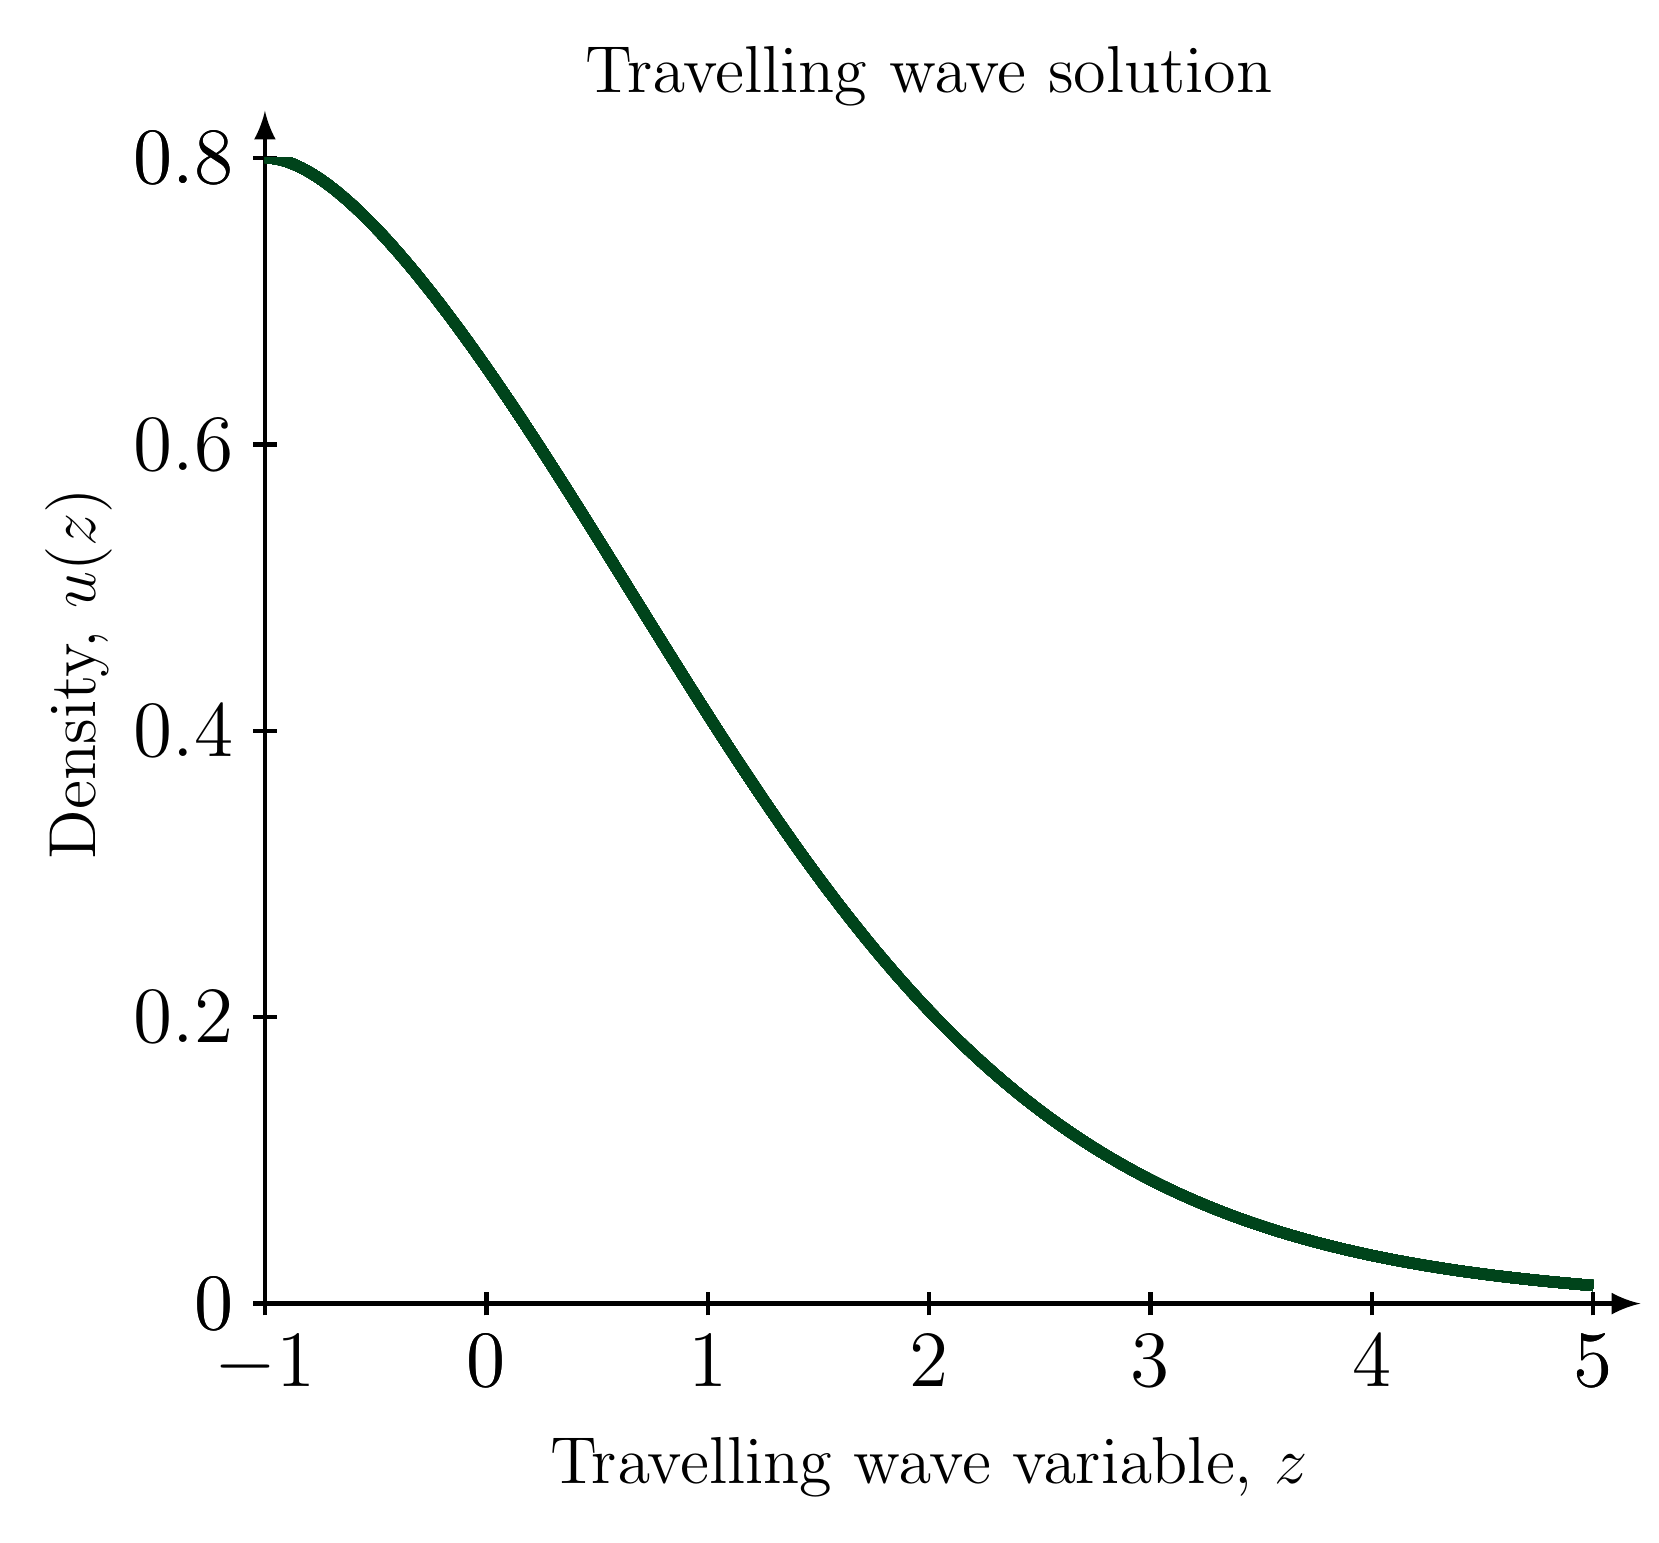
\begin{tikzpicture}[scale=2]
  % The axis of the plot
\begin{axis}[
    xlabel={Travelling wave variable, $z$},
    ylabel={Density, $u(z)$},
    title={Travelling wave solution},
    x label style={at={(axis description cs:0.5,-0.1)},anchor=north},
    y label style={at={(axis description cs:-0.1,0.55)},rotate=0,anchor=south},
    %scaled x ticks = false,
    xtick={-1,0,1,...,10},
    ytick={0,0.2,...,1.0},
    ymax = 0.8,
    ymin=0,
    xmin=-1,    
    extra y ticks={0,0.8},
    extra x ticks={0,5},% extra x tick labels={},    
    %xmax = 6,
    legend style={at={(axis description cs:0.45,0.6)},anchor=west,nodes={scale=1.75, transform shape}},
    label style={font=\large},
    title style={font=\large},    
    tick label style={font=\Large},
    legend cell align={left},
    grid style=dashed,
]
\addplot[
forget plot,
color=exp_1,line width=2pt,
]
coordinates {%
(-1.0,0.8)
(-0.979933110367893,0.7998802996323197)
(-0.959866220735786,0.7995316455518172)
(-0.939799331103679,0.7989686664342315)
(-0.919732441471572,0.7982047695699862)
(-0.8996655518394648,0.7972522555856665)
(-0.8795986622073578,0.7961224117058516)
(-0.8595317725752508,0.7948256148737269)
(-0.8394648829431438,0.7933714078766398)
(-0.8193979933110368,0.7917685725399882)
(-0.7993311036789298,0.7900252000434295)
(-0.7792642140468227,0.7881487509426632)
(-0.7591973244147157,0.7861461093204559)
(-0.7391304347826086,0.784023633798888)
(-0.7190635451505016,0.7817872022484336)
(-0.6989966555183946,0.7794422497075875)
(-0.6789297658862876,0.7769938114497514)
(-0.6588628762541806,0.774446553419733)
(-0.6387959866220736,0.7718048045425863)
(-0.6187290969899666,0.7690725847677562)
(-0.5986622073578596,0.7662536311000908)
(-0.5785953177257526,0.7633514218246813)
(-0.5585284280936454,0.7603691981486312)
(-0.5384615384615384,0.7573099843881764)
(-0.5183946488294314,0.7541766062657382)
(-0.4983277591973244,0.750971707053039)
(-0.4782608695652174,0.7476977653188627)
(-0.4581939799331104,0.7443571067815358)
(-0.4381270903010033,0.7409519193858108)
(-0.41806020066889626,0.7374842641023835)
(-0.39799331103678925,0.7339560868243299)
(-0.37792642140468224,0.7303692285400855)
(-0.35785953177257523,0.7267254344155136)
(-0.3377926421404682,0.7230263634373242)
(-0.3177257525083612,0.7192735953948975)
(-0.2976588628762542,0.715468639361365)
(-0.2775919732441472,0.7116129396390214)
(-0.2575250836120401,0.7077078828362365)
(-0.23745819397993306,0.7037548032198733)
(-0.21739130434782605,0.6997549883613848)
(-0.19732441471571904,0.6957096840505672)
(-0.17725752508361203,0.691620098369139)
(-0.15719063545150502,0.6874874065746939)
(-0.137123745819398,0.6833127549628811)
(-0.11705685618729089,0.6790972645113962)
(-0.09698996655518388,0.6748420330337627)
(-0.07692307692307687,0.6705481391881851)
(-0.05685618729096986,0.6662166453170358)
(-0.03678929765886285,0.6618485990135612)
(-0.01672240802675584,0.657445036223614)
(0.0033444816053511683,0.6530069831833845)
(0.02341137123745818,0.648535458024638)
(0.04347826086956519,0.644031472837882)
(0.0635451505016722,0.6394960350286075)
(0.08361204013377921,0.6349301485143479)
(0.10367892976588622,0.6303348151645952)
(0.12374581939799345,0.6257110358516449)
(0.14381270903010046,0.6210598114380332)
(0.16387959866220747,0.6163821436164816)
(0.18394648829431448,0.611679035535881)
(0.2040133779264215,0.6069514924733537)
(0.2240802675585285,0.6022005223836343)
(0.2441471571906355,0.5974271362078387)
(0.2642140468227425,0.5926323483105178)
(0.28428093645484953,0.5878171767595616)
(0.30434782608695654,0.5829826433825998)
(0.32441471571906355,0.5781297737956653)
(0.34448160535117056,0.5732595975857216)
(0.36454849498327757,0.5683731481928855)
(0.3846153846153846,0.5634714628535373)
(0.4046822742474916,0.5585555823302237)
(0.4247491638795986,0.5536265506419309)
(0.4448160535117056,0.5486854150405451)
(0.46488294314381284,0.5437332256882745)
(0.48494983277591985,0.5387710349964595)
(0.5050167224080269,0.5337998973550708)
(0.5250836120401339,0.5288208690248067)
(0.5451505016722409,0.5238350072583225)
(0.5652173913043479,0.5188433698261934)
(0.5852842809364549,0.5138470147640685)
(0.6053511705685619,0.5088469997297922)
(0.6254180602006689,0.5038443812236864)
(0.6454849498327759,0.49884021411699514)
(0.6655518394648829,0.4938355512920729)
(0.68561872909699,0.4888314426640525)
(0.705685618729097,0.4838289345958738)
(0.725752508361204,0.4788290695215183)
(0.745819397993311,0.47383288508354116)
(0.7658862876254182,0.4688414133313686)
(0.7859531772575252,0.4638556800695874)
(0.8060200668896322,0.45887670465963115)
(0.8260869565217392,0.45390549909091604)
(0.8461538461538463,0.4489430670509684)
(0.8662207357859533,0.4439904033601199)
(0.8862876254180603,0.43904849363848836)
(0.9063545150501673,0.4341183135202479)
(0.9264214046822743,0.42920082775968865)
(0.9464882943143813,0.4242969896760367)
(0.9665551839464883,0.41940774081263316)
(0.9866220735785953,0.41453401027066467)
(1.0066889632107023,0.4096767138361829)
(1.0267558528428093,0.404836753492283)
(1.0468227424749164,0.4000150170702445)
(1.0668896321070234,0.3952123777172501)
(1.0869565217391304,0.39042969309606956)
(1.1070234113712374,0.38566780497116915)
(1.1270903010033444,0.3809275388663621)
(1.1471571906354514,0.37620970365758455)
(1.1672240802675584,0.37151509088783635)
(1.1872909698996654,0.36684447442840007)
(1.2073578595317724,0.36219861018268035)
(1.2274247491638794,0.35757823579584846)
(1.247491638795987,0.35298407009451593)
(1.267558528428094,0.34841681283635645)
(1.287625418060201,0.34387714448334117)
(1.307692307692308,0.3393657260018602)
(1.327759197324415,0.334883198427433)
(1.347826086956522,0.3304301827059441)
(1.367892976588629,0.3260072794904346)
(1.387959866220736,0.3216150691590346)
(1.408026755852843,0.3172541115657907)
(1.42809364548495,0.3129249458358587)
(1.448160535117057,0.3086280903326475)
(1.468227424749164,0.30436404259183536)
(1.488294314381271,0.30013327929395534)
(1.508361204013378,0.29593625623004693)
(1.528428093645485,0.2917734083118474)
(1.548494983277592,0.2876451496060683)
(1.568561872909699,0.2835518733586398)
(1.588628762541806,0.27949395202560057)
(1.608695652173913,0.27547173745987635)
(1.62876254180602,0.2714855610020448)
(1.648829431438127,0.2675357336248416)
(1.6688963210702341,0.26362254596626933)
(1.6889632107023411,0.25974626856167077)
(1.7090301003344481,0.255907152128753)
(1.7290969899665551,0.2521054277432167)
(1.7491638795986622,0.24834130705410865)
(1.7692307692307692,0.24461498226405312)
(1.7892976588628762,0.24092662667502263)
(1.8093645484949832,0.2372763949479513)
(1.8294314381270902,0.2336644233669299)
(1.8494983277591972,0.23009083005330322)
(1.8695652173913042,0.22655571507987785)
(1.8896321070234112,0.22305916114692717)
(1.9096989966555187,0.2196012338104152)
(1.9297658862876257,0.21618198183486717)
(1.9498327759197327,0.21280143731019852)
(1.9698996655518397,0.20945961606691088)
(1.9899665551839467,0.20615651826575437)
(2.0100334448160537,0.20289212867369355)
(2.0301003344481607,0.19966641703603902)
(2.0501672240802677,0.19647933814011237)
(2.0702341137123748,0.19333083252007738)
(2.0903010033444818,0.19022082685991826)
(2.1103678929765888,0.18714923434879321)
(2.130434782608696,0.18411595500361078)
(2.150501672240803,0.18112087582787667)
(2.17056856187291,0.17816387159203895)
(2.190635451505017,0.175244805128103)
(2.210702341137124,0.17236352773232486)
(2.230769230769231,0.16951987938081337)
(2.250836120401338,0.1667136891232099)
(2.270903010033445,0.163944775712805)
(2.290969899665552,0.1612129479024892)
(2.311036789297659,0.15851800483673334)
(2.331103678929766,0.1558597362046108)
(2.351170568561873,0.1532379228339079)
(2.37123745819398,0.15065233710393242)
(2.391304347826087,0.14810274328444084)
(2.411371237458194,0.1455888978690934)
(2.431438127090301,0.1431105497692542)
(2.451505016722408,0.1406674409266675)
(2.471571906354515,0.13825930660818958)
(2.491638795986622,0.13588587575353983)
(2.511705685618729,0.1335468712017127)
(2.5317725752508364,0.131242010016428)
(2.5518394648829434,0.1289710040233326)
(2.5719063545150505,0.12673356005136244)
(2.5919732441471575,0.12452938026594515)
(2.6120401337792645,0.12235816249063045)
(2.6321070234113715,0.12021960017104799)
(2.6521739130434785,0.11811338293399008)
(2.6722408026755855,0.11603919701480943)
(2.6923076923076925,0.11399672543234791)
(2.7123745819397995,0.11198564827368945)
(2.7324414715719065,0.11000564295258643)
(2.7525083612040135,0.10805638429561414)
(2.7725752508361206,0.10613754501404882)
(2.7926421404682276,0.10424879593062077)
(2.8127090301003346,0.1023898061952523)
(2.8327759197324416,0.10056024352370016)
(2.8528428093645486,0.0987597743997618)
(2.8729096989966556,0.09698806421501638)
(2.8929765886287626,0.09524477761978399)
(2.9130434782608696,0.09352957868551089)
(2.9331103678929766,0.09184213109828095)
(2.9531772575250836,0.09018209835148198)
(2.9732441471571907,0.08854914390971554)
(2.9933110367892977,0.086942931375307)
(3.0133779264214047,0.08536312470005679)
(3.033444816053512,0.08380938832874436)
(3.0535117056856187,0.08228138735433792)
(3.073578595317726,0.08077878766710413)
(3.0936454849498327,0.07930125616057629)
(3.11371237458194,0.07784846083249865)
(3.1337792642140467,0.07642007088159002)
(3.153846153846154,0.07501575685691321)
(3.1739130434782608,0.07363519077595505)
(3.193979933110368,0.07227804645774501)
(3.2140468227424748,0.0709439987068491)
(3.2341137123745822,0.06963272516735151)
(3.254180602006689,0.06834390483996426)
(3.2742474916387962,0.06707721875939987)
(3.294314381270903,0.06583235006024382)
(3.3143812709030103,0.06460898407235618)
(3.334448160535117,0.06340680849539226)
(3.3545150501672243,0.062225513303871015)
(3.374581939799331,0.06106479086345808)
(3.3946488294314383,0.059924336010480674)
(3.414715719063545,0.05880384612077215)
(3.4347826086956523,0.05770302117067357)
(3.454849498327759,0.05662156381707954)
(3.4749163879598663,0.055559179465775876)
(3.494983277591974,0.054515576339632436)
(3.5150501672240804,0.05349046553010246)
(3.535117056856188,0.05248356061334376)
(3.5551839464882944,0.05149457809880519)
(3.575250836120402,0.05052323757616187)
(3.5953177257525084,0.04956926164992244)
(3.615384615384616,0.04863237599196789)
(3.6354515050167224,0.047712308932890114)
(3.65551839464883,0.04680879169575645)
(3.6755852842809364,0.04592155878961422)
(3.695652173913044,0.04505034783073824)
(3.7157190635451505,0.0441948995788828)
(3.735785953177258,0.04335495770053456)
(3.7558528428093645,0.04253026867069133)
(3.775919732441472,0.041720582320322865)
(3.7959866220735785,0.04092565161955228)
(3.816053511705686,0.040145232695715925)
(3.8361204013377925,0.03937908471280989)
(3.8561872909699,0.03862696960970699)
(3.8762541806020065,0.03788865263717003)
(3.896321070234114,0.037163902177448825)
(3.9163879598662206,0.03645248973601051)
(3.936454849498328,0.03575418989640538)
(3.9565217391304346,0.035068780053049364)
(3.976588628762542,0.03439604074341259)
(3.9966555183946486,0.03373575557041009)
(4.016722408026756,0.033087711168429845)
(4.036789297658863,0.03245169713563765)
(4.05685618729097,0.03182750605482606)
(4.076923076923077,0.031214933515656178)
(4.096989966555184,0.030613778083990587)
(4.117056856187291,0.030023841240709708)
(4.137123745819398,0.02944492726864721)
(4.157190635451506,0.02887684340877022)
(4.177257525083612,0.028319399784123494)
(4.19732441471572,0.027772409372935944)
(4.217391304347826,0.027235687912175878)
(4.237458193979934,0.026709053948558367)
(4.25752508361204,0.026192328822269528)
(4.277591973244148,0.025685336631400293)
(4.297658862876254,0.025187904174334502)
(4.317725752508362,0.024699860913535022)
(4.337792642140468,0.024221039009902568)
(4.357859531772576,0.023751273273148524)
(4.377926421404682,0.023290401128805257)
(4.39799331103679,0.022838262545582938)
(4.418060200668896,0.02239470006848357)
(4.438127090301004,0.021959558780367552)
(4.45819397993311,0.021532686270159862)
(4.478260869565218,0.021113932564241374)
(4.498327759197324,0.020703150133824275)
(4.518394648829432,0.020300193888211082)
(4.538461538461538,0.019904921129637983)
(4.558528428093646,0.019517191526265753)
(4.578595317725752,0.019136867085171)
(4.59866220735786,0.018763812124895182)
(4.618729096989966,0.01839789314646722)
(4.638795986622074,0.01803897886846312)
(4.65886287625418,0.01768694027482413)
(4.678929765886288,0.017341650531776366)
(4.698996655518394,0.017002984959118804)
(4.719063545150502,0.01667082100151099)
(4.739130434782608,0.016345038199758632)
(4.759197324414716,0.016025518139530952)
(4.7792642140468224,0.015712144430794227)
(4.79933110367893,0.01540480270389043)
(4.819397993311037,0.015103380565133153)
(4.839464882943144,0.014807767567672795)
(4.859531772575251,0.014517855182361795)
(4.879598662207358,0.01423353676861998)
(4.899665551839465,0.013954707578129404)
(4.919732441471572,0.013681264724478042)
(4.939799331103679,0.013413107102207947)
(4.959866220735786,0.01315013538669457)
(4.979933110367893,0.012892252005810028)
(5.0,0.0126393611114975)
};
\addplot[
forget plot,
color=exp_1,line width=2pt,
]
coordinates {%
(-1.0,0.8)
(-0.979933110367893,0.7998802996323197)
(-0.959866220735786,0.7995316455518172)
(-0.939799331103679,0.7989686664342315)
(-0.919732441471572,0.7982047695699862)
(-0.8996655518394648,0.7972522555856665)
(-0.8795986622073578,0.7961224117058516)
(-0.8595317725752508,0.7948256148737269)
(-0.8394648829431438,0.7933714078766398)
(-0.8193979933110368,0.7917685725399882)
(-0.7993311036789298,0.7900252000434295)
(-0.7792642140468227,0.7881487509426632)
(-0.7591973244147157,0.7861461093204559)
(-0.7391304347826086,0.784023633798888)
(-0.7190635451505016,0.7817872022484336)
(-0.6989966555183946,0.7794422497075875)
(-0.6789297658862876,0.7769938114497514)
(-0.6588628762541806,0.774446553419733)
(-0.6387959866220736,0.7718048045425863)
(-0.6187290969899666,0.7690725847677562)
(-0.5986622073578596,0.7662536311000908)
(-0.5785953177257526,0.7633514218246813)
(-0.5585284280936454,0.7603691981486312)
(-0.5384615384615384,0.7573099843881764)
(-0.5183946488294314,0.7541766062657382)
(-0.4983277591973244,0.750971707053039)
(-0.4782608695652174,0.7476977653188627)
(-0.4581939799331104,0.7443571067815358)
(-0.4381270903010033,0.7409519193858108)
(-0.41806020066889626,0.7374842641023835)
(-0.39799331103678925,0.7339560868243299)
(-0.37792642140468224,0.7303692285400855)
(-0.35785953177257523,0.7267254344155136)
(-0.3377926421404682,0.7230263634373242)
(-0.3177257525083612,0.7192735953948975)
(-0.2976588628762542,0.715468639361365)
(-0.2775919732441472,0.7116129396390214)
(-0.2575250836120401,0.7077078828362365)
(-0.23745819397993306,0.7037548032198733)
(-0.21739130434782605,0.6997549883613848)
(-0.19732441471571904,0.6957096840505672)
(-0.17725752508361203,0.691620098369139)
(-0.15719063545150502,0.6874874065746939)
(-0.137123745819398,0.6833127549628811)
(-0.11705685618729089,0.6790972645113962)
(-0.09698996655518388,0.6748420330337627)
(-0.07692307692307687,0.6705481391881851)
(-0.05685618729096986,0.6662166453170358)
(-0.03678929765886285,0.6618485990135612)
(-0.01672240802675584,0.657445036223614)
(0.0033444816053511683,0.6530069831833845)
(0.02341137123745818,0.648535458024638)
(0.04347826086956519,0.644031472837882)
(0.0635451505016722,0.6394960350286075)
(0.08361204013377921,0.6349301485143479)
(0.10367892976588622,0.6303348151645952)
(0.12374581939799345,0.6257110358516449)
(0.14381270903010046,0.6210598114380332)
(0.16387959866220747,0.6163821436164816)
(0.18394648829431448,0.611679035535881)
(0.2040133779264215,0.6069514924733537)
(0.2240802675585285,0.6022005223836343)
(0.2441471571906355,0.5974271362078387)
(0.2642140468227425,0.5926323483105178)
(0.28428093645484953,0.5878171767595616)
(0.30434782608695654,0.5829826433825998)
(0.32441471571906355,0.5781297737956653)
(0.34448160535117056,0.5732595975857216)
(0.36454849498327757,0.5683731481928855)
(0.3846153846153846,0.5634714628535373)
(0.4046822742474916,0.5585555823302237)
(0.4247491638795986,0.5536265506419309)
(0.4448160535117056,0.5486854150405451)
(0.46488294314381284,0.5437332256882745)
(0.48494983277591985,0.5387710349964595)
(0.5050167224080269,0.5337998973550708)
(0.5250836120401339,0.5288208690248067)
(0.5451505016722409,0.5238350072583225)
(0.5652173913043479,0.5188433698261934)
(0.5852842809364549,0.5138470147640685)
(0.6053511705685619,0.5088469997297922)
(0.6254180602006689,0.5038443812236864)
(0.6454849498327759,0.49884021411699514)
(0.6655518394648829,0.4938355512920729)
(0.68561872909699,0.4888314426640525)
(0.705685618729097,0.4838289345958738)
(0.725752508361204,0.4788290695215183)
(0.745819397993311,0.47383288508354116)
(0.7658862876254182,0.4688414133313686)
(0.7859531772575252,0.4638556800695874)
(0.8060200668896322,0.45887670465963115)
(0.8260869565217392,0.45390549909091604)
(0.8461538461538463,0.4489430670509684)
(0.8662207357859533,0.4439904033601199)
(0.8862876254180603,0.43904849363848836)
(0.9063545150501673,0.4341183135202479)
(0.9264214046822743,0.42920082775968865)
(0.9464882943143813,0.4242969896760367)
(0.9665551839464883,0.41940774081263316)
(0.9866220735785953,0.41453401027066467)
(1.0066889632107023,0.4096767138361829)
(1.0267558528428093,0.404836753492283)
(1.0468227424749164,0.4000150170702445)
(1.0668896321070234,0.3952123777172501)
(1.0869565217391304,0.39042969309606956)
(1.1070234113712374,0.38566780497116915)
(1.1270903010033444,0.3809275388663621)
(1.1471571906354514,0.37620970365758455)
(1.1672240802675584,0.37151509088783635)
(1.1872909698996654,0.36684447442840007)
(1.2073578595317724,0.36219861018268035)
(1.2274247491638794,0.35757823579584846)
(1.247491638795987,0.35298407009451593)
(1.267558528428094,0.34841681283635645)
(1.287625418060201,0.34387714448334117)
(1.307692307692308,0.3393657260018602)
(1.327759197324415,0.334883198427433)
(1.347826086956522,0.3304301827059441)
(1.367892976588629,0.3260072794904346)
(1.387959866220736,0.3216150691590346)
(1.408026755852843,0.3172541115657907)
(1.42809364548495,0.3129249458358587)
(1.448160535117057,0.3086280903326475)
(1.468227424749164,0.30436404259183536)
(1.488294314381271,0.30013327929395534)
(1.508361204013378,0.29593625623004693)
(1.528428093645485,0.2917734083118474)
(1.548494983277592,0.2876451496060683)
(1.568561872909699,0.2835518733586398)
(1.588628762541806,0.27949395202560057)
(1.608695652173913,0.27547173745987635)
(1.62876254180602,0.2714855610020448)
(1.648829431438127,0.2675357336248416)
(1.6688963210702341,0.26362254596626933)
(1.6889632107023411,0.25974626856167077)
(1.7090301003344481,0.255907152128753)
(1.7290969899665551,0.2521054277432167)
(1.7491638795986622,0.24834130705410865)
(1.7692307692307692,0.24461498226405312)
(1.7892976588628762,0.24092662667502263)
(1.8093645484949832,0.2372763949479513)
(1.8294314381270902,0.2336644233669299)
(1.8494983277591972,0.23009083005330322)
(1.8695652173913042,0.22655571507987785)
(1.8896321070234112,0.22305916114692717)
(1.9096989966555187,0.2196012338104152)
(1.9297658862876257,0.21618198183486717)
(1.9498327759197327,0.21280143731019852)
(1.9698996655518397,0.20945961606691088)
(1.9899665551839467,0.20615651826575437)
(2.0100334448160537,0.20289212867369355)
(2.0301003344481607,0.19966641703603902)
(2.0501672240802677,0.19647933814011237)
(2.0702341137123748,0.19333083252007738)
(2.0903010033444818,0.19022082685991826)
(2.1103678929765888,0.18714923434879321)
(2.130434782608696,0.18411595500361078)
(2.150501672240803,0.18112087582787667)
(2.17056856187291,0.17816387159203895)
(2.190635451505017,0.175244805128103)
(2.210702341137124,0.17236352773232486)
(2.230769230769231,0.16951987938081337)
(2.250836120401338,0.1667136891232099)
(2.270903010033445,0.163944775712805)
(2.290969899665552,0.1612129479024892)
(2.311036789297659,0.15851800483673334)
(2.331103678929766,0.1558597362046108)
(2.351170568561873,0.1532379228339079)
(2.37123745819398,0.15065233710393242)
(2.391304347826087,0.14810274328444084)
(2.411371237458194,0.1455888978690934)
(2.431438127090301,0.1431105497692542)
(2.451505016722408,0.1406674409266675)
(2.471571906354515,0.13825930660818958)
(2.491638795986622,0.13588587575353983)
(2.511705685618729,0.1335468712017127)
(2.5317725752508364,0.131242010016428)
(2.5518394648829434,0.1289710040233326)
(2.5719063545150505,0.12673356005136244)
(2.5919732441471575,0.12452938026594515)
(2.6120401337792645,0.12235816249063045)
(2.6321070234113715,0.12021960017104799)
(2.6521739130434785,0.11811338293399008)
(2.6722408026755855,0.11603919701480943)
(2.6923076923076925,0.11399672543234791)
(2.7123745819397995,0.11198564827368945)
(2.7324414715719065,0.11000564295258643)
(2.7525083612040135,0.10805638429561414)
(2.7725752508361206,0.10613754501404882)
(2.7926421404682276,0.10424879593062077)
(2.8127090301003346,0.1023898061952523)
(2.8327759197324416,0.10056024352370016)
(2.8528428093645486,0.0987597743997618)
(2.8729096989966556,0.09698806421501638)
(2.8929765886287626,0.09524477761978399)
(2.9130434782608696,0.09352957868551089)
(2.9331103678929766,0.09184213109828095)
(2.9531772575250836,0.09018209835148198)
(2.9732441471571907,0.08854914390971554)
(2.9933110367892977,0.086942931375307)
(3.0133779264214047,0.08536312470005679)
(3.033444816053512,0.08380938832874436)
(3.0535117056856187,0.08228138735433792)
(3.073578595317726,0.08077878766710413)
(3.0936454849498327,0.07930125616057629)
(3.11371237458194,0.07784846083249865)
(3.1337792642140467,0.07642007088159002)
(3.153846153846154,0.07501575685691321)
(3.1739130434782608,0.07363519077595505)
(3.193979933110368,0.07227804645774501)
(3.2140468227424748,0.0709439987068491)
(3.2341137123745822,0.06963272516735151)
(3.254180602006689,0.06834390483996426)
(3.2742474916387962,0.06707721875939987)
(3.294314381270903,0.06583235006024382)
(3.3143812709030103,0.06460898407235618)
(3.334448160535117,0.06340680849539226)
(3.3545150501672243,0.062225513303871015)
(3.374581939799331,0.06106479086345808)
(3.3946488294314383,0.059924336010480674)
(3.414715719063545,0.05880384612077215)
(3.4347826086956523,0.05770302117067357)
(3.454849498327759,0.05662156381707954)
(3.4749163879598663,0.055559179465775876)
(3.494983277591974,0.054515576339632436)
(3.5150501672240804,0.05349046553010246)
(3.535117056856188,0.05248356061334376)
(3.5551839464882944,0.05149457809880519)
(3.575250836120402,0.05052323757616187)
(3.5953177257525084,0.04956926164992244)
(3.615384615384616,0.04863237599196789)
(3.6354515050167224,0.047712308932890114)
(3.65551839464883,0.04680879169575645)
(3.6755852842809364,0.04592155878961422)
(3.695652173913044,0.04505034783073824)
(3.7157190635451505,0.0441948995788828)
(3.735785953177258,0.04335495770053456)
(3.7558528428093645,0.04253026867069133)
(3.775919732441472,0.041720582320322865)
(3.7959866220735785,0.04092565161955228)
(3.816053511705686,0.040145232695715925)
(3.8361204013377925,0.03937908471280989)
(3.8561872909699,0.03862696960970699)
(3.8762541806020065,0.03788865263717003)
(3.896321070234114,0.037163902177448825)
(3.9163879598662206,0.03645248973601051)
(3.936454849498328,0.03575418989640538)
(3.9565217391304346,0.035068780053049364)
(3.976588628762542,0.03439604074341259)
(3.9966555183946486,0.03373575557041009)
(4.016722408026756,0.033087711168429845)
(4.036789297658863,0.03245169713563765)
(4.05685618729097,0.03182750605482606)
(4.076923076923077,0.031214933515656178)
(4.096989966555184,0.030613778083990587)
(4.117056856187291,0.030023841240709708)
(4.137123745819398,0.02944492726864721)
(4.157190635451506,0.02887684340877022)
(4.177257525083612,0.028319399784123494)
(4.19732441471572,0.027772409372935944)
(4.217391304347826,0.027235687912175878)
(4.237458193979934,0.026709053948558367)
(4.25752508361204,0.026192328822269528)
(4.277591973244148,0.025685336631400293)
(4.297658862876254,0.025187904174334502)
(4.317725752508362,0.024699860913535022)
(4.337792642140468,0.024221039009902568)
(4.357859531772576,0.023751273273148524)
(4.377926421404682,0.023290401128805257)
(4.39799331103679,0.022838262545582938)
(4.418060200668896,0.02239470006848357)
(4.438127090301004,0.021959558780367552)
(4.45819397993311,0.021532686270159862)
(4.478260869565218,0.021113932564241374)
(4.498327759197324,0.020703150133824275)
(4.518394648829432,0.020300193888211082)
(4.538461538461538,0.019904921129637983)
(4.558528428093646,0.019517191526265753)
(4.578595317725752,0.019136867085171)
(4.59866220735786,0.018763812124895182)
(4.618729096989966,0.01839789314646722)
(4.638795986622074,0.01803897886846312)
(4.65886287625418,0.01768694027482413)
(4.678929765886288,0.017341650531776366)
(4.698996655518394,0.017002984959118804)
(4.719063545150502,0.01667082100151099)
(4.739130434782608,0.016345038199758632)
(4.759197324414716,0.016025518139530952)
(4.7792642140468224,0.015712144430794227)
(4.79933110367893,0.01540480270389043)
(4.819397993311037,0.015103380565133153)
(4.839464882943144,0.014807767567672795)
(4.859531772575251,0.014517855182361795)
(4.879598662207358,0.01423353676861998)
(4.899665551839465,0.013954707578129404)
(4.919732441471572,0.013681264724478042)
(4.939799331103679,0.013413107102207947)
(4.959866220735786,0.01315013538669457)
(4.979933110367893,0.012892252005810028)
(5.0,0.0126393611114975)
};
\addplot[
forget plot,
color=exp_1,line width=2pt,
]
coordinates {%
(-1.0,0.8)
(-0.979933110367893,0.7998802996323197)
(-0.959866220735786,0.7995316455518172)
(-0.939799331103679,0.7989686664342315)
(-0.919732441471572,0.7982047695699862)
(-0.8996655518394648,0.7972522555856665)
(-0.8795986622073578,0.7961224117058516)
(-0.8595317725752508,0.7948256148737269)
(-0.8394648829431438,0.7933714078766398)
(-0.8193979933110368,0.7917685725399882)
(-0.7993311036789298,0.7900252000434295)
(-0.7792642140468227,0.7881487509426632)
(-0.7591973244147157,0.7861461093204559)
(-0.7391304347826086,0.784023633798888)
(-0.7190635451505016,0.7817872022484336)
(-0.6989966555183946,0.7794422497075875)
(-0.6789297658862876,0.7769938114497514)
(-0.6588628762541806,0.774446553419733)
(-0.6387959866220736,0.7718048045425863)
(-0.6187290969899666,0.7690725847677562)
(-0.5986622073578596,0.7662536311000908)
(-0.5785953177257526,0.7633514218246813)
(-0.5585284280936454,0.7603691981486312)
(-0.5384615384615384,0.7573099843881764)
(-0.5183946488294314,0.7541766062657382)
(-0.4983277591973244,0.750971707053039)
(-0.4782608695652174,0.7476977653188627)
(-0.4581939799331104,0.7443571067815358)
(-0.4381270903010033,0.7409519193858108)
(-0.41806020066889626,0.7374842641023835)
(-0.39799331103678925,0.7339560868243299)
(-0.37792642140468224,0.7303692285400855)
(-0.35785953177257523,0.7267254344155136)
(-0.3377926421404682,0.7230263634373242)
(-0.3177257525083612,0.7192735953948975)
(-0.2976588628762542,0.715468639361365)
(-0.2775919732441472,0.7116129396390214)
(-0.2575250836120401,0.7077078828362365)
(-0.23745819397993306,0.7037548032198733)
(-0.21739130434782605,0.6997549883613848)
(-0.19732441471571904,0.6957096840505672)
(-0.17725752508361203,0.691620098369139)
(-0.15719063545150502,0.6874874065746939)
(-0.137123745819398,0.6833127549628811)
(-0.11705685618729089,0.6790972645113962)
(-0.09698996655518388,0.6748420330337627)
(-0.07692307692307687,0.6705481391881851)
(-0.05685618729096986,0.6662166453170358)
(-0.03678929765886285,0.6618485990135612)
(-0.01672240802675584,0.657445036223614)
(0.0033444816053511683,0.6530069831833845)
(0.02341137123745818,0.648535458024638)
(0.04347826086956519,0.644031472837882)
(0.0635451505016722,0.6394960350286075)
(0.08361204013377921,0.6349301485143479)
(0.10367892976588622,0.6303348151645952)
(0.12374581939799345,0.6257110358516449)
(0.14381270903010046,0.6210598114380332)
(0.16387959866220747,0.6163821436164816)
(0.18394648829431448,0.611679035535881)
(0.2040133779264215,0.6069514924733537)
(0.2240802675585285,0.6022005223836343)
(0.2441471571906355,0.5974271362078387)
(0.2642140468227425,0.5926323483105178)
(0.28428093645484953,0.5878171767595616)
(0.30434782608695654,0.5829826433825998)
(0.32441471571906355,0.5781297737956653)
(0.34448160535117056,0.5732595975857216)
(0.36454849498327757,0.5683731481928855)
(0.3846153846153846,0.5634714628535373)
(0.4046822742474916,0.5585555823302237)
(0.4247491638795986,0.5536265506419309)
(0.4448160535117056,0.5486854150405451)
(0.46488294314381284,0.5437332256882745)
(0.48494983277591985,0.5387710349964595)
(0.5050167224080269,0.5337998973550708)
(0.5250836120401339,0.5288208690248067)
(0.5451505016722409,0.5238350072583225)
(0.5652173913043479,0.5188433698261934)
(0.5852842809364549,0.5138470147640685)
(0.6053511705685619,0.5088469997297922)
(0.6254180602006689,0.5038443812236864)
(0.6454849498327759,0.49884021411699514)
(0.6655518394648829,0.4938355512920729)
(0.68561872909699,0.4888314426640525)
(0.705685618729097,0.4838289345958738)
(0.725752508361204,0.4788290695215183)
(0.745819397993311,0.47383288508354116)
(0.7658862876254182,0.4688414133313686)
(0.7859531772575252,0.4638556800695874)
(0.8060200668896322,0.45887670465963115)
(0.8260869565217392,0.45390549909091604)
(0.8461538461538463,0.4489430670509684)
(0.8662207357859533,0.4439904033601199)
(0.8862876254180603,0.43904849363848836)
(0.9063545150501673,0.4341183135202479)
(0.9264214046822743,0.42920082775968865)
(0.9464882943143813,0.4242969896760367)
(0.9665551839464883,0.41940774081263316)
(0.9866220735785953,0.41453401027066467)
(1.0066889632107023,0.4096767138361829)
(1.0267558528428093,0.404836753492283)
(1.0468227424749164,0.4000150170702445)
(1.0668896321070234,0.3952123777172501)
(1.0869565217391304,0.39042969309606956)
(1.1070234113712374,0.38566780497116915)
(1.1270903010033444,0.3809275388663621)
(1.1471571906354514,0.37620970365758455)
(1.1672240802675584,0.37151509088783635)
(1.1872909698996654,0.36684447442840007)
(1.2073578595317724,0.36219861018268035)
(1.2274247491638794,0.35757823579584846)
(1.247491638795987,0.35298407009451593)
(1.267558528428094,0.34841681283635645)
(1.287625418060201,0.34387714448334117)
(1.307692307692308,0.3393657260018602)
(1.327759197324415,0.334883198427433)
(1.347826086956522,0.3304301827059441)
(1.367892976588629,0.3260072794904346)
(1.387959866220736,0.3216150691590346)
(1.408026755852843,0.3172541115657907)
(1.42809364548495,0.3129249458358587)
(1.448160535117057,0.3086280903326475)
(1.468227424749164,0.30436404259183536)
(1.488294314381271,0.30013327929395534)
(1.508361204013378,0.29593625623004693)
(1.528428093645485,0.2917734083118474)
(1.548494983277592,0.2876451496060683)
(1.568561872909699,0.2835518733586398)
(1.588628762541806,0.27949395202560057)
(1.608695652173913,0.27547173745987635)
(1.62876254180602,0.2714855610020448)
(1.648829431438127,0.2675357336248416)
(1.6688963210702341,0.26362254596626933)
(1.6889632107023411,0.25974626856167077)
(1.7090301003344481,0.255907152128753)
(1.7290969899665551,0.2521054277432167)
(1.7491638795986622,0.24834130705410865)
(1.7692307692307692,0.24461498226405312)
(1.7892976588628762,0.24092662667502263)
(1.8093645484949832,0.2372763949479513)
(1.8294314381270902,0.2336644233669299)
(1.8494983277591972,0.23009083005330322)
(1.8695652173913042,0.22655571507987785)
(1.8896321070234112,0.22305916114692717)
(1.9096989966555187,0.2196012338104152)
(1.9297658862876257,0.21618198183486717)
(1.9498327759197327,0.21280143731019852)
(1.9698996655518397,0.20945961606691088)
(1.9899665551839467,0.20615651826575437)
(2.0100334448160537,0.20289212867369355)
(2.0301003344481607,0.19966641703603902)
(2.0501672240802677,0.19647933814011237)
(2.0702341137123748,0.19333083252007738)
(2.0903010033444818,0.19022082685991826)
(2.1103678929765888,0.18714923434879321)
(2.130434782608696,0.18411595500361078)
(2.150501672240803,0.18112087582787667)
(2.17056856187291,0.17816387159203895)
(2.190635451505017,0.175244805128103)
(2.210702341137124,0.17236352773232486)
(2.230769230769231,0.16951987938081337)
(2.250836120401338,0.1667136891232099)
(2.270903010033445,0.163944775712805)
(2.290969899665552,0.1612129479024892)
(2.311036789297659,0.15851800483673334)
(2.331103678929766,0.1558597362046108)
(2.351170568561873,0.1532379228339079)
(2.37123745819398,0.15065233710393242)
(2.391304347826087,0.14810274328444084)
(2.411371237458194,0.1455888978690934)
(2.431438127090301,0.1431105497692542)
(2.451505016722408,0.1406674409266675)
(2.471571906354515,0.13825930660818958)
(2.491638795986622,0.13588587575353983)
(2.511705685618729,0.1335468712017127)
(2.5317725752508364,0.131242010016428)
(2.5518394648829434,0.1289710040233326)
(2.5719063545150505,0.12673356005136244)
(2.5919732441471575,0.12452938026594515)
(2.6120401337792645,0.12235816249063045)
(2.6321070234113715,0.12021960017104799)
(2.6521739130434785,0.11811338293399008)
(2.6722408026755855,0.11603919701480943)
(2.6923076923076925,0.11399672543234791)
(2.7123745819397995,0.11198564827368945)
(2.7324414715719065,0.11000564295258643)
(2.7525083612040135,0.10805638429561414)
(2.7725752508361206,0.10613754501404882)
(2.7926421404682276,0.10424879593062077)
(2.8127090301003346,0.1023898061952523)
(2.8327759197324416,0.10056024352370016)
(2.8528428093645486,0.0987597743997618)
(2.8729096989966556,0.09698806421501638)
(2.8929765886287626,0.09524477761978399)
(2.9130434782608696,0.09352957868551089)
(2.9331103678929766,0.09184213109828095)
(2.9531772575250836,0.09018209835148198)
(2.9732441471571907,0.08854914390971554)
(2.9933110367892977,0.086942931375307)
(3.0133779264214047,0.08536312470005679)
(3.033444816053512,0.08380938832874436)
(3.0535117056856187,0.08228138735433792)
(3.073578595317726,0.08077878766710413)
(3.0936454849498327,0.07930125616057629)
(3.11371237458194,0.07784846083249865)
(3.1337792642140467,0.07642007088159002)
(3.153846153846154,0.07501575685691321)
(3.1739130434782608,0.07363519077595505)
(3.193979933110368,0.07227804645774501)
(3.2140468227424748,0.0709439987068491)
(3.2341137123745822,0.06963272516735151)
(3.254180602006689,0.06834390483996426)
(3.2742474916387962,0.06707721875939987)
(3.294314381270903,0.06583235006024382)
(3.3143812709030103,0.06460898407235618)
(3.334448160535117,0.06340680849539226)
(3.3545150501672243,0.062225513303871015)
(3.374581939799331,0.06106479086345808)
(3.3946488294314383,0.059924336010480674)
(3.414715719063545,0.05880384612077215)
(3.4347826086956523,0.05770302117067357)
(3.454849498327759,0.05662156381707954)
(3.4749163879598663,0.055559179465775876)
(3.494983277591974,0.054515576339632436)
(3.5150501672240804,0.05349046553010246)
(3.535117056856188,0.05248356061334376)
(3.5551839464882944,0.05149457809880519)
(3.575250836120402,0.05052323757616187)
(3.5953177257525084,0.04956926164992244)
(3.615384615384616,0.04863237599196789)
(3.6354515050167224,0.047712308932890114)
(3.65551839464883,0.04680879169575645)
(3.6755852842809364,0.04592155878961422)
(3.695652173913044,0.04505034783073824)
(3.7157190635451505,0.0441948995788828)
(3.735785953177258,0.04335495770053456)
(3.7558528428093645,0.04253026867069133)
(3.775919732441472,0.041720582320322865)
(3.7959866220735785,0.04092565161955228)
(3.816053511705686,0.040145232695715925)
(3.8361204013377925,0.03937908471280989)
(3.8561872909699,0.03862696960970699)
(3.8762541806020065,0.03788865263717003)
(3.896321070234114,0.037163902177448825)
(3.9163879598662206,0.03645248973601051)
(3.936454849498328,0.03575418989640538)
(3.9565217391304346,0.035068780053049364)
(3.976588628762542,0.03439604074341259)
(3.9966555183946486,0.03373575557041009)
(4.016722408026756,0.033087711168429845)
(4.036789297658863,0.03245169713563765)
(4.05685618729097,0.03182750605482606)
(4.076923076923077,0.031214933515656178)
(4.096989966555184,0.030613778083990587)
(4.117056856187291,0.030023841240709708)
(4.137123745819398,0.02944492726864721)
(4.157190635451506,0.02887684340877022)
(4.177257525083612,0.028319399784123494)
(4.19732441471572,0.027772409372935944)
(4.217391304347826,0.027235687912175878)
(4.237458193979934,0.026709053948558367)
(4.25752508361204,0.026192328822269528)
(4.277591973244148,0.025685336631400293)
(4.297658862876254,0.025187904174334502)
(4.317725752508362,0.024699860913535022)
(4.337792642140468,0.024221039009902568)
(4.357859531772576,0.023751273273148524)
(4.377926421404682,0.023290401128805257)
(4.39799331103679,0.022838262545582938)
(4.418060200668896,0.02239470006848357)
(4.438127090301004,0.021959558780367552)
(4.45819397993311,0.021532686270159862)
(4.478260869565218,0.021113932564241374)
(4.498327759197324,0.020703150133824275)
(4.518394648829432,0.020300193888211082)
(4.538461538461538,0.019904921129637983)
(4.558528428093646,0.019517191526265753)
(4.578595317725752,0.019136867085171)
(4.59866220735786,0.018763812124895182)
(4.618729096989966,0.01839789314646722)
(4.638795986622074,0.01803897886846312)
(4.65886287625418,0.01768694027482413)
(4.678929765886288,0.017341650531776366)
(4.698996655518394,0.017002984959118804)
(4.719063545150502,0.01667082100151099)
(4.739130434782608,0.016345038199758632)
(4.759197324414716,0.016025518139530952)
(4.7792642140468224,0.015712144430794227)
(4.79933110367893,0.01540480270389043)
(4.819397993311037,0.015103380565133153)
(4.839464882943144,0.014807767567672795)
(4.859531772575251,0.014517855182361795)
(4.879598662207358,0.01423353676861998)
(4.899665551839465,0.013954707578129404)
(4.919732441471572,0.013681264724478042)
(4.939799331103679,0.013413107102207947)
(4.959866220735786,0.01315013538669457)
(4.979933110367893,0.012892252005810028)
(5.0,0.0126393611114975)
};
\addplot[
forget plot,
color=exp_1,line width=2pt,
]
coordinates {%
(-1.0,0.8)
(-0.979933110367893,0.7998802996323197)
(-0.959866220735786,0.7995316455518172)
(-0.939799331103679,0.7989686664342315)
(-0.919732441471572,0.7982047695699862)
(-0.8996655518394648,0.7972522555856665)
(-0.8795986622073578,0.7961224117058516)
(-0.8595317725752508,0.7948256148737269)
(-0.8394648829431438,0.7933714078766398)
(-0.8193979933110368,0.7917685725399882)
(-0.7993311036789298,0.7900252000434295)
(-0.7792642140468227,0.7881487509426632)
(-0.7591973244147157,0.7861461093204559)
(-0.7391304347826086,0.784023633798888)
(-0.7190635451505016,0.7817872022484336)
(-0.6989966555183946,0.7794422497075875)
(-0.6789297658862876,0.7769938114497514)
(-0.6588628762541806,0.774446553419733)
(-0.6387959866220736,0.7718048045425863)
(-0.6187290969899666,0.7690725847677562)
(-0.5986622073578596,0.7662536311000908)
(-0.5785953177257526,0.7633514218246813)
(-0.5585284280936454,0.7603691981486312)
(-0.5384615384615384,0.7573099843881764)
(-0.5183946488294314,0.7541766062657382)
(-0.4983277591973244,0.750971707053039)
(-0.4782608695652174,0.7476977653188627)
(-0.4581939799331104,0.7443571067815358)
(-0.4381270903010033,0.7409519193858108)
(-0.41806020066889626,0.7374842641023835)
(-0.39799331103678925,0.7339560868243299)
(-0.37792642140468224,0.7303692285400855)
(-0.35785953177257523,0.7267254344155136)
(-0.3377926421404682,0.7230263634373242)
(-0.3177257525083612,0.7192735953948975)
(-0.2976588628762542,0.715468639361365)
(-0.2775919732441472,0.7116129396390214)
(-0.2575250836120401,0.7077078828362365)
(-0.23745819397993306,0.7037548032198733)
(-0.21739130434782605,0.6997549883613848)
(-0.19732441471571904,0.6957096840505672)
(-0.17725752508361203,0.691620098369139)
(-0.15719063545150502,0.6874874065746939)
(-0.137123745819398,0.6833127549628811)
(-0.11705685618729089,0.6790972645113962)
(-0.09698996655518388,0.6748420330337627)
(-0.07692307692307687,0.6705481391881851)
(-0.05685618729096986,0.6662166453170358)
(-0.03678929765886285,0.6618485990135612)
(-0.01672240802675584,0.657445036223614)
(0.0033444816053511683,0.6530069831833845)
(0.02341137123745818,0.648535458024638)
(0.04347826086956519,0.644031472837882)
(0.0635451505016722,0.6394960350286075)
(0.08361204013377921,0.6349301485143479)
(0.10367892976588622,0.6303348151645952)
(0.12374581939799345,0.6257110358516449)
(0.14381270903010046,0.6210598114380332)
(0.16387959866220747,0.6163821436164816)
(0.18394648829431448,0.611679035535881)
(0.2040133779264215,0.6069514924733537)
(0.2240802675585285,0.6022005223836343)
(0.2441471571906355,0.5974271362078387)
(0.2642140468227425,0.5926323483105178)
(0.28428093645484953,0.5878171767595616)
(0.30434782608695654,0.5829826433825998)
(0.32441471571906355,0.5781297737956653)
(0.34448160535117056,0.5732595975857216)
(0.36454849498327757,0.5683731481928855)
(0.3846153846153846,0.5634714628535373)
(0.4046822742474916,0.5585555823302237)
(0.4247491638795986,0.5536265506419309)
(0.4448160535117056,0.5486854150405451)
(0.46488294314381284,0.5437332256882745)
(0.48494983277591985,0.5387710349964595)
(0.5050167224080269,0.5337998973550708)
(0.5250836120401339,0.5288208690248067)
(0.5451505016722409,0.5238350072583225)
(0.5652173913043479,0.5188433698261934)
(0.5852842809364549,0.5138470147640685)
(0.6053511705685619,0.5088469997297922)
(0.6254180602006689,0.5038443812236864)
(0.6454849498327759,0.49884021411699514)
(0.6655518394648829,0.4938355512920729)
(0.68561872909699,0.4888314426640525)
(0.705685618729097,0.4838289345958738)
(0.725752508361204,0.4788290695215183)
(0.745819397993311,0.47383288508354116)
(0.7658862876254182,0.4688414133313686)
(0.7859531772575252,0.4638556800695874)
(0.8060200668896322,0.45887670465963115)
(0.8260869565217392,0.45390549909091604)
(0.8461538461538463,0.4489430670509684)
(0.8662207357859533,0.4439904033601199)
(0.8862876254180603,0.43904849363848836)
(0.9063545150501673,0.4341183135202479)
(0.9264214046822743,0.42920082775968865)
(0.9464882943143813,0.4242969896760367)
(0.9665551839464883,0.41940774081263316)
(0.9866220735785953,0.41453401027066467)
(1.0066889632107023,0.4096767138361829)
(1.0267558528428093,0.404836753492283)
(1.0468227424749164,0.4000150170702445)
(1.0668896321070234,0.3952123777172501)
(1.0869565217391304,0.39042969309606956)
(1.1070234113712374,0.38566780497116915)
(1.1270903010033444,0.3809275388663621)
(1.1471571906354514,0.37620970365758455)
(1.1672240802675584,0.37151509088783635)
(1.1872909698996654,0.36684447442840007)
(1.2073578595317724,0.36219861018268035)
(1.2274247491638794,0.35757823579584846)
(1.247491638795987,0.35298407009451593)
(1.267558528428094,0.34841681283635645)
(1.287625418060201,0.34387714448334117)
(1.307692307692308,0.3393657260018602)
(1.327759197324415,0.334883198427433)
(1.347826086956522,0.3304301827059441)
(1.367892976588629,0.3260072794904346)
(1.387959866220736,0.3216150691590346)
(1.408026755852843,0.3172541115657907)
(1.42809364548495,0.3129249458358587)
(1.448160535117057,0.3086280903326475)
(1.468227424749164,0.30436404259183536)
(1.488294314381271,0.30013327929395534)
(1.508361204013378,0.29593625623004693)
(1.528428093645485,0.2917734083118474)
(1.548494983277592,0.2876451496060683)
(1.568561872909699,0.2835518733586398)
(1.588628762541806,0.27949395202560057)
(1.608695652173913,0.27547173745987635)
(1.62876254180602,0.2714855610020448)
(1.648829431438127,0.2675357336248416)
(1.6688963210702341,0.26362254596626933)
(1.6889632107023411,0.25974626856167077)
(1.7090301003344481,0.255907152128753)
(1.7290969899665551,0.2521054277432167)
(1.7491638795986622,0.24834130705410865)
(1.7692307692307692,0.24461498226405312)
(1.7892976588628762,0.24092662667502263)
(1.8093645484949832,0.2372763949479513)
(1.8294314381270902,0.2336644233669299)
(1.8494983277591972,0.23009083005330322)
(1.8695652173913042,0.22655571507987785)
(1.8896321070234112,0.22305916114692717)
(1.9096989966555187,0.2196012338104152)
(1.9297658862876257,0.21618198183486717)
(1.9498327759197327,0.21280143731019852)
(1.9698996655518397,0.20945961606691088)
(1.9899665551839467,0.20615651826575437)
(2.0100334448160537,0.20289212867369355)
(2.0301003344481607,0.19966641703603902)
(2.0501672240802677,0.19647933814011237)
(2.0702341137123748,0.19333083252007738)
(2.0903010033444818,0.19022082685991826)
(2.1103678929765888,0.18714923434879321)
(2.130434782608696,0.18411595500361078)
(2.150501672240803,0.18112087582787667)
(2.17056856187291,0.17816387159203895)
(2.190635451505017,0.175244805128103)
(2.210702341137124,0.17236352773232486)
(2.230769230769231,0.16951987938081337)
(2.250836120401338,0.1667136891232099)
(2.270903010033445,0.163944775712805)
(2.290969899665552,0.1612129479024892)
(2.311036789297659,0.15851800483673334)
(2.331103678929766,0.1558597362046108)
(2.351170568561873,0.1532379228339079)
(2.37123745819398,0.15065233710393242)
(2.391304347826087,0.14810274328444084)
(2.411371237458194,0.1455888978690934)
(2.431438127090301,0.1431105497692542)
(2.451505016722408,0.1406674409266675)
(2.471571906354515,0.13825930660818958)
(2.491638795986622,0.13588587575353983)
(2.511705685618729,0.1335468712017127)
(2.5317725752508364,0.131242010016428)
(2.5518394648829434,0.1289710040233326)
(2.5719063545150505,0.12673356005136244)
(2.5919732441471575,0.12452938026594515)
(2.6120401337792645,0.12235816249063045)
(2.6321070234113715,0.12021960017104799)
(2.6521739130434785,0.11811338293399008)
(2.6722408026755855,0.11603919701480943)
(2.6923076923076925,0.11399672543234791)
(2.7123745819397995,0.11198564827368945)
(2.7324414715719065,0.11000564295258643)
(2.7525083612040135,0.10805638429561414)
(2.7725752508361206,0.10613754501404882)
(2.7926421404682276,0.10424879593062077)
(2.8127090301003346,0.1023898061952523)
(2.8327759197324416,0.10056024352370016)
(2.8528428093645486,0.0987597743997618)
(2.8729096989966556,0.09698806421501638)
(2.8929765886287626,0.09524477761978399)
(2.9130434782608696,0.09352957868551089)
(2.9331103678929766,0.09184213109828095)
(2.9531772575250836,0.09018209835148198)
(2.9732441471571907,0.08854914390971554)
(2.9933110367892977,0.086942931375307)
(3.0133779264214047,0.08536312470005679)
(3.033444816053512,0.08380938832874436)
(3.0535117056856187,0.08228138735433792)
(3.073578595317726,0.08077878766710413)
(3.0936454849498327,0.07930125616057629)
(3.11371237458194,0.07784846083249865)
(3.1337792642140467,0.07642007088159002)
(3.153846153846154,0.07501575685691321)
(3.1739130434782608,0.07363519077595505)
(3.193979933110368,0.07227804645774501)
(3.2140468227424748,0.0709439987068491)
(3.2341137123745822,0.06963272516735151)
(3.254180602006689,0.06834390483996426)
(3.2742474916387962,0.06707721875939987)
(3.294314381270903,0.06583235006024382)
(3.3143812709030103,0.06460898407235618)
(3.334448160535117,0.06340680849539226)
(3.3545150501672243,0.062225513303871015)
(3.374581939799331,0.06106479086345808)
(3.3946488294314383,0.059924336010480674)
(3.414715719063545,0.05880384612077215)
(3.4347826086956523,0.05770302117067357)
(3.454849498327759,0.05662156381707954)
(3.4749163879598663,0.055559179465775876)
(3.494983277591974,0.054515576339632436)
(3.5150501672240804,0.05349046553010246)
(3.535117056856188,0.05248356061334376)
(3.5551839464882944,0.05149457809880519)
(3.575250836120402,0.05052323757616187)
(3.5953177257525084,0.04956926164992244)
(3.615384615384616,0.04863237599196789)
(3.6354515050167224,0.047712308932890114)
(3.65551839464883,0.04680879169575645)
(3.6755852842809364,0.04592155878961422)
(3.695652173913044,0.04505034783073824)
(3.7157190635451505,0.0441948995788828)
(3.735785953177258,0.04335495770053456)
(3.7558528428093645,0.04253026867069133)
(3.775919732441472,0.041720582320322865)
(3.7959866220735785,0.04092565161955228)
(3.816053511705686,0.040145232695715925)
(3.8361204013377925,0.03937908471280989)
(3.8561872909699,0.03862696960970699)
(3.8762541806020065,0.03788865263717003)
(3.896321070234114,0.037163902177448825)
(3.9163879598662206,0.03645248973601051)
(3.936454849498328,0.03575418989640538)
(3.9565217391304346,0.035068780053049364)
(3.976588628762542,0.03439604074341259)
(3.9966555183946486,0.03373575557041009)
(4.016722408026756,0.033087711168429845)
(4.036789297658863,0.03245169713563765)
(4.05685618729097,0.03182750605482606)
(4.076923076923077,0.031214933515656178)
(4.096989966555184,0.030613778083990587)
(4.117056856187291,0.030023841240709708)
(4.137123745819398,0.02944492726864721)
(4.157190635451506,0.02887684340877022)
(4.177257525083612,0.028319399784123494)
(4.19732441471572,0.027772409372935944)
(4.217391304347826,0.027235687912175878)
(4.237458193979934,0.026709053948558367)
(4.25752508361204,0.026192328822269528)
(4.277591973244148,0.025685336631400293)
(4.297658862876254,0.025187904174334502)
(4.317725752508362,0.024699860913535022)
(4.337792642140468,0.024221039009902568)
(4.357859531772576,0.023751273273148524)
(4.377926421404682,0.023290401128805257)
(4.39799331103679,0.022838262545582938)
(4.418060200668896,0.02239470006848357)
(4.438127090301004,0.021959558780367552)
(4.45819397993311,0.021532686270159862)
(4.478260869565218,0.021113932564241374)
(4.498327759197324,0.020703150133824275)
(4.518394648829432,0.020300193888211082)
(4.538461538461538,0.019904921129637983)
(4.558528428093646,0.019517191526265753)
(4.578595317725752,0.019136867085171)
(4.59866220735786,0.018763812124895182)
(4.618729096989966,0.01839789314646722)
(4.638795986622074,0.01803897886846312)
(4.65886287625418,0.01768694027482413)
(4.678929765886288,0.017341650531776366)
(4.698996655518394,0.017002984959118804)
(4.719063545150502,0.01667082100151099)
(4.739130434782608,0.016345038199758632)
(4.759197324414716,0.016025518139530952)
(4.7792642140468224,0.015712144430794227)
(4.79933110367893,0.01540480270389043)
(4.819397993311037,0.015103380565133153)
(4.839464882943144,0.014807767567672795)
(4.859531772575251,0.014517855182361795)
(4.879598662207358,0.01423353676861998)
(4.899665551839465,0.013954707578129404)
(4.919732441471572,0.013681264724478042)
(4.939799331103679,0.013413107102207947)
(4.959866220735786,0.01315013538669457)
(4.979933110367893,0.012892252005810028)
(5.0,0.0126393611114975)
};
\addplot[
forget plot,
color=exp_1,line width=2pt,
]
coordinates {%
(-1.0,0.8)
(-0.979933110367893,0.7998802996323197)
(-0.959866220735786,0.7995316455518172)
(-0.939799331103679,0.7989686664342315)
(-0.919732441471572,0.7982047695699862)
(-0.8996655518394648,0.7972522555856665)
(-0.8795986622073578,0.7961224117058516)
(-0.8595317725752508,0.7948256148737269)
(-0.8394648829431438,0.7933714078766398)
(-0.8193979933110368,0.7917685725399882)
(-0.7993311036789298,0.7900252000434295)
(-0.7792642140468227,0.7881487509426632)
(-0.7591973244147157,0.7861461093204559)
(-0.7391304347826086,0.784023633798888)
(-0.7190635451505016,0.7817872022484336)
(-0.6989966555183946,0.7794422497075875)
(-0.6789297658862876,0.7769938114497514)
(-0.6588628762541806,0.774446553419733)
(-0.6387959866220736,0.7718048045425863)
(-0.6187290969899666,0.7690725847677562)
(-0.5986622073578596,0.7662536311000908)
(-0.5785953177257526,0.7633514218246813)
(-0.5585284280936454,0.7603691981486312)
(-0.5384615384615384,0.7573099843881764)
(-0.5183946488294314,0.7541766062657382)
(-0.4983277591973244,0.750971707053039)
(-0.4782608695652174,0.7476977653188627)
(-0.4581939799331104,0.7443571067815358)
(-0.4381270903010033,0.7409519193858108)
(-0.41806020066889626,0.7374842641023835)
(-0.39799331103678925,0.7339560868243299)
(-0.37792642140468224,0.7303692285400855)
(-0.35785953177257523,0.7267254344155136)
(-0.3377926421404682,0.7230263634373242)
(-0.3177257525083612,0.7192735953948975)
(-0.2976588628762542,0.715468639361365)
(-0.2775919732441472,0.7116129396390214)
(-0.2575250836120401,0.7077078828362365)
(-0.23745819397993306,0.7037548032198733)
(-0.21739130434782605,0.6997549883613848)
(-0.19732441471571904,0.6957096840505672)
(-0.17725752508361203,0.691620098369139)
(-0.15719063545150502,0.6874874065746939)
(-0.137123745819398,0.6833127549628811)
(-0.11705685618729089,0.6790972645113962)
(-0.09698996655518388,0.6748420330337627)
(-0.07692307692307687,0.6705481391881851)
(-0.05685618729096986,0.6662166453170358)
(-0.03678929765886285,0.6618485990135612)
(-0.01672240802675584,0.657445036223614)
(0.0033444816053511683,0.6530069831833845)
(0.02341137123745818,0.648535458024638)
(0.04347826086956519,0.644031472837882)
(0.0635451505016722,0.6394960350286075)
(0.08361204013377921,0.6349301485143479)
(0.10367892976588622,0.6303348151645952)
(0.12374581939799345,0.6257110358516449)
(0.14381270903010046,0.6210598114380332)
(0.16387959866220747,0.6163821436164816)
(0.18394648829431448,0.611679035535881)
(0.2040133779264215,0.6069514924733537)
(0.2240802675585285,0.6022005223836343)
(0.2441471571906355,0.5974271362078387)
(0.2642140468227425,0.5926323483105178)
(0.28428093645484953,0.5878171767595616)
(0.30434782608695654,0.5829826433825998)
(0.32441471571906355,0.5781297737956653)
(0.34448160535117056,0.5732595975857216)
(0.36454849498327757,0.5683731481928855)
(0.3846153846153846,0.5634714628535373)
(0.4046822742474916,0.5585555823302237)
(0.4247491638795986,0.5536265506419309)
(0.4448160535117056,0.5486854150405451)
(0.46488294314381284,0.5437332256882745)
(0.48494983277591985,0.5387710349964595)
(0.5050167224080269,0.5337998973550708)
(0.5250836120401339,0.5288208690248067)
(0.5451505016722409,0.5238350072583225)
(0.5652173913043479,0.5188433698261934)
(0.5852842809364549,0.5138470147640685)
(0.6053511705685619,0.5088469997297922)
(0.6254180602006689,0.5038443812236864)
(0.6454849498327759,0.49884021411699514)
(0.6655518394648829,0.4938355512920729)
(0.68561872909699,0.4888314426640525)
(0.705685618729097,0.4838289345958738)
(0.725752508361204,0.4788290695215183)
(0.745819397993311,0.47383288508354116)
(0.7658862876254182,0.4688414133313686)
(0.7859531772575252,0.4638556800695874)
(0.8060200668896322,0.45887670465963115)
(0.8260869565217392,0.45390549909091604)
(0.8461538461538463,0.4489430670509684)
(0.8662207357859533,0.4439904033601199)
(0.8862876254180603,0.43904849363848836)
(0.9063545150501673,0.4341183135202479)
(0.9264214046822743,0.42920082775968865)
(0.9464882943143813,0.4242969896760367)
(0.9665551839464883,0.41940774081263316)
(0.9866220735785953,0.41453401027066467)
(1.0066889632107023,0.4096767138361829)
(1.0267558528428093,0.404836753492283)
(1.0468227424749164,0.4000150170702445)
(1.0668896321070234,0.3952123777172501)
(1.0869565217391304,0.39042969309606956)
(1.1070234113712374,0.38566780497116915)
(1.1270903010033444,0.3809275388663621)
(1.1471571906354514,0.37620970365758455)
(1.1672240802675584,0.37151509088783635)
(1.1872909698996654,0.36684447442840007)
(1.2073578595317724,0.36219861018268035)
(1.2274247491638794,0.35757823579584846)
(1.247491638795987,0.35298407009451593)
(1.267558528428094,0.34841681283635645)
(1.287625418060201,0.34387714448334117)
(1.307692307692308,0.3393657260018602)
(1.327759197324415,0.334883198427433)
(1.347826086956522,0.3304301827059441)
(1.367892976588629,0.3260072794904346)
(1.387959866220736,0.3216150691590346)
(1.408026755852843,0.3172541115657907)
(1.42809364548495,0.3129249458358587)
(1.448160535117057,0.3086280903326475)
(1.468227424749164,0.30436404259183536)
(1.488294314381271,0.30013327929395534)
(1.508361204013378,0.29593625623004693)
(1.528428093645485,0.2917734083118474)
(1.548494983277592,0.2876451496060683)
(1.568561872909699,0.2835518733586398)
(1.588628762541806,0.27949395202560057)
(1.608695652173913,0.27547173745987635)
(1.62876254180602,0.2714855610020448)
(1.648829431438127,0.2675357336248416)
(1.6688963210702341,0.26362254596626933)
(1.6889632107023411,0.25974626856167077)
(1.7090301003344481,0.255907152128753)
(1.7290969899665551,0.2521054277432167)
(1.7491638795986622,0.24834130705410865)
(1.7692307692307692,0.24461498226405312)
(1.7892976588628762,0.24092662667502263)
(1.8093645484949832,0.2372763949479513)
(1.8294314381270902,0.2336644233669299)
(1.8494983277591972,0.23009083005330322)
(1.8695652173913042,0.22655571507987785)
(1.8896321070234112,0.22305916114692717)
(1.9096989966555187,0.2196012338104152)
(1.9297658862876257,0.21618198183486717)
(1.9498327759197327,0.21280143731019852)
(1.9698996655518397,0.20945961606691088)
(1.9899665551839467,0.20615651826575437)
(2.0100334448160537,0.20289212867369355)
(2.0301003344481607,0.19966641703603902)
(2.0501672240802677,0.19647933814011237)
(2.0702341137123748,0.19333083252007738)
(2.0903010033444818,0.19022082685991826)
(2.1103678929765888,0.18714923434879321)
(2.130434782608696,0.18411595500361078)
(2.150501672240803,0.18112087582787667)
(2.17056856187291,0.17816387159203895)
(2.190635451505017,0.175244805128103)
(2.210702341137124,0.17236352773232486)
(2.230769230769231,0.16951987938081337)
(2.250836120401338,0.1667136891232099)
(2.270903010033445,0.163944775712805)
(2.290969899665552,0.1612129479024892)
(2.311036789297659,0.15851800483673334)
(2.331103678929766,0.1558597362046108)
(2.351170568561873,0.1532379228339079)
(2.37123745819398,0.15065233710393242)
(2.391304347826087,0.14810274328444084)
(2.411371237458194,0.1455888978690934)
(2.431438127090301,0.1431105497692542)
(2.451505016722408,0.1406674409266675)
(2.471571906354515,0.13825930660818958)
(2.491638795986622,0.13588587575353983)
(2.511705685618729,0.1335468712017127)
(2.5317725752508364,0.131242010016428)
(2.5518394648829434,0.1289710040233326)
(2.5719063545150505,0.12673356005136244)
(2.5919732441471575,0.12452938026594515)
(2.6120401337792645,0.12235816249063045)
(2.6321070234113715,0.12021960017104799)
(2.6521739130434785,0.11811338293399008)
(2.6722408026755855,0.11603919701480943)
(2.6923076923076925,0.11399672543234791)
(2.7123745819397995,0.11198564827368945)
(2.7324414715719065,0.11000564295258643)
(2.7525083612040135,0.10805638429561414)
(2.7725752508361206,0.10613754501404882)
(2.7926421404682276,0.10424879593062077)
(2.8127090301003346,0.1023898061952523)
(2.8327759197324416,0.10056024352370016)
(2.8528428093645486,0.0987597743997618)
(2.8729096989966556,0.09698806421501638)
(2.8929765886287626,0.09524477761978399)
(2.9130434782608696,0.09352957868551089)
(2.9331103678929766,0.09184213109828095)
(2.9531772575250836,0.09018209835148198)
(2.9732441471571907,0.08854914390971554)
(2.9933110367892977,0.086942931375307)
(3.0133779264214047,0.08536312470005679)
(3.033444816053512,0.08380938832874436)
(3.0535117056856187,0.08228138735433792)
(3.073578595317726,0.08077878766710413)
(3.0936454849498327,0.07930125616057629)
(3.11371237458194,0.07784846083249865)
(3.1337792642140467,0.07642007088159002)
(3.153846153846154,0.07501575685691321)
(3.1739130434782608,0.07363519077595505)
(3.193979933110368,0.07227804645774501)
(3.2140468227424748,0.0709439987068491)
(3.2341137123745822,0.06963272516735151)
(3.254180602006689,0.06834390483996426)
(3.2742474916387962,0.06707721875939987)
(3.294314381270903,0.06583235006024382)
(3.3143812709030103,0.06460898407235618)
(3.334448160535117,0.06340680849539226)
(3.3545150501672243,0.062225513303871015)
(3.374581939799331,0.06106479086345808)
(3.3946488294314383,0.059924336010480674)
(3.414715719063545,0.05880384612077215)
(3.4347826086956523,0.05770302117067357)
(3.454849498327759,0.05662156381707954)
(3.4749163879598663,0.055559179465775876)
(3.494983277591974,0.054515576339632436)
(3.5150501672240804,0.05349046553010246)
(3.535117056856188,0.05248356061334376)
(3.5551839464882944,0.05149457809880519)
(3.575250836120402,0.05052323757616187)
(3.5953177257525084,0.04956926164992244)
(3.615384615384616,0.04863237599196789)
(3.6354515050167224,0.047712308932890114)
(3.65551839464883,0.04680879169575645)
(3.6755852842809364,0.04592155878961422)
(3.695652173913044,0.04505034783073824)
(3.7157190635451505,0.0441948995788828)
(3.735785953177258,0.04335495770053456)
(3.7558528428093645,0.04253026867069133)
(3.775919732441472,0.041720582320322865)
(3.7959866220735785,0.04092565161955228)
(3.816053511705686,0.040145232695715925)
(3.8361204013377925,0.03937908471280989)
(3.8561872909699,0.03862696960970699)
(3.8762541806020065,0.03788865263717003)
(3.896321070234114,0.037163902177448825)
(3.9163879598662206,0.03645248973601051)
(3.936454849498328,0.03575418989640538)
(3.9565217391304346,0.035068780053049364)
(3.976588628762542,0.03439604074341259)
(3.9966555183946486,0.03373575557041009)
(4.016722408026756,0.033087711168429845)
(4.036789297658863,0.03245169713563765)
(4.05685618729097,0.03182750605482606)
(4.076923076923077,0.031214933515656178)
(4.096989966555184,0.030613778083990587)
(4.117056856187291,0.030023841240709708)
(4.137123745819398,0.02944492726864721)
(4.157190635451506,0.02887684340877022)
(4.177257525083612,0.028319399784123494)
(4.19732441471572,0.027772409372935944)
(4.217391304347826,0.027235687912175878)
(4.237458193979934,0.026709053948558367)
(4.25752508361204,0.026192328822269528)
(4.277591973244148,0.025685336631400293)
(4.297658862876254,0.025187904174334502)
(4.317725752508362,0.024699860913535022)
(4.337792642140468,0.024221039009902568)
(4.357859531772576,0.023751273273148524)
(4.377926421404682,0.023290401128805257)
(4.39799331103679,0.022838262545582938)
(4.418060200668896,0.02239470006848357)
(4.438127090301004,0.021959558780367552)
(4.45819397993311,0.021532686270159862)
(4.478260869565218,0.021113932564241374)
(4.498327759197324,0.020703150133824275)
(4.518394648829432,0.020300193888211082)
(4.538461538461538,0.019904921129637983)
(4.558528428093646,0.019517191526265753)
(4.578595317725752,0.019136867085171)
(4.59866220735786,0.018763812124895182)
(4.618729096989966,0.01839789314646722)
(4.638795986622074,0.01803897886846312)
(4.65886287625418,0.01768694027482413)
(4.678929765886288,0.017341650531776366)
(4.698996655518394,0.017002984959118804)
(4.719063545150502,0.01667082100151099)
(4.739130434782608,0.016345038199758632)
(4.759197324414716,0.016025518139530952)
(4.7792642140468224,0.015712144430794227)
(4.79933110367893,0.01540480270389043)
(4.819397993311037,0.015103380565133153)
(4.839464882943144,0.014807767567672795)
(4.859531772575251,0.014517855182361795)
(4.879598662207358,0.01423353676861998)
(4.899665551839465,0.013954707578129404)
(4.919732441471572,0.013681264724478042)
(4.939799331103679,0.013413107102207947)
(4.959866220735786,0.01315013538669457)
(4.979933110367893,0.012892252005810028)
(5.0,0.0126393611114975)
};
\addplot[
forget plot,
color=exp_1,line width=2pt,
]
coordinates {%
(-1.0,0.8)
(-0.979933110367893,0.7998802996323197)
(-0.959866220735786,0.7995316455518172)
(-0.939799331103679,0.7989686664342315)
(-0.919732441471572,0.7982047695699862)
(-0.8996655518394648,0.7972522555856665)
(-0.8795986622073578,0.7961224117058516)
(-0.8595317725752508,0.7948256148737269)
(-0.8394648829431438,0.7933714078766398)
(-0.8193979933110368,0.7917685725399882)
(-0.7993311036789298,0.7900252000434295)
(-0.7792642140468227,0.7881487509426632)
(-0.7591973244147157,0.7861461093204559)
(-0.7391304347826086,0.784023633798888)
(-0.7190635451505016,0.7817872022484336)
(-0.6989966555183946,0.7794422497075875)
(-0.6789297658862876,0.7769938114497514)
(-0.6588628762541806,0.774446553419733)
(-0.6387959866220736,0.7718048045425863)
(-0.6187290969899666,0.7690725847677562)
(-0.5986622073578596,0.7662536311000908)
(-0.5785953177257526,0.7633514218246813)
(-0.5585284280936454,0.7603691981486312)
(-0.5384615384615384,0.7573099843881764)
(-0.5183946488294314,0.7541766062657382)
(-0.4983277591973244,0.750971707053039)
(-0.4782608695652174,0.7476977653188627)
(-0.4581939799331104,0.7443571067815358)
(-0.4381270903010033,0.7409519193858108)
(-0.41806020066889626,0.7374842641023835)
(-0.39799331103678925,0.7339560868243299)
(-0.37792642140468224,0.7303692285400855)
(-0.35785953177257523,0.7267254344155136)
(-0.3377926421404682,0.7230263634373242)
(-0.3177257525083612,0.7192735953948975)
(-0.2976588628762542,0.715468639361365)
(-0.2775919732441472,0.7116129396390214)
(-0.2575250836120401,0.7077078828362365)
(-0.23745819397993306,0.7037548032198733)
(-0.21739130434782605,0.6997549883613848)
(-0.19732441471571904,0.6957096840505672)
(-0.17725752508361203,0.691620098369139)
(-0.15719063545150502,0.6874874065746939)
(-0.137123745819398,0.6833127549628811)
(-0.11705685618729089,0.6790972645113962)
(-0.09698996655518388,0.6748420330337627)
(-0.07692307692307687,0.6705481391881851)
(-0.05685618729096986,0.6662166453170358)
(-0.03678929765886285,0.6618485990135612)
(-0.01672240802675584,0.657445036223614)
(0.0033444816053511683,0.6530069831833845)
(0.02341137123745818,0.648535458024638)
(0.04347826086956519,0.644031472837882)
(0.0635451505016722,0.6394960350286075)
(0.08361204013377921,0.6349301485143479)
(0.10367892976588622,0.6303348151645952)
(0.12374581939799345,0.6257110358516449)
(0.14381270903010046,0.6210598114380332)
(0.16387959866220747,0.6163821436164816)
(0.18394648829431448,0.611679035535881)
(0.2040133779264215,0.6069514924733537)
(0.2240802675585285,0.6022005223836343)
(0.2441471571906355,0.5974271362078387)
(0.2642140468227425,0.5926323483105178)
(0.28428093645484953,0.5878171767595616)
(0.30434782608695654,0.5829826433825998)
(0.32441471571906355,0.5781297737956653)
(0.34448160535117056,0.5732595975857216)
(0.36454849498327757,0.5683731481928855)
(0.3846153846153846,0.5634714628535373)
(0.4046822742474916,0.5585555823302237)
(0.4247491638795986,0.5536265506419309)
(0.4448160535117056,0.5486854150405451)
(0.46488294314381284,0.5437332256882745)
(0.48494983277591985,0.5387710349964595)
(0.5050167224080269,0.5337998973550708)
(0.5250836120401339,0.5288208690248067)
(0.5451505016722409,0.5238350072583225)
(0.5652173913043479,0.5188433698261934)
(0.5852842809364549,0.5138470147640685)
(0.6053511705685619,0.5088469997297922)
(0.6254180602006689,0.5038443812236864)
(0.6454849498327759,0.49884021411699514)
(0.6655518394648829,0.4938355512920729)
(0.68561872909699,0.4888314426640525)
(0.705685618729097,0.4838289345958738)
(0.725752508361204,0.4788290695215183)
(0.745819397993311,0.47383288508354116)
(0.7658862876254182,0.4688414133313686)
(0.7859531772575252,0.4638556800695874)
(0.8060200668896322,0.45887670465963115)
(0.8260869565217392,0.45390549909091604)
(0.8461538461538463,0.4489430670509684)
(0.8662207357859533,0.4439904033601199)
(0.8862876254180603,0.43904849363848836)
(0.9063545150501673,0.4341183135202479)
(0.9264214046822743,0.42920082775968865)
(0.9464882943143813,0.4242969896760367)
(0.9665551839464883,0.41940774081263316)
(0.9866220735785953,0.41453401027066467)
(1.0066889632107023,0.4096767138361829)
(1.0267558528428093,0.404836753492283)
(1.0468227424749164,0.4000150170702445)
(1.0668896321070234,0.3952123777172501)
(1.0869565217391304,0.39042969309606956)
(1.1070234113712374,0.38566780497116915)
(1.1270903010033444,0.3809275388663621)
(1.1471571906354514,0.37620970365758455)
(1.1672240802675584,0.37151509088783635)
(1.1872909698996654,0.36684447442840007)
(1.2073578595317724,0.36219861018268035)
(1.2274247491638794,0.35757823579584846)
(1.247491638795987,0.35298407009451593)
(1.267558528428094,0.34841681283635645)
(1.287625418060201,0.34387714448334117)
(1.307692307692308,0.3393657260018602)
(1.327759197324415,0.334883198427433)
(1.347826086956522,0.3304301827059441)
(1.367892976588629,0.3260072794904346)
(1.387959866220736,0.3216150691590346)
(1.408026755852843,0.3172541115657907)
(1.42809364548495,0.3129249458358587)
(1.448160535117057,0.3086280903326475)
(1.468227424749164,0.30436404259183536)
(1.488294314381271,0.30013327929395534)
(1.508361204013378,0.29593625623004693)
(1.528428093645485,0.2917734083118474)
(1.548494983277592,0.2876451496060683)
(1.568561872909699,0.2835518733586398)
(1.588628762541806,0.27949395202560057)
(1.608695652173913,0.27547173745987635)
(1.62876254180602,0.2714855610020448)
(1.648829431438127,0.2675357336248416)
(1.6688963210702341,0.26362254596626933)
(1.6889632107023411,0.25974626856167077)
(1.7090301003344481,0.255907152128753)
(1.7290969899665551,0.2521054277432167)
(1.7491638795986622,0.24834130705410865)
(1.7692307692307692,0.24461498226405312)
(1.7892976588628762,0.24092662667502263)
(1.8093645484949832,0.2372763949479513)
(1.8294314381270902,0.2336644233669299)
(1.8494983277591972,0.23009083005330322)
(1.8695652173913042,0.22655571507987785)
(1.8896321070234112,0.22305916114692717)
(1.9096989966555187,0.2196012338104152)
(1.9297658862876257,0.21618198183486717)
(1.9498327759197327,0.21280143731019852)
(1.9698996655518397,0.20945961606691088)
(1.9899665551839467,0.20615651826575437)
(2.0100334448160537,0.20289212867369355)
(2.0301003344481607,0.19966641703603902)
(2.0501672240802677,0.19647933814011237)
(2.0702341137123748,0.19333083252007738)
(2.0903010033444818,0.19022082685991826)
(2.1103678929765888,0.18714923434879321)
(2.130434782608696,0.18411595500361078)
(2.150501672240803,0.18112087582787667)
(2.17056856187291,0.17816387159203895)
(2.190635451505017,0.175244805128103)
(2.210702341137124,0.17236352773232486)
(2.230769230769231,0.16951987938081337)
(2.250836120401338,0.1667136891232099)
(2.270903010033445,0.163944775712805)
(2.290969899665552,0.1612129479024892)
(2.311036789297659,0.15851800483673334)
(2.331103678929766,0.1558597362046108)
(2.351170568561873,0.1532379228339079)
(2.37123745819398,0.15065233710393242)
(2.391304347826087,0.14810274328444084)
(2.411371237458194,0.1455888978690934)
(2.431438127090301,0.1431105497692542)
(2.451505016722408,0.1406674409266675)
(2.471571906354515,0.13825930660818958)
(2.491638795986622,0.13588587575353983)
(2.511705685618729,0.1335468712017127)
(2.5317725752508364,0.131242010016428)
(2.5518394648829434,0.1289710040233326)
(2.5719063545150505,0.12673356005136244)
(2.5919732441471575,0.12452938026594515)
(2.6120401337792645,0.12235816249063045)
(2.6321070234113715,0.12021960017104799)
(2.6521739130434785,0.11811338293399008)
(2.6722408026755855,0.11603919701480943)
(2.6923076923076925,0.11399672543234791)
(2.7123745819397995,0.11198564827368945)
(2.7324414715719065,0.11000564295258643)
(2.7525083612040135,0.10805638429561414)
(2.7725752508361206,0.10613754501404882)
(2.7926421404682276,0.10424879593062077)
(2.8127090301003346,0.1023898061952523)
(2.8327759197324416,0.10056024352370016)
(2.8528428093645486,0.0987597743997618)
(2.8729096989966556,0.09698806421501638)
(2.8929765886287626,0.09524477761978399)
(2.9130434782608696,0.09352957868551089)
(2.9331103678929766,0.09184213109828095)
(2.9531772575250836,0.09018209835148198)
(2.9732441471571907,0.08854914390971554)
(2.9933110367892977,0.086942931375307)
(3.0133779264214047,0.08536312470005679)
(3.033444816053512,0.08380938832874436)
(3.0535117056856187,0.08228138735433792)
(3.073578595317726,0.08077878766710413)
(3.0936454849498327,0.07930125616057629)
(3.11371237458194,0.07784846083249865)
(3.1337792642140467,0.07642007088159002)
(3.153846153846154,0.07501575685691321)
(3.1739130434782608,0.07363519077595505)
(3.193979933110368,0.07227804645774501)
(3.2140468227424748,0.0709439987068491)
(3.2341137123745822,0.06963272516735151)
(3.254180602006689,0.06834390483996426)
(3.2742474916387962,0.06707721875939987)
(3.294314381270903,0.06583235006024382)
(3.3143812709030103,0.06460898407235618)
(3.334448160535117,0.06340680849539226)
(3.3545150501672243,0.062225513303871015)
(3.374581939799331,0.06106479086345808)
(3.3946488294314383,0.059924336010480674)
(3.414715719063545,0.05880384612077215)
(3.4347826086956523,0.05770302117067357)
(3.454849498327759,0.05662156381707954)
(3.4749163879598663,0.055559179465775876)
(3.494983277591974,0.054515576339632436)
(3.5150501672240804,0.05349046553010246)
(3.535117056856188,0.05248356061334376)
(3.5551839464882944,0.05149457809880519)
(3.575250836120402,0.05052323757616187)
(3.5953177257525084,0.04956926164992244)
(3.615384615384616,0.04863237599196789)
(3.6354515050167224,0.047712308932890114)
(3.65551839464883,0.04680879169575645)
(3.6755852842809364,0.04592155878961422)
(3.695652173913044,0.04505034783073824)
(3.7157190635451505,0.0441948995788828)
(3.735785953177258,0.04335495770053456)
(3.7558528428093645,0.04253026867069133)
(3.775919732441472,0.041720582320322865)
(3.7959866220735785,0.04092565161955228)
(3.816053511705686,0.040145232695715925)
(3.8361204013377925,0.03937908471280989)
(3.8561872909699,0.03862696960970699)
(3.8762541806020065,0.03788865263717003)
(3.896321070234114,0.037163902177448825)
(3.9163879598662206,0.03645248973601051)
(3.936454849498328,0.03575418989640538)
(3.9565217391304346,0.035068780053049364)
(3.976588628762542,0.03439604074341259)
(3.9966555183946486,0.03373575557041009)
(4.016722408026756,0.033087711168429845)
(4.036789297658863,0.03245169713563765)
(4.05685618729097,0.03182750605482606)
(4.076923076923077,0.031214933515656178)
(4.096989966555184,0.030613778083990587)
(4.117056856187291,0.030023841240709708)
(4.137123745819398,0.02944492726864721)
(4.157190635451506,0.02887684340877022)
(4.177257525083612,0.028319399784123494)
(4.19732441471572,0.027772409372935944)
(4.217391304347826,0.027235687912175878)
(4.237458193979934,0.026709053948558367)
(4.25752508361204,0.026192328822269528)
(4.277591973244148,0.025685336631400293)
(4.297658862876254,0.025187904174334502)
(4.317725752508362,0.024699860913535022)
(4.337792642140468,0.024221039009902568)
(4.357859531772576,0.023751273273148524)
(4.377926421404682,0.023290401128805257)
(4.39799331103679,0.022838262545582938)
(4.418060200668896,0.02239470006848357)
(4.438127090301004,0.021959558780367552)
(4.45819397993311,0.021532686270159862)
(4.478260869565218,0.021113932564241374)
(4.498327759197324,0.020703150133824275)
(4.518394648829432,0.020300193888211082)
(4.538461538461538,0.019904921129637983)
(4.558528428093646,0.019517191526265753)
(4.578595317725752,0.019136867085171)
(4.59866220735786,0.018763812124895182)
(4.618729096989966,0.01839789314646722)
(4.638795986622074,0.01803897886846312)
(4.65886287625418,0.01768694027482413)
(4.678929765886288,0.017341650531776366)
(4.698996655518394,0.017002984959118804)
(4.719063545150502,0.01667082100151099)
(4.739130434782608,0.016345038199758632)
(4.759197324414716,0.016025518139530952)
(4.7792642140468224,0.015712144430794227)
(4.79933110367893,0.01540480270389043)
(4.819397993311037,0.015103380565133153)
(4.839464882943144,0.014807767567672795)
(4.859531772575251,0.014517855182361795)
(4.879598662207358,0.01423353676861998)
(4.899665551839465,0.013954707578129404)
(4.919732441471572,0.013681264724478042)
(4.939799331103679,0.013413107102207947)
(4.959866220735786,0.01315013538669457)
(4.979933110367893,0.012892252005810028)
(5.0,0.0126393611114975)
};
\addplot[
forget plot,
color=exp_1,line width=2pt,
]
coordinates {%
(-1.0,0.8)
(-0.979933110367893,0.7998802996323197)
(-0.959866220735786,0.7995316455518172)
(-0.939799331103679,0.7989686664342315)
(-0.919732441471572,0.7982047695699862)
(-0.8996655518394648,0.7972522555856665)
(-0.8795986622073578,0.7961224117058516)
(-0.8595317725752508,0.7948256148737269)
(-0.8394648829431438,0.7933714078766398)
(-0.8193979933110368,0.7917685725399882)
(-0.7993311036789298,0.7900252000434295)
(-0.7792642140468227,0.7881487509426632)
(-0.7591973244147157,0.7861461093204559)
(-0.7391304347826086,0.784023633798888)
(-0.7190635451505016,0.7817872022484336)
(-0.6989966555183946,0.7794422497075875)
(-0.6789297658862876,0.7769938114497514)
(-0.6588628762541806,0.774446553419733)
(-0.6387959866220736,0.7718048045425863)
(-0.6187290969899666,0.7690725847677562)
(-0.5986622073578596,0.7662536311000908)
(-0.5785953177257526,0.7633514218246813)
(-0.5585284280936454,0.7603691981486312)
(-0.5384615384615384,0.7573099843881764)
(-0.5183946488294314,0.7541766062657382)
(-0.4983277591973244,0.750971707053039)
(-0.4782608695652174,0.7476977653188627)
(-0.4581939799331104,0.7443571067815358)
(-0.4381270903010033,0.7409519193858108)
(-0.41806020066889626,0.7374842641023835)
(-0.39799331103678925,0.7339560868243299)
(-0.37792642140468224,0.7303692285400855)
(-0.35785953177257523,0.7267254344155136)
(-0.3377926421404682,0.7230263634373242)
(-0.3177257525083612,0.7192735953948975)
(-0.2976588628762542,0.715468639361365)
(-0.2775919732441472,0.7116129396390214)
(-0.2575250836120401,0.7077078828362365)
(-0.23745819397993306,0.7037548032198733)
(-0.21739130434782605,0.6997549883613848)
(-0.19732441471571904,0.6957096840505672)
(-0.17725752508361203,0.691620098369139)
(-0.15719063545150502,0.6874874065746939)
(-0.137123745819398,0.6833127549628811)
(-0.11705685618729089,0.6790972645113962)
(-0.09698996655518388,0.6748420330337627)
(-0.07692307692307687,0.6705481391881851)
(-0.05685618729096986,0.6662166453170358)
(-0.03678929765886285,0.6618485990135612)
(-0.01672240802675584,0.657445036223614)
(0.0033444816053511683,0.6530069831833845)
(0.02341137123745818,0.648535458024638)
(0.04347826086956519,0.644031472837882)
(0.0635451505016722,0.6394960350286075)
(0.08361204013377921,0.6349301485143479)
(0.10367892976588622,0.6303348151645952)
(0.12374581939799345,0.6257110358516449)
(0.14381270903010046,0.6210598114380332)
(0.16387959866220747,0.6163821436164816)
(0.18394648829431448,0.611679035535881)
(0.2040133779264215,0.6069514924733537)
(0.2240802675585285,0.6022005223836343)
(0.2441471571906355,0.5974271362078387)
(0.2642140468227425,0.5926323483105178)
(0.28428093645484953,0.5878171767595616)
(0.30434782608695654,0.5829826433825998)
(0.32441471571906355,0.5781297737956653)
(0.34448160535117056,0.5732595975857216)
(0.36454849498327757,0.5683731481928855)
(0.3846153846153846,0.5634714628535373)
(0.4046822742474916,0.5585555823302237)
(0.4247491638795986,0.5536265506419309)
(0.4448160535117056,0.5486854150405451)
(0.46488294314381284,0.5437332256882745)
(0.48494983277591985,0.5387710349964595)
(0.5050167224080269,0.5337998973550708)
(0.5250836120401339,0.5288208690248067)
(0.5451505016722409,0.5238350072583225)
(0.5652173913043479,0.5188433698261934)
(0.5852842809364549,0.5138470147640685)
(0.6053511705685619,0.5088469997297922)
(0.6254180602006689,0.5038443812236864)
(0.6454849498327759,0.49884021411699514)
(0.6655518394648829,0.4938355512920729)
(0.68561872909699,0.4888314426640525)
(0.705685618729097,0.4838289345958738)
(0.725752508361204,0.4788290695215183)
(0.745819397993311,0.47383288508354116)
(0.7658862876254182,0.4688414133313686)
(0.7859531772575252,0.4638556800695874)
(0.8060200668896322,0.45887670465963115)
(0.8260869565217392,0.45390549909091604)
(0.8461538461538463,0.4489430670509684)
(0.8662207357859533,0.4439904033601199)
(0.8862876254180603,0.43904849363848836)
(0.9063545150501673,0.4341183135202479)
(0.9264214046822743,0.42920082775968865)
(0.9464882943143813,0.4242969896760367)
(0.9665551839464883,0.41940774081263316)
(0.9866220735785953,0.41453401027066467)
(1.0066889632107023,0.4096767138361829)
(1.0267558528428093,0.404836753492283)
(1.0468227424749164,0.4000150170702445)
(1.0668896321070234,0.3952123777172501)
(1.0869565217391304,0.39042969309606956)
(1.1070234113712374,0.38566780497116915)
(1.1270903010033444,0.3809275388663621)
(1.1471571906354514,0.37620970365758455)
(1.1672240802675584,0.37151509088783635)
(1.1872909698996654,0.36684447442840007)
(1.2073578595317724,0.36219861018268035)
(1.2274247491638794,0.35757823579584846)
(1.247491638795987,0.35298407009451593)
(1.267558528428094,0.34841681283635645)
(1.287625418060201,0.34387714448334117)
(1.307692307692308,0.3393657260018602)
(1.327759197324415,0.334883198427433)
(1.347826086956522,0.3304301827059441)
(1.367892976588629,0.3260072794904346)
(1.387959866220736,0.3216150691590346)
(1.408026755852843,0.3172541115657907)
(1.42809364548495,0.3129249458358587)
(1.448160535117057,0.3086280903326475)
(1.468227424749164,0.30436404259183536)
(1.488294314381271,0.30013327929395534)
(1.508361204013378,0.29593625623004693)
(1.528428093645485,0.2917734083118474)
(1.548494983277592,0.2876451496060683)
(1.568561872909699,0.2835518733586398)
(1.588628762541806,0.27949395202560057)
(1.608695652173913,0.27547173745987635)
(1.62876254180602,0.2714855610020448)
(1.648829431438127,0.2675357336248416)
(1.6688963210702341,0.26362254596626933)
(1.6889632107023411,0.25974626856167077)
(1.7090301003344481,0.255907152128753)
(1.7290969899665551,0.2521054277432167)
(1.7491638795986622,0.24834130705410865)
(1.7692307692307692,0.24461498226405312)
(1.7892976588628762,0.24092662667502263)
(1.8093645484949832,0.2372763949479513)
(1.8294314381270902,0.2336644233669299)
(1.8494983277591972,0.23009083005330322)
(1.8695652173913042,0.22655571507987785)
(1.8896321070234112,0.22305916114692717)
(1.9096989966555187,0.2196012338104152)
(1.9297658862876257,0.21618198183486717)
(1.9498327759197327,0.21280143731019852)
(1.9698996655518397,0.20945961606691088)
(1.9899665551839467,0.20615651826575437)
(2.0100334448160537,0.20289212867369355)
(2.0301003344481607,0.19966641703603902)
(2.0501672240802677,0.19647933814011237)
(2.0702341137123748,0.19333083252007738)
(2.0903010033444818,0.19022082685991826)
(2.1103678929765888,0.18714923434879321)
(2.130434782608696,0.18411595500361078)
(2.150501672240803,0.18112087582787667)
(2.17056856187291,0.17816387159203895)
(2.190635451505017,0.175244805128103)
(2.210702341137124,0.17236352773232486)
(2.230769230769231,0.16951987938081337)
(2.250836120401338,0.1667136891232099)
(2.270903010033445,0.163944775712805)
(2.290969899665552,0.1612129479024892)
(2.311036789297659,0.15851800483673334)
(2.331103678929766,0.1558597362046108)
(2.351170568561873,0.1532379228339079)
(2.37123745819398,0.15065233710393242)
(2.391304347826087,0.14810274328444084)
(2.411371237458194,0.1455888978690934)
(2.431438127090301,0.1431105497692542)
(2.451505016722408,0.1406674409266675)
(2.471571906354515,0.13825930660818958)
(2.491638795986622,0.13588587575353983)
(2.511705685618729,0.1335468712017127)
(2.5317725752508364,0.131242010016428)
(2.5518394648829434,0.1289710040233326)
(2.5719063545150505,0.12673356005136244)
(2.5919732441471575,0.12452938026594515)
(2.6120401337792645,0.12235816249063045)
(2.6321070234113715,0.12021960017104799)
(2.6521739130434785,0.11811338293399008)
(2.6722408026755855,0.11603919701480943)
(2.6923076923076925,0.11399672543234791)
(2.7123745819397995,0.11198564827368945)
(2.7324414715719065,0.11000564295258643)
(2.7525083612040135,0.10805638429561414)
(2.7725752508361206,0.10613754501404882)
(2.7926421404682276,0.10424879593062077)
(2.8127090301003346,0.1023898061952523)
(2.8327759197324416,0.10056024352370016)
(2.8528428093645486,0.0987597743997618)
(2.8729096989966556,0.09698806421501638)
(2.8929765886287626,0.09524477761978399)
(2.9130434782608696,0.09352957868551089)
(2.9331103678929766,0.09184213109828095)
(2.9531772575250836,0.09018209835148198)
(2.9732441471571907,0.08854914390971554)
(2.9933110367892977,0.086942931375307)
(3.0133779264214047,0.08536312470005679)
(3.033444816053512,0.08380938832874436)
(3.0535117056856187,0.08228138735433792)
(3.073578595317726,0.08077878766710413)
(3.0936454849498327,0.07930125616057629)
(3.11371237458194,0.07784846083249865)
(3.1337792642140467,0.07642007088159002)
(3.153846153846154,0.07501575685691321)
(3.1739130434782608,0.07363519077595505)
(3.193979933110368,0.07227804645774501)
(3.2140468227424748,0.0709439987068491)
(3.2341137123745822,0.06963272516735151)
(3.254180602006689,0.06834390483996426)
(3.2742474916387962,0.06707721875939987)
(3.294314381270903,0.06583235006024382)
(3.3143812709030103,0.06460898407235618)
(3.334448160535117,0.06340680849539226)
(3.3545150501672243,0.062225513303871015)
(3.374581939799331,0.06106479086345808)
(3.3946488294314383,0.059924336010480674)
(3.414715719063545,0.05880384612077215)
(3.4347826086956523,0.05770302117067357)
(3.454849498327759,0.05662156381707954)
(3.4749163879598663,0.055559179465775876)
(3.494983277591974,0.054515576339632436)
(3.5150501672240804,0.05349046553010246)
(3.535117056856188,0.05248356061334376)
(3.5551839464882944,0.05149457809880519)
(3.575250836120402,0.05052323757616187)
(3.5953177257525084,0.04956926164992244)
(3.615384615384616,0.04863237599196789)
(3.6354515050167224,0.047712308932890114)
(3.65551839464883,0.04680879169575645)
(3.6755852842809364,0.04592155878961422)
(3.695652173913044,0.04505034783073824)
(3.7157190635451505,0.0441948995788828)
(3.735785953177258,0.04335495770053456)
(3.7558528428093645,0.04253026867069133)
(3.775919732441472,0.041720582320322865)
(3.7959866220735785,0.04092565161955228)
(3.816053511705686,0.040145232695715925)
(3.8361204013377925,0.03937908471280989)
(3.8561872909699,0.03862696960970699)
(3.8762541806020065,0.03788865263717003)
(3.896321070234114,0.037163902177448825)
(3.9163879598662206,0.03645248973601051)
(3.936454849498328,0.03575418989640538)
(3.9565217391304346,0.035068780053049364)
(3.976588628762542,0.03439604074341259)
(3.9966555183946486,0.03373575557041009)
(4.016722408026756,0.033087711168429845)
(4.036789297658863,0.03245169713563765)
(4.05685618729097,0.03182750605482606)
(4.076923076923077,0.031214933515656178)
(4.096989966555184,0.030613778083990587)
(4.117056856187291,0.030023841240709708)
(4.137123745819398,0.02944492726864721)
(4.157190635451506,0.02887684340877022)
(4.177257525083612,0.028319399784123494)
(4.19732441471572,0.027772409372935944)
(4.217391304347826,0.027235687912175878)
(4.237458193979934,0.026709053948558367)
(4.25752508361204,0.026192328822269528)
(4.277591973244148,0.025685336631400293)
(4.297658862876254,0.025187904174334502)
(4.317725752508362,0.024699860913535022)
(4.337792642140468,0.024221039009902568)
(4.357859531772576,0.023751273273148524)
(4.377926421404682,0.023290401128805257)
(4.39799331103679,0.022838262545582938)
(4.418060200668896,0.02239470006848357)
(4.438127090301004,0.021959558780367552)
(4.45819397993311,0.021532686270159862)
(4.478260869565218,0.021113932564241374)
(4.498327759197324,0.020703150133824275)
(4.518394648829432,0.020300193888211082)
(4.538461538461538,0.019904921129637983)
(4.558528428093646,0.019517191526265753)
(4.578595317725752,0.019136867085171)
(4.59866220735786,0.018763812124895182)
(4.618729096989966,0.01839789314646722)
(4.638795986622074,0.01803897886846312)
(4.65886287625418,0.01768694027482413)
(4.678929765886288,0.017341650531776366)
(4.698996655518394,0.017002984959118804)
(4.719063545150502,0.01667082100151099)
(4.739130434782608,0.016345038199758632)
(4.759197324414716,0.016025518139530952)
(4.7792642140468224,0.015712144430794227)
(4.79933110367893,0.01540480270389043)
(4.819397993311037,0.015103380565133153)
(4.839464882943144,0.014807767567672795)
(4.859531772575251,0.014517855182361795)
(4.879598662207358,0.01423353676861998)
(4.899665551839465,0.013954707578129404)
(4.919732441471572,0.013681264724478042)
(4.939799331103679,0.013413107102207947)
(4.959866220735786,0.01315013538669457)
(4.979933110367893,0.012892252005810028)
(5.0,0.0126393611114975)
};
\addplot[
forget plot,
color=exp_1,line width=2pt,
]
coordinates {%
(-1.0,0.8)
(-0.979933110367893,0.7998802996323197)
(-0.959866220735786,0.7995316455518172)
(-0.939799331103679,0.7989686664342315)
(-0.919732441471572,0.7982047695699862)
(-0.8996655518394648,0.7972522555856665)
(-0.8795986622073578,0.7961224117058516)
(-0.8595317725752508,0.7948256148737269)
(-0.8394648829431438,0.7933714078766398)
(-0.8193979933110368,0.7917685725399882)
(-0.7993311036789298,0.7900252000434295)
(-0.7792642140468227,0.7881487509426632)
(-0.7591973244147157,0.7861461093204559)
(-0.7391304347826086,0.784023633798888)
(-0.7190635451505016,0.7817872022484336)
(-0.6989966555183946,0.7794422497075875)
(-0.6789297658862876,0.7769938114497514)
(-0.6588628762541806,0.774446553419733)
(-0.6387959866220736,0.7718048045425863)
(-0.6187290969899666,0.7690725847677562)
(-0.5986622073578596,0.7662536311000908)
(-0.5785953177257526,0.7633514218246813)
(-0.5585284280936454,0.7603691981486312)
(-0.5384615384615384,0.7573099843881764)
(-0.5183946488294314,0.7541766062657382)
(-0.4983277591973244,0.750971707053039)
(-0.4782608695652174,0.7476977653188627)
(-0.4581939799331104,0.7443571067815358)
(-0.4381270903010033,0.7409519193858108)
(-0.41806020066889626,0.7374842641023835)
(-0.39799331103678925,0.7339560868243299)
(-0.37792642140468224,0.7303692285400855)
(-0.35785953177257523,0.7267254344155136)
(-0.3377926421404682,0.7230263634373242)
(-0.3177257525083612,0.7192735953948975)
(-0.2976588628762542,0.715468639361365)
(-0.2775919732441472,0.7116129396390214)
(-0.2575250836120401,0.7077078828362365)
(-0.23745819397993306,0.7037548032198733)
(-0.21739130434782605,0.6997549883613848)
(-0.19732441471571904,0.6957096840505672)
(-0.17725752508361203,0.691620098369139)
(-0.15719063545150502,0.6874874065746939)
(-0.137123745819398,0.6833127549628811)
(-0.11705685618729089,0.6790972645113962)
(-0.09698996655518388,0.6748420330337627)
(-0.07692307692307687,0.6705481391881851)
(-0.05685618729096986,0.6662166453170358)
(-0.03678929765886285,0.6618485990135612)
(-0.01672240802675584,0.657445036223614)
(0.0033444816053511683,0.6530069831833845)
(0.02341137123745818,0.648535458024638)
(0.04347826086956519,0.644031472837882)
(0.0635451505016722,0.6394960350286075)
(0.08361204013377921,0.6349301485143479)
(0.10367892976588622,0.6303348151645952)
(0.12374581939799345,0.6257110358516449)
(0.14381270903010046,0.6210598114380332)
(0.16387959866220747,0.6163821436164816)
(0.18394648829431448,0.611679035535881)
(0.2040133779264215,0.6069514924733537)
(0.2240802675585285,0.6022005223836343)
(0.2441471571906355,0.5974271362078387)
(0.2642140468227425,0.5926323483105178)
(0.28428093645484953,0.5878171767595616)
(0.30434782608695654,0.5829826433825998)
(0.32441471571906355,0.5781297737956653)
(0.34448160535117056,0.5732595975857216)
(0.36454849498327757,0.5683731481928855)
(0.3846153846153846,0.5634714628535373)
(0.4046822742474916,0.5585555823302237)
(0.4247491638795986,0.5536265506419309)
(0.4448160535117056,0.5486854150405451)
(0.46488294314381284,0.5437332256882745)
(0.48494983277591985,0.5387710349964595)
(0.5050167224080269,0.5337998973550708)
(0.5250836120401339,0.5288208690248067)
(0.5451505016722409,0.5238350072583225)
(0.5652173913043479,0.5188433698261934)
(0.5852842809364549,0.5138470147640685)
(0.6053511705685619,0.5088469997297922)
(0.6254180602006689,0.5038443812236864)
(0.6454849498327759,0.49884021411699514)
(0.6655518394648829,0.4938355512920729)
(0.68561872909699,0.4888314426640525)
(0.705685618729097,0.4838289345958738)
(0.725752508361204,0.4788290695215183)
(0.745819397993311,0.47383288508354116)
(0.7658862876254182,0.4688414133313686)
(0.7859531772575252,0.4638556800695874)
(0.8060200668896322,0.45887670465963115)
(0.8260869565217392,0.45390549909091604)
(0.8461538461538463,0.4489430670509684)
(0.8662207357859533,0.4439904033601199)
(0.8862876254180603,0.43904849363848836)
(0.9063545150501673,0.4341183135202479)
(0.9264214046822743,0.42920082775968865)
(0.9464882943143813,0.4242969896760367)
(0.9665551839464883,0.41940774081263316)
(0.9866220735785953,0.41453401027066467)
(1.0066889632107023,0.4096767138361829)
(1.0267558528428093,0.404836753492283)
(1.0468227424749164,0.4000150170702445)
(1.0668896321070234,0.3952123777172501)
(1.0869565217391304,0.39042969309606956)
(1.1070234113712374,0.38566780497116915)
(1.1270903010033444,0.3809275388663621)
(1.1471571906354514,0.37620970365758455)
(1.1672240802675584,0.37151509088783635)
(1.1872909698996654,0.36684447442840007)
(1.2073578595317724,0.36219861018268035)
(1.2274247491638794,0.35757823579584846)
(1.247491638795987,0.35298407009451593)
(1.267558528428094,0.34841681283635645)
(1.287625418060201,0.34387714448334117)
(1.307692307692308,0.3393657260018602)
(1.327759197324415,0.334883198427433)
(1.347826086956522,0.3304301827059441)
(1.367892976588629,0.3260072794904346)
(1.387959866220736,0.3216150691590346)
(1.408026755852843,0.3172541115657907)
(1.42809364548495,0.3129249458358587)
(1.448160535117057,0.3086280903326475)
(1.468227424749164,0.30436404259183536)
(1.488294314381271,0.30013327929395534)
(1.508361204013378,0.29593625623004693)
(1.528428093645485,0.2917734083118474)
(1.548494983277592,0.2876451496060683)
(1.568561872909699,0.2835518733586398)
(1.588628762541806,0.27949395202560057)
(1.608695652173913,0.27547173745987635)
(1.62876254180602,0.2714855610020448)
(1.648829431438127,0.2675357336248416)
(1.6688963210702341,0.26362254596626933)
(1.6889632107023411,0.25974626856167077)
(1.7090301003344481,0.255907152128753)
(1.7290969899665551,0.2521054277432167)
(1.7491638795986622,0.24834130705410865)
(1.7692307692307692,0.24461498226405312)
(1.7892976588628762,0.24092662667502263)
(1.8093645484949832,0.2372763949479513)
(1.8294314381270902,0.2336644233669299)
(1.8494983277591972,0.23009083005330322)
(1.8695652173913042,0.22655571507987785)
(1.8896321070234112,0.22305916114692717)
(1.9096989966555187,0.2196012338104152)
(1.9297658862876257,0.21618198183486717)
(1.9498327759197327,0.21280143731019852)
(1.9698996655518397,0.20945961606691088)
(1.9899665551839467,0.20615651826575437)
(2.0100334448160537,0.20289212867369355)
(2.0301003344481607,0.19966641703603902)
(2.0501672240802677,0.19647933814011237)
(2.0702341137123748,0.19333083252007738)
(2.0903010033444818,0.19022082685991826)
(2.1103678929765888,0.18714923434879321)
(2.130434782608696,0.18411595500361078)
(2.150501672240803,0.18112087582787667)
(2.17056856187291,0.17816387159203895)
(2.190635451505017,0.175244805128103)
(2.210702341137124,0.17236352773232486)
(2.230769230769231,0.16951987938081337)
(2.250836120401338,0.1667136891232099)
(2.270903010033445,0.163944775712805)
(2.290969899665552,0.1612129479024892)
(2.311036789297659,0.15851800483673334)
(2.331103678929766,0.1558597362046108)
(2.351170568561873,0.1532379228339079)
(2.37123745819398,0.15065233710393242)
(2.391304347826087,0.14810274328444084)
(2.411371237458194,0.1455888978690934)
(2.431438127090301,0.1431105497692542)
(2.451505016722408,0.1406674409266675)
(2.471571906354515,0.13825930660818958)
(2.491638795986622,0.13588587575353983)
(2.511705685618729,0.1335468712017127)
(2.5317725752508364,0.131242010016428)
(2.5518394648829434,0.1289710040233326)
(2.5719063545150505,0.12673356005136244)
(2.5919732441471575,0.12452938026594515)
(2.6120401337792645,0.12235816249063045)
(2.6321070234113715,0.12021960017104799)
(2.6521739130434785,0.11811338293399008)
(2.6722408026755855,0.11603919701480943)
(2.6923076923076925,0.11399672543234791)
(2.7123745819397995,0.11198564827368945)
(2.7324414715719065,0.11000564295258643)
(2.7525083612040135,0.10805638429561414)
(2.7725752508361206,0.10613754501404882)
(2.7926421404682276,0.10424879593062077)
(2.8127090301003346,0.1023898061952523)
(2.8327759197324416,0.10056024352370016)
(2.8528428093645486,0.0987597743997618)
(2.8729096989966556,0.09698806421501638)
(2.8929765886287626,0.09524477761978399)
(2.9130434782608696,0.09352957868551089)
(2.9331103678929766,0.09184213109828095)
(2.9531772575250836,0.09018209835148198)
(2.9732441471571907,0.08854914390971554)
(2.9933110367892977,0.086942931375307)
(3.0133779264214047,0.08536312470005679)
(3.033444816053512,0.08380938832874436)
(3.0535117056856187,0.08228138735433792)
(3.073578595317726,0.08077878766710413)
(3.0936454849498327,0.07930125616057629)
(3.11371237458194,0.07784846083249865)
(3.1337792642140467,0.07642007088159002)
(3.153846153846154,0.07501575685691321)
(3.1739130434782608,0.07363519077595505)
(3.193979933110368,0.07227804645774501)
(3.2140468227424748,0.0709439987068491)
(3.2341137123745822,0.06963272516735151)
(3.254180602006689,0.06834390483996426)
(3.2742474916387962,0.06707721875939987)
(3.294314381270903,0.06583235006024382)
(3.3143812709030103,0.06460898407235618)
(3.334448160535117,0.06340680849539226)
(3.3545150501672243,0.062225513303871015)
(3.374581939799331,0.06106479086345808)
(3.3946488294314383,0.059924336010480674)
(3.414715719063545,0.05880384612077215)
(3.4347826086956523,0.05770302117067357)
(3.454849498327759,0.05662156381707954)
(3.4749163879598663,0.055559179465775876)
(3.494983277591974,0.054515576339632436)
(3.5150501672240804,0.05349046553010246)
(3.535117056856188,0.05248356061334376)
(3.5551839464882944,0.05149457809880519)
(3.575250836120402,0.05052323757616187)
(3.5953177257525084,0.04956926164992244)
(3.615384615384616,0.04863237599196789)
(3.6354515050167224,0.047712308932890114)
(3.65551839464883,0.04680879169575645)
(3.6755852842809364,0.04592155878961422)
(3.695652173913044,0.04505034783073824)
(3.7157190635451505,0.0441948995788828)
(3.735785953177258,0.04335495770053456)
(3.7558528428093645,0.04253026867069133)
(3.775919732441472,0.041720582320322865)
(3.7959866220735785,0.04092565161955228)
(3.816053511705686,0.040145232695715925)
(3.8361204013377925,0.03937908471280989)
(3.8561872909699,0.03862696960970699)
(3.8762541806020065,0.03788865263717003)
(3.896321070234114,0.037163902177448825)
(3.9163879598662206,0.03645248973601051)
(3.936454849498328,0.03575418989640538)
(3.9565217391304346,0.035068780053049364)
(3.976588628762542,0.03439604074341259)
(3.9966555183946486,0.03373575557041009)
(4.016722408026756,0.033087711168429845)
(4.036789297658863,0.03245169713563765)
(4.05685618729097,0.03182750605482606)
(4.076923076923077,0.031214933515656178)
(4.096989966555184,0.030613778083990587)
(4.117056856187291,0.030023841240709708)
(4.137123745819398,0.02944492726864721)
(4.157190635451506,0.02887684340877022)
(4.177257525083612,0.028319399784123494)
(4.19732441471572,0.027772409372935944)
(4.217391304347826,0.027235687912175878)
(4.237458193979934,0.026709053948558367)
(4.25752508361204,0.026192328822269528)
(4.277591973244148,0.025685336631400293)
(4.297658862876254,0.025187904174334502)
(4.317725752508362,0.024699860913535022)
(4.337792642140468,0.024221039009902568)
(4.357859531772576,0.023751273273148524)
(4.377926421404682,0.023290401128805257)
(4.39799331103679,0.022838262545582938)
(4.418060200668896,0.02239470006848357)
(4.438127090301004,0.021959558780367552)
(4.45819397993311,0.021532686270159862)
(4.478260869565218,0.021113932564241374)
(4.498327759197324,0.020703150133824275)
(4.518394648829432,0.020300193888211082)
(4.538461538461538,0.019904921129637983)
(4.558528428093646,0.019517191526265753)
(4.578595317725752,0.019136867085171)
(4.59866220735786,0.018763812124895182)
(4.618729096989966,0.01839789314646722)
(4.638795986622074,0.01803897886846312)
(4.65886287625418,0.01768694027482413)
(4.678929765886288,0.017341650531776366)
(4.698996655518394,0.017002984959118804)
(4.719063545150502,0.01667082100151099)
(4.739130434782608,0.016345038199758632)
(4.759197324414716,0.016025518139530952)
(4.7792642140468224,0.015712144430794227)
(4.79933110367893,0.01540480270389043)
(4.819397993311037,0.015103380565133153)
(4.839464882943144,0.014807767567672795)
(4.859531772575251,0.014517855182361795)
(4.879598662207358,0.01423353676861998)
(4.899665551839465,0.013954707578129404)
(4.919732441471572,0.013681264724478042)
(4.939799331103679,0.013413107102207947)
(4.959866220735786,0.01315013538669457)
(4.979933110367893,0.012892252005810028)
(5.0,0.0126393611114975)
};
\addplot[
forget plot,
color=exp_1,line width=2pt,
]
coordinates {%
(-1.0,0.8)
(-0.979933110367893,0.7998802996323197)
(-0.959866220735786,0.7995316455518172)
(-0.939799331103679,0.7989686664342315)
(-0.919732441471572,0.7982047695699862)
(-0.8996655518394648,0.7972522555856665)
(-0.8795986622073578,0.7961224117058516)
(-0.8595317725752508,0.7948256148737269)
(-0.8394648829431438,0.7933714078766398)
(-0.8193979933110368,0.7917685725399882)
(-0.7993311036789298,0.7900252000434295)
(-0.7792642140468227,0.7881487509426632)
(-0.7591973244147157,0.7861461093204559)
(-0.7391304347826086,0.784023633798888)
(-0.7190635451505016,0.7817872022484336)
(-0.6989966555183946,0.7794422497075875)
(-0.6789297658862876,0.7769938114497514)
(-0.6588628762541806,0.774446553419733)
(-0.6387959866220736,0.7718048045425863)
(-0.6187290969899666,0.7690725847677562)
(-0.5986622073578596,0.7662536311000908)
(-0.5785953177257526,0.7633514218246813)
(-0.5585284280936454,0.7603691981486312)
(-0.5384615384615384,0.7573099843881764)
(-0.5183946488294314,0.7541766062657382)
(-0.4983277591973244,0.750971707053039)
(-0.4782608695652174,0.7476977653188627)
(-0.4581939799331104,0.7443571067815358)
(-0.4381270903010033,0.7409519193858108)
(-0.41806020066889626,0.7374842641023835)
(-0.39799331103678925,0.7339560868243299)
(-0.37792642140468224,0.7303692285400855)
(-0.35785953177257523,0.7267254344155136)
(-0.3377926421404682,0.7230263634373242)
(-0.3177257525083612,0.7192735953948975)
(-0.2976588628762542,0.715468639361365)
(-0.2775919732441472,0.7116129396390214)
(-0.2575250836120401,0.7077078828362365)
(-0.23745819397993306,0.7037548032198733)
(-0.21739130434782605,0.6997549883613848)
(-0.19732441471571904,0.6957096840505672)
(-0.17725752508361203,0.691620098369139)
(-0.15719063545150502,0.6874874065746939)
(-0.137123745819398,0.6833127549628811)
(-0.11705685618729089,0.6790972645113962)
(-0.09698996655518388,0.6748420330337627)
(-0.07692307692307687,0.6705481391881851)
(-0.05685618729096986,0.6662166453170358)
(-0.03678929765886285,0.6618485990135612)
(-0.01672240802675584,0.657445036223614)
(0.0033444816053511683,0.6530069831833845)
(0.02341137123745818,0.648535458024638)
(0.04347826086956519,0.644031472837882)
(0.0635451505016722,0.6394960350286075)
(0.08361204013377921,0.6349301485143479)
(0.10367892976588622,0.6303348151645952)
(0.12374581939799345,0.6257110358516449)
(0.14381270903010046,0.6210598114380332)
(0.16387959866220747,0.6163821436164816)
(0.18394648829431448,0.611679035535881)
(0.2040133779264215,0.6069514924733537)
(0.2240802675585285,0.6022005223836343)
(0.2441471571906355,0.5974271362078387)
(0.2642140468227425,0.5926323483105178)
(0.28428093645484953,0.5878171767595616)
(0.30434782608695654,0.5829826433825998)
(0.32441471571906355,0.5781297737956653)
(0.34448160535117056,0.5732595975857216)
(0.36454849498327757,0.5683731481928855)
(0.3846153846153846,0.5634714628535373)
(0.4046822742474916,0.5585555823302237)
(0.4247491638795986,0.5536265506419309)
(0.4448160535117056,0.5486854150405451)
(0.46488294314381284,0.5437332256882745)
(0.48494983277591985,0.5387710349964595)
(0.5050167224080269,0.5337998973550708)
(0.5250836120401339,0.5288208690248067)
(0.5451505016722409,0.5238350072583225)
(0.5652173913043479,0.5188433698261934)
(0.5852842809364549,0.5138470147640685)
(0.6053511705685619,0.5088469997297922)
(0.6254180602006689,0.5038443812236864)
(0.6454849498327759,0.49884021411699514)
(0.6655518394648829,0.4938355512920729)
(0.68561872909699,0.4888314426640525)
(0.705685618729097,0.4838289345958738)
(0.725752508361204,0.4788290695215183)
(0.745819397993311,0.47383288508354116)
(0.7658862876254182,0.4688414133313686)
(0.7859531772575252,0.4638556800695874)
(0.8060200668896322,0.45887670465963115)
(0.8260869565217392,0.45390549909091604)
(0.8461538461538463,0.4489430670509684)
(0.8662207357859533,0.4439904033601199)
(0.8862876254180603,0.43904849363848836)
(0.9063545150501673,0.4341183135202479)
(0.9264214046822743,0.42920082775968865)
(0.9464882943143813,0.4242969896760367)
(0.9665551839464883,0.41940774081263316)
(0.9866220735785953,0.41453401027066467)
(1.0066889632107023,0.4096767138361829)
(1.0267558528428093,0.404836753492283)
(1.0468227424749164,0.4000150170702445)
(1.0668896321070234,0.3952123777172501)
(1.0869565217391304,0.39042969309606956)
(1.1070234113712374,0.38566780497116915)
(1.1270903010033444,0.3809275388663621)
(1.1471571906354514,0.37620970365758455)
(1.1672240802675584,0.37151509088783635)
(1.1872909698996654,0.36684447442840007)
(1.2073578595317724,0.36219861018268035)
(1.2274247491638794,0.35757823579584846)
(1.247491638795987,0.35298407009451593)
(1.267558528428094,0.34841681283635645)
(1.287625418060201,0.34387714448334117)
(1.307692307692308,0.3393657260018602)
(1.327759197324415,0.334883198427433)
(1.347826086956522,0.3304301827059441)
(1.367892976588629,0.3260072794904346)
(1.387959866220736,0.3216150691590346)
(1.408026755852843,0.3172541115657907)
(1.42809364548495,0.3129249458358587)
(1.448160535117057,0.3086280903326475)
(1.468227424749164,0.30436404259183536)
(1.488294314381271,0.30013327929395534)
(1.508361204013378,0.29593625623004693)
(1.528428093645485,0.2917734083118474)
(1.548494983277592,0.2876451496060683)
(1.568561872909699,0.2835518733586398)
(1.588628762541806,0.27949395202560057)
(1.608695652173913,0.27547173745987635)
(1.62876254180602,0.2714855610020448)
(1.648829431438127,0.2675357336248416)
(1.6688963210702341,0.26362254596626933)
(1.6889632107023411,0.25974626856167077)
(1.7090301003344481,0.255907152128753)
(1.7290969899665551,0.2521054277432167)
(1.7491638795986622,0.24834130705410865)
(1.7692307692307692,0.24461498226405312)
(1.7892976588628762,0.24092662667502263)
(1.8093645484949832,0.2372763949479513)
(1.8294314381270902,0.2336644233669299)
(1.8494983277591972,0.23009083005330322)
(1.8695652173913042,0.22655571507987785)
(1.8896321070234112,0.22305916114692717)
(1.9096989966555187,0.2196012338104152)
(1.9297658862876257,0.21618198183486717)
(1.9498327759197327,0.21280143731019852)
(1.9698996655518397,0.20945961606691088)
(1.9899665551839467,0.20615651826575437)
(2.0100334448160537,0.20289212867369355)
(2.0301003344481607,0.19966641703603902)
(2.0501672240802677,0.19647933814011237)
(2.0702341137123748,0.19333083252007738)
(2.0903010033444818,0.19022082685991826)
(2.1103678929765888,0.18714923434879321)
(2.130434782608696,0.18411595500361078)
(2.150501672240803,0.18112087582787667)
(2.17056856187291,0.17816387159203895)
(2.190635451505017,0.175244805128103)
(2.210702341137124,0.17236352773232486)
(2.230769230769231,0.16951987938081337)
(2.250836120401338,0.1667136891232099)
(2.270903010033445,0.163944775712805)
(2.290969899665552,0.1612129479024892)
(2.311036789297659,0.15851800483673334)
(2.331103678929766,0.1558597362046108)
(2.351170568561873,0.1532379228339079)
(2.37123745819398,0.15065233710393242)
(2.391304347826087,0.14810274328444084)
(2.411371237458194,0.1455888978690934)
(2.431438127090301,0.1431105497692542)
(2.451505016722408,0.1406674409266675)
(2.471571906354515,0.13825930660818958)
(2.491638795986622,0.13588587575353983)
(2.511705685618729,0.1335468712017127)
(2.5317725752508364,0.131242010016428)
(2.5518394648829434,0.1289710040233326)
(2.5719063545150505,0.12673356005136244)
(2.5919732441471575,0.12452938026594515)
(2.6120401337792645,0.12235816249063045)
(2.6321070234113715,0.12021960017104799)
(2.6521739130434785,0.11811338293399008)
(2.6722408026755855,0.11603919701480943)
(2.6923076923076925,0.11399672543234791)
(2.7123745819397995,0.11198564827368945)
(2.7324414715719065,0.11000564295258643)
(2.7525083612040135,0.10805638429561414)
(2.7725752508361206,0.10613754501404882)
(2.7926421404682276,0.10424879593062077)
(2.8127090301003346,0.1023898061952523)
(2.8327759197324416,0.10056024352370016)
(2.8528428093645486,0.0987597743997618)
(2.8729096989966556,0.09698806421501638)
(2.8929765886287626,0.09524477761978399)
(2.9130434782608696,0.09352957868551089)
(2.9331103678929766,0.09184213109828095)
(2.9531772575250836,0.09018209835148198)
(2.9732441471571907,0.08854914390971554)
(2.9933110367892977,0.086942931375307)
(3.0133779264214047,0.08536312470005679)
(3.033444816053512,0.08380938832874436)
(3.0535117056856187,0.08228138735433792)
(3.073578595317726,0.08077878766710413)
(3.0936454849498327,0.07930125616057629)
(3.11371237458194,0.07784846083249865)
(3.1337792642140467,0.07642007088159002)
(3.153846153846154,0.07501575685691321)
(3.1739130434782608,0.07363519077595505)
(3.193979933110368,0.07227804645774501)
(3.2140468227424748,0.0709439987068491)
(3.2341137123745822,0.06963272516735151)
(3.254180602006689,0.06834390483996426)
(3.2742474916387962,0.06707721875939987)
(3.294314381270903,0.06583235006024382)
(3.3143812709030103,0.06460898407235618)
(3.334448160535117,0.06340680849539226)
(3.3545150501672243,0.062225513303871015)
(3.374581939799331,0.06106479086345808)
(3.3946488294314383,0.059924336010480674)
(3.414715719063545,0.05880384612077215)
(3.4347826086956523,0.05770302117067357)
(3.454849498327759,0.05662156381707954)
(3.4749163879598663,0.055559179465775876)
(3.494983277591974,0.054515576339632436)
(3.5150501672240804,0.05349046553010246)
(3.535117056856188,0.05248356061334376)
(3.5551839464882944,0.05149457809880519)
(3.575250836120402,0.05052323757616187)
(3.5953177257525084,0.04956926164992244)
(3.615384615384616,0.04863237599196789)
(3.6354515050167224,0.047712308932890114)
(3.65551839464883,0.04680879169575645)
(3.6755852842809364,0.04592155878961422)
(3.695652173913044,0.04505034783073824)
(3.7157190635451505,0.0441948995788828)
(3.735785953177258,0.04335495770053456)
(3.7558528428093645,0.04253026867069133)
(3.775919732441472,0.041720582320322865)
(3.7959866220735785,0.04092565161955228)
(3.816053511705686,0.040145232695715925)
(3.8361204013377925,0.03937908471280989)
(3.8561872909699,0.03862696960970699)
(3.8762541806020065,0.03788865263717003)
(3.896321070234114,0.037163902177448825)
(3.9163879598662206,0.03645248973601051)
(3.936454849498328,0.03575418989640538)
(3.9565217391304346,0.035068780053049364)
(3.976588628762542,0.03439604074341259)
(3.9966555183946486,0.03373575557041009)
(4.016722408026756,0.033087711168429845)
(4.036789297658863,0.03245169713563765)
(4.05685618729097,0.03182750605482606)
(4.076923076923077,0.031214933515656178)
(4.096989966555184,0.030613778083990587)
(4.117056856187291,0.030023841240709708)
(4.137123745819398,0.02944492726864721)
(4.157190635451506,0.02887684340877022)
(4.177257525083612,0.028319399784123494)
(4.19732441471572,0.027772409372935944)
(4.217391304347826,0.027235687912175878)
(4.237458193979934,0.026709053948558367)
(4.25752508361204,0.026192328822269528)
(4.277591973244148,0.025685336631400293)
(4.297658862876254,0.025187904174334502)
(4.317725752508362,0.024699860913535022)
(4.337792642140468,0.024221039009902568)
(4.357859531772576,0.023751273273148524)
(4.377926421404682,0.023290401128805257)
(4.39799331103679,0.022838262545582938)
(4.418060200668896,0.02239470006848357)
(4.438127090301004,0.021959558780367552)
(4.45819397993311,0.021532686270159862)
(4.478260869565218,0.021113932564241374)
(4.498327759197324,0.020703150133824275)
(4.518394648829432,0.020300193888211082)
(4.538461538461538,0.019904921129637983)
(4.558528428093646,0.019517191526265753)
(4.578595317725752,0.019136867085171)
(4.59866220735786,0.018763812124895182)
(4.618729096989966,0.01839789314646722)
(4.638795986622074,0.01803897886846312)
(4.65886287625418,0.01768694027482413)
(4.678929765886288,0.017341650531776366)
(4.698996655518394,0.017002984959118804)
(4.719063545150502,0.01667082100151099)
(4.739130434782608,0.016345038199758632)
(4.759197324414716,0.016025518139530952)
(4.7792642140468224,0.015712144430794227)
(4.79933110367893,0.01540480270389043)
(4.819397993311037,0.015103380565133153)
(4.839464882943144,0.014807767567672795)
(4.859531772575251,0.014517855182361795)
(4.879598662207358,0.01423353676861998)
(4.899665551839465,0.013954707578129404)
(4.919732441471572,0.013681264724478042)
(4.939799331103679,0.013413107102207947)
(4.959866220735786,0.01315013538669457)
(4.979933110367893,0.012892252005810028)
(5.0,0.0126393611114975)
};
\addplot[
forget plot,
color=exp_1,line width=2pt,
]
coordinates {%
(-1.0,0.8)
(-0.979933110367893,0.7998802996323197)
(-0.959866220735786,0.7995316455518172)
(-0.939799331103679,0.7989686664342315)
(-0.919732441471572,0.7982047695699862)
(-0.8996655518394648,0.7972522555856665)
(-0.8795986622073578,0.7961224117058516)
(-0.8595317725752508,0.7948256148737269)
(-0.8394648829431438,0.7933714078766398)
(-0.8193979933110368,0.7917685725399882)
(-0.7993311036789298,0.7900252000434295)
(-0.7792642140468227,0.7881487509426632)
(-0.7591973244147157,0.7861461093204559)
(-0.7391304347826086,0.784023633798888)
(-0.7190635451505016,0.7817872022484336)
(-0.6989966555183946,0.7794422497075875)
(-0.6789297658862876,0.7769938114497514)
(-0.6588628762541806,0.774446553419733)
(-0.6387959866220736,0.7718048045425863)
(-0.6187290969899666,0.7690725847677562)
(-0.5986622073578596,0.7662536311000908)
(-0.5785953177257526,0.7633514218246813)
(-0.5585284280936454,0.7603691981486312)
(-0.5384615384615384,0.7573099843881764)
(-0.5183946488294314,0.7541766062657382)
(-0.4983277591973244,0.750971707053039)
(-0.4782608695652174,0.7476977653188627)
(-0.4581939799331104,0.7443571067815358)
(-0.4381270903010033,0.7409519193858108)
(-0.41806020066889626,0.7374842641023835)
(-0.39799331103678925,0.7339560868243299)
(-0.37792642140468224,0.7303692285400855)
(-0.35785953177257523,0.7267254344155136)
(-0.3377926421404682,0.7230263634373242)
(-0.3177257525083612,0.7192735953948975)
(-0.2976588628762542,0.715468639361365)
(-0.2775919732441472,0.7116129396390214)
(-0.2575250836120401,0.7077078828362365)
(-0.23745819397993306,0.7037548032198733)
(-0.21739130434782605,0.6997549883613848)
(-0.19732441471571904,0.6957096840505672)
(-0.17725752508361203,0.691620098369139)
(-0.15719063545150502,0.6874874065746939)
(-0.137123745819398,0.6833127549628811)
(-0.11705685618729089,0.6790972645113962)
(-0.09698996655518388,0.6748420330337627)
(-0.07692307692307687,0.6705481391881851)
(-0.05685618729096986,0.6662166453170358)
(-0.03678929765886285,0.6618485990135612)
(-0.01672240802675584,0.657445036223614)
(0.0033444816053511683,0.6530069831833845)
(0.02341137123745818,0.648535458024638)
(0.04347826086956519,0.644031472837882)
(0.0635451505016722,0.6394960350286075)
(0.08361204013377921,0.6349301485143479)
(0.10367892976588622,0.6303348151645952)
(0.12374581939799345,0.6257110358516449)
(0.14381270903010046,0.6210598114380332)
(0.16387959866220747,0.6163821436164816)
(0.18394648829431448,0.611679035535881)
(0.2040133779264215,0.6069514924733537)
(0.2240802675585285,0.6022005223836343)
(0.2441471571906355,0.5974271362078387)
(0.2642140468227425,0.5926323483105178)
(0.28428093645484953,0.5878171767595616)
(0.30434782608695654,0.5829826433825998)
(0.32441471571906355,0.5781297737956653)
(0.34448160535117056,0.5732595975857216)
(0.36454849498327757,0.5683731481928855)
(0.3846153846153846,0.5634714628535373)
(0.4046822742474916,0.5585555823302237)
(0.4247491638795986,0.5536265506419309)
(0.4448160535117056,0.5486854150405451)
(0.46488294314381284,0.5437332256882745)
(0.48494983277591985,0.5387710349964595)
(0.5050167224080269,0.5337998973550708)
(0.5250836120401339,0.5288208690248067)
(0.5451505016722409,0.5238350072583225)
(0.5652173913043479,0.5188433698261934)
(0.5852842809364549,0.5138470147640685)
(0.6053511705685619,0.5088469997297922)
(0.6254180602006689,0.5038443812236864)
(0.6454849498327759,0.49884021411699514)
(0.6655518394648829,0.4938355512920729)
(0.68561872909699,0.4888314426640525)
(0.705685618729097,0.4838289345958738)
(0.725752508361204,0.4788290695215183)
(0.745819397993311,0.47383288508354116)
(0.7658862876254182,0.4688414133313686)
(0.7859531772575252,0.4638556800695874)
(0.8060200668896322,0.45887670465963115)
(0.8260869565217392,0.45390549909091604)
(0.8461538461538463,0.4489430670509684)
(0.8662207357859533,0.4439904033601199)
(0.8862876254180603,0.43904849363848836)
(0.9063545150501673,0.4341183135202479)
(0.9264214046822743,0.42920082775968865)
(0.9464882943143813,0.4242969896760367)
(0.9665551839464883,0.41940774081263316)
(0.9866220735785953,0.41453401027066467)
(1.0066889632107023,0.4096767138361829)
(1.0267558528428093,0.404836753492283)
(1.0468227424749164,0.4000150170702445)
(1.0668896321070234,0.3952123777172501)
(1.0869565217391304,0.39042969309606956)
(1.1070234113712374,0.38566780497116915)
(1.1270903010033444,0.3809275388663621)
(1.1471571906354514,0.37620970365758455)
(1.1672240802675584,0.37151509088783635)
(1.1872909698996654,0.36684447442840007)
(1.2073578595317724,0.36219861018268035)
(1.2274247491638794,0.35757823579584846)
(1.247491638795987,0.35298407009451593)
(1.267558528428094,0.34841681283635645)
(1.287625418060201,0.34387714448334117)
(1.307692307692308,0.3393657260018602)
(1.327759197324415,0.334883198427433)
(1.347826086956522,0.3304301827059441)
(1.367892976588629,0.3260072794904346)
(1.387959866220736,0.3216150691590346)
(1.408026755852843,0.3172541115657907)
(1.42809364548495,0.3129249458358587)
(1.448160535117057,0.3086280903326475)
(1.468227424749164,0.30436404259183536)
(1.488294314381271,0.30013327929395534)
(1.508361204013378,0.29593625623004693)
(1.528428093645485,0.2917734083118474)
(1.548494983277592,0.2876451496060683)
(1.568561872909699,0.2835518733586398)
(1.588628762541806,0.27949395202560057)
(1.608695652173913,0.27547173745987635)
(1.62876254180602,0.2714855610020448)
(1.648829431438127,0.2675357336248416)
(1.6688963210702341,0.26362254596626933)
(1.6889632107023411,0.25974626856167077)
(1.7090301003344481,0.255907152128753)
(1.7290969899665551,0.2521054277432167)
(1.7491638795986622,0.24834130705410865)
(1.7692307692307692,0.24461498226405312)
(1.7892976588628762,0.24092662667502263)
(1.8093645484949832,0.2372763949479513)
(1.8294314381270902,0.2336644233669299)
(1.8494983277591972,0.23009083005330322)
(1.8695652173913042,0.22655571507987785)
(1.8896321070234112,0.22305916114692717)
(1.9096989966555187,0.2196012338104152)
(1.9297658862876257,0.21618198183486717)
(1.9498327759197327,0.21280143731019852)
(1.9698996655518397,0.20945961606691088)
(1.9899665551839467,0.20615651826575437)
(2.0100334448160537,0.20289212867369355)
(2.0301003344481607,0.19966641703603902)
(2.0501672240802677,0.19647933814011237)
(2.0702341137123748,0.19333083252007738)
(2.0903010033444818,0.19022082685991826)
(2.1103678929765888,0.18714923434879321)
(2.130434782608696,0.18411595500361078)
(2.150501672240803,0.18112087582787667)
(2.17056856187291,0.17816387159203895)
(2.190635451505017,0.175244805128103)
(2.210702341137124,0.17236352773232486)
(2.230769230769231,0.16951987938081337)
(2.250836120401338,0.1667136891232099)
(2.270903010033445,0.163944775712805)
(2.290969899665552,0.1612129479024892)
(2.311036789297659,0.15851800483673334)
(2.331103678929766,0.1558597362046108)
(2.351170568561873,0.1532379228339079)
(2.37123745819398,0.15065233710393242)
(2.391304347826087,0.14810274328444084)
(2.411371237458194,0.1455888978690934)
(2.431438127090301,0.1431105497692542)
(2.451505016722408,0.1406674409266675)
(2.471571906354515,0.13825930660818958)
(2.491638795986622,0.13588587575353983)
(2.511705685618729,0.1335468712017127)
(2.5317725752508364,0.131242010016428)
(2.5518394648829434,0.1289710040233326)
(2.5719063545150505,0.12673356005136244)
(2.5919732441471575,0.12452938026594515)
(2.6120401337792645,0.12235816249063045)
(2.6321070234113715,0.12021960017104799)
(2.6521739130434785,0.11811338293399008)
(2.6722408026755855,0.11603919701480943)
(2.6923076923076925,0.11399672543234791)
(2.7123745819397995,0.11198564827368945)
(2.7324414715719065,0.11000564295258643)
(2.7525083612040135,0.10805638429561414)
(2.7725752508361206,0.10613754501404882)
(2.7926421404682276,0.10424879593062077)
(2.8127090301003346,0.1023898061952523)
(2.8327759197324416,0.10056024352370016)
(2.8528428093645486,0.0987597743997618)
(2.8729096989966556,0.09698806421501638)
(2.8929765886287626,0.09524477761978399)
(2.9130434782608696,0.09352957868551089)
(2.9331103678929766,0.09184213109828095)
(2.9531772575250836,0.09018209835148198)
(2.9732441471571907,0.08854914390971554)
(2.9933110367892977,0.086942931375307)
(3.0133779264214047,0.08536312470005679)
(3.033444816053512,0.08380938832874436)
(3.0535117056856187,0.08228138735433792)
(3.073578595317726,0.08077878766710413)
(3.0936454849498327,0.07930125616057629)
(3.11371237458194,0.07784846083249865)
(3.1337792642140467,0.07642007088159002)
(3.153846153846154,0.07501575685691321)
(3.1739130434782608,0.07363519077595505)
(3.193979933110368,0.07227804645774501)
(3.2140468227424748,0.0709439987068491)
(3.2341137123745822,0.06963272516735151)
(3.254180602006689,0.06834390483996426)
(3.2742474916387962,0.06707721875939987)
(3.294314381270903,0.06583235006024382)
(3.3143812709030103,0.06460898407235618)
(3.334448160535117,0.06340680849539226)
(3.3545150501672243,0.062225513303871015)
(3.374581939799331,0.06106479086345808)
(3.3946488294314383,0.059924336010480674)
(3.414715719063545,0.05880384612077215)
(3.4347826086956523,0.05770302117067357)
(3.454849498327759,0.05662156381707954)
(3.4749163879598663,0.055559179465775876)
(3.494983277591974,0.054515576339632436)
(3.5150501672240804,0.05349046553010246)
(3.535117056856188,0.05248356061334376)
(3.5551839464882944,0.05149457809880519)
(3.575250836120402,0.05052323757616187)
(3.5953177257525084,0.04956926164992244)
(3.615384615384616,0.04863237599196789)
(3.6354515050167224,0.047712308932890114)
(3.65551839464883,0.04680879169575645)
(3.6755852842809364,0.04592155878961422)
(3.695652173913044,0.04505034783073824)
(3.7157190635451505,0.0441948995788828)
(3.735785953177258,0.04335495770053456)
(3.7558528428093645,0.04253026867069133)
(3.775919732441472,0.041720582320322865)
(3.7959866220735785,0.04092565161955228)
(3.816053511705686,0.040145232695715925)
(3.8361204013377925,0.03937908471280989)
(3.8561872909699,0.03862696960970699)
(3.8762541806020065,0.03788865263717003)
(3.896321070234114,0.037163902177448825)
(3.9163879598662206,0.03645248973601051)
(3.936454849498328,0.03575418989640538)
(3.9565217391304346,0.035068780053049364)
(3.976588628762542,0.03439604074341259)
(3.9966555183946486,0.03373575557041009)
(4.016722408026756,0.033087711168429845)
(4.036789297658863,0.03245169713563765)
(4.05685618729097,0.03182750605482606)
(4.076923076923077,0.031214933515656178)
(4.096989966555184,0.030613778083990587)
(4.117056856187291,0.030023841240709708)
(4.137123745819398,0.02944492726864721)
(4.157190635451506,0.02887684340877022)
(4.177257525083612,0.028319399784123494)
(4.19732441471572,0.027772409372935944)
(4.217391304347826,0.027235687912175878)
(4.237458193979934,0.026709053948558367)
(4.25752508361204,0.026192328822269528)
(4.277591973244148,0.025685336631400293)
(4.297658862876254,0.025187904174334502)
(4.317725752508362,0.024699860913535022)
(4.337792642140468,0.024221039009902568)
(4.357859531772576,0.023751273273148524)
(4.377926421404682,0.023290401128805257)
(4.39799331103679,0.022838262545582938)
(4.418060200668896,0.02239470006848357)
(4.438127090301004,0.021959558780367552)
(4.45819397993311,0.021532686270159862)
(4.478260869565218,0.021113932564241374)
(4.498327759197324,0.020703150133824275)
(4.518394648829432,0.020300193888211082)
(4.538461538461538,0.019904921129637983)
(4.558528428093646,0.019517191526265753)
(4.578595317725752,0.019136867085171)
(4.59866220735786,0.018763812124895182)
(4.618729096989966,0.01839789314646722)
(4.638795986622074,0.01803897886846312)
(4.65886287625418,0.01768694027482413)
(4.678929765886288,0.017341650531776366)
(4.698996655518394,0.017002984959118804)
(4.719063545150502,0.01667082100151099)
(4.739130434782608,0.016345038199758632)
(4.759197324414716,0.016025518139530952)
(4.7792642140468224,0.015712144430794227)
(4.79933110367893,0.01540480270389043)
(4.819397993311037,0.015103380565133153)
(4.839464882943144,0.014807767567672795)
(4.859531772575251,0.014517855182361795)
(4.879598662207358,0.01423353676861998)
(4.899665551839465,0.013954707578129404)
(4.919732441471572,0.013681264724478042)
(4.939799331103679,0.013413107102207947)
(4.959866220735786,0.01315013538669457)
(4.979933110367893,0.012892252005810028)
(5.0,0.0126393611114975)
};
\addplot[
forget plot,
color=exp_1,line width=2pt,
]
coordinates {%
(-1.0,0.8)
(-0.979933110367893,0.7998802996323197)
(-0.959866220735786,0.7995316455518172)
(-0.939799331103679,0.7989686664342315)
(-0.919732441471572,0.7982047695699862)
(-0.8996655518394648,0.7972522555856665)
(-0.8795986622073578,0.7961224117058516)
(-0.8595317725752508,0.7948256148737269)
(-0.8394648829431438,0.7933714078766398)
(-0.8193979933110368,0.7917685725399882)
(-0.7993311036789298,0.7900252000434295)
(-0.7792642140468227,0.7881487509426632)
(-0.7591973244147157,0.7861461093204559)
(-0.7391304347826086,0.784023633798888)
(-0.7190635451505016,0.7817872022484336)
(-0.6989966555183946,0.7794422497075875)
(-0.6789297658862876,0.7769938114497514)
(-0.6588628762541806,0.774446553419733)
(-0.6387959866220736,0.7718048045425863)
(-0.6187290969899666,0.7690725847677562)
(-0.5986622073578596,0.7662536311000908)
(-0.5785953177257526,0.7633514218246813)
(-0.5585284280936454,0.7603691981486312)
(-0.5384615384615384,0.7573099843881764)
(-0.5183946488294314,0.7541766062657382)
(-0.4983277591973244,0.750971707053039)
(-0.4782608695652174,0.7476977653188627)
(-0.4581939799331104,0.7443571067815358)
(-0.4381270903010033,0.7409519193858108)
(-0.41806020066889626,0.7374842641023835)
(-0.39799331103678925,0.7339560868243299)
(-0.37792642140468224,0.7303692285400855)
(-0.35785953177257523,0.7267254344155136)
(-0.3377926421404682,0.7230263634373242)
(-0.3177257525083612,0.7192735953948975)
(-0.2976588628762542,0.715468639361365)
(-0.2775919732441472,0.7116129396390214)
(-0.2575250836120401,0.7077078828362365)
(-0.23745819397993306,0.7037548032198733)
(-0.21739130434782605,0.6997549883613848)
(-0.19732441471571904,0.6957096840505672)
(-0.17725752508361203,0.691620098369139)
(-0.15719063545150502,0.6874874065746939)
(-0.137123745819398,0.6833127549628811)
(-0.11705685618729089,0.6790972645113962)
(-0.09698996655518388,0.6748420330337627)
(-0.07692307692307687,0.6705481391881851)
(-0.05685618729096986,0.6662166453170358)
(-0.03678929765886285,0.6618485990135612)
(-0.01672240802675584,0.657445036223614)
(0.0033444816053511683,0.6530069831833845)
(0.02341137123745818,0.648535458024638)
(0.04347826086956519,0.644031472837882)
(0.0635451505016722,0.6394960350286075)
(0.08361204013377921,0.6349301485143479)
(0.10367892976588622,0.6303348151645952)
(0.12374581939799345,0.6257110358516449)
(0.14381270903010046,0.6210598114380332)
(0.16387959866220747,0.6163821436164816)
(0.18394648829431448,0.611679035535881)
(0.2040133779264215,0.6069514924733537)
(0.2240802675585285,0.6022005223836343)
(0.2441471571906355,0.5974271362078387)
(0.2642140468227425,0.5926323483105178)
(0.28428093645484953,0.5878171767595616)
(0.30434782608695654,0.5829826433825998)
(0.32441471571906355,0.5781297737956653)
(0.34448160535117056,0.5732595975857216)
(0.36454849498327757,0.5683731481928855)
(0.3846153846153846,0.5634714628535373)
(0.4046822742474916,0.5585555823302237)
(0.4247491638795986,0.5536265506419309)
(0.4448160535117056,0.5486854150405451)
(0.46488294314381284,0.5437332256882745)
(0.48494983277591985,0.5387710349964595)
(0.5050167224080269,0.5337998973550708)
(0.5250836120401339,0.5288208690248067)
(0.5451505016722409,0.5238350072583225)
(0.5652173913043479,0.5188433698261934)
(0.5852842809364549,0.5138470147640685)
(0.6053511705685619,0.5088469997297922)
(0.6254180602006689,0.5038443812236864)
(0.6454849498327759,0.49884021411699514)
(0.6655518394648829,0.4938355512920729)
(0.68561872909699,0.4888314426640525)
(0.705685618729097,0.4838289345958738)
(0.725752508361204,0.4788290695215183)
(0.745819397993311,0.47383288508354116)
(0.7658862876254182,0.4688414133313686)
(0.7859531772575252,0.4638556800695874)
(0.8060200668896322,0.45887670465963115)
(0.8260869565217392,0.45390549909091604)
(0.8461538461538463,0.4489430670509684)
(0.8662207357859533,0.4439904033601199)
(0.8862876254180603,0.43904849363848836)
(0.9063545150501673,0.4341183135202479)
(0.9264214046822743,0.42920082775968865)
(0.9464882943143813,0.4242969896760367)
(0.9665551839464883,0.41940774081263316)
(0.9866220735785953,0.41453401027066467)
(1.0066889632107023,0.4096767138361829)
(1.0267558528428093,0.404836753492283)
(1.0468227424749164,0.4000150170702445)
(1.0668896321070234,0.3952123777172501)
(1.0869565217391304,0.39042969309606956)
(1.1070234113712374,0.38566780497116915)
(1.1270903010033444,0.3809275388663621)
(1.1471571906354514,0.37620970365758455)
(1.1672240802675584,0.37151509088783635)
(1.1872909698996654,0.36684447442840007)
(1.2073578595317724,0.36219861018268035)
(1.2274247491638794,0.35757823579584846)
(1.247491638795987,0.35298407009451593)
(1.267558528428094,0.34841681283635645)
(1.287625418060201,0.34387714448334117)
(1.307692307692308,0.3393657260018602)
(1.327759197324415,0.334883198427433)
(1.347826086956522,0.3304301827059441)
(1.367892976588629,0.3260072794904346)
(1.387959866220736,0.3216150691590346)
(1.408026755852843,0.3172541115657907)
(1.42809364548495,0.3129249458358587)
(1.448160535117057,0.3086280903326475)
(1.468227424749164,0.30436404259183536)
(1.488294314381271,0.30013327929395534)
(1.508361204013378,0.29593625623004693)
(1.528428093645485,0.2917734083118474)
(1.548494983277592,0.2876451496060683)
(1.568561872909699,0.2835518733586398)
(1.588628762541806,0.27949395202560057)
(1.608695652173913,0.27547173745987635)
(1.62876254180602,0.2714855610020448)
(1.648829431438127,0.2675357336248416)
(1.6688963210702341,0.26362254596626933)
(1.6889632107023411,0.25974626856167077)
(1.7090301003344481,0.255907152128753)
(1.7290969899665551,0.2521054277432167)
(1.7491638795986622,0.24834130705410865)
(1.7692307692307692,0.24461498226405312)
(1.7892976588628762,0.24092662667502263)
(1.8093645484949832,0.2372763949479513)
(1.8294314381270902,0.2336644233669299)
(1.8494983277591972,0.23009083005330322)
(1.8695652173913042,0.22655571507987785)
(1.8896321070234112,0.22305916114692717)
(1.9096989966555187,0.2196012338104152)
(1.9297658862876257,0.21618198183486717)
(1.9498327759197327,0.21280143731019852)
(1.9698996655518397,0.20945961606691088)
(1.9899665551839467,0.20615651826575437)
(2.0100334448160537,0.20289212867369355)
(2.0301003344481607,0.19966641703603902)
(2.0501672240802677,0.19647933814011237)
(2.0702341137123748,0.19333083252007738)
(2.0903010033444818,0.19022082685991826)
(2.1103678929765888,0.18714923434879321)
(2.130434782608696,0.18411595500361078)
(2.150501672240803,0.18112087582787667)
(2.17056856187291,0.17816387159203895)
(2.190635451505017,0.175244805128103)
(2.210702341137124,0.17236352773232486)
(2.230769230769231,0.16951987938081337)
(2.250836120401338,0.1667136891232099)
(2.270903010033445,0.163944775712805)
(2.290969899665552,0.1612129479024892)
(2.311036789297659,0.15851800483673334)
(2.331103678929766,0.1558597362046108)
(2.351170568561873,0.1532379228339079)
(2.37123745819398,0.15065233710393242)
(2.391304347826087,0.14810274328444084)
(2.411371237458194,0.1455888978690934)
(2.431438127090301,0.1431105497692542)
(2.451505016722408,0.1406674409266675)
(2.471571906354515,0.13825930660818958)
(2.491638795986622,0.13588587575353983)
(2.511705685618729,0.1335468712017127)
(2.5317725752508364,0.131242010016428)
(2.5518394648829434,0.1289710040233326)
(2.5719063545150505,0.12673356005136244)
(2.5919732441471575,0.12452938026594515)
(2.6120401337792645,0.12235816249063045)
(2.6321070234113715,0.12021960017104799)
(2.6521739130434785,0.11811338293399008)
(2.6722408026755855,0.11603919701480943)
(2.6923076923076925,0.11399672543234791)
(2.7123745819397995,0.11198564827368945)
(2.7324414715719065,0.11000564295258643)
(2.7525083612040135,0.10805638429561414)
(2.7725752508361206,0.10613754501404882)
(2.7926421404682276,0.10424879593062077)
(2.8127090301003346,0.1023898061952523)
(2.8327759197324416,0.10056024352370016)
(2.8528428093645486,0.0987597743997618)
(2.8729096989966556,0.09698806421501638)
(2.8929765886287626,0.09524477761978399)
(2.9130434782608696,0.09352957868551089)
(2.9331103678929766,0.09184213109828095)
(2.9531772575250836,0.09018209835148198)
(2.9732441471571907,0.08854914390971554)
(2.9933110367892977,0.086942931375307)
(3.0133779264214047,0.08536312470005679)
(3.033444816053512,0.08380938832874436)
(3.0535117056856187,0.08228138735433792)
(3.073578595317726,0.08077878766710413)
(3.0936454849498327,0.07930125616057629)
(3.11371237458194,0.07784846083249865)
(3.1337792642140467,0.07642007088159002)
(3.153846153846154,0.07501575685691321)
(3.1739130434782608,0.07363519077595505)
(3.193979933110368,0.07227804645774501)
(3.2140468227424748,0.0709439987068491)
(3.2341137123745822,0.06963272516735151)
(3.254180602006689,0.06834390483996426)
(3.2742474916387962,0.06707721875939987)
(3.294314381270903,0.06583235006024382)
(3.3143812709030103,0.06460898407235618)
(3.334448160535117,0.06340680849539226)
(3.3545150501672243,0.062225513303871015)
(3.374581939799331,0.06106479086345808)
(3.3946488294314383,0.059924336010480674)
(3.414715719063545,0.05880384612077215)
(3.4347826086956523,0.05770302117067357)
(3.454849498327759,0.05662156381707954)
(3.4749163879598663,0.055559179465775876)
(3.494983277591974,0.054515576339632436)
(3.5150501672240804,0.05349046553010246)
(3.535117056856188,0.05248356061334376)
(3.5551839464882944,0.05149457809880519)
(3.575250836120402,0.05052323757616187)
(3.5953177257525084,0.04956926164992244)
(3.615384615384616,0.04863237599196789)
(3.6354515050167224,0.047712308932890114)
(3.65551839464883,0.04680879169575645)
(3.6755852842809364,0.04592155878961422)
(3.695652173913044,0.04505034783073824)
(3.7157190635451505,0.0441948995788828)
(3.735785953177258,0.04335495770053456)
(3.7558528428093645,0.04253026867069133)
(3.775919732441472,0.041720582320322865)
(3.7959866220735785,0.04092565161955228)
(3.816053511705686,0.040145232695715925)
(3.8361204013377925,0.03937908471280989)
(3.8561872909699,0.03862696960970699)
(3.8762541806020065,0.03788865263717003)
(3.896321070234114,0.037163902177448825)
(3.9163879598662206,0.03645248973601051)
(3.936454849498328,0.03575418989640538)
(3.9565217391304346,0.035068780053049364)
(3.976588628762542,0.03439604074341259)
(3.9966555183946486,0.03373575557041009)
(4.016722408026756,0.033087711168429845)
(4.036789297658863,0.03245169713563765)
(4.05685618729097,0.03182750605482606)
(4.076923076923077,0.031214933515656178)
(4.096989966555184,0.030613778083990587)
(4.117056856187291,0.030023841240709708)
(4.137123745819398,0.02944492726864721)
(4.157190635451506,0.02887684340877022)
(4.177257525083612,0.028319399784123494)
(4.19732441471572,0.027772409372935944)
(4.217391304347826,0.027235687912175878)
(4.237458193979934,0.026709053948558367)
(4.25752508361204,0.026192328822269528)
(4.277591973244148,0.025685336631400293)
(4.297658862876254,0.025187904174334502)
(4.317725752508362,0.024699860913535022)
(4.337792642140468,0.024221039009902568)
(4.357859531772576,0.023751273273148524)
(4.377926421404682,0.023290401128805257)
(4.39799331103679,0.022838262545582938)
(4.418060200668896,0.02239470006848357)
(4.438127090301004,0.021959558780367552)
(4.45819397993311,0.021532686270159862)
(4.478260869565218,0.021113932564241374)
(4.498327759197324,0.020703150133824275)
(4.518394648829432,0.020300193888211082)
(4.538461538461538,0.019904921129637983)
(4.558528428093646,0.019517191526265753)
(4.578595317725752,0.019136867085171)
(4.59866220735786,0.018763812124895182)
(4.618729096989966,0.01839789314646722)
(4.638795986622074,0.01803897886846312)
(4.65886287625418,0.01768694027482413)
(4.678929765886288,0.017341650531776366)
(4.698996655518394,0.017002984959118804)
(4.719063545150502,0.01667082100151099)
(4.739130434782608,0.016345038199758632)
(4.759197324414716,0.016025518139530952)
(4.7792642140468224,0.015712144430794227)
(4.79933110367893,0.01540480270389043)
(4.819397993311037,0.015103380565133153)
(4.839464882943144,0.014807767567672795)
(4.859531772575251,0.014517855182361795)
(4.879598662207358,0.01423353676861998)
(4.899665551839465,0.013954707578129404)
(4.919732441471572,0.013681264724478042)
(4.939799331103679,0.013413107102207947)
(4.959866220735786,0.01315013538669457)
(4.979933110367893,0.012892252005810028)
(5.0,0.0126393611114975)
};
\addplot[
forget plot,
color=exp_1,line width=2pt,
]
coordinates {%
(-1.0,0.8)
(-0.979933110367893,0.7998802996323197)
(-0.959866220735786,0.7995316455518172)
(-0.939799331103679,0.7989686664342315)
(-0.919732441471572,0.7982047695699862)
(-0.8996655518394648,0.7972522555856665)
(-0.8795986622073578,0.7961224117058516)
(-0.8595317725752508,0.7948256148737269)
(-0.8394648829431438,0.7933714078766398)
(-0.8193979933110368,0.7917685725399882)
(-0.7993311036789298,0.7900252000434295)
(-0.7792642140468227,0.7881487509426632)
(-0.7591973244147157,0.7861461093204559)
(-0.7391304347826086,0.784023633798888)
(-0.7190635451505016,0.7817872022484336)
(-0.6989966555183946,0.7794422497075875)
(-0.6789297658862876,0.7769938114497514)
(-0.6588628762541806,0.774446553419733)
(-0.6387959866220736,0.7718048045425863)
(-0.6187290969899666,0.7690725847677562)
(-0.5986622073578596,0.7662536311000908)
(-0.5785953177257526,0.7633514218246813)
(-0.5585284280936454,0.7603691981486312)
(-0.5384615384615384,0.7573099843881764)
(-0.5183946488294314,0.7541766062657382)
(-0.4983277591973244,0.750971707053039)
(-0.4782608695652174,0.7476977653188627)
(-0.4581939799331104,0.7443571067815358)
(-0.4381270903010033,0.7409519193858108)
(-0.41806020066889626,0.7374842641023835)
(-0.39799331103678925,0.7339560868243299)
(-0.37792642140468224,0.7303692285400855)
(-0.35785953177257523,0.7267254344155136)
(-0.3377926421404682,0.7230263634373242)
(-0.3177257525083612,0.7192735953948975)
(-0.2976588628762542,0.715468639361365)
(-0.2775919732441472,0.7116129396390214)
(-0.2575250836120401,0.7077078828362365)
(-0.23745819397993306,0.7037548032198733)
(-0.21739130434782605,0.6997549883613848)
(-0.19732441471571904,0.6957096840505672)
(-0.17725752508361203,0.691620098369139)
(-0.15719063545150502,0.6874874065746939)
(-0.137123745819398,0.6833127549628811)
(-0.11705685618729089,0.6790972645113962)
(-0.09698996655518388,0.6748420330337627)
(-0.07692307692307687,0.6705481391881851)
(-0.05685618729096986,0.6662166453170358)
(-0.03678929765886285,0.6618485990135612)
(-0.01672240802675584,0.657445036223614)
(0.0033444816053511683,0.6530069831833845)
(0.02341137123745818,0.648535458024638)
(0.04347826086956519,0.644031472837882)
(0.0635451505016722,0.6394960350286075)
(0.08361204013377921,0.6349301485143479)
(0.10367892976588622,0.6303348151645952)
(0.12374581939799345,0.6257110358516449)
(0.14381270903010046,0.6210598114380332)
(0.16387959866220747,0.6163821436164816)
(0.18394648829431448,0.611679035535881)
(0.2040133779264215,0.6069514924733537)
(0.2240802675585285,0.6022005223836343)
(0.2441471571906355,0.5974271362078387)
(0.2642140468227425,0.5926323483105178)
(0.28428093645484953,0.5878171767595616)
(0.30434782608695654,0.5829826433825998)
(0.32441471571906355,0.5781297737956653)
(0.34448160535117056,0.5732595975857216)
(0.36454849498327757,0.5683731481928855)
(0.3846153846153846,0.5634714628535373)
(0.4046822742474916,0.5585555823302237)
(0.4247491638795986,0.5536265506419309)
(0.4448160535117056,0.5486854150405451)
(0.46488294314381284,0.5437332256882745)
(0.48494983277591985,0.5387710349964595)
(0.5050167224080269,0.5337998973550708)
(0.5250836120401339,0.5288208690248067)
(0.5451505016722409,0.5238350072583225)
(0.5652173913043479,0.5188433698261934)
(0.5852842809364549,0.5138470147640685)
(0.6053511705685619,0.5088469997297922)
(0.6254180602006689,0.5038443812236864)
(0.6454849498327759,0.49884021411699514)
(0.6655518394648829,0.4938355512920729)
(0.68561872909699,0.4888314426640525)
(0.705685618729097,0.4838289345958738)
(0.725752508361204,0.4788290695215183)
(0.745819397993311,0.47383288508354116)
(0.7658862876254182,0.4688414133313686)
(0.7859531772575252,0.4638556800695874)
(0.8060200668896322,0.45887670465963115)
(0.8260869565217392,0.45390549909091604)
(0.8461538461538463,0.4489430670509684)
(0.8662207357859533,0.4439904033601199)
(0.8862876254180603,0.43904849363848836)
(0.9063545150501673,0.4341183135202479)
(0.9264214046822743,0.42920082775968865)
(0.9464882943143813,0.4242969896760367)
(0.9665551839464883,0.41940774081263316)
(0.9866220735785953,0.41453401027066467)
(1.0066889632107023,0.4096767138361829)
(1.0267558528428093,0.404836753492283)
(1.0468227424749164,0.4000150170702445)
(1.0668896321070234,0.3952123777172501)
(1.0869565217391304,0.39042969309606956)
(1.1070234113712374,0.38566780497116915)
(1.1270903010033444,0.3809275388663621)
(1.1471571906354514,0.37620970365758455)
(1.1672240802675584,0.37151509088783635)
(1.1872909698996654,0.36684447442840007)
(1.2073578595317724,0.36219861018268035)
(1.2274247491638794,0.35757823579584846)
(1.247491638795987,0.35298407009451593)
(1.267558528428094,0.34841681283635645)
(1.287625418060201,0.34387714448334117)
(1.307692307692308,0.3393657260018602)
(1.327759197324415,0.334883198427433)
(1.347826086956522,0.3304301827059441)
(1.367892976588629,0.3260072794904346)
(1.387959866220736,0.3216150691590346)
(1.408026755852843,0.3172541115657907)
(1.42809364548495,0.3129249458358587)
(1.448160535117057,0.3086280903326475)
(1.468227424749164,0.30436404259183536)
(1.488294314381271,0.30013327929395534)
(1.508361204013378,0.29593625623004693)
(1.528428093645485,0.2917734083118474)
(1.548494983277592,0.2876451496060683)
(1.568561872909699,0.2835518733586398)
(1.588628762541806,0.27949395202560057)
(1.608695652173913,0.27547173745987635)
(1.62876254180602,0.2714855610020448)
(1.648829431438127,0.2675357336248416)
(1.6688963210702341,0.26362254596626933)
(1.6889632107023411,0.25974626856167077)
(1.7090301003344481,0.255907152128753)
(1.7290969899665551,0.2521054277432167)
(1.7491638795986622,0.24834130705410865)
(1.7692307692307692,0.24461498226405312)
(1.7892976588628762,0.24092662667502263)
(1.8093645484949832,0.2372763949479513)
(1.8294314381270902,0.2336644233669299)
(1.8494983277591972,0.23009083005330322)
(1.8695652173913042,0.22655571507987785)
(1.8896321070234112,0.22305916114692717)
(1.9096989966555187,0.2196012338104152)
(1.9297658862876257,0.21618198183486717)
(1.9498327759197327,0.21280143731019852)
(1.9698996655518397,0.20945961606691088)
(1.9899665551839467,0.20615651826575437)
(2.0100334448160537,0.20289212867369355)
(2.0301003344481607,0.19966641703603902)
(2.0501672240802677,0.19647933814011237)
(2.0702341137123748,0.19333083252007738)
(2.0903010033444818,0.19022082685991826)
(2.1103678929765888,0.18714923434879321)
(2.130434782608696,0.18411595500361078)
(2.150501672240803,0.18112087582787667)
(2.17056856187291,0.17816387159203895)
(2.190635451505017,0.175244805128103)
(2.210702341137124,0.17236352773232486)
(2.230769230769231,0.16951987938081337)
(2.250836120401338,0.1667136891232099)
(2.270903010033445,0.163944775712805)
(2.290969899665552,0.1612129479024892)
(2.311036789297659,0.15851800483673334)
(2.331103678929766,0.1558597362046108)
(2.351170568561873,0.1532379228339079)
(2.37123745819398,0.15065233710393242)
(2.391304347826087,0.14810274328444084)
(2.411371237458194,0.1455888978690934)
(2.431438127090301,0.1431105497692542)
(2.451505016722408,0.1406674409266675)
(2.471571906354515,0.13825930660818958)
(2.491638795986622,0.13588587575353983)
(2.511705685618729,0.1335468712017127)
(2.5317725752508364,0.131242010016428)
(2.5518394648829434,0.1289710040233326)
(2.5719063545150505,0.12673356005136244)
(2.5919732441471575,0.12452938026594515)
(2.6120401337792645,0.12235816249063045)
(2.6321070234113715,0.12021960017104799)
(2.6521739130434785,0.11811338293399008)
(2.6722408026755855,0.11603919701480943)
(2.6923076923076925,0.11399672543234791)
(2.7123745819397995,0.11198564827368945)
(2.7324414715719065,0.11000564295258643)
(2.7525083612040135,0.10805638429561414)
(2.7725752508361206,0.10613754501404882)
(2.7926421404682276,0.10424879593062077)
(2.8127090301003346,0.1023898061952523)
(2.8327759197324416,0.10056024352370016)
(2.8528428093645486,0.0987597743997618)
(2.8729096989966556,0.09698806421501638)
(2.8929765886287626,0.09524477761978399)
(2.9130434782608696,0.09352957868551089)
(2.9331103678929766,0.09184213109828095)
(2.9531772575250836,0.09018209835148198)
(2.9732441471571907,0.08854914390971554)
(2.9933110367892977,0.086942931375307)
(3.0133779264214047,0.08536312470005679)
(3.033444816053512,0.08380938832874436)
(3.0535117056856187,0.08228138735433792)
(3.073578595317726,0.08077878766710413)
(3.0936454849498327,0.07930125616057629)
(3.11371237458194,0.07784846083249865)
(3.1337792642140467,0.07642007088159002)
(3.153846153846154,0.07501575685691321)
(3.1739130434782608,0.07363519077595505)
(3.193979933110368,0.07227804645774501)
(3.2140468227424748,0.0709439987068491)
(3.2341137123745822,0.06963272516735151)
(3.254180602006689,0.06834390483996426)
(3.2742474916387962,0.06707721875939987)
(3.294314381270903,0.06583235006024382)
(3.3143812709030103,0.06460898407235618)
(3.334448160535117,0.06340680849539226)
(3.3545150501672243,0.062225513303871015)
(3.374581939799331,0.06106479086345808)
(3.3946488294314383,0.059924336010480674)
(3.414715719063545,0.05880384612077215)
(3.4347826086956523,0.05770302117067357)
(3.454849498327759,0.05662156381707954)
(3.4749163879598663,0.055559179465775876)
(3.494983277591974,0.054515576339632436)
(3.5150501672240804,0.05349046553010246)
(3.535117056856188,0.05248356061334376)
(3.5551839464882944,0.05149457809880519)
(3.575250836120402,0.05052323757616187)
(3.5953177257525084,0.04956926164992244)
(3.615384615384616,0.04863237599196789)
(3.6354515050167224,0.047712308932890114)
(3.65551839464883,0.04680879169575645)
(3.6755852842809364,0.04592155878961422)
(3.695652173913044,0.04505034783073824)
(3.7157190635451505,0.0441948995788828)
(3.735785953177258,0.04335495770053456)
(3.7558528428093645,0.04253026867069133)
(3.775919732441472,0.041720582320322865)
(3.7959866220735785,0.04092565161955228)
(3.816053511705686,0.040145232695715925)
(3.8361204013377925,0.03937908471280989)
(3.8561872909699,0.03862696960970699)
(3.8762541806020065,0.03788865263717003)
(3.896321070234114,0.037163902177448825)
(3.9163879598662206,0.03645248973601051)
(3.936454849498328,0.03575418989640538)
(3.9565217391304346,0.035068780053049364)
(3.976588628762542,0.03439604074341259)
(3.9966555183946486,0.03373575557041009)
(4.016722408026756,0.033087711168429845)
(4.036789297658863,0.03245169713563765)
(4.05685618729097,0.03182750605482606)
(4.076923076923077,0.031214933515656178)
(4.096989966555184,0.030613778083990587)
(4.117056856187291,0.030023841240709708)
(4.137123745819398,0.02944492726864721)
(4.157190635451506,0.02887684340877022)
(4.177257525083612,0.028319399784123494)
(4.19732441471572,0.027772409372935944)
(4.217391304347826,0.027235687912175878)
(4.237458193979934,0.026709053948558367)
(4.25752508361204,0.026192328822269528)
(4.277591973244148,0.025685336631400293)
(4.297658862876254,0.025187904174334502)
(4.317725752508362,0.024699860913535022)
(4.337792642140468,0.024221039009902568)
(4.357859531772576,0.023751273273148524)
(4.377926421404682,0.023290401128805257)
(4.39799331103679,0.022838262545582938)
(4.418060200668896,0.02239470006848357)
(4.438127090301004,0.021959558780367552)
(4.45819397993311,0.021532686270159862)
(4.478260869565218,0.021113932564241374)
(4.498327759197324,0.020703150133824275)
(4.518394648829432,0.020300193888211082)
(4.538461538461538,0.019904921129637983)
(4.558528428093646,0.019517191526265753)
(4.578595317725752,0.019136867085171)
(4.59866220735786,0.018763812124895182)
(4.618729096989966,0.01839789314646722)
(4.638795986622074,0.01803897886846312)
(4.65886287625418,0.01768694027482413)
(4.678929765886288,0.017341650531776366)
(4.698996655518394,0.017002984959118804)
(4.719063545150502,0.01667082100151099)
(4.739130434782608,0.016345038199758632)
(4.759197324414716,0.016025518139530952)
(4.7792642140468224,0.015712144430794227)
(4.79933110367893,0.01540480270389043)
(4.819397993311037,0.015103380565133153)
(4.839464882943144,0.014807767567672795)
(4.859531772575251,0.014517855182361795)
(4.879598662207358,0.01423353676861998)
(4.899665551839465,0.013954707578129404)
(4.919732441471572,0.013681264724478042)
(4.939799331103679,0.013413107102207947)
(4.959866220735786,0.01315013538669457)
(4.979933110367893,0.012892252005810028)
(5.0,0.0126393611114975)
};
\addplot[
forget plot,
color=exp_1,line width=2pt,
]
coordinates {%
(-1.0,0.8)
(-0.979933110367893,0.7998802996323197)
(-0.959866220735786,0.7995316455518172)
(-0.939799331103679,0.7989686664342315)
(-0.919732441471572,0.7982047695699862)
(-0.8996655518394648,0.7972522555856665)
(-0.8795986622073578,0.7961224117058516)
(-0.8595317725752508,0.7948256148737269)
(-0.8394648829431438,0.7933714078766398)
(-0.8193979933110368,0.7917685725399882)
(-0.7993311036789298,0.7900252000434295)
(-0.7792642140468227,0.7881487509426632)
(-0.7591973244147157,0.7861461093204559)
(-0.7391304347826086,0.784023633798888)
(-0.7190635451505016,0.7817872022484336)
(-0.6989966555183946,0.7794422497075875)
(-0.6789297658862876,0.7769938114497514)
(-0.6588628762541806,0.774446553419733)
(-0.6387959866220736,0.7718048045425863)
(-0.6187290969899666,0.7690725847677562)
(-0.5986622073578596,0.7662536311000908)
(-0.5785953177257526,0.7633514218246813)
(-0.5585284280936454,0.7603691981486312)
(-0.5384615384615384,0.7573099843881764)
(-0.5183946488294314,0.7541766062657382)
(-0.4983277591973244,0.750971707053039)
(-0.4782608695652174,0.7476977653188627)
(-0.4581939799331104,0.7443571067815358)
(-0.4381270903010033,0.7409519193858108)
(-0.41806020066889626,0.7374842641023835)
(-0.39799331103678925,0.7339560868243299)
(-0.37792642140468224,0.7303692285400855)
(-0.35785953177257523,0.7267254344155136)
(-0.3377926421404682,0.7230263634373242)
(-0.3177257525083612,0.7192735953948975)
(-0.2976588628762542,0.715468639361365)
(-0.2775919732441472,0.7116129396390214)
(-0.2575250836120401,0.7077078828362365)
(-0.23745819397993306,0.7037548032198733)
(-0.21739130434782605,0.6997549883613848)
(-0.19732441471571904,0.6957096840505672)
(-0.17725752508361203,0.691620098369139)
(-0.15719063545150502,0.6874874065746939)
(-0.137123745819398,0.6833127549628811)
(-0.11705685618729089,0.6790972645113962)
(-0.09698996655518388,0.6748420330337627)
(-0.07692307692307687,0.6705481391881851)
(-0.05685618729096986,0.6662166453170358)
(-0.03678929765886285,0.6618485990135612)
(-0.01672240802675584,0.657445036223614)
(0.0033444816053511683,0.6530069831833845)
(0.02341137123745818,0.648535458024638)
(0.04347826086956519,0.644031472837882)
(0.0635451505016722,0.6394960350286075)
(0.08361204013377921,0.6349301485143479)
(0.10367892976588622,0.6303348151645952)
(0.12374581939799345,0.6257110358516449)
(0.14381270903010046,0.6210598114380332)
(0.16387959866220747,0.6163821436164816)
(0.18394648829431448,0.611679035535881)
(0.2040133779264215,0.6069514924733537)
(0.2240802675585285,0.6022005223836343)
(0.2441471571906355,0.5974271362078387)
(0.2642140468227425,0.5926323483105178)
(0.28428093645484953,0.5878171767595616)
(0.30434782608695654,0.5829826433825998)
(0.32441471571906355,0.5781297737956653)
(0.34448160535117056,0.5732595975857216)
(0.36454849498327757,0.5683731481928855)
(0.3846153846153846,0.5634714628535373)
(0.4046822742474916,0.5585555823302237)
(0.4247491638795986,0.5536265506419309)
(0.4448160535117056,0.5486854150405451)
(0.46488294314381284,0.5437332256882745)
(0.48494983277591985,0.5387710349964595)
(0.5050167224080269,0.5337998973550708)
(0.5250836120401339,0.5288208690248067)
(0.5451505016722409,0.5238350072583225)
(0.5652173913043479,0.5188433698261934)
(0.5852842809364549,0.5138470147640685)
(0.6053511705685619,0.5088469997297922)
(0.6254180602006689,0.5038443812236864)
(0.6454849498327759,0.49884021411699514)
(0.6655518394648829,0.4938355512920729)
(0.68561872909699,0.4888314426640525)
(0.705685618729097,0.4838289345958738)
(0.725752508361204,0.4788290695215183)
(0.745819397993311,0.47383288508354116)
(0.7658862876254182,0.4688414133313686)
(0.7859531772575252,0.4638556800695874)
(0.8060200668896322,0.45887670465963115)
(0.8260869565217392,0.45390549909091604)
(0.8461538461538463,0.4489430670509684)
(0.8662207357859533,0.4439904033601199)
(0.8862876254180603,0.43904849363848836)
(0.9063545150501673,0.4341183135202479)
(0.9264214046822743,0.42920082775968865)
(0.9464882943143813,0.4242969896760367)
(0.9665551839464883,0.41940774081263316)
(0.9866220735785953,0.41453401027066467)
(1.0066889632107023,0.4096767138361829)
(1.0267558528428093,0.404836753492283)
(1.0468227424749164,0.4000150170702445)
(1.0668896321070234,0.3952123777172501)
(1.0869565217391304,0.39042969309606956)
(1.1070234113712374,0.38566780497116915)
(1.1270903010033444,0.3809275388663621)
(1.1471571906354514,0.37620970365758455)
(1.1672240802675584,0.37151509088783635)
(1.1872909698996654,0.36684447442840007)
(1.2073578595317724,0.36219861018268035)
(1.2274247491638794,0.35757823579584846)
(1.247491638795987,0.35298407009451593)
(1.267558528428094,0.34841681283635645)
(1.287625418060201,0.34387714448334117)
(1.307692307692308,0.3393657260018602)
(1.327759197324415,0.334883198427433)
(1.347826086956522,0.3304301827059441)
(1.367892976588629,0.3260072794904346)
(1.387959866220736,0.3216150691590346)
(1.408026755852843,0.3172541115657907)
(1.42809364548495,0.3129249458358587)
(1.448160535117057,0.3086280903326475)
(1.468227424749164,0.30436404259183536)
(1.488294314381271,0.30013327929395534)
(1.508361204013378,0.29593625623004693)
(1.528428093645485,0.2917734083118474)
(1.548494983277592,0.2876451496060683)
(1.568561872909699,0.2835518733586398)
(1.588628762541806,0.27949395202560057)
(1.608695652173913,0.27547173745987635)
(1.62876254180602,0.2714855610020448)
(1.648829431438127,0.2675357336248416)
(1.6688963210702341,0.26362254596626933)
(1.6889632107023411,0.25974626856167077)
(1.7090301003344481,0.255907152128753)
(1.7290969899665551,0.2521054277432167)
(1.7491638795986622,0.24834130705410865)
(1.7692307692307692,0.24461498226405312)
(1.7892976588628762,0.24092662667502263)
(1.8093645484949832,0.2372763949479513)
(1.8294314381270902,0.2336644233669299)
(1.8494983277591972,0.23009083005330322)
(1.8695652173913042,0.22655571507987785)
(1.8896321070234112,0.22305916114692717)
(1.9096989966555187,0.2196012338104152)
(1.9297658862876257,0.21618198183486717)
(1.9498327759197327,0.21280143731019852)
(1.9698996655518397,0.20945961606691088)
(1.9899665551839467,0.20615651826575437)
(2.0100334448160537,0.20289212867369355)
(2.0301003344481607,0.19966641703603902)
(2.0501672240802677,0.19647933814011237)
(2.0702341137123748,0.19333083252007738)
(2.0903010033444818,0.19022082685991826)
(2.1103678929765888,0.18714923434879321)
(2.130434782608696,0.18411595500361078)
(2.150501672240803,0.18112087582787667)
(2.17056856187291,0.17816387159203895)
(2.190635451505017,0.175244805128103)
(2.210702341137124,0.17236352773232486)
(2.230769230769231,0.16951987938081337)
(2.250836120401338,0.1667136891232099)
(2.270903010033445,0.163944775712805)
(2.290969899665552,0.1612129479024892)
(2.311036789297659,0.15851800483673334)
(2.331103678929766,0.1558597362046108)
(2.351170568561873,0.1532379228339079)
(2.37123745819398,0.15065233710393242)
(2.391304347826087,0.14810274328444084)
(2.411371237458194,0.1455888978690934)
(2.431438127090301,0.1431105497692542)
(2.451505016722408,0.1406674409266675)
(2.471571906354515,0.13825930660818958)
(2.491638795986622,0.13588587575353983)
(2.511705685618729,0.1335468712017127)
(2.5317725752508364,0.131242010016428)
(2.5518394648829434,0.1289710040233326)
(2.5719063545150505,0.12673356005136244)
(2.5919732441471575,0.12452938026594515)
(2.6120401337792645,0.12235816249063045)
(2.6321070234113715,0.12021960017104799)
(2.6521739130434785,0.11811338293399008)
(2.6722408026755855,0.11603919701480943)
(2.6923076923076925,0.11399672543234791)
(2.7123745819397995,0.11198564827368945)
(2.7324414715719065,0.11000564295258643)
(2.7525083612040135,0.10805638429561414)
(2.7725752508361206,0.10613754501404882)
(2.7926421404682276,0.10424879593062077)
(2.8127090301003346,0.1023898061952523)
(2.8327759197324416,0.10056024352370016)
(2.8528428093645486,0.0987597743997618)
(2.8729096989966556,0.09698806421501638)
(2.8929765886287626,0.09524477761978399)
(2.9130434782608696,0.09352957868551089)
(2.9331103678929766,0.09184213109828095)
(2.9531772575250836,0.09018209835148198)
(2.9732441471571907,0.08854914390971554)
(2.9933110367892977,0.086942931375307)
(3.0133779264214047,0.08536312470005679)
(3.033444816053512,0.08380938832874436)
(3.0535117056856187,0.08228138735433792)
(3.073578595317726,0.08077878766710413)
(3.0936454849498327,0.07930125616057629)
(3.11371237458194,0.07784846083249865)
(3.1337792642140467,0.07642007088159002)
(3.153846153846154,0.07501575685691321)
(3.1739130434782608,0.07363519077595505)
(3.193979933110368,0.07227804645774501)
(3.2140468227424748,0.0709439987068491)
(3.2341137123745822,0.06963272516735151)
(3.254180602006689,0.06834390483996426)
(3.2742474916387962,0.06707721875939987)
(3.294314381270903,0.06583235006024382)
(3.3143812709030103,0.06460898407235618)
(3.334448160535117,0.06340680849539226)
(3.3545150501672243,0.062225513303871015)
(3.374581939799331,0.06106479086345808)
(3.3946488294314383,0.059924336010480674)
(3.414715719063545,0.05880384612077215)
(3.4347826086956523,0.05770302117067357)
(3.454849498327759,0.05662156381707954)
(3.4749163879598663,0.055559179465775876)
(3.494983277591974,0.054515576339632436)
(3.5150501672240804,0.05349046553010246)
(3.535117056856188,0.05248356061334376)
(3.5551839464882944,0.05149457809880519)
(3.575250836120402,0.05052323757616187)
(3.5953177257525084,0.04956926164992244)
(3.615384615384616,0.04863237599196789)
(3.6354515050167224,0.047712308932890114)
(3.65551839464883,0.04680879169575645)
(3.6755852842809364,0.04592155878961422)
(3.695652173913044,0.04505034783073824)
(3.7157190635451505,0.0441948995788828)
(3.735785953177258,0.04335495770053456)
(3.7558528428093645,0.04253026867069133)
(3.775919732441472,0.041720582320322865)
(3.7959866220735785,0.04092565161955228)
(3.816053511705686,0.040145232695715925)
(3.8361204013377925,0.03937908471280989)
(3.8561872909699,0.03862696960970699)
(3.8762541806020065,0.03788865263717003)
(3.896321070234114,0.037163902177448825)
(3.9163879598662206,0.03645248973601051)
(3.936454849498328,0.03575418989640538)
(3.9565217391304346,0.035068780053049364)
(3.976588628762542,0.03439604074341259)
(3.9966555183946486,0.03373575557041009)
(4.016722408026756,0.033087711168429845)
(4.036789297658863,0.03245169713563765)
(4.05685618729097,0.03182750605482606)
(4.076923076923077,0.031214933515656178)
(4.096989966555184,0.030613778083990587)
(4.117056856187291,0.030023841240709708)
(4.137123745819398,0.02944492726864721)
(4.157190635451506,0.02887684340877022)
(4.177257525083612,0.028319399784123494)
(4.19732441471572,0.027772409372935944)
(4.217391304347826,0.027235687912175878)
(4.237458193979934,0.026709053948558367)
(4.25752508361204,0.026192328822269528)
(4.277591973244148,0.025685336631400293)
(4.297658862876254,0.025187904174334502)
(4.317725752508362,0.024699860913535022)
(4.337792642140468,0.024221039009902568)
(4.357859531772576,0.023751273273148524)
(4.377926421404682,0.023290401128805257)
(4.39799331103679,0.022838262545582938)
(4.418060200668896,0.02239470006848357)
(4.438127090301004,0.021959558780367552)
(4.45819397993311,0.021532686270159862)
(4.478260869565218,0.021113932564241374)
(4.498327759197324,0.020703150133824275)
(4.518394648829432,0.020300193888211082)
(4.538461538461538,0.019904921129637983)
(4.558528428093646,0.019517191526265753)
(4.578595317725752,0.019136867085171)
(4.59866220735786,0.018763812124895182)
(4.618729096989966,0.01839789314646722)
(4.638795986622074,0.01803897886846312)
(4.65886287625418,0.01768694027482413)
(4.678929765886288,0.017341650531776366)
(4.698996655518394,0.017002984959118804)
(4.719063545150502,0.01667082100151099)
(4.739130434782608,0.016345038199758632)
(4.759197324414716,0.016025518139530952)
(4.7792642140468224,0.015712144430794227)
(4.79933110367893,0.01540480270389043)
(4.819397993311037,0.015103380565133153)
(4.839464882943144,0.014807767567672795)
(4.859531772575251,0.014517855182361795)
(4.879598662207358,0.01423353676861998)
(4.899665551839465,0.013954707578129404)
(4.919732441471572,0.013681264724478042)
(4.939799331103679,0.013413107102207947)
(4.959866220735786,0.01315013538669457)
(4.979933110367893,0.012892252005810028)
(5.0,0.0126393611114975)
};
\addplot[
forget plot,
color=exp_1,line width=2pt,
]
coordinates {%
(-1.0,0.8)
(-0.979933110367893,0.7998802996323197)
(-0.959866220735786,0.7995316455518172)
(-0.939799331103679,0.7989686664342315)
(-0.919732441471572,0.7982047695699862)
(-0.8996655518394648,0.7972522555856665)
(-0.8795986622073578,0.7961224117058516)
(-0.8595317725752508,0.7948256148737269)
(-0.8394648829431438,0.7933714078766398)
(-0.8193979933110368,0.7917685725399882)
(-0.7993311036789298,0.7900252000434295)
(-0.7792642140468227,0.7881487509426632)
(-0.7591973244147157,0.7861461093204559)
(-0.7391304347826086,0.784023633798888)
(-0.7190635451505016,0.7817872022484336)
(-0.6989966555183946,0.7794422497075875)
(-0.6789297658862876,0.7769938114497514)
(-0.6588628762541806,0.774446553419733)
(-0.6387959866220736,0.7718048045425863)
(-0.6187290969899666,0.7690725847677562)
(-0.5986622073578596,0.7662536311000908)
(-0.5785953177257526,0.7633514218246813)
(-0.5585284280936454,0.7603691981486312)
(-0.5384615384615384,0.7573099843881764)
(-0.5183946488294314,0.7541766062657382)
(-0.4983277591973244,0.750971707053039)
(-0.4782608695652174,0.7476977653188627)
(-0.4581939799331104,0.7443571067815358)
(-0.4381270903010033,0.7409519193858108)
(-0.41806020066889626,0.7374842641023835)
(-0.39799331103678925,0.7339560868243299)
(-0.37792642140468224,0.7303692285400855)
(-0.35785953177257523,0.7267254344155136)
(-0.3377926421404682,0.7230263634373242)
(-0.3177257525083612,0.7192735953948975)
(-0.2976588628762542,0.715468639361365)
(-0.2775919732441472,0.7116129396390214)
(-0.2575250836120401,0.7077078828362365)
(-0.23745819397993306,0.7037548032198733)
(-0.21739130434782605,0.6997549883613848)
(-0.19732441471571904,0.6957096840505672)
(-0.17725752508361203,0.691620098369139)
(-0.15719063545150502,0.6874874065746939)
(-0.137123745819398,0.6833127549628811)
(-0.11705685618729089,0.6790972645113962)
(-0.09698996655518388,0.6748420330337627)
(-0.07692307692307687,0.6705481391881851)
(-0.05685618729096986,0.6662166453170358)
(-0.03678929765886285,0.6618485990135612)
(-0.01672240802675584,0.657445036223614)
(0.0033444816053511683,0.6530069831833845)
(0.02341137123745818,0.648535458024638)
(0.04347826086956519,0.644031472837882)
(0.0635451505016722,0.6394960350286075)
(0.08361204013377921,0.6349301485143479)
(0.10367892976588622,0.6303348151645952)
(0.12374581939799345,0.6257110358516449)
(0.14381270903010046,0.6210598114380332)
(0.16387959866220747,0.6163821436164816)
(0.18394648829431448,0.611679035535881)
(0.2040133779264215,0.6069514924733537)
(0.2240802675585285,0.6022005223836343)
(0.2441471571906355,0.5974271362078387)
(0.2642140468227425,0.5926323483105178)
(0.28428093645484953,0.5878171767595616)
(0.30434782608695654,0.5829826433825998)
(0.32441471571906355,0.5781297737956653)
(0.34448160535117056,0.5732595975857216)
(0.36454849498327757,0.5683731481928855)
(0.3846153846153846,0.5634714628535373)
(0.4046822742474916,0.5585555823302237)
(0.4247491638795986,0.5536265506419309)
(0.4448160535117056,0.5486854150405451)
(0.46488294314381284,0.5437332256882745)
(0.48494983277591985,0.5387710349964595)
(0.5050167224080269,0.5337998973550708)
(0.5250836120401339,0.5288208690248067)
(0.5451505016722409,0.5238350072583225)
(0.5652173913043479,0.5188433698261934)
(0.5852842809364549,0.5138470147640685)
(0.6053511705685619,0.5088469997297922)
(0.6254180602006689,0.5038443812236864)
(0.6454849498327759,0.49884021411699514)
(0.6655518394648829,0.4938355512920729)
(0.68561872909699,0.4888314426640525)
(0.705685618729097,0.4838289345958738)
(0.725752508361204,0.4788290695215183)
(0.745819397993311,0.47383288508354116)
(0.7658862876254182,0.4688414133313686)
(0.7859531772575252,0.4638556800695874)
(0.8060200668896322,0.45887670465963115)
(0.8260869565217392,0.45390549909091604)
(0.8461538461538463,0.4489430670509684)
(0.8662207357859533,0.4439904033601199)
(0.8862876254180603,0.43904849363848836)
(0.9063545150501673,0.4341183135202479)
(0.9264214046822743,0.42920082775968865)
(0.9464882943143813,0.4242969896760367)
(0.9665551839464883,0.41940774081263316)
(0.9866220735785953,0.41453401027066467)
(1.0066889632107023,0.4096767138361829)
(1.0267558528428093,0.404836753492283)
(1.0468227424749164,0.4000150170702445)
(1.0668896321070234,0.3952123777172501)
(1.0869565217391304,0.39042969309606956)
(1.1070234113712374,0.38566780497116915)
(1.1270903010033444,0.3809275388663621)
(1.1471571906354514,0.37620970365758455)
(1.1672240802675584,0.37151509088783635)
(1.1872909698996654,0.36684447442840007)
(1.2073578595317724,0.36219861018268035)
(1.2274247491638794,0.35757823579584846)
(1.247491638795987,0.35298407009451593)
(1.267558528428094,0.34841681283635645)
(1.287625418060201,0.34387714448334117)
(1.307692307692308,0.3393657260018602)
(1.327759197324415,0.334883198427433)
(1.347826086956522,0.3304301827059441)
(1.367892976588629,0.3260072794904346)
(1.387959866220736,0.3216150691590346)
(1.408026755852843,0.3172541115657907)
(1.42809364548495,0.3129249458358587)
(1.448160535117057,0.3086280903326475)
(1.468227424749164,0.30436404259183536)
(1.488294314381271,0.30013327929395534)
(1.508361204013378,0.29593625623004693)
(1.528428093645485,0.2917734083118474)
(1.548494983277592,0.2876451496060683)
(1.568561872909699,0.2835518733586398)
(1.588628762541806,0.27949395202560057)
(1.608695652173913,0.27547173745987635)
(1.62876254180602,0.2714855610020448)
(1.648829431438127,0.2675357336248416)
(1.6688963210702341,0.26362254596626933)
(1.6889632107023411,0.25974626856167077)
(1.7090301003344481,0.255907152128753)
(1.7290969899665551,0.2521054277432167)
(1.7491638795986622,0.24834130705410865)
(1.7692307692307692,0.24461498226405312)
(1.7892976588628762,0.24092662667502263)
(1.8093645484949832,0.2372763949479513)
(1.8294314381270902,0.2336644233669299)
(1.8494983277591972,0.23009083005330322)
(1.8695652173913042,0.22655571507987785)
(1.8896321070234112,0.22305916114692717)
(1.9096989966555187,0.2196012338104152)
(1.9297658862876257,0.21618198183486717)
(1.9498327759197327,0.21280143731019852)
(1.9698996655518397,0.20945961606691088)
(1.9899665551839467,0.20615651826575437)
(2.0100334448160537,0.20289212867369355)
(2.0301003344481607,0.19966641703603902)
(2.0501672240802677,0.19647933814011237)
(2.0702341137123748,0.19333083252007738)
(2.0903010033444818,0.19022082685991826)
(2.1103678929765888,0.18714923434879321)
(2.130434782608696,0.18411595500361078)
(2.150501672240803,0.18112087582787667)
(2.17056856187291,0.17816387159203895)
(2.190635451505017,0.175244805128103)
(2.210702341137124,0.17236352773232486)
(2.230769230769231,0.16951987938081337)
(2.250836120401338,0.1667136891232099)
(2.270903010033445,0.163944775712805)
(2.290969899665552,0.1612129479024892)
(2.311036789297659,0.15851800483673334)
(2.331103678929766,0.1558597362046108)
(2.351170568561873,0.1532379228339079)
(2.37123745819398,0.15065233710393242)
(2.391304347826087,0.14810274328444084)
(2.411371237458194,0.1455888978690934)
(2.431438127090301,0.1431105497692542)
(2.451505016722408,0.1406674409266675)
(2.471571906354515,0.13825930660818958)
(2.491638795986622,0.13588587575353983)
(2.511705685618729,0.1335468712017127)
(2.5317725752508364,0.131242010016428)
(2.5518394648829434,0.1289710040233326)
(2.5719063545150505,0.12673356005136244)
(2.5919732441471575,0.12452938026594515)
(2.6120401337792645,0.12235816249063045)
(2.6321070234113715,0.12021960017104799)
(2.6521739130434785,0.11811338293399008)
(2.6722408026755855,0.11603919701480943)
(2.6923076923076925,0.11399672543234791)
(2.7123745819397995,0.11198564827368945)
(2.7324414715719065,0.11000564295258643)
(2.7525083612040135,0.10805638429561414)
(2.7725752508361206,0.10613754501404882)
(2.7926421404682276,0.10424879593062077)
(2.8127090301003346,0.1023898061952523)
(2.8327759197324416,0.10056024352370016)
(2.8528428093645486,0.0987597743997618)
(2.8729096989966556,0.09698806421501638)
(2.8929765886287626,0.09524477761978399)
(2.9130434782608696,0.09352957868551089)
(2.9331103678929766,0.09184213109828095)
(2.9531772575250836,0.09018209835148198)
(2.9732441471571907,0.08854914390971554)
(2.9933110367892977,0.086942931375307)
(3.0133779264214047,0.08536312470005679)
(3.033444816053512,0.08380938832874436)
(3.0535117056856187,0.08228138735433792)
(3.073578595317726,0.08077878766710413)
(3.0936454849498327,0.07930125616057629)
(3.11371237458194,0.07784846083249865)
(3.1337792642140467,0.07642007088159002)
(3.153846153846154,0.07501575685691321)
(3.1739130434782608,0.07363519077595505)
(3.193979933110368,0.07227804645774501)
(3.2140468227424748,0.0709439987068491)
(3.2341137123745822,0.06963272516735151)
(3.254180602006689,0.06834390483996426)
(3.2742474916387962,0.06707721875939987)
(3.294314381270903,0.06583235006024382)
(3.3143812709030103,0.06460898407235618)
(3.334448160535117,0.06340680849539226)
(3.3545150501672243,0.062225513303871015)
(3.374581939799331,0.06106479086345808)
(3.3946488294314383,0.059924336010480674)
(3.414715719063545,0.05880384612077215)
(3.4347826086956523,0.05770302117067357)
(3.454849498327759,0.05662156381707954)
(3.4749163879598663,0.055559179465775876)
(3.494983277591974,0.054515576339632436)
(3.5150501672240804,0.05349046553010246)
(3.535117056856188,0.05248356061334376)
(3.5551839464882944,0.05149457809880519)
(3.575250836120402,0.05052323757616187)
(3.5953177257525084,0.04956926164992244)
(3.615384615384616,0.04863237599196789)
(3.6354515050167224,0.047712308932890114)
(3.65551839464883,0.04680879169575645)
(3.6755852842809364,0.04592155878961422)
(3.695652173913044,0.04505034783073824)
(3.7157190635451505,0.0441948995788828)
(3.735785953177258,0.04335495770053456)
(3.7558528428093645,0.04253026867069133)
(3.775919732441472,0.041720582320322865)
(3.7959866220735785,0.04092565161955228)
(3.816053511705686,0.040145232695715925)
(3.8361204013377925,0.03937908471280989)
(3.8561872909699,0.03862696960970699)
(3.8762541806020065,0.03788865263717003)
(3.896321070234114,0.037163902177448825)
(3.9163879598662206,0.03645248973601051)
(3.936454849498328,0.03575418989640538)
(3.9565217391304346,0.035068780053049364)
(3.976588628762542,0.03439604074341259)
(3.9966555183946486,0.03373575557041009)
(4.016722408026756,0.033087711168429845)
(4.036789297658863,0.03245169713563765)
(4.05685618729097,0.03182750605482606)
(4.076923076923077,0.031214933515656178)
(4.096989966555184,0.030613778083990587)
(4.117056856187291,0.030023841240709708)
(4.137123745819398,0.02944492726864721)
(4.157190635451506,0.02887684340877022)
(4.177257525083612,0.028319399784123494)
(4.19732441471572,0.027772409372935944)
(4.217391304347826,0.027235687912175878)
(4.237458193979934,0.026709053948558367)
(4.25752508361204,0.026192328822269528)
(4.277591973244148,0.025685336631400293)
(4.297658862876254,0.025187904174334502)
(4.317725752508362,0.024699860913535022)
(4.337792642140468,0.024221039009902568)
(4.357859531772576,0.023751273273148524)
(4.377926421404682,0.023290401128805257)
(4.39799331103679,0.022838262545582938)
(4.418060200668896,0.02239470006848357)
(4.438127090301004,0.021959558780367552)
(4.45819397993311,0.021532686270159862)
(4.478260869565218,0.021113932564241374)
(4.498327759197324,0.020703150133824275)
(4.518394648829432,0.020300193888211082)
(4.538461538461538,0.019904921129637983)
(4.558528428093646,0.019517191526265753)
(4.578595317725752,0.019136867085171)
(4.59866220735786,0.018763812124895182)
(4.618729096989966,0.01839789314646722)
(4.638795986622074,0.01803897886846312)
(4.65886287625418,0.01768694027482413)
(4.678929765886288,0.017341650531776366)
(4.698996655518394,0.017002984959118804)
(4.719063545150502,0.01667082100151099)
(4.739130434782608,0.016345038199758632)
(4.759197324414716,0.016025518139530952)
(4.7792642140468224,0.015712144430794227)
(4.79933110367893,0.01540480270389043)
(4.819397993311037,0.015103380565133153)
(4.839464882943144,0.014807767567672795)
(4.859531772575251,0.014517855182361795)
(4.879598662207358,0.01423353676861998)
(4.899665551839465,0.013954707578129404)
(4.919732441471572,0.013681264724478042)
(4.939799331103679,0.013413107102207947)
(4.959866220735786,0.01315013538669457)
(4.979933110367893,0.012892252005810028)
(5.0,0.0126393611114975)
};
\addplot[
forget plot,
color=exp_1,line width=2pt,
]
coordinates {%
(-1.0,0.8)
(-0.979933110367893,0.7998802996323197)
(-0.959866220735786,0.7995316455518172)
(-0.939799331103679,0.7989686664342315)
(-0.919732441471572,0.7982047695699862)
(-0.8996655518394648,0.7972522555856665)
(-0.8795986622073578,0.7961224117058516)
(-0.8595317725752508,0.7948256148737269)
(-0.8394648829431438,0.7933714078766398)
(-0.8193979933110368,0.7917685725399882)
(-0.7993311036789298,0.7900252000434295)
(-0.7792642140468227,0.7881487509426632)
(-0.7591973244147157,0.7861461093204559)
(-0.7391304347826086,0.784023633798888)
(-0.7190635451505016,0.7817872022484336)
(-0.6989966555183946,0.7794422497075875)
(-0.6789297658862876,0.7769938114497514)
(-0.6588628762541806,0.774446553419733)
(-0.6387959866220736,0.7718048045425863)
(-0.6187290969899666,0.7690725847677562)
(-0.5986622073578596,0.7662536311000908)
(-0.5785953177257526,0.7633514218246813)
(-0.5585284280936454,0.7603691981486312)
(-0.5384615384615384,0.7573099843881764)
(-0.5183946488294314,0.7541766062657382)
(-0.4983277591973244,0.750971707053039)
(-0.4782608695652174,0.7476977653188627)
(-0.4581939799331104,0.7443571067815358)
(-0.4381270903010033,0.7409519193858108)
(-0.41806020066889626,0.7374842641023835)
(-0.39799331103678925,0.7339560868243299)
(-0.37792642140468224,0.7303692285400855)
(-0.35785953177257523,0.7267254344155136)
(-0.3377926421404682,0.7230263634373242)
(-0.3177257525083612,0.7192735953948975)
(-0.2976588628762542,0.715468639361365)
(-0.2775919732441472,0.7116129396390214)
(-0.2575250836120401,0.7077078828362365)
(-0.23745819397993306,0.7037548032198733)
(-0.21739130434782605,0.6997549883613848)
(-0.19732441471571904,0.6957096840505672)
(-0.17725752508361203,0.691620098369139)
(-0.15719063545150502,0.6874874065746939)
(-0.137123745819398,0.6833127549628811)
(-0.11705685618729089,0.6790972645113962)
(-0.09698996655518388,0.6748420330337627)
(-0.07692307692307687,0.6705481391881851)
(-0.05685618729096986,0.6662166453170358)
(-0.03678929765886285,0.6618485990135612)
(-0.01672240802675584,0.657445036223614)
(0.0033444816053511683,0.6530069831833845)
(0.02341137123745818,0.648535458024638)
(0.04347826086956519,0.644031472837882)
(0.0635451505016722,0.6394960350286075)
(0.08361204013377921,0.6349301485143479)
(0.10367892976588622,0.6303348151645952)
(0.12374581939799345,0.6257110358516449)
(0.14381270903010046,0.6210598114380332)
(0.16387959866220747,0.6163821436164816)
(0.18394648829431448,0.611679035535881)
(0.2040133779264215,0.6069514924733537)
(0.2240802675585285,0.6022005223836343)
(0.2441471571906355,0.5974271362078387)
(0.2642140468227425,0.5926323483105178)
(0.28428093645484953,0.5878171767595616)
(0.30434782608695654,0.5829826433825998)
(0.32441471571906355,0.5781297737956653)
(0.34448160535117056,0.5732595975857216)
(0.36454849498327757,0.5683731481928855)
(0.3846153846153846,0.5634714628535373)
(0.4046822742474916,0.5585555823302237)
(0.4247491638795986,0.5536265506419309)
(0.4448160535117056,0.5486854150405451)
(0.46488294314381284,0.5437332256882745)
(0.48494983277591985,0.5387710349964595)
(0.5050167224080269,0.5337998973550708)
(0.5250836120401339,0.5288208690248067)
(0.5451505016722409,0.5238350072583225)
(0.5652173913043479,0.5188433698261934)
(0.5852842809364549,0.5138470147640685)
(0.6053511705685619,0.5088469997297922)
(0.6254180602006689,0.5038443812236864)
(0.6454849498327759,0.49884021411699514)
(0.6655518394648829,0.4938355512920729)
(0.68561872909699,0.4888314426640525)
(0.705685618729097,0.4838289345958738)
(0.725752508361204,0.4788290695215183)
(0.745819397993311,0.47383288508354116)
(0.7658862876254182,0.4688414133313686)
(0.7859531772575252,0.4638556800695874)
(0.8060200668896322,0.45887670465963115)
(0.8260869565217392,0.45390549909091604)
(0.8461538461538463,0.4489430670509684)
(0.8662207357859533,0.4439904033601199)
(0.8862876254180603,0.43904849363848836)
(0.9063545150501673,0.4341183135202479)
(0.9264214046822743,0.42920082775968865)
(0.9464882943143813,0.4242969896760367)
(0.9665551839464883,0.41940774081263316)
(0.9866220735785953,0.41453401027066467)
(1.0066889632107023,0.4096767138361829)
(1.0267558528428093,0.404836753492283)
(1.0468227424749164,0.4000150170702445)
(1.0668896321070234,0.3952123777172501)
(1.0869565217391304,0.39042969309606956)
(1.1070234113712374,0.38566780497116915)
(1.1270903010033444,0.3809275388663621)
(1.1471571906354514,0.37620970365758455)
(1.1672240802675584,0.37151509088783635)
(1.1872909698996654,0.36684447442840007)
(1.2073578595317724,0.36219861018268035)
(1.2274247491638794,0.35757823579584846)
(1.247491638795987,0.35298407009451593)
(1.267558528428094,0.34841681283635645)
(1.287625418060201,0.34387714448334117)
(1.307692307692308,0.3393657260018602)
(1.327759197324415,0.334883198427433)
(1.347826086956522,0.3304301827059441)
(1.367892976588629,0.3260072794904346)
(1.387959866220736,0.3216150691590346)
(1.408026755852843,0.3172541115657907)
(1.42809364548495,0.3129249458358587)
(1.448160535117057,0.3086280903326475)
(1.468227424749164,0.30436404259183536)
(1.488294314381271,0.30013327929395534)
(1.508361204013378,0.29593625623004693)
(1.528428093645485,0.2917734083118474)
(1.548494983277592,0.2876451496060683)
(1.568561872909699,0.2835518733586398)
(1.588628762541806,0.27949395202560057)
(1.608695652173913,0.27547173745987635)
(1.62876254180602,0.2714855610020448)
(1.648829431438127,0.2675357336248416)
(1.6688963210702341,0.26362254596626933)
(1.6889632107023411,0.25974626856167077)
(1.7090301003344481,0.255907152128753)
(1.7290969899665551,0.2521054277432167)
(1.7491638795986622,0.24834130705410865)
(1.7692307692307692,0.24461498226405312)
(1.7892976588628762,0.24092662667502263)
(1.8093645484949832,0.2372763949479513)
(1.8294314381270902,0.2336644233669299)
(1.8494983277591972,0.23009083005330322)
(1.8695652173913042,0.22655571507987785)
(1.8896321070234112,0.22305916114692717)
(1.9096989966555187,0.2196012338104152)
(1.9297658862876257,0.21618198183486717)
(1.9498327759197327,0.21280143731019852)
(1.9698996655518397,0.20945961606691088)
(1.9899665551839467,0.20615651826575437)
(2.0100334448160537,0.20289212867369355)
(2.0301003344481607,0.19966641703603902)
(2.0501672240802677,0.19647933814011237)
(2.0702341137123748,0.19333083252007738)
(2.0903010033444818,0.19022082685991826)
(2.1103678929765888,0.18714923434879321)
(2.130434782608696,0.18411595500361078)
(2.150501672240803,0.18112087582787667)
(2.17056856187291,0.17816387159203895)
(2.190635451505017,0.175244805128103)
(2.210702341137124,0.17236352773232486)
(2.230769230769231,0.16951987938081337)
(2.250836120401338,0.1667136891232099)
(2.270903010033445,0.163944775712805)
(2.290969899665552,0.1612129479024892)
(2.311036789297659,0.15851800483673334)
(2.331103678929766,0.1558597362046108)
(2.351170568561873,0.1532379228339079)
(2.37123745819398,0.15065233710393242)
(2.391304347826087,0.14810274328444084)
(2.411371237458194,0.1455888978690934)
(2.431438127090301,0.1431105497692542)
(2.451505016722408,0.1406674409266675)
(2.471571906354515,0.13825930660818958)
(2.491638795986622,0.13588587575353983)
(2.511705685618729,0.1335468712017127)
(2.5317725752508364,0.131242010016428)
(2.5518394648829434,0.1289710040233326)
(2.5719063545150505,0.12673356005136244)
(2.5919732441471575,0.12452938026594515)
(2.6120401337792645,0.12235816249063045)
(2.6321070234113715,0.12021960017104799)
(2.6521739130434785,0.11811338293399008)
(2.6722408026755855,0.11603919701480943)
(2.6923076923076925,0.11399672543234791)
(2.7123745819397995,0.11198564827368945)
(2.7324414715719065,0.11000564295258643)
(2.7525083612040135,0.10805638429561414)
(2.7725752508361206,0.10613754501404882)
(2.7926421404682276,0.10424879593062077)
(2.8127090301003346,0.1023898061952523)
(2.8327759197324416,0.10056024352370016)
(2.8528428093645486,0.0987597743997618)
(2.8729096989966556,0.09698806421501638)
(2.8929765886287626,0.09524477761978399)
(2.9130434782608696,0.09352957868551089)
(2.9331103678929766,0.09184213109828095)
(2.9531772575250836,0.09018209835148198)
(2.9732441471571907,0.08854914390971554)
(2.9933110367892977,0.086942931375307)
(3.0133779264214047,0.08536312470005679)
(3.033444816053512,0.08380938832874436)
(3.0535117056856187,0.08228138735433792)
(3.073578595317726,0.08077878766710413)
(3.0936454849498327,0.07930125616057629)
(3.11371237458194,0.07784846083249865)
(3.1337792642140467,0.07642007088159002)
(3.153846153846154,0.07501575685691321)
(3.1739130434782608,0.07363519077595505)
(3.193979933110368,0.07227804645774501)
(3.2140468227424748,0.0709439987068491)
(3.2341137123745822,0.06963272516735151)
(3.254180602006689,0.06834390483996426)
(3.2742474916387962,0.06707721875939987)
(3.294314381270903,0.06583235006024382)
(3.3143812709030103,0.06460898407235618)
(3.334448160535117,0.06340680849539226)
(3.3545150501672243,0.062225513303871015)
(3.374581939799331,0.06106479086345808)
(3.3946488294314383,0.059924336010480674)
(3.414715719063545,0.05880384612077215)
(3.4347826086956523,0.05770302117067357)
(3.454849498327759,0.05662156381707954)
(3.4749163879598663,0.055559179465775876)
(3.494983277591974,0.054515576339632436)
(3.5150501672240804,0.05349046553010246)
(3.535117056856188,0.05248356061334376)
(3.5551839464882944,0.05149457809880519)
(3.575250836120402,0.05052323757616187)
(3.5953177257525084,0.04956926164992244)
(3.615384615384616,0.04863237599196789)
(3.6354515050167224,0.047712308932890114)
(3.65551839464883,0.04680879169575645)
(3.6755852842809364,0.04592155878961422)
(3.695652173913044,0.04505034783073824)
(3.7157190635451505,0.0441948995788828)
(3.735785953177258,0.04335495770053456)
(3.7558528428093645,0.04253026867069133)
(3.775919732441472,0.041720582320322865)
(3.7959866220735785,0.04092565161955228)
(3.816053511705686,0.040145232695715925)
(3.8361204013377925,0.03937908471280989)
(3.8561872909699,0.03862696960970699)
(3.8762541806020065,0.03788865263717003)
(3.896321070234114,0.037163902177448825)
(3.9163879598662206,0.03645248973601051)
(3.936454849498328,0.03575418989640538)
(3.9565217391304346,0.035068780053049364)
(3.976588628762542,0.03439604074341259)
(3.9966555183946486,0.03373575557041009)
(4.016722408026756,0.033087711168429845)
(4.036789297658863,0.03245169713563765)
(4.05685618729097,0.03182750605482606)
(4.076923076923077,0.031214933515656178)
(4.096989966555184,0.030613778083990587)
(4.117056856187291,0.030023841240709708)
(4.137123745819398,0.02944492726864721)
(4.157190635451506,0.02887684340877022)
(4.177257525083612,0.028319399784123494)
(4.19732441471572,0.027772409372935944)
(4.217391304347826,0.027235687912175878)
(4.237458193979934,0.026709053948558367)
(4.25752508361204,0.026192328822269528)
(4.277591973244148,0.025685336631400293)
(4.297658862876254,0.025187904174334502)
(4.317725752508362,0.024699860913535022)
(4.337792642140468,0.024221039009902568)
(4.357859531772576,0.023751273273148524)
(4.377926421404682,0.023290401128805257)
(4.39799331103679,0.022838262545582938)
(4.418060200668896,0.02239470006848357)
(4.438127090301004,0.021959558780367552)
(4.45819397993311,0.021532686270159862)
(4.478260869565218,0.021113932564241374)
(4.498327759197324,0.020703150133824275)
(4.518394648829432,0.020300193888211082)
(4.538461538461538,0.019904921129637983)
(4.558528428093646,0.019517191526265753)
(4.578595317725752,0.019136867085171)
(4.59866220735786,0.018763812124895182)
(4.618729096989966,0.01839789314646722)
(4.638795986622074,0.01803897886846312)
(4.65886287625418,0.01768694027482413)
(4.678929765886288,0.017341650531776366)
(4.698996655518394,0.017002984959118804)
(4.719063545150502,0.01667082100151099)
(4.739130434782608,0.016345038199758632)
(4.759197324414716,0.016025518139530952)
(4.7792642140468224,0.015712144430794227)
(4.79933110367893,0.01540480270389043)
(4.819397993311037,0.015103380565133153)
(4.839464882943144,0.014807767567672795)
(4.859531772575251,0.014517855182361795)
(4.879598662207358,0.01423353676861998)
(4.899665551839465,0.013954707578129404)
(4.919732441471572,0.013681264724478042)
(4.939799331103679,0.013413107102207947)
(4.959866220735786,0.01315013538669457)
(4.979933110367893,0.012892252005810028)
(5.0,0.0126393611114975)
};
\addplot[
forget plot,
color=exp_1,line width=2pt,
]
coordinates {%
(-1.0,0.8)
(-0.979933110367893,0.7998802996323197)
(-0.959866220735786,0.7995316455518172)
(-0.939799331103679,0.7989686664342315)
(-0.919732441471572,0.7982047695699862)
(-0.8996655518394648,0.7972522555856665)
(-0.8795986622073578,0.7961224117058516)
(-0.8595317725752508,0.7948256148737269)
(-0.8394648829431438,0.7933714078766398)
(-0.8193979933110368,0.7917685725399882)
(-0.7993311036789298,0.7900252000434295)
(-0.7792642140468227,0.7881487509426632)
(-0.7591973244147157,0.7861461093204559)
(-0.7391304347826086,0.784023633798888)
(-0.7190635451505016,0.7817872022484336)
(-0.6989966555183946,0.7794422497075875)
(-0.6789297658862876,0.7769938114497514)
(-0.6588628762541806,0.774446553419733)
(-0.6387959866220736,0.7718048045425863)
(-0.6187290969899666,0.7690725847677562)
(-0.5986622073578596,0.7662536311000908)
(-0.5785953177257526,0.7633514218246813)
(-0.5585284280936454,0.7603691981486312)
(-0.5384615384615384,0.7573099843881764)
(-0.5183946488294314,0.7541766062657382)
(-0.4983277591973244,0.750971707053039)
(-0.4782608695652174,0.7476977653188627)
(-0.4581939799331104,0.7443571067815358)
(-0.4381270903010033,0.7409519193858108)
(-0.41806020066889626,0.7374842641023835)
(-0.39799331103678925,0.7339560868243299)
(-0.37792642140468224,0.7303692285400855)
(-0.35785953177257523,0.7267254344155136)
(-0.3377926421404682,0.7230263634373242)
(-0.3177257525083612,0.7192735953948975)
(-0.2976588628762542,0.715468639361365)
(-0.2775919732441472,0.7116129396390214)
(-0.2575250836120401,0.7077078828362365)
(-0.23745819397993306,0.7037548032198733)
(-0.21739130434782605,0.6997549883613848)
(-0.19732441471571904,0.6957096840505672)
(-0.17725752508361203,0.691620098369139)
(-0.15719063545150502,0.6874874065746939)
(-0.137123745819398,0.6833127549628811)
(-0.11705685618729089,0.6790972645113962)
(-0.09698996655518388,0.6748420330337627)
(-0.07692307692307687,0.6705481391881851)
(-0.05685618729096986,0.6662166453170358)
(-0.03678929765886285,0.6618485990135612)
(-0.01672240802675584,0.657445036223614)
(0.0033444816053511683,0.6530069831833845)
(0.02341137123745818,0.648535458024638)
(0.04347826086956519,0.644031472837882)
(0.0635451505016722,0.6394960350286075)
(0.08361204013377921,0.6349301485143479)
(0.10367892976588622,0.6303348151645952)
(0.12374581939799345,0.6257110358516449)
(0.14381270903010046,0.6210598114380332)
(0.16387959866220747,0.6163821436164816)
(0.18394648829431448,0.611679035535881)
(0.2040133779264215,0.6069514924733537)
(0.2240802675585285,0.6022005223836343)
(0.2441471571906355,0.5974271362078387)
(0.2642140468227425,0.5926323483105178)
(0.28428093645484953,0.5878171767595616)
(0.30434782608695654,0.5829826433825998)
(0.32441471571906355,0.5781297737956653)
(0.34448160535117056,0.5732595975857216)
(0.36454849498327757,0.5683731481928855)
(0.3846153846153846,0.5634714628535373)
(0.4046822742474916,0.5585555823302237)
(0.4247491638795986,0.5536265506419309)
(0.4448160535117056,0.5486854150405451)
(0.46488294314381284,0.5437332256882745)
(0.48494983277591985,0.5387710349964595)
(0.5050167224080269,0.5337998973550708)
(0.5250836120401339,0.5288208690248067)
(0.5451505016722409,0.5238350072583225)
(0.5652173913043479,0.5188433698261934)
(0.5852842809364549,0.5138470147640685)
(0.6053511705685619,0.5088469997297922)
(0.6254180602006689,0.5038443812236864)
(0.6454849498327759,0.49884021411699514)
(0.6655518394648829,0.4938355512920729)
(0.68561872909699,0.4888314426640525)
(0.705685618729097,0.4838289345958738)
(0.725752508361204,0.4788290695215183)
(0.745819397993311,0.47383288508354116)
(0.7658862876254182,0.4688414133313686)
(0.7859531772575252,0.4638556800695874)
(0.8060200668896322,0.45887670465963115)
(0.8260869565217392,0.45390549909091604)
(0.8461538461538463,0.4489430670509684)
(0.8662207357859533,0.4439904033601199)
(0.8862876254180603,0.43904849363848836)
(0.9063545150501673,0.4341183135202479)
(0.9264214046822743,0.42920082775968865)
(0.9464882943143813,0.4242969896760367)
(0.9665551839464883,0.41940774081263316)
(0.9866220735785953,0.41453401027066467)
(1.0066889632107023,0.4096767138361829)
(1.0267558528428093,0.404836753492283)
(1.0468227424749164,0.4000150170702445)
(1.0668896321070234,0.3952123777172501)
(1.0869565217391304,0.39042969309606956)
(1.1070234113712374,0.38566780497116915)
(1.1270903010033444,0.3809275388663621)
(1.1471571906354514,0.37620970365758455)
(1.1672240802675584,0.37151509088783635)
(1.1872909698996654,0.36684447442840007)
(1.2073578595317724,0.36219861018268035)
(1.2274247491638794,0.35757823579584846)
(1.247491638795987,0.35298407009451593)
(1.267558528428094,0.34841681283635645)
(1.287625418060201,0.34387714448334117)
(1.307692307692308,0.3393657260018602)
(1.327759197324415,0.334883198427433)
(1.347826086956522,0.3304301827059441)
(1.367892976588629,0.3260072794904346)
(1.387959866220736,0.3216150691590346)
(1.408026755852843,0.3172541115657907)
(1.42809364548495,0.3129249458358587)
(1.448160535117057,0.3086280903326475)
(1.468227424749164,0.30436404259183536)
(1.488294314381271,0.30013327929395534)
(1.508361204013378,0.29593625623004693)
(1.528428093645485,0.2917734083118474)
(1.548494983277592,0.2876451496060683)
(1.568561872909699,0.2835518733586398)
(1.588628762541806,0.27949395202560057)
(1.608695652173913,0.27547173745987635)
(1.62876254180602,0.2714855610020448)
(1.648829431438127,0.2675357336248416)
(1.6688963210702341,0.26362254596626933)
(1.6889632107023411,0.25974626856167077)
(1.7090301003344481,0.255907152128753)
(1.7290969899665551,0.2521054277432167)
(1.7491638795986622,0.24834130705410865)
(1.7692307692307692,0.24461498226405312)
(1.7892976588628762,0.24092662667502263)
(1.8093645484949832,0.2372763949479513)
(1.8294314381270902,0.2336644233669299)
(1.8494983277591972,0.23009083005330322)
(1.8695652173913042,0.22655571507987785)
(1.8896321070234112,0.22305916114692717)
(1.9096989966555187,0.2196012338104152)
(1.9297658862876257,0.21618198183486717)
(1.9498327759197327,0.21280143731019852)
(1.9698996655518397,0.20945961606691088)
(1.9899665551839467,0.20615651826575437)
(2.0100334448160537,0.20289212867369355)
(2.0301003344481607,0.19966641703603902)
(2.0501672240802677,0.19647933814011237)
(2.0702341137123748,0.19333083252007738)
(2.0903010033444818,0.19022082685991826)
(2.1103678929765888,0.18714923434879321)
(2.130434782608696,0.18411595500361078)
(2.150501672240803,0.18112087582787667)
(2.17056856187291,0.17816387159203895)
(2.190635451505017,0.175244805128103)
(2.210702341137124,0.17236352773232486)
(2.230769230769231,0.16951987938081337)
(2.250836120401338,0.1667136891232099)
(2.270903010033445,0.163944775712805)
(2.290969899665552,0.1612129479024892)
(2.311036789297659,0.15851800483673334)
(2.331103678929766,0.1558597362046108)
(2.351170568561873,0.1532379228339079)
(2.37123745819398,0.15065233710393242)
(2.391304347826087,0.14810274328444084)
(2.411371237458194,0.1455888978690934)
(2.431438127090301,0.1431105497692542)
(2.451505016722408,0.1406674409266675)
(2.471571906354515,0.13825930660818958)
(2.491638795986622,0.13588587575353983)
(2.511705685618729,0.1335468712017127)
(2.5317725752508364,0.131242010016428)
(2.5518394648829434,0.1289710040233326)
(2.5719063545150505,0.12673356005136244)
(2.5919732441471575,0.12452938026594515)
(2.6120401337792645,0.12235816249063045)
(2.6321070234113715,0.12021960017104799)
(2.6521739130434785,0.11811338293399008)
(2.6722408026755855,0.11603919701480943)
(2.6923076923076925,0.11399672543234791)
(2.7123745819397995,0.11198564827368945)
(2.7324414715719065,0.11000564295258643)
(2.7525083612040135,0.10805638429561414)
(2.7725752508361206,0.10613754501404882)
(2.7926421404682276,0.10424879593062077)
(2.8127090301003346,0.1023898061952523)
(2.8327759197324416,0.10056024352370016)
(2.8528428093645486,0.0987597743997618)
(2.8729096989966556,0.09698806421501638)
(2.8929765886287626,0.09524477761978399)
(2.9130434782608696,0.09352957868551089)
(2.9331103678929766,0.09184213109828095)
(2.9531772575250836,0.09018209835148198)
(2.9732441471571907,0.08854914390971554)
(2.9933110367892977,0.086942931375307)
(3.0133779264214047,0.08536312470005679)
(3.033444816053512,0.08380938832874436)
(3.0535117056856187,0.08228138735433792)
(3.073578595317726,0.08077878766710413)
(3.0936454849498327,0.07930125616057629)
(3.11371237458194,0.07784846083249865)
(3.1337792642140467,0.07642007088159002)
(3.153846153846154,0.07501575685691321)
(3.1739130434782608,0.07363519077595505)
(3.193979933110368,0.07227804645774501)
(3.2140468227424748,0.0709439987068491)
(3.2341137123745822,0.06963272516735151)
(3.254180602006689,0.06834390483996426)
(3.2742474916387962,0.06707721875939987)
(3.294314381270903,0.06583235006024382)
(3.3143812709030103,0.06460898407235618)
(3.334448160535117,0.06340680849539226)
(3.3545150501672243,0.062225513303871015)
(3.374581939799331,0.06106479086345808)
(3.3946488294314383,0.059924336010480674)
(3.414715719063545,0.05880384612077215)
(3.4347826086956523,0.05770302117067357)
(3.454849498327759,0.05662156381707954)
(3.4749163879598663,0.055559179465775876)
(3.494983277591974,0.054515576339632436)
(3.5150501672240804,0.05349046553010246)
(3.535117056856188,0.05248356061334376)
(3.5551839464882944,0.05149457809880519)
(3.575250836120402,0.05052323757616187)
(3.5953177257525084,0.04956926164992244)
(3.615384615384616,0.04863237599196789)
(3.6354515050167224,0.047712308932890114)
(3.65551839464883,0.04680879169575645)
(3.6755852842809364,0.04592155878961422)
(3.695652173913044,0.04505034783073824)
(3.7157190635451505,0.0441948995788828)
(3.735785953177258,0.04335495770053456)
(3.7558528428093645,0.04253026867069133)
(3.775919732441472,0.041720582320322865)
(3.7959866220735785,0.04092565161955228)
(3.816053511705686,0.040145232695715925)
(3.8361204013377925,0.03937908471280989)
(3.8561872909699,0.03862696960970699)
(3.8762541806020065,0.03788865263717003)
(3.896321070234114,0.037163902177448825)
(3.9163879598662206,0.03645248973601051)
(3.936454849498328,0.03575418989640538)
(3.9565217391304346,0.035068780053049364)
(3.976588628762542,0.03439604074341259)
(3.9966555183946486,0.03373575557041009)
(4.016722408026756,0.033087711168429845)
(4.036789297658863,0.03245169713563765)
(4.05685618729097,0.03182750605482606)
(4.076923076923077,0.031214933515656178)
(4.096989966555184,0.030613778083990587)
(4.117056856187291,0.030023841240709708)
(4.137123745819398,0.02944492726864721)
(4.157190635451506,0.02887684340877022)
(4.177257525083612,0.028319399784123494)
(4.19732441471572,0.027772409372935944)
(4.217391304347826,0.027235687912175878)
(4.237458193979934,0.026709053948558367)
(4.25752508361204,0.026192328822269528)
(4.277591973244148,0.025685336631400293)
(4.297658862876254,0.025187904174334502)
(4.317725752508362,0.024699860913535022)
(4.337792642140468,0.024221039009902568)
(4.357859531772576,0.023751273273148524)
(4.377926421404682,0.023290401128805257)
(4.39799331103679,0.022838262545582938)
(4.418060200668896,0.02239470006848357)
(4.438127090301004,0.021959558780367552)
(4.45819397993311,0.021532686270159862)
(4.478260869565218,0.021113932564241374)
(4.498327759197324,0.020703150133824275)
(4.518394648829432,0.020300193888211082)
(4.538461538461538,0.019904921129637983)
(4.558528428093646,0.019517191526265753)
(4.578595317725752,0.019136867085171)
(4.59866220735786,0.018763812124895182)
(4.618729096989966,0.01839789314646722)
(4.638795986622074,0.01803897886846312)
(4.65886287625418,0.01768694027482413)
(4.678929765886288,0.017341650531776366)
(4.698996655518394,0.017002984959118804)
(4.719063545150502,0.01667082100151099)
(4.739130434782608,0.016345038199758632)
(4.759197324414716,0.016025518139530952)
(4.7792642140468224,0.015712144430794227)
(4.79933110367893,0.01540480270389043)
(4.819397993311037,0.015103380565133153)
(4.839464882943144,0.014807767567672795)
(4.859531772575251,0.014517855182361795)
(4.879598662207358,0.01423353676861998)
(4.899665551839465,0.013954707578129404)
(4.919732441471572,0.013681264724478042)
(4.939799331103679,0.013413107102207947)
(4.959866220735786,0.01315013538669457)
(4.979933110367893,0.012892252005810028)
(5.0,0.0126393611114975)
};
\addplot[
forget plot,
color=exp_1,line width=2pt,
]
coordinates {%
(-1.0,0.8)
(-0.979933110367893,0.7998802996323197)
(-0.959866220735786,0.7995316455518172)
(-0.939799331103679,0.7989686664342315)
(-0.919732441471572,0.7982047695699862)
(-0.8996655518394648,0.7972522555856665)
(-0.8795986622073578,0.7961224117058516)
(-0.8595317725752508,0.7948256148737269)
(-0.8394648829431438,0.7933714078766398)
(-0.8193979933110368,0.7917685725399882)
(-0.7993311036789298,0.7900252000434295)
(-0.7792642140468227,0.7881487509426632)
(-0.7591973244147157,0.7861461093204559)
(-0.7391304347826086,0.784023633798888)
(-0.7190635451505016,0.7817872022484336)
(-0.6989966555183946,0.7794422497075875)
(-0.6789297658862876,0.7769938114497514)
(-0.6588628762541806,0.774446553419733)
(-0.6387959866220736,0.7718048045425863)
(-0.6187290969899666,0.7690725847677562)
(-0.5986622073578596,0.7662536311000908)
(-0.5785953177257526,0.7633514218246813)
(-0.5585284280936454,0.7603691981486312)
(-0.5384615384615384,0.7573099843881764)
(-0.5183946488294314,0.7541766062657382)
(-0.4983277591973244,0.750971707053039)
(-0.4782608695652174,0.7476977653188627)
(-0.4581939799331104,0.7443571067815358)
(-0.4381270903010033,0.7409519193858108)
(-0.41806020066889626,0.7374842641023835)
(-0.39799331103678925,0.7339560868243299)
(-0.37792642140468224,0.7303692285400855)
(-0.35785953177257523,0.7267254344155136)
(-0.3377926421404682,0.7230263634373242)
(-0.3177257525083612,0.7192735953948975)
(-0.2976588628762542,0.715468639361365)
(-0.2775919732441472,0.7116129396390214)
(-0.2575250836120401,0.7077078828362365)
(-0.23745819397993306,0.7037548032198733)
(-0.21739130434782605,0.6997549883613848)
(-0.19732441471571904,0.6957096840505672)
(-0.17725752508361203,0.691620098369139)
(-0.15719063545150502,0.6874874065746939)
(-0.137123745819398,0.6833127549628811)
(-0.11705685618729089,0.6790972645113962)
(-0.09698996655518388,0.6748420330337627)
(-0.07692307692307687,0.6705481391881851)
(-0.05685618729096986,0.6662166453170358)
(-0.03678929765886285,0.6618485990135612)
(-0.01672240802675584,0.657445036223614)
(0.0033444816053511683,0.6530069831833845)
(0.02341137123745818,0.648535458024638)
(0.04347826086956519,0.644031472837882)
(0.0635451505016722,0.6394960350286075)
(0.08361204013377921,0.6349301485143479)
(0.10367892976588622,0.6303348151645952)
(0.12374581939799345,0.6257110358516449)
(0.14381270903010046,0.6210598114380332)
(0.16387959866220747,0.6163821436164816)
(0.18394648829431448,0.611679035535881)
(0.2040133779264215,0.6069514924733537)
(0.2240802675585285,0.6022005223836343)
(0.2441471571906355,0.5974271362078387)
(0.2642140468227425,0.5926323483105178)
(0.28428093645484953,0.5878171767595616)
(0.30434782608695654,0.5829826433825998)
(0.32441471571906355,0.5781297737956653)
(0.34448160535117056,0.5732595975857216)
(0.36454849498327757,0.5683731481928855)
(0.3846153846153846,0.5634714628535373)
(0.4046822742474916,0.5585555823302237)
(0.4247491638795986,0.5536265506419309)
(0.4448160535117056,0.5486854150405451)
(0.46488294314381284,0.5437332256882745)
(0.48494983277591985,0.5387710349964595)
(0.5050167224080269,0.5337998973550708)
(0.5250836120401339,0.5288208690248067)
(0.5451505016722409,0.5238350072583225)
(0.5652173913043479,0.5188433698261934)
(0.5852842809364549,0.5138470147640685)
(0.6053511705685619,0.5088469997297922)
(0.6254180602006689,0.5038443812236864)
(0.6454849498327759,0.49884021411699514)
(0.6655518394648829,0.4938355512920729)
(0.68561872909699,0.4888314426640525)
(0.705685618729097,0.4838289345958738)
(0.725752508361204,0.4788290695215183)
(0.745819397993311,0.47383288508354116)
(0.7658862876254182,0.4688414133313686)
(0.7859531772575252,0.4638556800695874)
(0.8060200668896322,0.45887670465963115)
(0.8260869565217392,0.45390549909091604)
(0.8461538461538463,0.4489430670509684)
(0.8662207357859533,0.4439904033601199)
(0.8862876254180603,0.43904849363848836)
(0.9063545150501673,0.4341183135202479)
(0.9264214046822743,0.42920082775968865)
(0.9464882943143813,0.4242969896760367)
(0.9665551839464883,0.41940774081263316)
(0.9866220735785953,0.41453401027066467)
(1.0066889632107023,0.4096767138361829)
(1.0267558528428093,0.404836753492283)
(1.0468227424749164,0.4000150170702445)
(1.0668896321070234,0.3952123777172501)
(1.0869565217391304,0.39042969309606956)
(1.1070234113712374,0.38566780497116915)
(1.1270903010033444,0.3809275388663621)
(1.1471571906354514,0.37620970365758455)
(1.1672240802675584,0.37151509088783635)
(1.1872909698996654,0.36684447442840007)
(1.2073578595317724,0.36219861018268035)
(1.2274247491638794,0.35757823579584846)
(1.247491638795987,0.35298407009451593)
(1.267558528428094,0.34841681283635645)
(1.287625418060201,0.34387714448334117)
(1.307692307692308,0.3393657260018602)
(1.327759197324415,0.334883198427433)
(1.347826086956522,0.3304301827059441)
(1.367892976588629,0.3260072794904346)
(1.387959866220736,0.3216150691590346)
(1.408026755852843,0.3172541115657907)
(1.42809364548495,0.3129249458358587)
(1.448160535117057,0.3086280903326475)
(1.468227424749164,0.30436404259183536)
(1.488294314381271,0.30013327929395534)
(1.508361204013378,0.29593625623004693)
(1.528428093645485,0.2917734083118474)
(1.548494983277592,0.2876451496060683)
(1.568561872909699,0.2835518733586398)
(1.588628762541806,0.27949395202560057)
(1.608695652173913,0.27547173745987635)
(1.62876254180602,0.2714855610020448)
(1.648829431438127,0.2675357336248416)
(1.6688963210702341,0.26362254596626933)
(1.6889632107023411,0.25974626856167077)
(1.7090301003344481,0.255907152128753)
(1.7290969899665551,0.2521054277432167)
(1.7491638795986622,0.24834130705410865)
(1.7692307692307692,0.24461498226405312)
(1.7892976588628762,0.24092662667502263)
(1.8093645484949832,0.2372763949479513)
(1.8294314381270902,0.2336644233669299)
(1.8494983277591972,0.23009083005330322)
(1.8695652173913042,0.22655571507987785)
(1.8896321070234112,0.22305916114692717)
(1.9096989966555187,0.2196012338104152)
(1.9297658862876257,0.21618198183486717)
(1.9498327759197327,0.21280143731019852)
(1.9698996655518397,0.20945961606691088)
(1.9899665551839467,0.20615651826575437)
(2.0100334448160537,0.20289212867369355)
(2.0301003344481607,0.19966641703603902)
(2.0501672240802677,0.19647933814011237)
(2.0702341137123748,0.19333083252007738)
(2.0903010033444818,0.19022082685991826)
(2.1103678929765888,0.18714923434879321)
(2.130434782608696,0.18411595500361078)
(2.150501672240803,0.18112087582787667)
(2.17056856187291,0.17816387159203895)
(2.190635451505017,0.175244805128103)
(2.210702341137124,0.17236352773232486)
(2.230769230769231,0.16951987938081337)
(2.250836120401338,0.1667136891232099)
(2.270903010033445,0.163944775712805)
(2.290969899665552,0.1612129479024892)
(2.311036789297659,0.15851800483673334)
(2.331103678929766,0.1558597362046108)
(2.351170568561873,0.1532379228339079)
(2.37123745819398,0.15065233710393242)
(2.391304347826087,0.14810274328444084)
(2.411371237458194,0.1455888978690934)
(2.431438127090301,0.1431105497692542)
(2.451505016722408,0.1406674409266675)
(2.471571906354515,0.13825930660818958)
(2.491638795986622,0.13588587575353983)
(2.511705685618729,0.1335468712017127)
(2.5317725752508364,0.131242010016428)
(2.5518394648829434,0.1289710040233326)
(2.5719063545150505,0.12673356005136244)
(2.5919732441471575,0.12452938026594515)
(2.6120401337792645,0.12235816249063045)
(2.6321070234113715,0.12021960017104799)
(2.6521739130434785,0.11811338293399008)
(2.6722408026755855,0.11603919701480943)
(2.6923076923076925,0.11399672543234791)
(2.7123745819397995,0.11198564827368945)
(2.7324414715719065,0.11000564295258643)
(2.7525083612040135,0.10805638429561414)
(2.7725752508361206,0.10613754501404882)
(2.7926421404682276,0.10424879593062077)
(2.8127090301003346,0.1023898061952523)
(2.8327759197324416,0.10056024352370016)
(2.8528428093645486,0.0987597743997618)
(2.8729096989966556,0.09698806421501638)
(2.8929765886287626,0.09524477761978399)
(2.9130434782608696,0.09352957868551089)
(2.9331103678929766,0.09184213109828095)
(2.9531772575250836,0.09018209835148198)
(2.9732441471571907,0.08854914390971554)
(2.9933110367892977,0.086942931375307)
(3.0133779264214047,0.08536312470005679)
(3.033444816053512,0.08380938832874436)
(3.0535117056856187,0.08228138735433792)
(3.073578595317726,0.08077878766710413)
(3.0936454849498327,0.07930125616057629)
(3.11371237458194,0.07784846083249865)
(3.1337792642140467,0.07642007088159002)
(3.153846153846154,0.07501575685691321)
(3.1739130434782608,0.07363519077595505)
(3.193979933110368,0.07227804645774501)
(3.2140468227424748,0.0709439987068491)
(3.2341137123745822,0.06963272516735151)
(3.254180602006689,0.06834390483996426)
(3.2742474916387962,0.06707721875939987)
(3.294314381270903,0.06583235006024382)
(3.3143812709030103,0.06460898407235618)
(3.334448160535117,0.06340680849539226)
(3.3545150501672243,0.062225513303871015)
(3.374581939799331,0.06106479086345808)
(3.3946488294314383,0.059924336010480674)
(3.414715719063545,0.05880384612077215)
(3.4347826086956523,0.05770302117067357)
(3.454849498327759,0.05662156381707954)
(3.4749163879598663,0.055559179465775876)
(3.494983277591974,0.054515576339632436)
(3.5150501672240804,0.05349046553010246)
(3.535117056856188,0.05248356061334376)
(3.5551839464882944,0.05149457809880519)
(3.575250836120402,0.05052323757616187)
(3.5953177257525084,0.04956926164992244)
(3.615384615384616,0.04863237599196789)
(3.6354515050167224,0.047712308932890114)
(3.65551839464883,0.04680879169575645)
(3.6755852842809364,0.04592155878961422)
(3.695652173913044,0.04505034783073824)
(3.7157190635451505,0.0441948995788828)
(3.735785953177258,0.04335495770053456)
(3.7558528428093645,0.04253026867069133)
(3.775919732441472,0.041720582320322865)
(3.7959866220735785,0.04092565161955228)
(3.816053511705686,0.040145232695715925)
(3.8361204013377925,0.03937908471280989)
(3.8561872909699,0.03862696960970699)
(3.8762541806020065,0.03788865263717003)
(3.896321070234114,0.037163902177448825)
(3.9163879598662206,0.03645248973601051)
(3.936454849498328,0.03575418989640538)
(3.9565217391304346,0.035068780053049364)
(3.976588628762542,0.03439604074341259)
(3.9966555183946486,0.03373575557041009)
(4.016722408026756,0.033087711168429845)
(4.036789297658863,0.03245169713563765)
(4.05685618729097,0.03182750605482606)
(4.076923076923077,0.031214933515656178)
(4.096989966555184,0.030613778083990587)
(4.117056856187291,0.030023841240709708)
(4.137123745819398,0.02944492726864721)
(4.157190635451506,0.02887684340877022)
(4.177257525083612,0.028319399784123494)
(4.19732441471572,0.027772409372935944)
(4.217391304347826,0.027235687912175878)
(4.237458193979934,0.026709053948558367)
(4.25752508361204,0.026192328822269528)
(4.277591973244148,0.025685336631400293)
(4.297658862876254,0.025187904174334502)
(4.317725752508362,0.024699860913535022)
(4.337792642140468,0.024221039009902568)
(4.357859531772576,0.023751273273148524)
(4.377926421404682,0.023290401128805257)
(4.39799331103679,0.022838262545582938)
(4.418060200668896,0.02239470006848357)
(4.438127090301004,0.021959558780367552)
(4.45819397993311,0.021532686270159862)
(4.478260869565218,0.021113932564241374)
(4.498327759197324,0.020703150133824275)
(4.518394648829432,0.020300193888211082)
(4.538461538461538,0.019904921129637983)
(4.558528428093646,0.019517191526265753)
(4.578595317725752,0.019136867085171)
(4.59866220735786,0.018763812124895182)
(4.618729096989966,0.01839789314646722)
(4.638795986622074,0.01803897886846312)
(4.65886287625418,0.01768694027482413)
(4.678929765886288,0.017341650531776366)
(4.698996655518394,0.017002984959118804)
(4.719063545150502,0.01667082100151099)
(4.739130434782608,0.016345038199758632)
(4.759197324414716,0.016025518139530952)
(4.7792642140468224,0.015712144430794227)
(4.79933110367893,0.01540480270389043)
(4.819397993311037,0.015103380565133153)
(4.839464882943144,0.014807767567672795)
(4.859531772575251,0.014517855182361795)
(4.879598662207358,0.01423353676861998)
(4.899665551839465,0.013954707578129404)
(4.919732441471572,0.013681264724478042)
(4.939799331103679,0.013413107102207947)
(4.959866220735786,0.01315013538669457)
(4.979933110367893,0.012892252005810028)
(5.0,0.0126393611114975)
};
\addplot[
forget plot,
color=exp_1,line width=2pt,
]
coordinates {%
(-1.0,0.8)
(-0.979933110367893,0.7998802996323197)
(-0.959866220735786,0.7995316455518172)
(-0.939799331103679,0.7989686664342315)
(-0.919732441471572,0.7982047695699862)
(-0.8996655518394648,0.7972522555856665)
(-0.8795986622073578,0.7961224117058516)
(-0.8595317725752508,0.7948256148737269)
(-0.8394648829431438,0.7933714078766398)
(-0.8193979933110368,0.7917685725399882)
(-0.7993311036789298,0.7900252000434295)
(-0.7792642140468227,0.7881487509426632)
(-0.7591973244147157,0.7861461093204559)
(-0.7391304347826086,0.784023633798888)
(-0.7190635451505016,0.7817872022484336)
(-0.6989966555183946,0.7794422497075875)
(-0.6789297658862876,0.7769938114497514)
(-0.6588628762541806,0.774446553419733)
(-0.6387959866220736,0.7718048045425863)
(-0.6187290969899666,0.7690725847677562)
(-0.5986622073578596,0.7662536311000908)
(-0.5785953177257526,0.7633514218246813)
(-0.5585284280936454,0.7603691981486312)
(-0.5384615384615384,0.7573099843881764)
(-0.5183946488294314,0.7541766062657382)
(-0.4983277591973244,0.750971707053039)
(-0.4782608695652174,0.7476977653188627)
(-0.4581939799331104,0.7443571067815358)
(-0.4381270903010033,0.7409519193858108)
(-0.41806020066889626,0.7374842641023835)
(-0.39799331103678925,0.7339560868243299)
(-0.37792642140468224,0.7303692285400855)
(-0.35785953177257523,0.7267254344155136)
(-0.3377926421404682,0.7230263634373242)
(-0.3177257525083612,0.7192735953948975)
(-0.2976588628762542,0.715468639361365)
(-0.2775919732441472,0.7116129396390214)
(-0.2575250836120401,0.7077078828362365)
(-0.23745819397993306,0.7037548032198733)
(-0.21739130434782605,0.6997549883613848)
(-0.19732441471571904,0.6957096840505672)
(-0.17725752508361203,0.691620098369139)
(-0.15719063545150502,0.6874874065746939)
(-0.137123745819398,0.6833127549628811)
(-0.11705685618729089,0.6790972645113962)
(-0.09698996655518388,0.6748420330337627)
(-0.07692307692307687,0.6705481391881851)
(-0.05685618729096986,0.6662166453170358)
(-0.03678929765886285,0.6618485990135612)
(-0.01672240802675584,0.657445036223614)
(0.0033444816053511683,0.6530069831833845)
(0.02341137123745818,0.648535458024638)
(0.04347826086956519,0.644031472837882)
(0.0635451505016722,0.6394960350286075)
(0.08361204013377921,0.6349301485143479)
(0.10367892976588622,0.6303348151645952)
(0.12374581939799345,0.6257110358516449)
(0.14381270903010046,0.6210598114380332)
(0.16387959866220747,0.6163821436164816)
(0.18394648829431448,0.611679035535881)
(0.2040133779264215,0.6069514924733537)
(0.2240802675585285,0.6022005223836343)
(0.2441471571906355,0.5974271362078387)
(0.2642140468227425,0.5926323483105178)
(0.28428093645484953,0.5878171767595616)
(0.30434782608695654,0.5829826433825998)
(0.32441471571906355,0.5781297737956653)
(0.34448160535117056,0.5732595975857216)
(0.36454849498327757,0.5683731481928855)
(0.3846153846153846,0.5634714628535373)
(0.4046822742474916,0.5585555823302237)
(0.4247491638795986,0.5536265506419309)
(0.4448160535117056,0.5486854150405451)
(0.46488294314381284,0.5437332256882745)
(0.48494983277591985,0.5387710349964595)
(0.5050167224080269,0.5337998973550708)
(0.5250836120401339,0.5288208690248067)
(0.5451505016722409,0.5238350072583225)
(0.5652173913043479,0.5188433698261934)
(0.5852842809364549,0.5138470147640685)
(0.6053511705685619,0.5088469997297922)
(0.6254180602006689,0.5038443812236864)
(0.6454849498327759,0.49884021411699514)
(0.6655518394648829,0.4938355512920729)
(0.68561872909699,0.4888314426640525)
(0.705685618729097,0.4838289345958738)
(0.725752508361204,0.4788290695215183)
(0.745819397993311,0.47383288508354116)
(0.7658862876254182,0.4688414133313686)
(0.7859531772575252,0.4638556800695874)
(0.8060200668896322,0.45887670465963115)
(0.8260869565217392,0.45390549909091604)
(0.8461538461538463,0.4489430670509684)
(0.8662207357859533,0.4439904033601199)
(0.8862876254180603,0.43904849363848836)
(0.9063545150501673,0.4341183135202479)
(0.9264214046822743,0.42920082775968865)
(0.9464882943143813,0.4242969896760367)
(0.9665551839464883,0.41940774081263316)
(0.9866220735785953,0.41453401027066467)
(1.0066889632107023,0.4096767138361829)
(1.0267558528428093,0.404836753492283)
(1.0468227424749164,0.4000150170702445)
(1.0668896321070234,0.3952123777172501)
(1.0869565217391304,0.39042969309606956)
(1.1070234113712374,0.38566780497116915)
(1.1270903010033444,0.3809275388663621)
(1.1471571906354514,0.37620970365758455)
(1.1672240802675584,0.37151509088783635)
(1.1872909698996654,0.36684447442840007)
(1.2073578595317724,0.36219861018268035)
(1.2274247491638794,0.35757823579584846)
(1.247491638795987,0.35298407009451593)
(1.267558528428094,0.34841681283635645)
(1.287625418060201,0.34387714448334117)
(1.307692307692308,0.3393657260018602)
(1.327759197324415,0.334883198427433)
(1.347826086956522,0.3304301827059441)
(1.367892976588629,0.3260072794904346)
(1.387959866220736,0.3216150691590346)
(1.408026755852843,0.3172541115657907)
(1.42809364548495,0.3129249458358587)
(1.448160535117057,0.3086280903326475)
(1.468227424749164,0.30436404259183536)
(1.488294314381271,0.30013327929395534)
(1.508361204013378,0.29593625623004693)
(1.528428093645485,0.2917734083118474)
(1.548494983277592,0.2876451496060683)
(1.568561872909699,0.2835518733586398)
(1.588628762541806,0.27949395202560057)
(1.608695652173913,0.27547173745987635)
(1.62876254180602,0.2714855610020448)
(1.648829431438127,0.2675357336248416)
(1.6688963210702341,0.26362254596626933)
(1.6889632107023411,0.25974626856167077)
(1.7090301003344481,0.255907152128753)
(1.7290969899665551,0.2521054277432167)
(1.7491638795986622,0.24834130705410865)
(1.7692307692307692,0.24461498226405312)
(1.7892976588628762,0.24092662667502263)
(1.8093645484949832,0.2372763949479513)
(1.8294314381270902,0.2336644233669299)
(1.8494983277591972,0.23009083005330322)
(1.8695652173913042,0.22655571507987785)
(1.8896321070234112,0.22305916114692717)
(1.9096989966555187,0.2196012338104152)
(1.9297658862876257,0.21618198183486717)
(1.9498327759197327,0.21280143731019852)
(1.9698996655518397,0.20945961606691088)
(1.9899665551839467,0.20615651826575437)
(2.0100334448160537,0.20289212867369355)
(2.0301003344481607,0.19966641703603902)
(2.0501672240802677,0.19647933814011237)
(2.0702341137123748,0.19333083252007738)
(2.0903010033444818,0.19022082685991826)
(2.1103678929765888,0.18714923434879321)
(2.130434782608696,0.18411595500361078)
(2.150501672240803,0.18112087582787667)
(2.17056856187291,0.17816387159203895)
(2.190635451505017,0.175244805128103)
(2.210702341137124,0.17236352773232486)
(2.230769230769231,0.16951987938081337)
(2.250836120401338,0.1667136891232099)
(2.270903010033445,0.163944775712805)
(2.290969899665552,0.1612129479024892)
(2.311036789297659,0.15851800483673334)
(2.331103678929766,0.1558597362046108)
(2.351170568561873,0.1532379228339079)
(2.37123745819398,0.15065233710393242)
(2.391304347826087,0.14810274328444084)
(2.411371237458194,0.1455888978690934)
(2.431438127090301,0.1431105497692542)
(2.451505016722408,0.1406674409266675)
(2.471571906354515,0.13825930660818958)
(2.491638795986622,0.13588587575353983)
(2.511705685618729,0.1335468712017127)
(2.5317725752508364,0.131242010016428)
(2.5518394648829434,0.1289710040233326)
(2.5719063545150505,0.12673356005136244)
(2.5919732441471575,0.12452938026594515)
(2.6120401337792645,0.12235816249063045)
(2.6321070234113715,0.12021960017104799)
(2.6521739130434785,0.11811338293399008)
(2.6722408026755855,0.11603919701480943)
(2.6923076923076925,0.11399672543234791)
(2.7123745819397995,0.11198564827368945)
(2.7324414715719065,0.11000564295258643)
(2.7525083612040135,0.10805638429561414)
(2.7725752508361206,0.10613754501404882)
(2.7926421404682276,0.10424879593062077)
(2.8127090301003346,0.1023898061952523)
(2.8327759197324416,0.10056024352370016)
(2.8528428093645486,0.0987597743997618)
(2.8729096989966556,0.09698806421501638)
(2.8929765886287626,0.09524477761978399)
(2.9130434782608696,0.09352957868551089)
(2.9331103678929766,0.09184213109828095)
(2.9531772575250836,0.09018209835148198)
(2.9732441471571907,0.08854914390971554)
(2.9933110367892977,0.086942931375307)
(3.0133779264214047,0.08536312470005679)
(3.033444816053512,0.08380938832874436)
(3.0535117056856187,0.08228138735433792)
(3.073578595317726,0.08077878766710413)
(3.0936454849498327,0.07930125616057629)
(3.11371237458194,0.07784846083249865)
(3.1337792642140467,0.07642007088159002)
(3.153846153846154,0.07501575685691321)
(3.1739130434782608,0.07363519077595505)
(3.193979933110368,0.07227804645774501)
(3.2140468227424748,0.0709439987068491)
(3.2341137123745822,0.06963272516735151)
(3.254180602006689,0.06834390483996426)
(3.2742474916387962,0.06707721875939987)
(3.294314381270903,0.06583235006024382)
(3.3143812709030103,0.06460898407235618)
(3.334448160535117,0.06340680849539226)
(3.3545150501672243,0.062225513303871015)
(3.374581939799331,0.06106479086345808)
(3.3946488294314383,0.059924336010480674)
(3.414715719063545,0.05880384612077215)
(3.4347826086956523,0.05770302117067357)
(3.454849498327759,0.05662156381707954)
(3.4749163879598663,0.055559179465775876)
(3.494983277591974,0.054515576339632436)
(3.5150501672240804,0.05349046553010246)
(3.535117056856188,0.05248356061334376)
(3.5551839464882944,0.05149457809880519)
(3.575250836120402,0.05052323757616187)
(3.5953177257525084,0.04956926164992244)
(3.615384615384616,0.04863237599196789)
(3.6354515050167224,0.047712308932890114)
(3.65551839464883,0.04680879169575645)
(3.6755852842809364,0.04592155878961422)
(3.695652173913044,0.04505034783073824)
(3.7157190635451505,0.0441948995788828)
(3.735785953177258,0.04335495770053456)
(3.7558528428093645,0.04253026867069133)
(3.775919732441472,0.041720582320322865)
(3.7959866220735785,0.04092565161955228)
(3.816053511705686,0.040145232695715925)
(3.8361204013377925,0.03937908471280989)
(3.8561872909699,0.03862696960970699)
(3.8762541806020065,0.03788865263717003)
(3.896321070234114,0.037163902177448825)
(3.9163879598662206,0.03645248973601051)
(3.936454849498328,0.03575418989640538)
(3.9565217391304346,0.035068780053049364)
(3.976588628762542,0.03439604074341259)
(3.9966555183946486,0.03373575557041009)
(4.016722408026756,0.033087711168429845)
(4.036789297658863,0.03245169713563765)
(4.05685618729097,0.03182750605482606)
(4.076923076923077,0.031214933515656178)
(4.096989966555184,0.030613778083990587)
(4.117056856187291,0.030023841240709708)
(4.137123745819398,0.02944492726864721)
(4.157190635451506,0.02887684340877022)
(4.177257525083612,0.028319399784123494)
(4.19732441471572,0.027772409372935944)
(4.217391304347826,0.027235687912175878)
(4.237458193979934,0.026709053948558367)
(4.25752508361204,0.026192328822269528)
(4.277591973244148,0.025685336631400293)
(4.297658862876254,0.025187904174334502)
(4.317725752508362,0.024699860913535022)
(4.337792642140468,0.024221039009902568)
(4.357859531772576,0.023751273273148524)
(4.377926421404682,0.023290401128805257)
(4.39799331103679,0.022838262545582938)
(4.418060200668896,0.02239470006848357)
(4.438127090301004,0.021959558780367552)
(4.45819397993311,0.021532686270159862)
(4.478260869565218,0.021113932564241374)
(4.498327759197324,0.020703150133824275)
(4.518394648829432,0.020300193888211082)
(4.538461538461538,0.019904921129637983)
(4.558528428093646,0.019517191526265753)
(4.578595317725752,0.019136867085171)
(4.59866220735786,0.018763812124895182)
(4.618729096989966,0.01839789314646722)
(4.638795986622074,0.01803897886846312)
(4.65886287625418,0.01768694027482413)
(4.678929765886288,0.017341650531776366)
(4.698996655518394,0.017002984959118804)
(4.719063545150502,0.01667082100151099)
(4.739130434782608,0.016345038199758632)
(4.759197324414716,0.016025518139530952)
(4.7792642140468224,0.015712144430794227)
(4.79933110367893,0.01540480270389043)
(4.819397993311037,0.015103380565133153)
(4.839464882943144,0.014807767567672795)
(4.859531772575251,0.014517855182361795)
(4.879598662207358,0.01423353676861998)
(4.899665551839465,0.013954707578129404)
(4.919732441471572,0.013681264724478042)
(4.939799331103679,0.013413107102207947)
(4.959866220735786,0.01315013538669457)
(4.979933110367893,0.012892252005810028)
(5.0,0.0126393611114975)
};
\addplot[
forget plot,
color=exp_1,line width=2pt,
]
coordinates {%
(-1.0,0.8)
(-0.979933110367893,0.7998802996323197)
(-0.959866220735786,0.7995316455518172)
(-0.939799331103679,0.7989686664342315)
(-0.919732441471572,0.7982047695699862)
(-0.8996655518394648,0.7972522555856665)
(-0.8795986622073578,0.7961224117058516)
(-0.8595317725752508,0.7948256148737269)
(-0.8394648829431438,0.7933714078766398)
(-0.8193979933110368,0.7917685725399882)
(-0.7993311036789298,0.7900252000434295)
(-0.7792642140468227,0.7881487509426632)
(-0.7591973244147157,0.7861461093204559)
(-0.7391304347826086,0.784023633798888)
(-0.7190635451505016,0.7817872022484336)
(-0.6989966555183946,0.7794422497075875)
(-0.6789297658862876,0.7769938114497514)
(-0.6588628762541806,0.774446553419733)
(-0.6387959866220736,0.7718048045425863)
(-0.6187290969899666,0.7690725847677562)
(-0.5986622073578596,0.7662536311000908)
(-0.5785953177257526,0.7633514218246813)
(-0.5585284280936454,0.7603691981486312)
(-0.5384615384615384,0.7573099843881764)
(-0.5183946488294314,0.7541766062657382)
(-0.4983277591973244,0.750971707053039)
(-0.4782608695652174,0.7476977653188627)
(-0.4581939799331104,0.7443571067815358)
(-0.4381270903010033,0.7409519193858108)
(-0.41806020066889626,0.7374842641023835)
(-0.39799331103678925,0.7339560868243299)
(-0.37792642140468224,0.7303692285400855)
(-0.35785953177257523,0.7267254344155136)
(-0.3377926421404682,0.7230263634373242)
(-0.3177257525083612,0.7192735953948975)
(-0.2976588628762542,0.715468639361365)
(-0.2775919732441472,0.7116129396390214)
(-0.2575250836120401,0.7077078828362365)
(-0.23745819397993306,0.7037548032198733)
(-0.21739130434782605,0.6997549883613848)
(-0.19732441471571904,0.6957096840505672)
(-0.17725752508361203,0.691620098369139)
(-0.15719063545150502,0.6874874065746939)
(-0.137123745819398,0.6833127549628811)
(-0.11705685618729089,0.6790972645113962)
(-0.09698996655518388,0.6748420330337627)
(-0.07692307692307687,0.6705481391881851)
(-0.05685618729096986,0.6662166453170358)
(-0.03678929765886285,0.6618485990135612)
(-0.01672240802675584,0.657445036223614)
(0.0033444816053511683,0.6530069831833845)
(0.02341137123745818,0.648535458024638)
(0.04347826086956519,0.644031472837882)
(0.0635451505016722,0.6394960350286075)
(0.08361204013377921,0.6349301485143479)
(0.10367892976588622,0.6303348151645952)
(0.12374581939799345,0.6257110358516449)
(0.14381270903010046,0.6210598114380332)
(0.16387959866220747,0.6163821436164816)
(0.18394648829431448,0.611679035535881)
(0.2040133779264215,0.6069514924733537)
(0.2240802675585285,0.6022005223836343)
(0.2441471571906355,0.5974271362078387)
(0.2642140468227425,0.5926323483105178)
(0.28428093645484953,0.5878171767595616)
(0.30434782608695654,0.5829826433825998)
(0.32441471571906355,0.5781297737956653)
(0.34448160535117056,0.5732595975857216)
(0.36454849498327757,0.5683731481928855)
(0.3846153846153846,0.5634714628535373)
(0.4046822742474916,0.5585555823302237)
(0.4247491638795986,0.5536265506419309)
(0.4448160535117056,0.5486854150405451)
(0.46488294314381284,0.5437332256882745)
(0.48494983277591985,0.5387710349964595)
(0.5050167224080269,0.5337998973550708)
(0.5250836120401339,0.5288208690248067)
(0.5451505016722409,0.5238350072583225)
(0.5652173913043479,0.5188433698261934)
(0.5852842809364549,0.5138470147640685)
(0.6053511705685619,0.5088469997297922)
(0.6254180602006689,0.5038443812236864)
(0.6454849498327759,0.49884021411699514)
(0.6655518394648829,0.4938355512920729)
(0.68561872909699,0.4888314426640525)
(0.705685618729097,0.4838289345958738)
(0.725752508361204,0.4788290695215183)
(0.745819397993311,0.47383288508354116)
(0.7658862876254182,0.4688414133313686)
(0.7859531772575252,0.4638556800695874)
(0.8060200668896322,0.45887670465963115)
(0.8260869565217392,0.45390549909091604)
(0.8461538461538463,0.4489430670509684)
(0.8662207357859533,0.4439904033601199)
(0.8862876254180603,0.43904849363848836)
(0.9063545150501673,0.4341183135202479)
(0.9264214046822743,0.42920082775968865)
(0.9464882943143813,0.4242969896760367)
(0.9665551839464883,0.41940774081263316)
(0.9866220735785953,0.41453401027066467)
(1.0066889632107023,0.4096767138361829)
(1.0267558528428093,0.404836753492283)
(1.0468227424749164,0.4000150170702445)
(1.0668896321070234,0.3952123777172501)
(1.0869565217391304,0.39042969309606956)
(1.1070234113712374,0.38566780497116915)
(1.1270903010033444,0.3809275388663621)
(1.1471571906354514,0.37620970365758455)
(1.1672240802675584,0.37151509088783635)
(1.1872909698996654,0.36684447442840007)
(1.2073578595317724,0.36219861018268035)
(1.2274247491638794,0.35757823579584846)
(1.247491638795987,0.35298407009451593)
(1.267558528428094,0.34841681283635645)
(1.287625418060201,0.34387714448334117)
(1.307692307692308,0.3393657260018602)
(1.327759197324415,0.334883198427433)
(1.347826086956522,0.3304301827059441)
(1.367892976588629,0.3260072794904346)
(1.387959866220736,0.3216150691590346)
(1.408026755852843,0.3172541115657907)
(1.42809364548495,0.3129249458358587)
(1.448160535117057,0.3086280903326475)
(1.468227424749164,0.30436404259183536)
(1.488294314381271,0.30013327929395534)
(1.508361204013378,0.29593625623004693)
(1.528428093645485,0.2917734083118474)
(1.548494983277592,0.2876451496060683)
(1.568561872909699,0.2835518733586398)
(1.588628762541806,0.27949395202560057)
(1.608695652173913,0.27547173745987635)
(1.62876254180602,0.2714855610020448)
(1.648829431438127,0.2675357336248416)
(1.6688963210702341,0.26362254596626933)
(1.6889632107023411,0.25974626856167077)
(1.7090301003344481,0.255907152128753)
(1.7290969899665551,0.2521054277432167)
(1.7491638795986622,0.24834130705410865)
(1.7692307692307692,0.24461498226405312)
(1.7892976588628762,0.24092662667502263)
(1.8093645484949832,0.2372763949479513)
(1.8294314381270902,0.2336644233669299)
(1.8494983277591972,0.23009083005330322)
(1.8695652173913042,0.22655571507987785)
(1.8896321070234112,0.22305916114692717)
(1.9096989966555187,0.2196012338104152)
(1.9297658862876257,0.21618198183486717)
(1.9498327759197327,0.21280143731019852)
(1.9698996655518397,0.20945961606691088)
(1.9899665551839467,0.20615651826575437)
(2.0100334448160537,0.20289212867369355)
(2.0301003344481607,0.19966641703603902)
(2.0501672240802677,0.19647933814011237)
(2.0702341137123748,0.19333083252007738)
(2.0903010033444818,0.19022082685991826)
(2.1103678929765888,0.18714923434879321)
(2.130434782608696,0.18411595500361078)
(2.150501672240803,0.18112087582787667)
(2.17056856187291,0.17816387159203895)
(2.190635451505017,0.175244805128103)
(2.210702341137124,0.17236352773232486)
(2.230769230769231,0.16951987938081337)
(2.250836120401338,0.1667136891232099)
(2.270903010033445,0.163944775712805)
(2.290969899665552,0.1612129479024892)
(2.311036789297659,0.15851800483673334)
(2.331103678929766,0.1558597362046108)
(2.351170568561873,0.1532379228339079)
(2.37123745819398,0.15065233710393242)
(2.391304347826087,0.14810274328444084)
(2.411371237458194,0.1455888978690934)
(2.431438127090301,0.1431105497692542)
(2.451505016722408,0.1406674409266675)
(2.471571906354515,0.13825930660818958)
(2.491638795986622,0.13588587575353983)
(2.511705685618729,0.1335468712017127)
(2.5317725752508364,0.131242010016428)
(2.5518394648829434,0.1289710040233326)
(2.5719063545150505,0.12673356005136244)
(2.5919732441471575,0.12452938026594515)
(2.6120401337792645,0.12235816249063045)
(2.6321070234113715,0.12021960017104799)
(2.6521739130434785,0.11811338293399008)
(2.6722408026755855,0.11603919701480943)
(2.6923076923076925,0.11399672543234791)
(2.7123745819397995,0.11198564827368945)
(2.7324414715719065,0.11000564295258643)
(2.7525083612040135,0.10805638429561414)
(2.7725752508361206,0.10613754501404882)
(2.7926421404682276,0.10424879593062077)
(2.8127090301003346,0.1023898061952523)
(2.8327759197324416,0.10056024352370016)
(2.8528428093645486,0.0987597743997618)
(2.8729096989966556,0.09698806421501638)
(2.8929765886287626,0.09524477761978399)
(2.9130434782608696,0.09352957868551089)
(2.9331103678929766,0.09184213109828095)
(2.9531772575250836,0.09018209835148198)
(2.9732441471571907,0.08854914390971554)
(2.9933110367892977,0.086942931375307)
(3.0133779264214047,0.08536312470005679)
(3.033444816053512,0.08380938832874436)
(3.0535117056856187,0.08228138735433792)
(3.073578595317726,0.08077878766710413)
(3.0936454849498327,0.07930125616057629)
(3.11371237458194,0.07784846083249865)
(3.1337792642140467,0.07642007088159002)
(3.153846153846154,0.07501575685691321)
(3.1739130434782608,0.07363519077595505)
(3.193979933110368,0.07227804645774501)
(3.2140468227424748,0.0709439987068491)
(3.2341137123745822,0.06963272516735151)
(3.254180602006689,0.06834390483996426)
(3.2742474916387962,0.06707721875939987)
(3.294314381270903,0.06583235006024382)
(3.3143812709030103,0.06460898407235618)
(3.334448160535117,0.06340680849539226)
(3.3545150501672243,0.062225513303871015)
(3.374581939799331,0.06106479086345808)
(3.3946488294314383,0.059924336010480674)
(3.414715719063545,0.05880384612077215)
(3.4347826086956523,0.05770302117067357)
(3.454849498327759,0.05662156381707954)
(3.4749163879598663,0.055559179465775876)
(3.494983277591974,0.054515576339632436)
(3.5150501672240804,0.05349046553010246)
(3.535117056856188,0.05248356061334376)
(3.5551839464882944,0.05149457809880519)
(3.575250836120402,0.05052323757616187)
(3.5953177257525084,0.04956926164992244)
(3.615384615384616,0.04863237599196789)
(3.6354515050167224,0.047712308932890114)
(3.65551839464883,0.04680879169575645)
(3.6755852842809364,0.04592155878961422)
(3.695652173913044,0.04505034783073824)
(3.7157190635451505,0.0441948995788828)
(3.735785953177258,0.04335495770053456)
(3.7558528428093645,0.04253026867069133)
(3.775919732441472,0.041720582320322865)
(3.7959866220735785,0.04092565161955228)
(3.816053511705686,0.040145232695715925)
(3.8361204013377925,0.03937908471280989)
(3.8561872909699,0.03862696960970699)
(3.8762541806020065,0.03788865263717003)
(3.896321070234114,0.037163902177448825)
(3.9163879598662206,0.03645248973601051)
(3.936454849498328,0.03575418989640538)
(3.9565217391304346,0.035068780053049364)
(3.976588628762542,0.03439604074341259)
(3.9966555183946486,0.03373575557041009)
(4.016722408026756,0.033087711168429845)
(4.036789297658863,0.03245169713563765)
(4.05685618729097,0.03182750605482606)
(4.076923076923077,0.031214933515656178)
(4.096989966555184,0.030613778083990587)
(4.117056856187291,0.030023841240709708)
(4.137123745819398,0.02944492726864721)
(4.157190635451506,0.02887684340877022)
(4.177257525083612,0.028319399784123494)
(4.19732441471572,0.027772409372935944)
(4.217391304347826,0.027235687912175878)
(4.237458193979934,0.026709053948558367)
(4.25752508361204,0.026192328822269528)
(4.277591973244148,0.025685336631400293)
(4.297658862876254,0.025187904174334502)
(4.317725752508362,0.024699860913535022)
(4.337792642140468,0.024221039009902568)
(4.357859531772576,0.023751273273148524)
(4.377926421404682,0.023290401128805257)
(4.39799331103679,0.022838262545582938)
(4.418060200668896,0.02239470006848357)
(4.438127090301004,0.021959558780367552)
(4.45819397993311,0.021532686270159862)
(4.478260869565218,0.021113932564241374)
(4.498327759197324,0.020703150133824275)
(4.518394648829432,0.020300193888211082)
(4.538461538461538,0.019904921129637983)
(4.558528428093646,0.019517191526265753)
(4.578595317725752,0.019136867085171)
(4.59866220735786,0.018763812124895182)
(4.618729096989966,0.01839789314646722)
(4.638795986622074,0.01803897886846312)
(4.65886287625418,0.01768694027482413)
(4.678929765886288,0.017341650531776366)
(4.698996655518394,0.017002984959118804)
(4.719063545150502,0.01667082100151099)
(4.739130434782608,0.016345038199758632)
(4.759197324414716,0.016025518139530952)
(4.7792642140468224,0.015712144430794227)
(4.79933110367893,0.01540480270389043)
(4.819397993311037,0.015103380565133153)
(4.839464882943144,0.014807767567672795)
(4.859531772575251,0.014517855182361795)
(4.879598662207358,0.01423353676861998)
(4.899665551839465,0.013954707578129404)
(4.919732441471572,0.013681264724478042)
(4.939799331103679,0.013413107102207947)
(4.959866220735786,0.01315013538669457)
(4.979933110367893,0.012892252005810028)
(5.0,0.0126393611114975)
};
\addplot[
forget plot,
color=exp_1,line width=2pt,
]
coordinates {%
(-1.0,0.8)
(-0.979933110367893,0.7998802996323197)
(-0.959866220735786,0.7995316455518172)
(-0.939799331103679,0.7989686664342315)
(-0.919732441471572,0.7982047695699862)
(-0.8996655518394648,0.7972522555856665)
(-0.8795986622073578,0.7961224117058516)
(-0.8595317725752508,0.7948256148737269)
(-0.8394648829431438,0.7933714078766398)
(-0.8193979933110368,0.7917685725399882)
(-0.7993311036789298,0.7900252000434295)
(-0.7792642140468227,0.7881487509426632)
(-0.7591973244147157,0.7861461093204559)
(-0.7391304347826086,0.784023633798888)
(-0.7190635451505016,0.7817872022484336)
(-0.6989966555183946,0.7794422497075875)
(-0.6789297658862876,0.7769938114497514)
(-0.6588628762541806,0.774446553419733)
(-0.6387959866220736,0.7718048045425863)
(-0.6187290969899666,0.7690725847677562)
(-0.5986622073578596,0.7662536311000908)
(-0.5785953177257526,0.7633514218246813)
(-0.5585284280936454,0.7603691981486312)
(-0.5384615384615384,0.7573099843881764)
(-0.5183946488294314,0.7541766062657382)
(-0.4983277591973244,0.750971707053039)
(-0.4782608695652174,0.7476977653188627)
(-0.4581939799331104,0.7443571067815358)
(-0.4381270903010033,0.7409519193858108)
(-0.41806020066889626,0.7374842641023835)
(-0.39799331103678925,0.7339560868243299)
(-0.37792642140468224,0.7303692285400855)
(-0.35785953177257523,0.7267254344155136)
(-0.3377926421404682,0.7230263634373242)
(-0.3177257525083612,0.7192735953948975)
(-0.2976588628762542,0.715468639361365)
(-0.2775919732441472,0.7116129396390214)
(-0.2575250836120401,0.7077078828362365)
(-0.23745819397993306,0.7037548032198733)
(-0.21739130434782605,0.6997549883613848)
(-0.19732441471571904,0.6957096840505672)
(-0.17725752508361203,0.691620098369139)
(-0.15719063545150502,0.6874874065746939)
(-0.137123745819398,0.6833127549628811)
(-0.11705685618729089,0.6790972645113962)
(-0.09698996655518388,0.6748420330337627)
(-0.07692307692307687,0.6705481391881851)
(-0.05685618729096986,0.6662166453170358)
(-0.03678929765886285,0.6618485990135612)
(-0.01672240802675584,0.657445036223614)
(0.0033444816053511683,0.6530069831833845)
(0.02341137123745818,0.648535458024638)
(0.04347826086956519,0.644031472837882)
(0.0635451505016722,0.6394960350286075)
(0.08361204013377921,0.6349301485143479)
(0.10367892976588622,0.6303348151645952)
(0.12374581939799345,0.6257110358516449)
(0.14381270903010046,0.6210598114380332)
(0.16387959866220747,0.6163821436164816)
(0.18394648829431448,0.611679035535881)
(0.2040133779264215,0.6069514924733537)
(0.2240802675585285,0.6022005223836343)
(0.2441471571906355,0.5974271362078387)
(0.2642140468227425,0.5926323483105178)
(0.28428093645484953,0.5878171767595616)
(0.30434782608695654,0.5829826433825998)
(0.32441471571906355,0.5781297737956653)
(0.34448160535117056,0.5732595975857216)
(0.36454849498327757,0.5683731481928855)
(0.3846153846153846,0.5634714628535373)
(0.4046822742474916,0.5585555823302237)
(0.4247491638795986,0.5536265506419309)
(0.4448160535117056,0.5486854150405451)
(0.46488294314381284,0.5437332256882745)
(0.48494983277591985,0.5387710349964595)
(0.5050167224080269,0.5337998973550708)
(0.5250836120401339,0.5288208690248067)
(0.5451505016722409,0.5238350072583225)
(0.5652173913043479,0.5188433698261934)
(0.5852842809364549,0.5138470147640685)
(0.6053511705685619,0.5088469997297922)
(0.6254180602006689,0.5038443812236864)
(0.6454849498327759,0.49884021411699514)
(0.6655518394648829,0.4938355512920729)
(0.68561872909699,0.4888314426640525)
(0.705685618729097,0.4838289345958738)
(0.725752508361204,0.4788290695215183)
(0.745819397993311,0.47383288508354116)
(0.7658862876254182,0.4688414133313686)
(0.7859531772575252,0.4638556800695874)
(0.8060200668896322,0.45887670465963115)
(0.8260869565217392,0.45390549909091604)
(0.8461538461538463,0.4489430670509684)
(0.8662207357859533,0.4439904033601199)
(0.8862876254180603,0.43904849363848836)
(0.9063545150501673,0.4341183135202479)
(0.9264214046822743,0.42920082775968865)
(0.9464882943143813,0.4242969896760367)
(0.9665551839464883,0.41940774081263316)
(0.9866220735785953,0.41453401027066467)
(1.0066889632107023,0.4096767138361829)
(1.0267558528428093,0.404836753492283)
(1.0468227424749164,0.4000150170702445)
(1.0668896321070234,0.3952123777172501)
(1.0869565217391304,0.39042969309606956)
(1.1070234113712374,0.38566780497116915)
(1.1270903010033444,0.3809275388663621)
(1.1471571906354514,0.37620970365758455)
(1.1672240802675584,0.37151509088783635)
(1.1872909698996654,0.36684447442840007)
(1.2073578595317724,0.36219861018268035)
(1.2274247491638794,0.35757823579584846)
(1.247491638795987,0.35298407009451593)
(1.267558528428094,0.34841681283635645)
(1.287625418060201,0.34387714448334117)
(1.307692307692308,0.3393657260018602)
(1.327759197324415,0.334883198427433)
(1.347826086956522,0.3304301827059441)
(1.367892976588629,0.3260072794904346)
(1.387959866220736,0.3216150691590346)
(1.408026755852843,0.3172541115657907)
(1.42809364548495,0.3129249458358587)
(1.448160535117057,0.3086280903326475)
(1.468227424749164,0.30436404259183536)
(1.488294314381271,0.30013327929395534)
(1.508361204013378,0.29593625623004693)
(1.528428093645485,0.2917734083118474)
(1.548494983277592,0.2876451496060683)
(1.568561872909699,0.2835518733586398)
(1.588628762541806,0.27949395202560057)
(1.608695652173913,0.27547173745987635)
(1.62876254180602,0.2714855610020448)
(1.648829431438127,0.2675357336248416)
(1.6688963210702341,0.26362254596626933)
(1.6889632107023411,0.25974626856167077)
(1.7090301003344481,0.255907152128753)
(1.7290969899665551,0.2521054277432167)
(1.7491638795986622,0.24834130705410865)
(1.7692307692307692,0.24461498226405312)
(1.7892976588628762,0.24092662667502263)
(1.8093645484949832,0.2372763949479513)
(1.8294314381270902,0.2336644233669299)
(1.8494983277591972,0.23009083005330322)
(1.8695652173913042,0.22655571507987785)
(1.8896321070234112,0.22305916114692717)
(1.9096989966555187,0.2196012338104152)
(1.9297658862876257,0.21618198183486717)
(1.9498327759197327,0.21280143731019852)
(1.9698996655518397,0.20945961606691088)
(1.9899665551839467,0.20615651826575437)
(2.0100334448160537,0.20289212867369355)
(2.0301003344481607,0.19966641703603902)
(2.0501672240802677,0.19647933814011237)
(2.0702341137123748,0.19333083252007738)
(2.0903010033444818,0.19022082685991826)
(2.1103678929765888,0.18714923434879321)
(2.130434782608696,0.18411595500361078)
(2.150501672240803,0.18112087582787667)
(2.17056856187291,0.17816387159203895)
(2.190635451505017,0.175244805128103)
(2.210702341137124,0.17236352773232486)
(2.230769230769231,0.16951987938081337)
(2.250836120401338,0.1667136891232099)
(2.270903010033445,0.163944775712805)
(2.290969899665552,0.1612129479024892)
(2.311036789297659,0.15851800483673334)
(2.331103678929766,0.1558597362046108)
(2.351170568561873,0.1532379228339079)
(2.37123745819398,0.15065233710393242)
(2.391304347826087,0.14810274328444084)
(2.411371237458194,0.1455888978690934)
(2.431438127090301,0.1431105497692542)
(2.451505016722408,0.1406674409266675)
(2.471571906354515,0.13825930660818958)
(2.491638795986622,0.13588587575353983)
(2.511705685618729,0.1335468712017127)
(2.5317725752508364,0.131242010016428)
(2.5518394648829434,0.1289710040233326)
(2.5719063545150505,0.12673356005136244)
(2.5919732441471575,0.12452938026594515)
(2.6120401337792645,0.12235816249063045)
(2.6321070234113715,0.12021960017104799)
(2.6521739130434785,0.11811338293399008)
(2.6722408026755855,0.11603919701480943)
(2.6923076923076925,0.11399672543234791)
(2.7123745819397995,0.11198564827368945)
(2.7324414715719065,0.11000564295258643)
(2.7525083612040135,0.10805638429561414)
(2.7725752508361206,0.10613754501404882)
(2.7926421404682276,0.10424879593062077)
(2.8127090301003346,0.1023898061952523)
(2.8327759197324416,0.10056024352370016)
(2.8528428093645486,0.0987597743997618)
(2.8729096989966556,0.09698806421501638)
(2.8929765886287626,0.09524477761978399)
(2.9130434782608696,0.09352957868551089)
(2.9331103678929766,0.09184213109828095)
(2.9531772575250836,0.09018209835148198)
(2.9732441471571907,0.08854914390971554)
(2.9933110367892977,0.086942931375307)
(3.0133779264214047,0.08536312470005679)
(3.033444816053512,0.08380938832874436)
(3.0535117056856187,0.08228138735433792)
(3.073578595317726,0.08077878766710413)
(3.0936454849498327,0.07930125616057629)
(3.11371237458194,0.07784846083249865)
(3.1337792642140467,0.07642007088159002)
(3.153846153846154,0.07501575685691321)
(3.1739130434782608,0.07363519077595505)
(3.193979933110368,0.07227804645774501)
(3.2140468227424748,0.0709439987068491)
(3.2341137123745822,0.06963272516735151)
(3.254180602006689,0.06834390483996426)
(3.2742474916387962,0.06707721875939987)
(3.294314381270903,0.06583235006024382)
(3.3143812709030103,0.06460898407235618)
(3.334448160535117,0.06340680849539226)
(3.3545150501672243,0.062225513303871015)
(3.374581939799331,0.06106479086345808)
(3.3946488294314383,0.059924336010480674)
(3.414715719063545,0.05880384612077215)
(3.4347826086956523,0.05770302117067357)
(3.454849498327759,0.05662156381707954)
(3.4749163879598663,0.055559179465775876)
(3.494983277591974,0.054515576339632436)
(3.5150501672240804,0.05349046553010246)
(3.535117056856188,0.05248356061334376)
(3.5551839464882944,0.05149457809880519)
(3.575250836120402,0.05052323757616187)
(3.5953177257525084,0.04956926164992244)
(3.615384615384616,0.04863237599196789)
(3.6354515050167224,0.047712308932890114)
(3.65551839464883,0.04680879169575645)
(3.6755852842809364,0.04592155878961422)
(3.695652173913044,0.04505034783073824)
(3.7157190635451505,0.0441948995788828)
(3.735785953177258,0.04335495770053456)
(3.7558528428093645,0.04253026867069133)
(3.775919732441472,0.041720582320322865)
(3.7959866220735785,0.04092565161955228)
(3.816053511705686,0.040145232695715925)
(3.8361204013377925,0.03937908471280989)
(3.8561872909699,0.03862696960970699)
(3.8762541806020065,0.03788865263717003)
(3.896321070234114,0.037163902177448825)
(3.9163879598662206,0.03645248973601051)
(3.936454849498328,0.03575418989640538)
(3.9565217391304346,0.035068780053049364)
(3.976588628762542,0.03439604074341259)
(3.9966555183946486,0.03373575557041009)
(4.016722408026756,0.033087711168429845)
(4.036789297658863,0.03245169713563765)
(4.05685618729097,0.03182750605482606)
(4.076923076923077,0.031214933515656178)
(4.096989966555184,0.030613778083990587)
(4.117056856187291,0.030023841240709708)
(4.137123745819398,0.02944492726864721)
(4.157190635451506,0.02887684340877022)
(4.177257525083612,0.028319399784123494)
(4.19732441471572,0.027772409372935944)
(4.217391304347826,0.027235687912175878)
(4.237458193979934,0.026709053948558367)
(4.25752508361204,0.026192328822269528)
(4.277591973244148,0.025685336631400293)
(4.297658862876254,0.025187904174334502)
(4.317725752508362,0.024699860913535022)
(4.337792642140468,0.024221039009902568)
(4.357859531772576,0.023751273273148524)
(4.377926421404682,0.023290401128805257)
(4.39799331103679,0.022838262545582938)
(4.418060200668896,0.02239470006848357)
(4.438127090301004,0.021959558780367552)
(4.45819397993311,0.021532686270159862)
(4.478260869565218,0.021113932564241374)
(4.498327759197324,0.020703150133824275)
(4.518394648829432,0.020300193888211082)
(4.538461538461538,0.019904921129637983)
(4.558528428093646,0.019517191526265753)
(4.578595317725752,0.019136867085171)
(4.59866220735786,0.018763812124895182)
(4.618729096989966,0.01839789314646722)
(4.638795986622074,0.01803897886846312)
(4.65886287625418,0.01768694027482413)
(4.678929765886288,0.017341650531776366)
(4.698996655518394,0.017002984959118804)
(4.719063545150502,0.01667082100151099)
(4.739130434782608,0.016345038199758632)
(4.759197324414716,0.016025518139530952)
(4.7792642140468224,0.015712144430794227)
(4.79933110367893,0.01540480270389043)
(4.819397993311037,0.015103380565133153)
(4.839464882943144,0.014807767567672795)
(4.859531772575251,0.014517855182361795)
(4.879598662207358,0.01423353676861998)
(4.899665551839465,0.013954707578129404)
(4.919732441471572,0.013681264724478042)
(4.939799331103679,0.013413107102207947)
(4.959866220735786,0.01315013538669457)
(4.979933110367893,0.012892252005810028)
(5.0,0.0126393611114975)
};
\addplot[
forget plot,
color=exp_1,line width=2pt,
]
coordinates {%
(-1.0,0.8)
(-0.979933110367893,0.7998802996323197)
(-0.959866220735786,0.7995316455518172)
(-0.939799331103679,0.7989686664342315)
(-0.919732441471572,0.7982047695699862)
(-0.8996655518394648,0.7972522555856665)
(-0.8795986622073578,0.7961224117058516)
(-0.8595317725752508,0.7948256148737269)
(-0.8394648829431438,0.7933714078766398)
(-0.8193979933110368,0.7917685725399882)
(-0.7993311036789298,0.7900252000434295)
(-0.7792642140468227,0.7881487509426632)
(-0.7591973244147157,0.7861461093204559)
(-0.7391304347826086,0.784023633798888)
(-0.7190635451505016,0.7817872022484336)
(-0.6989966555183946,0.7794422497075875)
(-0.6789297658862876,0.7769938114497514)
(-0.6588628762541806,0.774446553419733)
(-0.6387959866220736,0.7718048045425863)
(-0.6187290969899666,0.7690725847677562)
(-0.5986622073578596,0.7662536311000908)
(-0.5785953177257526,0.7633514218246813)
(-0.5585284280936454,0.7603691981486312)
(-0.5384615384615384,0.7573099843881764)
(-0.5183946488294314,0.7541766062657382)
(-0.4983277591973244,0.750971707053039)
(-0.4782608695652174,0.7476977653188627)
(-0.4581939799331104,0.7443571067815358)
(-0.4381270903010033,0.7409519193858108)
(-0.41806020066889626,0.7374842641023835)
(-0.39799331103678925,0.7339560868243299)
(-0.37792642140468224,0.7303692285400855)
(-0.35785953177257523,0.7267254344155136)
(-0.3377926421404682,0.7230263634373242)
(-0.3177257525083612,0.7192735953948975)
(-0.2976588628762542,0.715468639361365)
(-0.2775919732441472,0.7116129396390214)
(-0.2575250836120401,0.7077078828362365)
(-0.23745819397993306,0.7037548032198733)
(-0.21739130434782605,0.6997549883613848)
(-0.19732441471571904,0.6957096840505672)
(-0.17725752508361203,0.691620098369139)
(-0.15719063545150502,0.6874874065746939)
(-0.137123745819398,0.6833127549628811)
(-0.11705685618729089,0.6790972645113962)
(-0.09698996655518388,0.6748420330337627)
(-0.07692307692307687,0.6705481391881851)
(-0.05685618729096986,0.6662166453170358)
(-0.03678929765886285,0.6618485990135612)
(-0.01672240802675584,0.657445036223614)
(0.0033444816053511683,0.6530069831833845)
(0.02341137123745818,0.648535458024638)
(0.04347826086956519,0.644031472837882)
(0.0635451505016722,0.6394960350286075)
(0.08361204013377921,0.6349301485143479)
(0.10367892976588622,0.6303348151645952)
(0.12374581939799345,0.6257110358516449)
(0.14381270903010046,0.6210598114380332)
(0.16387959866220747,0.6163821436164816)
(0.18394648829431448,0.611679035535881)
(0.2040133779264215,0.6069514924733537)
(0.2240802675585285,0.6022005223836343)
(0.2441471571906355,0.5974271362078387)
(0.2642140468227425,0.5926323483105178)
(0.28428093645484953,0.5878171767595616)
(0.30434782608695654,0.5829826433825998)
(0.32441471571906355,0.5781297737956653)
(0.34448160535117056,0.5732595975857216)
(0.36454849498327757,0.5683731481928855)
(0.3846153846153846,0.5634714628535373)
(0.4046822742474916,0.5585555823302237)
(0.4247491638795986,0.5536265506419309)
(0.4448160535117056,0.5486854150405451)
(0.46488294314381284,0.5437332256882745)
(0.48494983277591985,0.5387710349964595)
(0.5050167224080269,0.5337998973550708)
(0.5250836120401339,0.5288208690248067)
(0.5451505016722409,0.5238350072583225)
(0.5652173913043479,0.5188433698261934)
(0.5852842809364549,0.5138470147640685)
(0.6053511705685619,0.5088469997297922)
(0.6254180602006689,0.5038443812236864)
(0.6454849498327759,0.49884021411699514)
(0.6655518394648829,0.4938355512920729)
(0.68561872909699,0.4888314426640525)
(0.705685618729097,0.4838289345958738)
(0.725752508361204,0.4788290695215183)
(0.745819397993311,0.47383288508354116)
(0.7658862876254182,0.4688414133313686)
(0.7859531772575252,0.4638556800695874)
(0.8060200668896322,0.45887670465963115)
(0.8260869565217392,0.45390549909091604)
(0.8461538461538463,0.4489430670509684)
(0.8662207357859533,0.4439904033601199)
(0.8862876254180603,0.43904849363848836)
(0.9063545150501673,0.4341183135202479)
(0.9264214046822743,0.42920082775968865)
(0.9464882943143813,0.4242969896760367)
(0.9665551839464883,0.41940774081263316)
(0.9866220735785953,0.41453401027066467)
(1.0066889632107023,0.4096767138361829)
(1.0267558528428093,0.404836753492283)
(1.0468227424749164,0.4000150170702445)
(1.0668896321070234,0.3952123777172501)
(1.0869565217391304,0.39042969309606956)
(1.1070234113712374,0.38566780497116915)
(1.1270903010033444,0.3809275388663621)
(1.1471571906354514,0.37620970365758455)
(1.1672240802675584,0.37151509088783635)
(1.1872909698996654,0.36684447442840007)
(1.2073578595317724,0.36219861018268035)
(1.2274247491638794,0.35757823579584846)
(1.247491638795987,0.35298407009451593)
(1.267558528428094,0.34841681283635645)
(1.287625418060201,0.34387714448334117)
(1.307692307692308,0.3393657260018602)
(1.327759197324415,0.334883198427433)
(1.347826086956522,0.3304301827059441)
(1.367892976588629,0.3260072794904346)
(1.387959866220736,0.3216150691590346)
(1.408026755852843,0.3172541115657907)
(1.42809364548495,0.3129249458358587)
(1.448160535117057,0.3086280903326475)
(1.468227424749164,0.30436404259183536)
(1.488294314381271,0.30013327929395534)
(1.508361204013378,0.29593625623004693)
(1.528428093645485,0.2917734083118474)
(1.548494983277592,0.2876451496060683)
(1.568561872909699,0.2835518733586398)
(1.588628762541806,0.27949395202560057)
(1.608695652173913,0.27547173745987635)
(1.62876254180602,0.2714855610020448)
(1.648829431438127,0.2675357336248416)
(1.6688963210702341,0.26362254596626933)
(1.6889632107023411,0.25974626856167077)
(1.7090301003344481,0.255907152128753)
(1.7290969899665551,0.2521054277432167)
(1.7491638795986622,0.24834130705410865)
(1.7692307692307692,0.24461498226405312)
(1.7892976588628762,0.24092662667502263)
(1.8093645484949832,0.2372763949479513)
(1.8294314381270902,0.2336644233669299)
(1.8494983277591972,0.23009083005330322)
(1.8695652173913042,0.22655571507987785)
(1.8896321070234112,0.22305916114692717)
(1.9096989966555187,0.2196012338104152)
(1.9297658862876257,0.21618198183486717)
(1.9498327759197327,0.21280143731019852)
(1.9698996655518397,0.20945961606691088)
(1.9899665551839467,0.20615651826575437)
(2.0100334448160537,0.20289212867369355)
(2.0301003344481607,0.19966641703603902)
(2.0501672240802677,0.19647933814011237)
(2.0702341137123748,0.19333083252007738)
(2.0903010033444818,0.19022082685991826)
(2.1103678929765888,0.18714923434879321)
(2.130434782608696,0.18411595500361078)
(2.150501672240803,0.18112087582787667)
(2.17056856187291,0.17816387159203895)
(2.190635451505017,0.175244805128103)
(2.210702341137124,0.17236352773232486)
(2.230769230769231,0.16951987938081337)
(2.250836120401338,0.1667136891232099)
(2.270903010033445,0.163944775712805)
(2.290969899665552,0.1612129479024892)
(2.311036789297659,0.15851800483673334)
(2.331103678929766,0.1558597362046108)
(2.351170568561873,0.1532379228339079)
(2.37123745819398,0.15065233710393242)
(2.391304347826087,0.14810274328444084)
(2.411371237458194,0.1455888978690934)
(2.431438127090301,0.1431105497692542)
(2.451505016722408,0.1406674409266675)
(2.471571906354515,0.13825930660818958)
(2.491638795986622,0.13588587575353983)
(2.511705685618729,0.1335468712017127)
(2.5317725752508364,0.131242010016428)
(2.5518394648829434,0.1289710040233326)
(2.5719063545150505,0.12673356005136244)
(2.5919732441471575,0.12452938026594515)
(2.6120401337792645,0.12235816249063045)
(2.6321070234113715,0.12021960017104799)
(2.6521739130434785,0.11811338293399008)
(2.6722408026755855,0.11603919701480943)
(2.6923076923076925,0.11399672543234791)
(2.7123745819397995,0.11198564827368945)
(2.7324414715719065,0.11000564295258643)
(2.7525083612040135,0.10805638429561414)
(2.7725752508361206,0.10613754501404882)
(2.7926421404682276,0.10424879593062077)
(2.8127090301003346,0.1023898061952523)
(2.8327759197324416,0.10056024352370016)
(2.8528428093645486,0.0987597743997618)
(2.8729096989966556,0.09698806421501638)
(2.8929765886287626,0.09524477761978399)
(2.9130434782608696,0.09352957868551089)
(2.9331103678929766,0.09184213109828095)
(2.9531772575250836,0.09018209835148198)
(2.9732441471571907,0.08854914390971554)
(2.9933110367892977,0.086942931375307)
(3.0133779264214047,0.08536312470005679)
(3.033444816053512,0.08380938832874436)
(3.0535117056856187,0.08228138735433792)
(3.073578595317726,0.08077878766710413)
(3.0936454849498327,0.07930125616057629)
(3.11371237458194,0.07784846083249865)
(3.1337792642140467,0.07642007088159002)
(3.153846153846154,0.07501575685691321)
(3.1739130434782608,0.07363519077595505)
(3.193979933110368,0.07227804645774501)
(3.2140468227424748,0.0709439987068491)
(3.2341137123745822,0.06963272516735151)
(3.254180602006689,0.06834390483996426)
(3.2742474916387962,0.06707721875939987)
(3.294314381270903,0.06583235006024382)
(3.3143812709030103,0.06460898407235618)
(3.334448160535117,0.06340680849539226)
(3.3545150501672243,0.062225513303871015)
(3.374581939799331,0.06106479086345808)
(3.3946488294314383,0.059924336010480674)
(3.414715719063545,0.05880384612077215)
(3.4347826086956523,0.05770302117067357)
(3.454849498327759,0.05662156381707954)
(3.4749163879598663,0.055559179465775876)
(3.494983277591974,0.054515576339632436)
(3.5150501672240804,0.05349046553010246)
(3.535117056856188,0.05248356061334376)
(3.5551839464882944,0.05149457809880519)
(3.575250836120402,0.05052323757616187)
(3.5953177257525084,0.04956926164992244)
(3.615384615384616,0.04863237599196789)
(3.6354515050167224,0.047712308932890114)
(3.65551839464883,0.04680879169575645)
(3.6755852842809364,0.04592155878961422)
(3.695652173913044,0.04505034783073824)
(3.7157190635451505,0.0441948995788828)
(3.735785953177258,0.04335495770053456)
(3.7558528428093645,0.04253026867069133)
(3.775919732441472,0.041720582320322865)
(3.7959866220735785,0.04092565161955228)
(3.816053511705686,0.040145232695715925)
(3.8361204013377925,0.03937908471280989)
(3.8561872909699,0.03862696960970699)
(3.8762541806020065,0.03788865263717003)
(3.896321070234114,0.037163902177448825)
(3.9163879598662206,0.03645248973601051)
(3.936454849498328,0.03575418989640538)
(3.9565217391304346,0.035068780053049364)
(3.976588628762542,0.03439604074341259)
(3.9966555183946486,0.03373575557041009)
(4.016722408026756,0.033087711168429845)
(4.036789297658863,0.03245169713563765)
(4.05685618729097,0.03182750605482606)
(4.076923076923077,0.031214933515656178)
(4.096989966555184,0.030613778083990587)
(4.117056856187291,0.030023841240709708)
(4.137123745819398,0.02944492726864721)
(4.157190635451506,0.02887684340877022)
(4.177257525083612,0.028319399784123494)
(4.19732441471572,0.027772409372935944)
(4.217391304347826,0.027235687912175878)
(4.237458193979934,0.026709053948558367)
(4.25752508361204,0.026192328822269528)
(4.277591973244148,0.025685336631400293)
(4.297658862876254,0.025187904174334502)
(4.317725752508362,0.024699860913535022)
(4.337792642140468,0.024221039009902568)
(4.357859531772576,0.023751273273148524)
(4.377926421404682,0.023290401128805257)
(4.39799331103679,0.022838262545582938)
(4.418060200668896,0.02239470006848357)
(4.438127090301004,0.021959558780367552)
(4.45819397993311,0.021532686270159862)
(4.478260869565218,0.021113932564241374)
(4.498327759197324,0.020703150133824275)
(4.518394648829432,0.020300193888211082)
(4.538461538461538,0.019904921129637983)
(4.558528428093646,0.019517191526265753)
(4.578595317725752,0.019136867085171)
(4.59866220735786,0.018763812124895182)
(4.618729096989966,0.01839789314646722)
(4.638795986622074,0.01803897886846312)
(4.65886287625418,0.01768694027482413)
(4.678929765886288,0.017341650531776366)
(4.698996655518394,0.017002984959118804)
(4.719063545150502,0.01667082100151099)
(4.739130434782608,0.016345038199758632)
(4.759197324414716,0.016025518139530952)
(4.7792642140468224,0.015712144430794227)
(4.79933110367893,0.01540480270389043)
(4.819397993311037,0.015103380565133153)
(4.839464882943144,0.014807767567672795)
(4.859531772575251,0.014517855182361795)
(4.879598662207358,0.01423353676861998)
(4.899665551839465,0.013954707578129404)
(4.919732441471572,0.013681264724478042)
(4.939799331103679,0.013413107102207947)
(4.959866220735786,0.01315013538669457)
(4.979933110367893,0.012892252005810028)
(5.0,0.0126393611114975)
};
\addplot[
forget plot,
color=exp_1,line width=2pt,
]
coordinates {%
(-1.0,0.8)
(-0.979933110367893,0.7998802996323197)
(-0.959866220735786,0.7995316455518172)
(-0.939799331103679,0.7989686664342315)
(-0.919732441471572,0.7982047695699862)
(-0.8996655518394648,0.7972522555856665)
(-0.8795986622073578,0.7961224117058516)
(-0.8595317725752508,0.7948256148737269)
(-0.8394648829431438,0.7933714078766398)
(-0.8193979933110368,0.7917685725399882)
(-0.7993311036789298,0.7900252000434295)
(-0.7792642140468227,0.7881487509426632)
(-0.7591973244147157,0.7861461093204559)
(-0.7391304347826086,0.784023633798888)
(-0.7190635451505016,0.7817872022484336)
(-0.6989966555183946,0.7794422497075875)
(-0.6789297658862876,0.7769938114497514)
(-0.6588628762541806,0.774446553419733)
(-0.6387959866220736,0.7718048045425863)
(-0.6187290969899666,0.7690725847677562)
(-0.5986622073578596,0.7662536311000908)
(-0.5785953177257526,0.7633514218246813)
(-0.5585284280936454,0.7603691981486312)
(-0.5384615384615384,0.7573099843881764)
(-0.5183946488294314,0.7541766062657382)
(-0.4983277591973244,0.750971707053039)
(-0.4782608695652174,0.7476977653188627)
(-0.4581939799331104,0.7443571067815358)
(-0.4381270903010033,0.7409519193858108)
(-0.41806020066889626,0.7374842641023835)
(-0.39799331103678925,0.7339560868243299)
(-0.37792642140468224,0.7303692285400855)
(-0.35785953177257523,0.7267254344155136)
(-0.3377926421404682,0.7230263634373242)
(-0.3177257525083612,0.7192735953948975)
(-0.2976588628762542,0.715468639361365)
(-0.2775919732441472,0.7116129396390214)
(-0.2575250836120401,0.7077078828362365)
(-0.23745819397993306,0.7037548032198733)
(-0.21739130434782605,0.6997549883613848)
(-0.19732441471571904,0.6957096840505672)
(-0.17725752508361203,0.691620098369139)
(-0.15719063545150502,0.6874874065746939)
(-0.137123745819398,0.6833127549628811)
(-0.11705685618729089,0.6790972645113962)
(-0.09698996655518388,0.6748420330337627)
(-0.07692307692307687,0.6705481391881851)
(-0.05685618729096986,0.6662166453170358)
(-0.03678929765886285,0.6618485990135612)
(-0.01672240802675584,0.657445036223614)
(0.0033444816053511683,0.6530069831833845)
(0.02341137123745818,0.648535458024638)
(0.04347826086956519,0.644031472837882)
(0.0635451505016722,0.6394960350286075)
(0.08361204013377921,0.6349301485143479)
(0.10367892976588622,0.6303348151645952)
(0.12374581939799345,0.6257110358516449)
(0.14381270903010046,0.6210598114380332)
(0.16387959866220747,0.6163821436164816)
(0.18394648829431448,0.611679035535881)
(0.2040133779264215,0.6069514924733537)
(0.2240802675585285,0.6022005223836343)
(0.2441471571906355,0.5974271362078387)
(0.2642140468227425,0.5926323483105178)
(0.28428093645484953,0.5878171767595616)
(0.30434782608695654,0.5829826433825998)
(0.32441471571906355,0.5781297737956653)
(0.34448160535117056,0.5732595975857216)
(0.36454849498327757,0.5683731481928855)
(0.3846153846153846,0.5634714628535373)
(0.4046822742474916,0.5585555823302237)
(0.4247491638795986,0.5536265506419309)
(0.4448160535117056,0.5486854150405451)
(0.46488294314381284,0.5437332256882745)
(0.48494983277591985,0.5387710349964595)
(0.5050167224080269,0.5337998973550708)
(0.5250836120401339,0.5288208690248067)
(0.5451505016722409,0.5238350072583225)
(0.5652173913043479,0.5188433698261934)
(0.5852842809364549,0.5138470147640685)
(0.6053511705685619,0.5088469997297922)
(0.6254180602006689,0.5038443812236864)
(0.6454849498327759,0.49884021411699514)
(0.6655518394648829,0.4938355512920729)
(0.68561872909699,0.4888314426640525)
(0.705685618729097,0.4838289345958738)
(0.725752508361204,0.4788290695215183)
(0.745819397993311,0.47383288508354116)
(0.7658862876254182,0.4688414133313686)
(0.7859531772575252,0.4638556800695874)
(0.8060200668896322,0.45887670465963115)
(0.8260869565217392,0.45390549909091604)
(0.8461538461538463,0.4489430670509684)
(0.8662207357859533,0.4439904033601199)
(0.8862876254180603,0.43904849363848836)
(0.9063545150501673,0.4341183135202479)
(0.9264214046822743,0.42920082775968865)
(0.9464882943143813,0.4242969896760367)
(0.9665551839464883,0.41940774081263316)
(0.9866220735785953,0.41453401027066467)
(1.0066889632107023,0.4096767138361829)
(1.0267558528428093,0.404836753492283)
(1.0468227424749164,0.4000150170702445)
(1.0668896321070234,0.3952123777172501)
(1.0869565217391304,0.39042969309606956)
(1.1070234113712374,0.38566780497116915)
(1.1270903010033444,0.3809275388663621)
(1.1471571906354514,0.37620970365758455)
(1.1672240802675584,0.37151509088783635)
(1.1872909698996654,0.36684447442840007)
(1.2073578595317724,0.36219861018268035)
(1.2274247491638794,0.35757823579584846)
(1.247491638795987,0.35298407009451593)
(1.267558528428094,0.34841681283635645)
(1.287625418060201,0.34387714448334117)
(1.307692307692308,0.3393657260018602)
(1.327759197324415,0.334883198427433)
(1.347826086956522,0.3304301827059441)
(1.367892976588629,0.3260072794904346)
(1.387959866220736,0.3216150691590346)
(1.408026755852843,0.3172541115657907)
(1.42809364548495,0.3129249458358587)
(1.448160535117057,0.3086280903326475)
(1.468227424749164,0.30436404259183536)
(1.488294314381271,0.30013327929395534)
(1.508361204013378,0.29593625623004693)
(1.528428093645485,0.2917734083118474)
(1.548494983277592,0.2876451496060683)
(1.568561872909699,0.2835518733586398)
(1.588628762541806,0.27949395202560057)
(1.608695652173913,0.27547173745987635)
(1.62876254180602,0.2714855610020448)
(1.648829431438127,0.2675357336248416)
(1.6688963210702341,0.26362254596626933)
(1.6889632107023411,0.25974626856167077)
(1.7090301003344481,0.255907152128753)
(1.7290969899665551,0.2521054277432167)
(1.7491638795986622,0.24834130705410865)
(1.7692307692307692,0.24461498226405312)
(1.7892976588628762,0.24092662667502263)
(1.8093645484949832,0.2372763949479513)
(1.8294314381270902,0.2336644233669299)
(1.8494983277591972,0.23009083005330322)
(1.8695652173913042,0.22655571507987785)
(1.8896321070234112,0.22305916114692717)
(1.9096989966555187,0.2196012338104152)
(1.9297658862876257,0.21618198183486717)
(1.9498327759197327,0.21280143731019852)
(1.9698996655518397,0.20945961606691088)
(1.9899665551839467,0.20615651826575437)
(2.0100334448160537,0.20289212867369355)
(2.0301003344481607,0.19966641703603902)
(2.0501672240802677,0.19647933814011237)
(2.0702341137123748,0.19333083252007738)
(2.0903010033444818,0.19022082685991826)
(2.1103678929765888,0.18714923434879321)
(2.130434782608696,0.18411595500361078)
(2.150501672240803,0.18112087582787667)
(2.17056856187291,0.17816387159203895)
(2.190635451505017,0.175244805128103)
(2.210702341137124,0.17236352773232486)
(2.230769230769231,0.16951987938081337)
(2.250836120401338,0.1667136891232099)
(2.270903010033445,0.163944775712805)
(2.290969899665552,0.1612129479024892)
(2.311036789297659,0.15851800483673334)
(2.331103678929766,0.1558597362046108)
(2.351170568561873,0.1532379228339079)
(2.37123745819398,0.15065233710393242)
(2.391304347826087,0.14810274328444084)
(2.411371237458194,0.1455888978690934)
(2.431438127090301,0.1431105497692542)
(2.451505016722408,0.1406674409266675)
(2.471571906354515,0.13825930660818958)
(2.491638795986622,0.13588587575353983)
(2.511705685618729,0.1335468712017127)
(2.5317725752508364,0.131242010016428)
(2.5518394648829434,0.1289710040233326)
(2.5719063545150505,0.12673356005136244)
(2.5919732441471575,0.12452938026594515)
(2.6120401337792645,0.12235816249063045)
(2.6321070234113715,0.12021960017104799)
(2.6521739130434785,0.11811338293399008)
(2.6722408026755855,0.11603919701480943)
(2.6923076923076925,0.11399672543234791)
(2.7123745819397995,0.11198564827368945)
(2.7324414715719065,0.11000564295258643)
(2.7525083612040135,0.10805638429561414)
(2.7725752508361206,0.10613754501404882)
(2.7926421404682276,0.10424879593062077)
(2.8127090301003346,0.1023898061952523)
(2.8327759197324416,0.10056024352370016)
(2.8528428093645486,0.0987597743997618)
(2.8729096989966556,0.09698806421501638)
(2.8929765886287626,0.09524477761978399)
(2.9130434782608696,0.09352957868551089)
(2.9331103678929766,0.09184213109828095)
(2.9531772575250836,0.09018209835148198)
(2.9732441471571907,0.08854914390971554)
(2.9933110367892977,0.086942931375307)
(3.0133779264214047,0.08536312470005679)
(3.033444816053512,0.08380938832874436)
(3.0535117056856187,0.08228138735433792)
(3.073578595317726,0.08077878766710413)
(3.0936454849498327,0.07930125616057629)
(3.11371237458194,0.07784846083249865)
(3.1337792642140467,0.07642007088159002)
(3.153846153846154,0.07501575685691321)
(3.1739130434782608,0.07363519077595505)
(3.193979933110368,0.07227804645774501)
(3.2140468227424748,0.0709439987068491)
(3.2341137123745822,0.06963272516735151)
(3.254180602006689,0.06834390483996426)
(3.2742474916387962,0.06707721875939987)
(3.294314381270903,0.06583235006024382)
(3.3143812709030103,0.06460898407235618)
(3.334448160535117,0.06340680849539226)
(3.3545150501672243,0.062225513303871015)
(3.374581939799331,0.06106479086345808)
(3.3946488294314383,0.059924336010480674)
(3.414715719063545,0.05880384612077215)
(3.4347826086956523,0.05770302117067357)
(3.454849498327759,0.05662156381707954)
(3.4749163879598663,0.055559179465775876)
(3.494983277591974,0.054515576339632436)
(3.5150501672240804,0.05349046553010246)
(3.535117056856188,0.05248356061334376)
(3.5551839464882944,0.05149457809880519)
(3.575250836120402,0.05052323757616187)
(3.5953177257525084,0.04956926164992244)
(3.615384615384616,0.04863237599196789)
(3.6354515050167224,0.047712308932890114)
(3.65551839464883,0.04680879169575645)
(3.6755852842809364,0.04592155878961422)
(3.695652173913044,0.04505034783073824)
(3.7157190635451505,0.0441948995788828)
(3.735785953177258,0.04335495770053456)
(3.7558528428093645,0.04253026867069133)
(3.775919732441472,0.041720582320322865)
(3.7959866220735785,0.04092565161955228)
(3.816053511705686,0.040145232695715925)
(3.8361204013377925,0.03937908471280989)
(3.8561872909699,0.03862696960970699)
(3.8762541806020065,0.03788865263717003)
(3.896321070234114,0.037163902177448825)
(3.9163879598662206,0.03645248973601051)
(3.936454849498328,0.03575418989640538)
(3.9565217391304346,0.035068780053049364)
(3.976588628762542,0.03439604074341259)
(3.9966555183946486,0.03373575557041009)
(4.016722408026756,0.033087711168429845)
(4.036789297658863,0.03245169713563765)
(4.05685618729097,0.03182750605482606)
(4.076923076923077,0.031214933515656178)
(4.096989966555184,0.030613778083990587)
(4.117056856187291,0.030023841240709708)
(4.137123745819398,0.02944492726864721)
(4.157190635451506,0.02887684340877022)
(4.177257525083612,0.028319399784123494)
(4.19732441471572,0.027772409372935944)
(4.217391304347826,0.027235687912175878)
(4.237458193979934,0.026709053948558367)
(4.25752508361204,0.026192328822269528)
(4.277591973244148,0.025685336631400293)
(4.297658862876254,0.025187904174334502)
(4.317725752508362,0.024699860913535022)
(4.337792642140468,0.024221039009902568)
(4.357859531772576,0.023751273273148524)
(4.377926421404682,0.023290401128805257)
(4.39799331103679,0.022838262545582938)
(4.418060200668896,0.02239470006848357)
(4.438127090301004,0.021959558780367552)
(4.45819397993311,0.021532686270159862)
(4.478260869565218,0.021113932564241374)
(4.498327759197324,0.020703150133824275)
(4.518394648829432,0.020300193888211082)
(4.538461538461538,0.019904921129637983)
(4.558528428093646,0.019517191526265753)
(4.578595317725752,0.019136867085171)
(4.59866220735786,0.018763812124895182)
(4.618729096989966,0.01839789314646722)
(4.638795986622074,0.01803897886846312)
(4.65886287625418,0.01768694027482413)
(4.678929765886288,0.017341650531776366)
(4.698996655518394,0.017002984959118804)
(4.719063545150502,0.01667082100151099)
(4.739130434782608,0.016345038199758632)
(4.759197324414716,0.016025518139530952)
(4.7792642140468224,0.015712144430794227)
(4.79933110367893,0.01540480270389043)
(4.819397993311037,0.015103380565133153)
(4.839464882943144,0.014807767567672795)
(4.859531772575251,0.014517855182361795)
(4.879598662207358,0.01423353676861998)
(4.899665551839465,0.013954707578129404)
(4.919732441471572,0.013681264724478042)
(4.939799331103679,0.013413107102207947)
(4.959866220735786,0.01315013538669457)
(4.979933110367893,0.012892252005810028)
(5.0,0.0126393611114975)
};
\addplot[
forget plot,
color=exp_1,line width=2pt,
]
coordinates {%
(-1.0,0.8)
(-0.979933110367893,0.7998802996323197)
(-0.959866220735786,0.7995316455518172)
(-0.939799331103679,0.7989686664342315)
(-0.919732441471572,0.7982047695699862)
(-0.8996655518394648,0.7972522555856665)
(-0.8795986622073578,0.7961224117058516)
(-0.8595317725752508,0.7948256148737269)
(-0.8394648829431438,0.7933714078766398)
(-0.8193979933110368,0.7917685725399882)
(-0.7993311036789298,0.7900252000434295)
(-0.7792642140468227,0.7881487509426632)
(-0.7591973244147157,0.7861461093204559)
(-0.7391304347826086,0.784023633798888)
(-0.7190635451505016,0.7817872022484336)
(-0.6989966555183946,0.7794422497075875)
(-0.6789297658862876,0.7769938114497514)
(-0.6588628762541806,0.774446553419733)
(-0.6387959866220736,0.7718048045425863)
(-0.6187290969899666,0.7690725847677562)
(-0.5986622073578596,0.7662536311000908)
(-0.5785953177257526,0.7633514218246813)
(-0.5585284280936454,0.7603691981486312)
(-0.5384615384615384,0.7573099843881764)
(-0.5183946488294314,0.7541766062657382)
(-0.4983277591973244,0.750971707053039)
(-0.4782608695652174,0.7476977653188627)
(-0.4581939799331104,0.7443571067815358)
(-0.4381270903010033,0.7409519193858108)
(-0.41806020066889626,0.7374842641023835)
(-0.39799331103678925,0.7339560868243299)
(-0.37792642140468224,0.7303692285400855)
(-0.35785953177257523,0.7267254344155136)
(-0.3377926421404682,0.7230263634373242)
(-0.3177257525083612,0.7192735953948975)
(-0.2976588628762542,0.715468639361365)
(-0.2775919732441472,0.7116129396390214)
(-0.2575250836120401,0.7077078828362365)
(-0.23745819397993306,0.7037548032198733)
(-0.21739130434782605,0.6997549883613848)
(-0.19732441471571904,0.6957096840505672)
(-0.17725752508361203,0.691620098369139)
(-0.15719063545150502,0.6874874065746939)
(-0.137123745819398,0.6833127549628811)
(-0.11705685618729089,0.6790972645113962)
(-0.09698996655518388,0.6748420330337627)
(-0.07692307692307687,0.6705481391881851)
(-0.05685618729096986,0.6662166453170358)
(-0.03678929765886285,0.6618485990135612)
(-0.01672240802675584,0.657445036223614)
(0.0033444816053511683,0.6530069831833845)
(0.02341137123745818,0.648535458024638)
(0.04347826086956519,0.644031472837882)
(0.0635451505016722,0.6394960350286075)
(0.08361204013377921,0.6349301485143479)
(0.10367892976588622,0.6303348151645952)
(0.12374581939799345,0.6257110358516449)
(0.14381270903010046,0.6210598114380332)
(0.16387959866220747,0.6163821436164816)
(0.18394648829431448,0.611679035535881)
(0.2040133779264215,0.6069514924733537)
(0.2240802675585285,0.6022005223836343)
(0.2441471571906355,0.5974271362078387)
(0.2642140468227425,0.5926323483105178)
(0.28428093645484953,0.5878171767595616)
(0.30434782608695654,0.5829826433825998)
(0.32441471571906355,0.5781297737956653)
(0.34448160535117056,0.5732595975857216)
(0.36454849498327757,0.5683731481928855)
(0.3846153846153846,0.5634714628535373)
(0.4046822742474916,0.5585555823302237)
(0.4247491638795986,0.5536265506419309)
(0.4448160535117056,0.5486854150405451)
(0.46488294314381284,0.5437332256882745)
(0.48494983277591985,0.5387710349964595)
(0.5050167224080269,0.5337998973550708)
(0.5250836120401339,0.5288208690248067)
(0.5451505016722409,0.5238350072583225)
(0.5652173913043479,0.5188433698261934)
(0.5852842809364549,0.5138470147640685)
(0.6053511705685619,0.5088469997297922)
(0.6254180602006689,0.5038443812236864)
(0.6454849498327759,0.49884021411699514)
(0.6655518394648829,0.4938355512920729)
(0.68561872909699,0.4888314426640525)
(0.705685618729097,0.4838289345958738)
(0.725752508361204,0.4788290695215183)
(0.745819397993311,0.47383288508354116)
(0.7658862876254182,0.4688414133313686)
(0.7859531772575252,0.4638556800695874)
(0.8060200668896322,0.45887670465963115)
(0.8260869565217392,0.45390549909091604)
(0.8461538461538463,0.4489430670509684)
(0.8662207357859533,0.4439904033601199)
(0.8862876254180603,0.43904849363848836)
(0.9063545150501673,0.4341183135202479)
(0.9264214046822743,0.42920082775968865)
(0.9464882943143813,0.4242969896760367)
(0.9665551839464883,0.41940774081263316)
(0.9866220735785953,0.41453401027066467)
(1.0066889632107023,0.4096767138361829)
(1.0267558528428093,0.404836753492283)
(1.0468227424749164,0.4000150170702445)
(1.0668896321070234,0.3952123777172501)
(1.0869565217391304,0.39042969309606956)
(1.1070234113712374,0.38566780497116915)
(1.1270903010033444,0.3809275388663621)
(1.1471571906354514,0.37620970365758455)
(1.1672240802675584,0.37151509088783635)
(1.1872909698996654,0.36684447442840007)
(1.2073578595317724,0.36219861018268035)
(1.2274247491638794,0.35757823579584846)
(1.247491638795987,0.35298407009451593)
(1.267558528428094,0.34841681283635645)
(1.287625418060201,0.34387714448334117)
(1.307692307692308,0.3393657260018602)
(1.327759197324415,0.334883198427433)
(1.347826086956522,0.3304301827059441)
(1.367892976588629,0.3260072794904346)
(1.387959866220736,0.3216150691590346)
(1.408026755852843,0.3172541115657907)
(1.42809364548495,0.3129249458358587)
(1.448160535117057,0.3086280903326475)
(1.468227424749164,0.30436404259183536)
(1.488294314381271,0.30013327929395534)
(1.508361204013378,0.29593625623004693)
(1.528428093645485,0.2917734083118474)
(1.548494983277592,0.2876451496060683)
(1.568561872909699,0.2835518733586398)
(1.588628762541806,0.27949395202560057)
(1.608695652173913,0.27547173745987635)
(1.62876254180602,0.2714855610020448)
(1.648829431438127,0.2675357336248416)
(1.6688963210702341,0.26362254596626933)
(1.6889632107023411,0.25974626856167077)
(1.7090301003344481,0.255907152128753)
(1.7290969899665551,0.2521054277432167)
(1.7491638795986622,0.24834130705410865)
(1.7692307692307692,0.24461498226405312)
(1.7892976588628762,0.24092662667502263)
(1.8093645484949832,0.2372763949479513)
(1.8294314381270902,0.2336644233669299)
(1.8494983277591972,0.23009083005330322)
(1.8695652173913042,0.22655571507987785)
(1.8896321070234112,0.22305916114692717)
(1.9096989966555187,0.2196012338104152)
(1.9297658862876257,0.21618198183486717)
(1.9498327759197327,0.21280143731019852)
(1.9698996655518397,0.20945961606691088)
(1.9899665551839467,0.20615651826575437)
(2.0100334448160537,0.20289212867369355)
(2.0301003344481607,0.19966641703603902)
(2.0501672240802677,0.19647933814011237)
(2.0702341137123748,0.19333083252007738)
(2.0903010033444818,0.19022082685991826)
(2.1103678929765888,0.18714923434879321)
(2.130434782608696,0.18411595500361078)
(2.150501672240803,0.18112087582787667)
(2.17056856187291,0.17816387159203895)
(2.190635451505017,0.175244805128103)
(2.210702341137124,0.17236352773232486)
(2.230769230769231,0.16951987938081337)
(2.250836120401338,0.1667136891232099)
(2.270903010033445,0.163944775712805)
(2.290969899665552,0.1612129479024892)
(2.311036789297659,0.15851800483673334)
(2.331103678929766,0.1558597362046108)
(2.351170568561873,0.1532379228339079)
(2.37123745819398,0.15065233710393242)
(2.391304347826087,0.14810274328444084)
(2.411371237458194,0.1455888978690934)
(2.431438127090301,0.1431105497692542)
(2.451505016722408,0.1406674409266675)
(2.471571906354515,0.13825930660818958)
(2.491638795986622,0.13588587575353983)
(2.511705685618729,0.1335468712017127)
(2.5317725752508364,0.131242010016428)
(2.5518394648829434,0.1289710040233326)
(2.5719063545150505,0.12673356005136244)
(2.5919732441471575,0.12452938026594515)
(2.6120401337792645,0.12235816249063045)
(2.6321070234113715,0.12021960017104799)
(2.6521739130434785,0.11811338293399008)
(2.6722408026755855,0.11603919701480943)
(2.6923076923076925,0.11399672543234791)
(2.7123745819397995,0.11198564827368945)
(2.7324414715719065,0.11000564295258643)
(2.7525083612040135,0.10805638429561414)
(2.7725752508361206,0.10613754501404882)
(2.7926421404682276,0.10424879593062077)
(2.8127090301003346,0.1023898061952523)
(2.8327759197324416,0.10056024352370016)
(2.8528428093645486,0.0987597743997618)
(2.8729096989966556,0.09698806421501638)
(2.8929765886287626,0.09524477761978399)
(2.9130434782608696,0.09352957868551089)
(2.9331103678929766,0.09184213109828095)
(2.9531772575250836,0.09018209835148198)
(2.9732441471571907,0.08854914390971554)
(2.9933110367892977,0.086942931375307)
(3.0133779264214047,0.08536312470005679)
(3.033444816053512,0.08380938832874436)
(3.0535117056856187,0.08228138735433792)
(3.073578595317726,0.08077878766710413)
(3.0936454849498327,0.07930125616057629)
(3.11371237458194,0.07784846083249865)
(3.1337792642140467,0.07642007088159002)
(3.153846153846154,0.07501575685691321)
(3.1739130434782608,0.07363519077595505)
(3.193979933110368,0.07227804645774501)
(3.2140468227424748,0.0709439987068491)
(3.2341137123745822,0.06963272516735151)
(3.254180602006689,0.06834390483996426)
(3.2742474916387962,0.06707721875939987)
(3.294314381270903,0.06583235006024382)
(3.3143812709030103,0.06460898407235618)
(3.334448160535117,0.06340680849539226)
(3.3545150501672243,0.062225513303871015)
(3.374581939799331,0.06106479086345808)
(3.3946488294314383,0.059924336010480674)
(3.414715719063545,0.05880384612077215)
(3.4347826086956523,0.05770302117067357)
(3.454849498327759,0.05662156381707954)
(3.4749163879598663,0.055559179465775876)
(3.494983277591974,0.054515576339632436)
(3.5150501672240804,0.05349046553010246)
(3.535117056856188,0.05248356061334376)
(3.5551839464882944,0.05149457809880519)
(3.575250836120402,0.05052323757616187)
(3.5953177257525084,0.04956926164992244)
(3.615384615384616,0.04863237599196789)
(3.6354515050167224,0.047712308932890114)
(3.65551839464883,0.04680879169575645)
(3.6755852842809364,0.04592155878961422)
(3.695652173913044,0.04505034783073824)
(3.7157190635451505,0.0441948995788828)
(3.735785953177258,0.04335495770053456)
(3.7558528428093645,0.04253026867069133)
(3.775919732441472,0.041720582320322865)
(3.7959866220735785,0.04092565161955228)
(3.816053511705686,0.040145232695715925)
(3.8361204013377925,0.03937908471280989)
(3.8561872909699,0.03862696960970699)
(3.8762541806020065,0.03788865263717003)
(3.896321070234114,0.037163902177448825)
(3.9163879598662206,0.03645248973601051)
(3.936454849498328,0.03575418989640538)
(3.9565217391304346,0.035068780053049364)
(3.976588628762542,0.03439604074341259)
(3.9966555183946486,0.03373575557041009)
(4.016722408026756,0.033087711168429845)
(4.036789297658863,0.03245169713563765)
(4.05685618729097,0.03182750605482606)
(4.076923076923077,0.031214933515656178)
(4.096989966555184,0.030613778083990587)
(4.117056856187291,0.030023841240709708)
(4.137123745819398,0.02944492726864721)
(4.157190635451506,0.02887684340877022)
(4.177257525083612,0.028319399784123494)
(4.19732441471572,0.027772409372935944)
(4.217391304347826,0.027235687912175878)
(4.237458193979934,0.026709053948558367)
(4.25752508361204,0.026192328822269528)
(4.277591973244148,0.025685336631400293)
(4.297658862876254,0.025187904174334502)
(4.317725752508362,0.024699860913535022)
(4.337792642140468,0.024221039009902568)
(4.357859531772576,0.023751273273148524)
(4.377926421404682,0.023290401128805257)
(4.39799331103679,0.022838262545582938)
(4.418060200668896,0.02239470006848357)
(4.438127090301004,0.021959558780367552)
(4.45819397993311,0.021532686270159862)
(4.478260869565218,0.021113932564241374)
(4.498327759197324,0.020703150133824275)
(4.518394648829432,0.020300193888211082)
(4.538461538461538,0.019904921129637983)
(4.558528428093646,0.019517191526265753)
(4.578595317725752,0.019136867085171)
(4.59866220735786,0.018763812124895182)
(4.618729096989966,0.01839789314646722)
(4.638795986622074,0.01803897886846312)
(4.65886287625418,0.01768694027482413)
(4.678929765886288,0.017341650531776366)
(4.698996655518394,0.017002984959118804)
(4.719063545150502,0.01667082100151099)
(4.739130434782608,0.016345038199758632)
(4.759197324414716,0.016025518139530952)
(4.7792642140468224,0.015712144430794227)
(4.79933110367893,0.01540480270389043)
(4.819397993311037,0.015103380565133153)
(4.839464882943144,0.014807767567672795)
(4.859531772575251,0.014517855182361795)
(4.879598662207358,0.01423353676861998)
(4.899665551839465,0.013954707578129404)
(4.919732441471572,0.013681264724478042)
(4.939799331103679,0.013413107102207947)
(4.959866220735786,0.01315013538669457)
(4.979933110367893,0.012892252005810028)
(5.0,0.0126393611114975)
};
\addplot[
forget plot,
color=exp_1,line width=2pt,
]
coordinates {%
(-1.0,0.8)
(-0.979933110367893,0.7998802996323197)
(-0.959866220735786,0.7995316455518172)
(-0.939799331103679,0.7989686664342315)
(-0.919732441471572,0.7982047695699862)
(-0.8996655518394648,0.7972522555856665)
(-0.8795986622073578,0.7961224117058516)
(-0.8595317725752508,0.7948256148737269)
(-0.8394648829431438,0.7933714078766398)
(-0.8193979933110368,0.7917685725399882)
(-0.7993311036789298,0.7900252000434295)
(-0.7792642140468227,0.7881487509426632)
(-0.7591973244147157,0.7861461093204559)
(-0.7391304347826086,0.784023633798888)
(-0.7190635451505016,0.7817872022484336)
(-0.6989966555183946,0.7794422497075875)
(-0.6789297658862876,0.7769938114497514)
(-0.6588628762541806,0.774446553419733)
(-0.6387959866220736,0.7718048045425863)
(-0.6187290969899666,0.7690725847677562)
(-0.5986622073578596,0.7662536311000908)
(-0.5785953177257526,0.7633514218246813)
(-0.5585284280936454,0.7603691981486312)
(-0.5384615384615384,0.7573099843881764)
(-0.5183946488294314,0.7541766062657382)
(-0.4983277591973244,0.750971707053039)
(-0.4782608695652174,0.7476977653188627)
(-0.4581939799331104,0.7443571067815358)
(-0.4381270903010033,0.7409519193858108)
(-0.41806020066889626,0.7374842641023835)
(-0.39799331103678925,0.7339560868243299)
(-0.37792642140468224,0.7303692285400855)
(-0.35785953177257523,0.7267254344155136)
(-0.3377926421404682,0.7230263634373242)
(-0.3177257525083612,0.7192735953948975)
(-0.2976588628762542,0.715468639361365)
(-0.2775919732441472,0.7116129396390214)
(-0.2575250836120401,0.7077078828362365)
(-0.23745819397993306,0.7037548032198733)
(-0.21739130434782605,0.6997549883613848)
(-0.19732441471571904,0.6957096840505672)
(-0.17725752508361203,0.691620098369139)
(-0.15719063545150502,0.6874874065746939)
(-0.137123745819398,0.6833127549628811)
(-0.11705685618729089,0.6790972645113962)
(-0.09698996655518388,0.6748420330337627)
(-0.07692307692307687,0.6705481391881851)
(-0.05685618729096986,0.6662166453170358)
(-0.03678929765886285,0.6618485990135612)
(-0.01672240802675584,0.657445036223614)
(0.0033444816053511683,0.6530069831833845)
(0.02341137123745818,0.648535458024638)
(0.04347826086956519,0.644031472837882)
(0.0635451505016722,0.6394960350286075)
(0.08361204013377921,0.6349301485143479)
(0.10367892976588622,0.6303348151645952)
(0.12374581939799345,0.6257110358516449)
(0.14381270903010046,0.6210598114380332)
(0.16387959866220747,0.6163821436164816)
(0.18394648829431448,0.611679035535881)
(0.2040133779264215,0.6069514924733537)
(0.2240802675585285,0.6022005223836343)
(0.2441471571906355,0.5974271362078387)
(0.2642140468227425,0.5926323483105178)
(0.28428093645484953,0.5878171767595616)
(0.30434782608695654,0.5829826433825998)
(0.32441471571906355,0.5781297737956653)
(0.34448160535117056,0.5732595975857216)
(0.36454849498327757,0.5683731481928855)
(0.3846153846153846,0.5634714628535373)
(0.4046822742474916,0.5585555823302237)
(0.4247491638795986,0.5536265506419309)
(0.4448160535117056,0.5486854150405451)
(0.46488294314381284,0.5437332256882745)
(0.48494983277591985,0.5387710349964595)
(0.5050167224080269,0.5337998973550708)
(0.5250836120401339,0.5288208690248067)
(0.5451505016722409,0.5238350072583225)
(0.5652173913043479,0.5188433698261934)
(0.5852842809364549,0.5138470147640685)
(0.6053511705685619,0.5088469997297922)
(0.6254180602006689,0.5038443812236864)
(0.6454849498327759,0.49884021411699514)
(0.6655518394648829,0.4938355512920729)
(0.68561872909699,0.4888314426640525)
(0.705685618729097,0.4838289345958738)
(0.725752508361204,0.4788290695215183)
(0.745819397993311,0.47383288508354116)
(0.7658862876254182,0.4688414133313686)
(0.7859531772575252,0.4638556800695874)
(0.8060200668896322,0.45887670465963115)
(0.8260869565217392,0.45390549909091604)
(0.8461538461538463,0.4489430670509684)
(0.8662207357859533,0.4439904033601199)
(0.8862876254180603,0.43904849363848836)
(0.9063545150501673,0.4341183135202479)
(0.9264214046822743,0.42920082775968865)
(0.9464882943143813,0.4242969896760367)
(0.9665551839464883,0.41940774081263316)
(0.9866220735785953,0.41453401027066467)
(1.0066889632107023,0.4096767138361829)
(1.0267558528428093,0.404836753492283)
(1.0468227424749164,0.4000150170702445)
(1.0668896321070234,0.3952123777172501)
(1.0869565217391304,0.39042969309606956)
(1.1070234113712374,0.38566780497116915)
(1.1270903010033444,0.3809275388663621)
(1.1471571906354514,0.37620970365758455)
(1.1672240802675584,0.37151509088783635)
(1.1872909698996654,0.36684447442840007)
(1.2073578595317724,0.36219861018268035)
(1.2274247491638794,0.35757823579584846)
(1.247491638795987,0.35298407009451593)
(1.267558528428094,0.34841681283635645)
(1.287625418060201,0.34387714448334117)
(1.307692307692308,0.3393657260018602)
(1.327759197324415,0.334883198427433)
(1.347826086956522,0.3304301827059441)
(1.367892976588629,0.3260072794904346)
(1.387959866220736,0.3216150691590346)
(1.408026755852843,0.3172541115657907)
(1.42809364548495,0.3129249458358587)
(1.448160535117057,0.3086280903326475)
(1.468227424749164,0.30436404259183536)
(1.488294314381271,0.30013327929395534)
(1.508361204013378,0.29593625623004693)
(1.528428093645485,0.2917734083118474)
(1.548494983277592,0.2876451496060683)
(1.568561872909699,0.2835518733586398)
(1.588628762541806,0.27949395202560057)
(1.608695652173913,0.27547173745987635)
(1.62876254180602,0.2714855610020448)
(1.648829431438127,0.2675357336248416)
(1.6688963210702341,0.26362254596626933)
(1.6889632107023411,0.25974626856167077)
(1.7090301003344481,0.255907152128753)
(1.7290969899665551,0.2521054277432167)
(1.7491638795986622,0.24834130705410865)
(1.7692307692307692,0.24461498226405312)
(1.7892976588628762,0.24092662667502263)
(1.8093645484949832,0.2372763949479513)
(1.8294314381270902,0.2336644233669299)
(1.8494983277591972,0.23009083005330322)
(1.8695652173913042,0.22655571507987785)
(1.8896321070234112,0.22305916114692717)
(1.9096989966555187,0.2196012338104152)
(1.9297658862876257,0.21618198183486717)
(1.9498327759197327,0.21280143731019852)
(1.9698996655518397,0.20945961606691088)
(1.9899665551839467,0.20615651826575437)
(2.0100334448160537,0.20289212867369355)
(2.0301003344481607,0.19966641703603902)
(2.0501672240802677,0.19647933814011237)
(2.0702341137123748,0.19333083252007738)
(2.0903010033444818,0.19022082685991826)
(2.1103678929765888,0.18714923434879321)
(2.130434782608696,0.18411595500361078)
(2.150501672240803,0.18112087582787667)
(2.17056856187291,0.17816387159203895)
(2.190635451505017,0.175244805128103)
(2.210702341137124,0.17236352773232486)
(2.230769230769231,0.16951987938081337)
(2.250836120401338,0.1667136891232099)
(2.270903010033445,0.163944775712805)
(2.290969899665552,0.1612129479024892)
(2.311036789297659,0.15851800483673334)
(2.331103678929766,0.1558597362046108)
(2.351170568561873,0.1532379228339079)
(2.37123745819398,0.15065233710393242)
(2.391304347826087,0.14810274328444084)
(2.411371237458194,0.1455888978690934)
(2.431438127090301,0.1431105497692542)
(2.451505016722408,0.1406674409266675)
(2.471571906354515,0.13825930660818958)
(2.491638795986622,0.13588587575353983)
(2.511705685618729,0.1335468712017127)
(2.5317725752508364,0.131242010016428)
(2.5518394648829434,0.1289710040233326)
(2.5719063545150505,0.12673356005136244)
(2.5919732441471575,0.12452938026594515)
(2.6120401337792645,0.12235816249063045)
(2.6321070234113715,0.12021960017104799)
(2.6521739130434785,0.11811338293399008)
(2.6722408026755855,0.11603919701480943)
(2.6923076923076925,0.11399672543234791)
(2.7123745819397995,0.11198564827368945)
(2.7324414715719065,0.11000564295258643)
(2.7525083612040135,0.10805638429561414)
(2.7725752508361206,0.10613754501404882)
(2.7926421404682276,0.10424879593062077)
(2.8127090301003346,0.1023898061952523)
(2.8327759197324416,0.10056024352370016)
(2.8528428093645486,0.0987597743997618)
(2.8729096989966556,0.09698806421501638)
(2.8929765886287626,0.09524477761978399)
(2.9130434782608696,0.09352957868551089)
(2.9331103678929766,0.09184213109828095)
(2.9531772575250836,0.09018209835148198)
(2.9732441471571907,0.08854914390971554)
(2.9933110367892977,0.086942931375307)
(3.0133779264214047,0.08536312470005679)
(3.033444816053512,0.08380938832874436)
(3.0535117056856187,0.08228138735433792)
(3.073578595317726,0.08077878766710413)
(3.0936454849498327,0.07930125616057629)
(3.11371237458194,0.07784846083249865)
(3.1337792642140467,0.07642007088159002)
(3.153846153846154,0.07501575685691321)
(3.1739130434782608,0.07363519077595505)
(3.193979933110368,0.07227804645774501)
(3.2140468227424748,0.0709439987068491)
(3.2341137123745822,0.06963272516735151)
(3.254180602006689,0.06834390483996426)
(3.2742474916387962,0.06707721875939987)
(3.294314381270903,0.06583235006024382)
(3.3143812709030103,0.06460898407235618)
(3.334448160535117,0.06340680849539226)
(3.3545150501672243,0.062225513303871015)
(3.374581939799331,0.06106479086345808)
(3.3946488294314383,0.059924336010480674)
(3.414715719063545,0.05880384612077215)
(3.4347826086956523,0.05770302117067357)
(3.454849498327759,0.05662156381707954)
(3.4749163879598663,0.055559179465775876)
(3.494983277591974,0.054515576339632436)
(3.5150501672240804,0.05349046553010246)
(3.535117056856188,0.05248356061334376)
(3.5551839464882944,0.05149457809880519)
(3.575250836120402,0.05052323757616187)
(3.5953177257525084,0.04956926164992244)
(3.615384615384616,0.04863237599196789)
(3.6354515050167224,0.047712308932890114)
(3.65551839464883,0.04680879169575645)
(3.6755852842809364,0.04592155878961422)
(3.695652173913044,0.04505034783073824)
(3.7157190635451505,0.0441948995788828)
(3.735785953177258,0.04335495770053456)
(3.7558528428093645,0.04253026867069133)
(3.775919732441472,0.041720582320322865)
(3.7959866220735785,0.04092565161955228)
(3.816053511705686,0.040145232695715925)
(3.8361204013377925,0.03937908471280989)
(3.8561872909699,0.03862696960970699)
(3.8762541806020065,0.03788865263717003)
(3.896321070234114,0.037163902177448825)
(3.9163879598662206,0.03645248973601051)
(3.936454849498328,0.03575418989640538)
(3.9565217391304346,0.035068780053049364)
(3.976588628762542,0.03439604074341259)
(3.9966555183946486,0.03373575557041009)
(4.016722408026756,0.033087711168429845)
(4.036789297658863,0.03245169713563765)
(4.05685618729097,0.03182750605482606)
(4.076923076923077,0.031214933515656178)
(4.096989966555184,0.030613778083990587)
(4.117056856187291,0.030023841240709708)
(4.137123745819398,0.02944492726864721)
(4.157190635451506,0.02887684340877022)
(4.177257525083612,0.028319399784123494)
(4.19732441471572,0.027772409372935944)
(4.217391304347826,0.027235687912175878)
(4.237458193979934,0.026709053948558367)
(4.25752508361204,0.026192328822269528)
(4.277591973244148,0.025685336631400293)
(4.297658862876254,0.025187904174334502)
(4.317725752508362,0.024699860913535022)
(4.337792642140468,0.024221039009902568)
(4.357859531772576,0.023751273273148524)
(4.377926421404682,0.023290401128805257)
(4.39799331103679,0.022838262545582938)
(4.418060200668896,0.02239470006848357)
(4.438127090301004,0.021959558780367552)
(4.45819397993311,0.021532686270159862)
(4.478260869565218,0.021113932564241374)
(4.498327759197324,0.020703150133824275)
(4.518394648829432,0.020300193888211082)
(4.538461538461538,0.019904921129637983)
(4.558528428093646,0.019517191526265753)
(4.578595317725752,0.019136867085171)
(4.59866220735786,0.018763812124895182)
(4.618729096989966,0.01839789314646722)
(4.638795986622074,0.01803897886846312)
(4.65886287625418,0.01768694027482413)
(4.678929765886288,0.017341650531776366)
(4.698996655518394,0.017002984959118804)
(4.719063545150502,0.01667082100151099)
(4.739130434782608,0.016345038199758632)
(4.759197324414716,0.016025518139530952)
(4.7792642140468224,0.015712144430794227)
(4.79933110367893,0.01540480270389043)
(4.819397993311037,0.015103380565133153)
(4.839464882943144,0.014807767567672795)
(4.859531772575251,0.014517855182361795)
(4.879598662207358,0.01423353676861998)
(4.899665551839465,0.013954707578129404)
(4.919732441471572,0.013681264724478042)
(4.939799331103679,0.013413107102207947)
(4.959866220735786,0.01315013538669457)
(4.979933110367893,0.012892252005810028)
(5.0,0.0126393611114975)
};
\addplot[
forget plot,
color=exp_1,line width=2pt,
]
coordinates {%
(-1.0,0.8)
(-0.979933110367893,0.7998802996323197)
(-0.959866220735786,0.7995316455518172)
(-0.939799331103679,0.7989686664342315)
(-0.919732441471572,0.7982047695699862)
(-0.8996655518394648,0.7972522555856665)
(-0.8795986622073578,0.7961224117058516)
(-0.8595317725752508,0.7948256148737269)
(-0.8394648829431438,0.7933714078766398)
(-0.8193979933110368,0.7917685725399882)
(-0.7993311036789298,0.7900252000434295)
(-0.7792642140468227,0.7881487509426632)
(-0.7591973244147157,0.7861461093204559)
(-0.7391304347826086,0.784023633798888)
(-0.7190635451505016,0.7817872022484336)
(-0.6989966555183946,0.7794422497075875)
(-0.6789297658862876,0.7769938114497514)
(-0.6588628762541806,0.774446553419733)
(-0.6387959866220736,0.7718048045425863)
(-0.6187290969899666,0.7690725847677562)
(-0.5986622073578596,0.7662536311000908)
(-0.5785953177257526,0.7633514218246813)
(-0.5585284280936454,0.7603691981486312)
(-0.5384615384615384,0.7573099843881764)
(-0.5183946488294314,0.7541766062657382)
(-0.4983277591973244,0.750971707053039)
(-0.4782608695652174,0.7476977653188627)
(-0.4581939799331104,0.7443571067815358)
(-0.4381270903010033,0.7409519193858108)
(-0.41806020066889626,0.7374842641023835)
(-0.39799331103678925,0.7339560868243299)
(-0.37792642140468224,0.7303692285400855)
(-0.35785953177257523,0.7267254344155136)
(-0.3377926421404682,0.7230263634373242)
(-0.3177257525083612,0.7192735953948975)
(-0.2976588628762542,0.715468639361365)
(-0.2775919732441472,0.7116129396390214)
(-0.2575250836120401,0.7077078828362365)
(-0.23745819397993306,0.7037548032198733)
(-0.21739130434782605,0.6997549883613848)
(-0.19732441471571904,0.6957096840505672)
(-0.17725752508361203,0.691620098369139)
(-0.15719063545150502,0.6874874065746939)
(-0.137123745819398,0.6833127549628811)
(-0.11705685618729089,0.6790972645113962)
(-0.09698996655518388,0.6748420330337627)
(-0.07692307692307687,0.6705481391881851)
(-0.05685618729096986,0.6662166453170358)
(-0.03678929765886285,0.6618485990135612)
(-0.01672240802675584,0.657445036223614)
(0.0033444816053511683,0.6530069831833845)
(0.02341137123745818,0.648535458024638)
(0.04347826086956519,0.644031472837882)
(0.0635451505016722,0.6394960350286075)
(0.08361204013377921,0.6349301485143479)
(0.10367892976588622,0.6303348151645952)
(0.12374581939799345,0.6257110358516449)
(0.14381270903010046,0.6210598114380332)
(0.16387959866220747,0.6163821436164816)
(0.18394648829431448,0.611679035535881)
(0.2040133779264215,0.6069514924733537)
(0.2240802675585285,0.6022005223836343)
(0.2441471571906355,0.5974271362078387)
(0.2642140468227425,0.5926323483105178)
(0.28428093645484953,0.5878171767595616)
(0.30434782608695654,0.5829826433825998)
(0.32441471571906355,0.5781297737956653)
(0.34448160535117056,0.5732595975857216)
(0.36454849498327757,0.5683731481928855)
(0.3846153846153846,0.5634714628535373)
(0.4046822742474916,0.5585555823302237)
(0.4247491638795986,0.5536265506419309)
(0.4448160535117056,0.5486854150405451)
(0.46488294314381284,0.5437332256882745)
(0.48494983277591985,0.5387710349964595)
(0.5050167224080269,0.5337998973550708)
(0.5250836120401339,0.5288208690248067)
(0.5451505016722409,0.5238350072583225)
(0.5652173913043479,0.5188433698261934)
(0.5852842809364549,0.5138470147640685)
(0.6053511705685619,0.5088469997297922)
(0.6254180602006689,0.5038443812236864)
(0.6454849498327759,0.49884021411699514)
(0.6655518394648829,0.4938355512920729)
(0.68561872909699,0.4888314426640525)
(0.705685618729097,0.4838289345958738)
(0.725752508361204,0.4788290695215183)
(0.745819397993311,0.47383288508354116)
(0.7658862876254182,0.4688414133313686)
(0.7859531772575252,0.4638556800695874)
(0.8060200668896322,0.45887670465963115)
(0.8260869565217392,0.45390549909091604)
(0.8461538461538463,0.4489430670509684)
(0.8662207357859533,0.4439904033601199)
(0.8862876254180603,0.43904849363848836)
(0.9063545150501673,0.4341183135202479)
(0.9264214046822743,0.42920082775968865)
(0.9464882943143813,0.4242969896760367)
(0.9665551839464883,0.41940774081263316)
(0.9866220735785953,0.41453401027066467)
(1.0066889632107023,0.4096767138361829)
(1.0267558528428093,0.404836753492283)
(1.0468227424749164,0.4000150170702445)
(1.0668896321070234,0.3952123777172501)
(1.0869565217391304,0.39042969309606956)
(1.1070234113712374,0.38566780497116915)
(1.1270903010033444,0.3809275388663621)
(1.1471571906354514,0.37620970365758455)
(1.1672240802675584,0.37151509088783635)
(1.1872909698996654,0.36684447442840007)
(1.2073578595317724,0.36219861018268035)
(1.2274247491638794,0.35757823579584846)
(1.247491638795987,0.35298407009451593)
(1.267558528428094,0.34841681283635645)
(1.287625418060201,0.34387714448334117)
(1.307692307692308,0.3393657260018602)
(1.327759197324415,0.334883198427433)
(1.347826086956522,0.3304301827059441)
(1.367892976588629,0.3260072794904346)
(1.387959866220736,0.3216150691590346)
(1.408026755852843,0.3172541115657907)
(1.42809364548495,0.3129249458358587)
(1.448160535117057,0.3086280903326475)
(1.468227424749164,0.30436404259183536)
(1.488294314381271,0.30013327929395534)
(1.508361204013378,0.29593625623004693)
(1.528428093645485,0.2917734083118474)
(1.548494983277592,0.2876451496060683)
(1.568561872909699,0.2835518733586398)
(1.588628762541806,0.27949395202560057)
(1.608695652173913,0.27547173745987635)
(1.62876254180602,0.2714855610020448)
(1.648829431438127,0.2675357336248416)
(1.6688963210702341,0.26362254596626933)
(1.6889632107023411,0.25974626856167077)
(1.7090301003344481,0.255907152128753)
(1.7290969899665551,0.2521054277432167)
(1.7491638795986622,0.24834130705410865)
(1.7692307692307692,0.24461498226405312)
(1.7892976588628762,0.24092662667502263)
(1.8093645484949832,0.2372763949479513)
(1.8294314381270902,0.2336644233669299)
(1.8494983277591972,0.23009083005330322)
(1.8695652173913042,0.22655571507987785)
(1.8896321070234112,0.22305916114692717)
(1.9096989966555187,0.2196012338104152)
(1.9297658862876257,0.21618198183486717)
(1.9498327759197327,0.21280143731019852)
(1.9698996655518397,0.20945961606691088)
(1.9899665551839467,0.20615651826575437)
(2.0100334448160537,0.20289212867369355)
(2.0301003344481607,0.19966641703603902)
(2.0501672240802677,0.19647933814011237)
(2.0702341137123748,0.19333083252007738)
(2.0903010033444818,0.19022082685991826)
(2.1103678929765888,0.18714923434879321)
(2.130434782608696,0.18411595500361078)
(2.150501672240803,0.18112087582787667)
(2.17056856187291,0.17816387159203895)
(2.190635451505017,0.175244805128103)
(2.210702341137124,0.17236352773232486)
(2.230769230769231,0.16951987938081337)
(2.250836120401338,0.1667136891232099)
(2.270903010033445,0.163944775712805)
(2.290969899665552,0.1612129479024892)
(2.311036789297659,0.15851800483673334)
(2.331103678929766,0.1558597362046108)
(2.351170568561873,0.1532379228339079)
(2.37123745819398,0.15065233710393242)
(2.391304347826087,0.14810274328444084)
(2.411371237458194,0.1455888978690934)
(2.431438127090301,0.1431105497692542)
(2.451505016722408,0.1406674409266675)
(2.471571906354515,0.13825930660818958)
(2.491638795986622,0.13588587575353983)
(2.511705685618729,0.1335468712017127)
(2.5317725752508364,0.131242010016428)
(2.5518394648829434,0.1289710040233326)
(2.5719063545150505,0.12673356005136244)
(2.5919732441471575,0.12452938026594515)
(2.6120401337792645,0.12235816249063045)
(2.6321070234113715,0.12021960017104799)
(2.6521739130434785,0.11811338293399008)
(2.6722408026755855,0.11603919701480943)
(2.6923076923076925,0.11399672543234791)
(2.7123745819397995,0.11198564827368945)
(2.7324414715719065,0.11000564295258643)
(2.7525083612040135,0.10805638429561414)
(2.7725752508361206,0.10613754501404882)
(2.7926421404682276,0.10424879593062077)
(2.8127090301003346,0.1023898061952523)
(2.8327759197324416,0.10056024352370016)
(2.8528428093645486,0.0987597743997618)
(2.8729096989966556,0.09698806421501638)
(2.8929765886287626,0.09524477761978399)
(2.9130434782608696,0.09352957868551089)
(2.9331103678929766,0.09184213109828095)
(2.9531772575250836,0.09018209835148198)
(2.9732441471571907,0.08854914390971554)
(2.9933110367892977,0.086942931375307)
(3.0133779264214047,0.08536312470005679)
(3.033444816053512,0.08380938832874436)
(3.0535117056856187,0.08228138735433792)
(3.073578595317726,0.08077878766710413)
(3.0936454849498327,0.07930125616057629)
(3.11371237458194,0.07784846083249865)
(3.1337792642140467,0.07642007088159002)
(3.153846153846154,0.07501575685691321)
(3.1739130434782608,0.07363519077595505)
(3.193979933110368,0.07227804645774501)
(3.2140468227424748,0.0709439987068491)
(3.2341137123745822,0.06963272516735151)
(3.254180602006689,0.06834390483996426)
(3.2742474916387962,0.06707721875939987)
(3.294314381270903,0.06583235006024382)
(3.3143812709030103,0.06460898407235618)
(3.334448160535117,0.06340680849539226)
(3.3545150501672243,0.062225513303871015)
(3.374581939799331,0.06106479086345808)
(3.3946488294314383,0.059924336010480674)
(3.414715719063545,0.05880384612077215)
(3.4347826086956523,0.05770302117067357)
(3.454849498327759,0.05662156381707954)
(3.4749163879598663,0.055559179465775876)
(3.494983277591974,0.054515576339632436)
(3.5150501672240804,0.05349046553010246)
(3.535117056856188,0.05248356061334376)
(3.5551839464882944,0.05149457809880519)
(3.575250836120402,0.05052323757616187)
(3.5953177257525084,0.04956926164992244)
(3.615384615384616,0.04863237599196789)
(3.6354515050167224,0.047712308932890114)
(3.65551839464883,0.04680879169575645)
(3.6755852842809364,0.04592155878961422)
(3.695652173913044,0.04505034783073824)
(3.7157190635451505,0.0441948995788828)
(3.735785953177258,0.04335495770053456)
(3.7558528428093645,0.04253026867069133)
(3.775919732441472,0.041720582320322865)
(3.7959866220735785,0.04092565161955228)
(3.816053511705686,0.040145232695715925)
(3.8361204013377925,0.03937908471280989)
(3.8561872909699,0.03862696960970699)
(3.8762541806020065,0.03788865263717003)
(3.896321070234114,0.037163902177448825)
(3.9163879598662206,0.03645248973601051)
(3.936454849498328,0.03575418989640538)
(3.9565217391304346,0.035068780053049364)
(3.976588628762542,0.03439604074341259)
(3.9966555183946486,0.03373575557041009)
(4.016722408026756,0.033087711168429845)
(4.036789297658863,0.03245169713563765)
(4.05685618729097,0.03182750605482606)
(4.076923076923077,0.031214933515656178)
(4.096989966555184,0.030613778083990587)
(4.117056856187291,0.030023841240709708)
(4.137123745819398,0.02944492726864721)
(4.157190635451506,0.02887684340877022)
(4.177257525083612,0.028319399784123494)
(4.19732441471572,0.027772409372935944)
(4.217391304347826,0.027235687912175878)
(4.237458193979934,0.026709053948558367)
(4.25752508361204,0.026192328822269528)
(4.277591973244148,0.025685336631400293)
(4.297658862876254,0.025187904174334502)
(4.317725752508362,0.024699860913535022)
(4.337792642140468,0.024221039009902568)
(4.357859531772576,0.023751273273148524)
(4.377926421404682,0.023290401128805257)
(4.39799331103679,0.022838262545582938)
(4.418060200668896,0.02239470006848357)
(4.438127090301004,0.021959558780367552)
(4.45819397993311,0.021532686270159862)
(4.478260869565218,0.021113932564241374)
(4.498327759197324,0.020703150133824275)
(4.518394648829432,0.020300193888211082)
(4.538461538461538,0.019904921129637983)
(4.558528428093646,0.019517191526265753)
(4.578595317725752,0.019136867085171)
(4.59866220735786,0.018763812124895182)
(4.618729096989966,0.01839789314646722)
(4.638795986622074,0.01803897886846312)
(4.65886287625418,0.01768694027482413)
(4.678929765886288,0.017341650531776366)
(4.698996655518394,0.017002984959118804)
(4.719063545150502,0.01667082100151099)
(4.739130434782608,0.016345038199758632)
(4.759197324414716,0.016025518139530952)
(4.7792642140468224,0.015712144430794227)
(4.79933110367893,0.01540480270389043)
(4.819397993311037,0.015103380565133153)
(4.839464882943144,0.014807767567672795)
(4.859531772575251,0.014517855182361795)
(4.879598662207358,0.01423353676861998)
(4.899665551839465,0.013954707578129404)
(4.919732441471572,0.013681264724478042)
(4.939799331103679,0.013413107102207947)
(4.959866220735786,0.01315013538669457)
(4.979933110367893,0.012892252005810028)
(5.0,0.0126393611114975)
};
\addplot[
forget plot,
color=exp_1,line width=2pt,
]
coordinates {%
(-1.0,0.8)
(-0.979933110367893,0.7998802996323197)
(-0.959866220735786,0.7995316455518172)
(-0.939799331103679,0.7989686664342315)
(-0.919732441471572,0.7982047695699862)
(-0.8996655518394648,0.7972522555856665)
(-0.8795986622073578,0.7961224117058516)
(-0.8595317725752508,0.7948256148737269)
(-0.8394648829431438,0.7933714078766398)
(-0.8193979933110368,0.7917685725399882)
(-0.7993311036789298,0.7900252000434295)
(-0.7792642140468227,0.7881487509426632)
(-0.7591973244147157,0.7861461093204559)
(-0.7391304347826086,0.784023633798888)
(-0.7190635451505016,0.7817872022484336)
(-0.6989966555183946,0.7794422497075875)
(-0.6789297658862876,0.7769938114497514)
(-0.6588628762541806,0.774446553419733)
(-0.6387959866220736,0.7718048045425863)
(-0.6187290969899666,0.7690725847677562)
(-0.5986622073578596,0.7662536311000908)
(-0.5785953177257526,0.7633514218246813)
(-0.5585284280936454,0.7603691981486312)
(-0.5384615384615384,0.7573099843881764)
(-0.5183946488294314,0.7541766062657382)
(-0.4983277591973244,0.750971707053039)
(-0.4782608695652174,0.7476977653188627)
(-0.4581939799331104,0.7443571067815358)
(-0.4381270903010033,0.7409519193858108)
(-0.41806020066889626,0.7374842641023835)
(-0.39799331103678925,0.7339560868243299)
(-0.37792642140468224,0.7303692285400855)
(-0.35785953177257523,0.7267254344155136)
(-0.3377926421404682,0.7230263634373242)
(-0.3177257525083612,0.7192735953948975)
(-0.2976588628762542,0.715468639361365)
(-0.2775919732441472,0.7116129396390214)
(-0.2575250836120401,0.7077078828362365)
(-0.23745819397993306,0.7037548032198733)
(-0.21739130434782605,0.6997549883613848)
(-0.19732441471571904,0.6957096840505672)
(-0.17725752508361203,0.691620098369139)
(-0.15719063545150502,0.6874874065746939)
(-0.137123745819398,0.6833127549628811)
(-0.11705685618729089,0.6790972645113962)
(-0.09698996655518388,0.6748420330337627)
(-0.07692307692307687,0.6705481391881851)
(-0.05685618729096986,0.6662166453170358)
(-0.03678929765886285,0.6618485990135612)
(-0.01672240802675584,0.657445036223614)
(0.0033444816053511683,0.6530069831833845)
(0.02341137123745818,0.648535458024638)
(0.04347826086956519,0.644031472837882)
(0.0635451505016722,0.6394960350286075)
(0.08361204013377921,0.6349301485143479)
(0.10367892976588622,0.6303348151645952)
(0.12374581939799345,0.6257110358516449)
(0.14381270903010046,0.6210598114380332)
(0.16387959866220747,0.6163821436164816)
(0.18394648829431448,0.611679035535881)
(0.2040133779264215,0.6069514924733537)
(0.2240802675585285,0.6022005223836343)
(0.2441471571906355,0.5974271362078387)
(0.2642140468227425,0.5926323483105178)
(0.28428093645484953,0.5878171767595616)
(0.30434782608695654,0.5829826433825998)
(0.32441471571906355,0.5781297737956653)
(0.34448160535117056,0.5732595975857216)
(0.36454849498327757,0.5683731481928855)
(0.3846153846153846,0.5634714628535373)
(0.4046822742474916,0.5585555823302237)
(0.4247491638795986,0.5536265506419309)
(0.4448160535117056,0.5486854150405451)
(0.46488294314381284,0.5437332256882745)
(0.48494983277591985,0.5387710349964595)
(0.5050167224080269,0.5337998973550708)
(0.5250836120401339,0.5288208690248067)
(0.5451505016722409,0.5238350072583225)
(0.5652173913043479,0.5188433698261934)
(0.5852842809364549,0.5138470147640685)
(0.6053511705685619,0.5088469997297922)
(0.6254180602006689,0.5038443812236864)
(0.6454849498327759,0.49884021411699514)
(0.6655518394648829,0.4938355512920729)
(0.68561872909699,0.4888314426640525)
(0.705685618729097,0.4838289345958738)
(0.725752508361204,0.4788290695215183)
(0.745819397993311,0.47383288508354116)
(0.7658862876254182,0.4688414133313686)
(0.7859531772575252,0.4638556800695874)
(0.8060200668896322,0.45887670465963115)
(0.8260869565217392,0.45390549909091604)
(0.8461538461538463,0.4489430670509684)
(0.8662207357859533,0.4439904033601199)
(0.8862876254180603,0.43904849363848836)
(0.9063545150501673,0.4341183135202479)
(0.9264214046822743,0.42920082775968865)
(0.9464882943143813,0.4242969896760367)
(0.9665551839464883,0.41940774081263316)
(0.9866220735785953,0.41453401027066467)
(1.0066889632107023,0.4096767138361829)
(1.0267558528428093,0.404836753492283)
(1.0468227424749164,0.4000150170702445)
(1.0668896321070234,0.3952123777172501)
(1.0869565217391304,0.39042969309606956)
(1.1070234113712374,0.38566780497116915)
(1.1270903010033444,0.3809275388663621)
(1.1471571906354514,0.37620970365758455)
(1.1672240802675584,0.37151509088783635)
(1.1872909698996654,0.36684447442840007)
(1.2073578595317724,0.36219861018268035)
(1.2274247491638794,0.35757823579584846)
(1.247491638795987,0.35298407009451593)
(1.267558528428094,0.34841681283635645)
(1.287625418060201,0.34387714448334117)
(1.307692307692308,0.3393657260018602)
(1.327759197324415,0.334883198427433)
(1.347826086956522,0.3304301827059441)
(1.367892976588629,0.3260072794904346)
(1.387959866220736,0.3216150691590346)
(1.408026755852843,0.3172541115657907)
(1.42809364548495,0.3129249458358587)
(1.448160535117057,0.3086280903326475)
(1.468227424749164,0.30436404259183536)
(1.488294314381271,0.30013327929395534)
(1.508361204013378,0.29593625623004693)
(1.528428093645485,0.2917734083118474)
(1.548494983277592,0.2876451496060683)
(1.568561872909699,0.2835518733586398)
(1.588628762541806,0.27949395202560057)
(1.608695652173913,0.27547173745987635)
(1.62876254180602,0.2714855610020448)
(1.648829431438127,0.2675357336248416)
(1.6688963210702341,0.26362254596626933)
(1.6889632107023411,0.25974626856167077)
(1.7090301003344481,0.255907152128753)
(1.7290969899665551,0.2521054277432167)
(1.7491638795986622,0.24834130705410865)
(1.7692307692307692,0.24461498226405312)
(1.7892976588628762,0.24092662667502263)
(1.8093645484949832,0.2372763949479513)
(1.8294314381270902,0.2336644233669299)
(1.8494983277591972,0.23009083005330322)
(1.8695652173913042,0.22655571507987785)
(1.8896321070234112,0.22305916114692717)
(1.9096989966555187,0.2196012338104152)
(1.9297658862876257,0.21618198183486717)
(1.9498327759197327,0.21280143731019852)
(1.9698996655518397,0.20945961606691088)
(1.9899665551839467,0.20615651826575437)
(2.0100334448160537,0.20289212867369355)
(2.0301003344481607,0.19966641703603902)
(2.0501672240802677,0.19647933814011237)
(2.0702341137123748,0.19333083252007738)
(2.0903010033444818,0.19022082685991826)
(2.1103678929765888,0.18714923434879321)
(2.130434782608696,0.18411595500361078)
(2.150501672240803,0.18112087582787667)
(2.17056856187291,0.17816387159203895)
(2.190635451505017,0.175244805128103)
(2.210702341137124,0.17236352773232486)
(2.230769230769231,0.16951987938081337)
(2.250836120401338,0.1667136891232099)
(2.270903010033445,0.163944775712805)
(2.290969899665552,0.1612129479024892)
(2.311036789297659,0.15851800483673334)
(2.331103678929766,0.1558597362046108)
(2.351170568561873,0.1532379228339079)
(2.37123745819398,0.15065233710393242)
(2.391304347826087,0.14810274328444084)
(2.411371237458194,0.1455888978690934)
(2.431438127090301,0.1431105497692542)
(2.451505016722408,0.1406674409266675)
(2.471571906354515,0.13825930660818958)
(2.491638795986622,0.13588587575353983)
(2.511705685618729,0.1335468712017127)
(2.5317725752508364,0.131242010016428)
(2.5518394648829434,0.1289710040233326)
(2.5719063545150505,0.12673356005136244)
(2.5919732441471575,0.12452938026594515)
(2.6120401337792645,0.12235816249063045)
(2.6321070234113715,0.12021960017104799)
(2.6521739130434785,0.11811338293399008)
(2.6722408026755855,0.11603919701480943)
(2.6923076923076925,0.11399672543234791)
(2.7123745819397995,0.11198564827368945)
(2.7324414715719065,0.11000564295258643)
(2.7525083612040135,0.10805638429561414)
(2.7725752508361206,0.10613754501404882)
(2.7926421404682276,0.10424879593062077)
(2.8127090301003346,0.1023898061952523)
(2.8327759197324416,0.10056024352370016)
(2.8528428093645486,0.0987597743997618)
(2.8729096989966556,0.09698806421501638)
(2.8929765886287626,0.09524477761978399)
(2.9130434782608696,0.09352957868551089)
(2.9331103678929766,0.09184213109828095)
(2.9531772575250836,0.09018209835148198)
(2.9732441471571907,0.08854914390971554)
(2.9933110367892977,0.086942931375307)
(3.0133779264214047,0.08536312470005679)
(3.033444816053512,0.08380938832874436)
(3.0535117056856187,0.08228138735433792)
(3.073578595317726,0.08077878766710413)
(3.0936454849498327,0.07930125616057629)
(3.11371237458194,0.07784846083249865)
(3.1337792642140467,0.07642007088159002)
(3.153846153846154,0.07501575685691321)
(3.1739130434782608,0.07363519077595505)
(3.193979933110368,0.07227804645774501)
(3.2140468227424748,0.0709439987068491)
(3.2341137123745822,0.06963272516735151)
(3.254180602006689,0.06834390483996426)
(3.2742474916387962,0.06707721875939987)
(3.294314381270903,0.06583235006024382)
(3.3143812709030103,0.06460898407235618)
(3.334448160535117,0.06340680849539226)
(3.3545150501672243,0.062225513303871015)
(3.374581939799331,0.06106479086345808)
(3.3946488294314383,0.059924336010480674)
(3.414715719063545,0.05880384612077215)
(3.4347826086956523,0.05770302117067357)
(3.454849498327759,0.05662156381707954)
(3.4749163879598663,0.055559179465775876)
(3.494983277591974,0.054515576339632436)
(3.5150501672240804,0.05349046553010246)
(3.535117056856188,0.05248356061334376)
(3.5551839464882944,0.05149457809880519)
(3.575250836120402,0.05052323757616187)
(3.5953177257525084,0.04956926164992244)
(3.615384615384616,0.04863237599196789)
(3.6354515050167224,0.047712308932890114)
(3.65551839464883,0.04680879169575645)
(3.6755852842809364,0.04592155878961422)
(3.695652173913044,0.04505034783073824)
(3.7157190635451505,0.0441948995788828)
(3.735785953177258,0.04335495770053456)
(3.7558528428093645,0.04253026867069133)
(3.775919732441472,0.041720582320322865)
(3.7959866220735785,0.04092565161955228)
(3.816053511705686,0.040145232695715925)
(3.8361204013377925,0.03937908471280989)
(3.8561872909699,0.03862696960970699)
(3.8762541806020065,0.03788865263717003)
(3.896321070234114,0.037163902177448825)
(3.9163879598662206,0.03645248973601051)
(3.936454849498328,0.03575418989640538)
(3.9565217391304346,0.035068780053049364)
(3.976588628762542,0.03439604074341259)
(3.9966555183946486,0.03373575557041009)
(4.016722408026756,0.033087711168429845)
(4.036789297658863,0.03245169713563765)
(4.05685618729097,0.03182750605482606)
(4.076923076923077,0.031214933515656178)
(4.096989966555184,0.030613778083990587)
(4.117056856187291,0.030023841240709708)
(4.137123745819398,0.02944492726864721)
(4.157190635451506,0.02887684340877022)
(4.177257525083612,0.028319399784123494)
(4.19732441471572,0.027772409372935944)
(4.217391304347826,0.027235687912175878)
(4.237458193979934,0.026709053948558367)
(4.25752508361204,0.026192328822269528)
(4.277591973244148,0.025685336631400293)
(4.297658862876254,0.025187904174334502)
(4.317725752508362,0.024699860913535022)
(4.337792642140468,0.024221039009902568)
(4.357859531772576,0.023751273273148524)
(4.377926421404682,0.023290401128805257)
(4.39799331103679,0.022838262545582938)
(4.418060200668896,0.02239470006848357)
(4.438127090301004,0.021959558780367552)
(4.45819397993311,0.021532686270159862)
(4.478260869565218,0.021113932564241374)
(4.498327759197324,0.020703150133824275)
(4.518394648829432,0.020300193888211082)
(4.538461538461538,0.019904921129637983)
(4.558528428093646,0.019517191526265753)
(4.578595317725752,0.019136867085171)
(4.59866220735786,0.018763812124895182)
(4.618729096989966,0.01839789314646722)
(4.638795986622074,0.01803897886846312)
(4.65886287625418,0.01768694027482413)
(4.678929765886288,0.017341650531776366)
(4.698996655518394,0.017002984959118804)
(4.719063545150502,0.01667082100151099)
(4.739130434782608,0.016345038199758632)
(4.759197324414716,0.016025518139530952)
(4.7792642140468224,0.015712144430794227)
(4.79933110367893,0.01540480270389043)
(4.819397993311037,0.015103380565133153)
(4.839464882943144,0.014807767567672795)
(4.859531772575251,0.014517855182361795)
(4.879598662207358,0.01423353676861998)
(4.899665551839465,0.013954707578129404)
(4.919732441471572,0.013681264724478042)
(4.939799331103679,0.013413107102207947)
(4.959866220735786,0.01315013538669457)
(4.979933110367893,0.012892252005810028)
(5.0,0.0126393611114975)
};
\addplot[
forget plot,
color=exp_1,line width=2pt,
]
coordinates {%
(-1.0,0.8)
(-0.979933110367893,0.7998802996323197)
(-0.959866220735786,0.7995316455518172)
(-0.939799331103679,0.7989686664342315)
(-0.919732441471572,0.7982047695699862)
(-0.8996655518394648,0.7972522555856665)
(-0.8795986622073578,0.7961224117058516)
(-0.8595317725752508,0.7948256148737269)
(-0.8394648829431438,0.7933714078766398)
(-0.8193979933110368,0.7917685725399882)
(-0.7993311036789298,0.7900252000434295)
(-0.7792642140468227,0.7881487509426632)
(-0.7591973244147157,0.7861461093204559)
(-0.7391304347826086,0.784023633798888)
(-0.7190635451505016,0.7817872022484336)
(-0.6989966555183946,0.7794422497075875)
(-0.6789297658862876,0.7769938114497514)
(-0.6588628762541806,0.774446553419733)
(-0.6387959866220736,0.7718048045425863)
(-0.6187290969899666,0.7690725847677562)
(-0.5986622073578596,0.7662536311000908)
(-0.5785953177257526,0.7633514218246813)
(-0.5585284280936454,0.7603691981486312)
(-0.5384615384615384,0.7573099843881764)
(-0.5183946488294314,0.7541766062657382)
(-0.4983277591973244,0.750971707053039)
(-0.4782608695652174,0.7476977653188627)
(-0.4581939799331104,0.7443571067815358)
(-0.4381270903010033,0.7409519193858108)
(-0.41806020066889626,0.7374842641023835)
(-0.39799331103678925,0.7339560868243299)
(-0.37792642140468224,0.7303692285400855)
(-0.35785953177257523,0.7267254344155136)
(-0.3377926421404682,0.7230263634373242)
(-0.3177257525083612,0.7192735953948975)
(-0.2976588628762542,0.715468639361365)
(-0.2775919732441472,0.7116129396390214)
(-0.2575250836120401,0.7077078828362365)
(-0.23745819397993306,0.7037548032198733)
(-0.21739130434782605,0.6997549883613848)
(-0.19732441471571904,0.6957096840505672)
(-0.17725752508361203,0.691620098369139)
(-0.15719063545150502,0.6874874065746939)
(-0.137123745819398,0.6833127549628811)
(-0.11705685618729089,0.6790972645113962)
(-0.09698996655518388,0.6748420330337627)
(-0.07692307692307687,0.6705481391881851)
(-0.05685618729096986,0.6662166453170358)
(-0.03678929765886285,0.6618485990135612)
(-0.01672240802675584,0.657445036223614)
(0.0033444816053511683,0.6530069831833845)
(0.02341137123745818,0.648535458024638)
(0.04347826086956519,0.644031472837882)
(0.0635451505016722,0.6394960350286075)
(0.08361204013377921,0.6349301485143479)
(0.10367892976588622,0.6303348151645952)
(0.12374581939799345,0.6257110358516449)
(0.14381270903010046,0.6210598114380332)
(0.16387959866220747,0.6163821436164816)
(0.18394648829431448,0.611679035535881)
(0.2040133779264215,0.6069514924733537)
(0.2240802675585285,0.6022005223836343)
(0.2441471571906355,0.5974271362078387)
(0.2642140468227425,0.5926323483105178)
(0.28428093645484953,0.5878171767595616)
(0.30434782608695654,0.5829826433825998)
(0.32441471571906355,0.5781297737956653)
(0.34448160535117056,0.5732595975857216)
(0.36454849498327757,0.5683731481928855)
(0.3846153846153846,0.5634714628535373)
(0.4046822742474916,0.5585555823302237)
(0.4247491638795986,0.5536265506419309)
(0.4448160535117056,0.5486854150405451)
(0.46488294314381284,0.5437332256882745)
(0.48494983277591985,0.5387710349964595)
(0.5050167224080269,0.5337998973550708)
(0.5250836120401339,0.5288208690248067)
(0.5451505016722409,0.5238350072583225)
(0.5652173913043479,0.5188433698261934)
(0.5852842809364549,0.5138470147640685)
(0.6053511705685619,0.5088469997297922)
(0.6254180602006689,0.5038443812236864)
(0.6454849498327759,0.49884021411699514)
(0.6655518394648829,0.4938355512920729)
(0.68561872909699,0.4888314426640525)
(0.705685618729097,0.4838289345958738)
(0.725752508361204,0.4788290695215183)
(0.745819397993311,0.47383288508354116)
(0.7658862876254182,0.4688414133313686)
(0.7859531772575252,0.4638556800695874)
(0.8060200668896322,0.45887670465963115)
(0.8260869565217392,0.45390549909091604)
(0.8461538461538463,0.4489430670509684)
(0.8662207357859533,0.4439904033601199)
(0.8862876254180603,0.43904849363848836)
(0.9063545150501673,0.4341183135202479)
(0.9264214046822743,0.42920082775968865)
(0.9464882943143813,0.4242969896760367)
(0.9665551839464883,0.41940774081263316)
(0.9866220735785953,0.41453401027066467)
(1.0066889632107023,0.4096767138361829)
(1.0267558528428093,0.404836753492283)
(1.0468227424749164,0.4000150170702445)
(1.0668896321070234,0.3952123777172501)
(1.0869565217391304,0.39042969309606956)
(1.1070234113712374,0.38566780497116915)
(1.1270903010033444,0.3809275388663621)
(1.1471571906354514,0.37620970365758455)
(1.1672240802675584,0.37151509088783635)
(1.1872909698996654,0.36684447442840007)
(1.2073578595317724,0.36219861018268035)
(1.2274247491638794,0.35757823579584846)
(1.247491638795987,0.35298407009451593)
(1.267558528428094,0.34841681283635645)
(1.287625418060201,0.34387714448334117)
(1.307692307692308,0.3393657260018602)
(1.327759197324415,0.334883198427433)
(1.347826086956522,0.3304301827059441)
(1.367892976588629,0.3260072794904346)
(1.387959866220736,0.3216150691590346)
(1.408026755852843,0.3172541115657907)
(1.42809364548495,0.3129249458358587)
(1.448160535117057,0.3086280903326475)
(1.468227424749164,0.30436404259183536)
(1.488294314381271,0.30013327929395534)
(1.508361204013378,0.29593625623004693)
(1.528428093645485,0.2917734083118474)
(1.548494983277592,0.2876451496060683)
(1.568561872909699,0.2835518733586398)
(1.588628762541806,0.27949395202560057)
(1.608695652173913,0.27547173745987635)
(1.62876254180602,0.2714855610020448)
(1.648829431438127,0.2675357336248416)
(1.6688963210702341,0.26362254596626933)
(1.6889632107023411,0.25974626856167077)
(1.7090301003344481,0.255907152128753)
(1.7290969899665551,0.2521054277432167)
(1.7491638795986622,0.24834130705410865)
(1.7692307692307692,0.24461498226405312)
(1.7892976588628762,0.24092662667502263)
(1.8093645484949832,0.2372763949479513)
(1.8294314381270902,0.2336644233669299)
(1.8494983277591972,0.23009083005330322)
(1.8695652173913042,0.22655571507987785)
(1.8896321070234112,0.22305916114692717)
(1.9096989966555187,0.2196012338104152)
(1.9297658862876257,0.21618198183486717)
(1.9498327759197327,0.21280143731019852)
(1.9698996655518397,0.20945961606691088)
(1.9899665551839467,0.20615651826575437)
(2.0100334448160537,0.20289212867369355)
(2.0301003344481607,0.19966641703603902)
(2.0501672240802677,0.19647933814011237)
(2.0702341137123748,0.19333083252007738)
(2.0903010033444818,0.19022082685991826)
(2.1103678929765888,0.18714923434879321)
(2.130434782608696,0.18411595500361078)
(2.150501672240803,0.18112087582787667)
(2.17056856187291,0.17816387159203895)
(2.190635451505017,0.175244805128103)
(2.210702341137124,0.17236352773232486)
(2.230769230769231,0.16951987938081337)
(2.250836120401338,0.1667136891232099)
(2.270903010033445,0.163944775712805)
(2.290969899665552,0.1612129479024892)
(2.311036789297659,0.15851800483673334)
(2.331103678929766,0.1558597362046108)
(2.351170568561873,0.1532379228339079)
(2.37123745819398,0.15065233710393242)
(2.391304347826087,0.14810274328444084)
(2.411371237458194,0.1455888978690934)
(2.431438127090301,0.1431105497692542)
(2.451505016722408,0.1406674409266675)
(2.471571906354515,0.13825930660818958)
(2.491638795986622,0.13588587575353983)
(2.511705685618729,0.1335468712017127)
(2.5317725752508364,0.131242010016428)
(2.5518394648829434,0.1289710040233326)
(2.5719063545150505,0.12673356005136244)
(2.5919732441471575,0.12452938026594515)
(2.6120401337792645,0.12235816249063045)
(2.6321070234113715,0.12021960017104799)
(2.6521739130434785,0.11811338293399008)
(2.6722408026755855,0.11603919701480943)
(2.6923076923076925,0.11399672543234791)
(2.7123745819397995,0.11198564827368945)
(2.7324414715719065,0.11000564295258643)
(2.7525083612040135,0.10805638429561414)
(2.7725752508361206,0.10613754501404882)
(2.7926421404682276,0.10424879593062077)
(2.8127090301003346,0.1023898061952523)
(2.8327759197324416,0.10056024352370016)
(2.8528428093645486,0.0987597743997618)
(2.8729096989966556,0.09698806421501638)
(2.8929765886287626,0.09524477761978399)
(2.9130434782608696,0.09352957868551089)
(2.9331103678929766,0.09184213109828095)
(2.9531772575250836,0.09018209835148198)
(2.9732441471571907,0.08854914390971554)
(2.9933110367892977,0.086942931375307)
(3.0133779264214047,0.08536312470005679)
(3.033444816053512,0.08380938832874436)
(3.0535117056856187,0.08228138735433792)
(3.073578595317726,0.08077878766710413)
(3.0936454849498327,0.07930125616057629)
(3.11371237458194,0.07784846083249865)
(3.1337792642140467,0.07642007088159002)
(3.153846153846154,0.07501575685691321)
(3.1739130434782608,0.07363519077595505)
(3.193979933110368,0.07227804645774501)
(3.2140468227424748,0.0709439987068491)
(3.2341137123745822,0.06963272516735151)
(3.254180602006689,0.06834390483996426)
(3.2742474916387962,0.06707721875939987)
(3.294314381270903,0.06583235006024382)
(3.3143812709030103,0.06460898407235618)
(3.334448160535117,0.06340680849539226)
(3.3545150501672243,0.062225513303871015)
(3.374581939799331,0.06106479086345808)
(3.3946488294314383,0.059924336010480674)
(3.414715719063545,0.05880384612077215)
(3.4347826086956523,0.05770302117067357)
(3.454849498327759,0.05662156381707954)
(3.4749163879598663,0.055559179465775876)
(3.494983277591974,0.054515576339632436)
(3.5150501672240804,0.05349046553010246)
(3.535117056856188,0.05248356061334376)
(3.5551839464882944,0.05149457809880519)
(3.575250836120402,0.05052323757616187)
(3.5953177257525084,0.04956926164992244)
(3.615384615384616,0.04863237599196789)
(3.6354515050167224,0.047712308932890114)
(3.65551839464883,0.04680879169575645)
(3.6755852842809364,0.04592155878961422)
(3.695652173913044,0.04505034783073824)
(3.7157190635451505,0.0441948995788828)
(3.735785953177258,0.04335495770053456)
(3.7558528428093645,0.04253026867069133)
(3.775919732441472,0.041720582320322865)
(3.7959866220735785,0.04092565161955228)
(3.816053511705686,0.040145232695715925)
(3.8361204013377925,0.03937908471280989)
(3.8561872909699,0.03862696960970699)
(3.8762541806020065,0.03788865263717003)
(3.896321070234114,0.037163902177448825)
(3.9163879598662206,0.03645248973601051)
(3.936454849498328,0.03575418989640538)
(3.9565217391304346,0.035068780053049364)
(3.976588628762542,0.03439604074341259)
(3.9966555183946486,0.03373575557041009)
(4.016722408026756,0.033087711168429845)
(4.036789297658863,0.03245169713563765)
(4.05685618729097,0.03182750605482606)
(4.076923076923077,0.031214933515656178)
(4.096989966555184,0.030613778083990587)
(4.117056856187291,0.030023841240709708)
(4.137123745819398,0.02944492726864721)
(4.157190635451506,0.02887684340877022)
(4.177257525083612,0.028319399784123494)
(4.19732441471572,0.027772409372935944)
(4.217391304347826,0.027235687912175878)
(4.237458193979934,0.026709053948558367)
(4.25752508361204,0.026192328822269528)
(4.277591973244148,0.025685336631400293)
(4.297658862876254,0.025187904174334502)
(4.317725752508362,0.024699860913535022)
(4.337792642140468,0.024221039009902568)
(4.357859531772576,0.023751273273148524)
(4.377926421404682,0.023290401128805257)
(4.39799331103679,0.022838262545582938)
(4.418060200668896,0.02239470006848357)
(4.438127090301004,0.021959558780367552)
(4.45819397993311,0.021532686270159862)
(4.478260869565218,0.021113932564241374)
(4.498327759197324,0.020703150133824275)
(4.518394648829432,0.020300193888211082)
(4.538461538461538,0.019904921129637983)
(4.558528428093646,0.019517191526265753)
(4.578595317725752,0.019136867085171)
(4.59866220735786,0.018763812124895182)
(4.618729096989966,0.01839789314646722)
(4.638795986622074,0.01803897886846312)
(4.65886287625418,0.01768694027482413)
(4.678929765886288,0.017341650531776366)
(4.698996655518394,0.017002984959118804)
(4.719063545150502,0.01667082100151099)
(4.739130434782608,0.016345038199758632)
(4.759197324414716,0.016025518139530952)
(4.7792642140468224,0.015712144430794227)
(4.79933110367893,0.01540480270389043)
(4.819397993311037,0.015103380565133153)
(4.839464882943144,0.014807767567672795)
(4.859531772575251,0.014517855182361795)
(4.879598662207358,0.01423353676861998)
(4.899665551839465,0.013954707578129404)
(4.919732441471572,0.013681264724478042)
(4.939799331103679,0.013413107102207947)
(4.959866220735786,0.01315013538669457)
(4.979933110367893,0.012892252005810028)
(5.0,0.0126393611114975)
};
\addplot[
forget plot,
color=exp_1,line width=2pt,
]
coordinates {%
(-1.0,0.8)
(-0.979933110367893,0.7998802996323197)
(-0.959866220735786,0.7995316455518172)
(-0.939799331103679,0.7989686664342315)
(-0.919732441471572,0.7982047695699862)
(-0.8996655518394648,0.7972522555856665)
(-0.8795986622073578,0.7961224117058516)
(-0.8595317725752508,0.7948256148737269)
(-0.8394648829431438,0.7933714078766398)
(-0.8193979933110368,0.7917685725399882)
(-0.7993311036789298,0.7900252000434295)
(-0.7792642140468227,0.7881487509426632)
(-0.7591973244147157,0.7861461093204559)
(-0.7391304347826086,0.784023633798888)
(-0.7190635451505016,0.7817872022484336)
(-0.6989966555183946,0.7794422497075875)
(-0.6789297658862876,0.7769938114497514)
(-0.6588628762541806,0.774446553419733)
(-0.6387959866220736,0.7718048045425863)
(-0.6187290969899666,0.7690725847677562)
(-0.5986622073578596,0.7662536311000908)
(-0.5785953177257526,0.7633514218246813)
(-0.5585284280936454,0.7603691981486312)
(-0.5384615384615384,0.7573099843881764)
(-0.5183946488294314,0.7541766062657382)
(-0.4983277591973244,0.750971707053039)
(-0.4782608695652174,0.7476977653188627)
(-0.4581939799331104,0.7443571067815358)
(-0.4381270903010033,0.7409519193858108)
(-0.41806020066889626,0.7374842641023835)
(-0.39799331103678925,0.7339560868243299)
(-0.37792642140468224,0.7303692285400855)
(-0.35785953177257523,0.7267254344155136)
(-0.3377926421404682,0.7230263634373242)
(-0.3177257525083612,0.7192735953948975)
(-0.2976588628762542,0.715468639361365)
(-0.2775919732441472,0.7116129396390214)
(-0.2575250836120401,0.7077078828362365)
(-0.23745819397993306,0.7037548032198733)
(-0.21739130434782605,0.6997549883613848)
(-0.19732441471571904,0.6957096840505672)
(-0.17725752508361203,0.691620098369139)
(-0.15719063545150502,0.6874874065746939)
(-0.137123745819398,0.6833127549628811)
(-0.11705685618729089,0.6790972645113962)
(-0.09698996655518388,0.6748420330337627)
(-0.07692307692307687,0.6705481391881851)
(-0.05685618729096986,0.6662166453170358)
(-0.03678929765886285,0.6618485990135612)
(-0.01672240802675584,0.657445036223614)
(0.0033444816053511683,0.6530069831833845)
(0.02341137123745818,0.648535458024638)
(0.04347826086956519,0.644031472837882)
(0.0635451505016722,0.6394960350286075)
(0.08361204013377921,0.6349301485143479)
(0.10367892976588622,0.6303348151645952)
(0.12374581939799345,0.6257110358516449)
(0.14381270903010046,0.6210598114380332)
(0.16387959866220747,0.6163821436164816)
(0.18394648829431448,0.611679035535881)
(0.2040133779264215,0.6069514924733537)
(0.2240802675585285,0.6022005223836343)
(0.2441471571906355,0.5974271362078387)
(0.2642140468227425,0.5926323483105178)
(0.28428093645484953,0.5878171767595616)
(0.30434782608695654,0.5829826433825998)
(0.32441471571906355,0.5781297737956653)
(0.34448160535117056,0.5732595975857216)
(0.36454849498327757,0.5683731481928855)
(0.3846153846153846,0.5634714628535373)
(0.4046822742474916,0.5585555823302237)
(0.4247491638795986,0.5536265506419309)
(0.4448160535117056,0.5486854150405451)
(0.46488294314381284,0.5437332256882745)
(0.48494983277591985,0.5387710349964595)
(0.5050167224080269,0.5337998973550708)
(0.5250836120401339,0.5288208690248067)
(0.5451505016722409,0.5238350072583225)
(0.5652173913043479,0.5188433698261934)
(0.5852842809364549,0.5138470147640685)
(0.6053511705685619,0.5088469997297922)
(0.6254180602006689,0.5038443812236864)
(0.6454849498327759,0.49884021411699514)
(0.6655518394648829,0.4938355512920729)
(0.68561872909699,0.4888314426640525)
(0.705685618729097,0.4838289345958738)
(0.725752508361204,0.4788290695215183)
(0.745819397993311,0.47383288508354116)
(0.7658862876254182,0.4688414133313686)
(0.7859531772575252,0.4638556800695874)
(0.8060200668896322,0.45887670465963115)
(0.8260869565217392,0.45390549909091604)
(0.8461538461538463,0.4489430670509684)
(0.8662207357859533,0.4439904033601199)
(0.8862876254180603,0.43904849363848836)
(0.9063545150501673,0.4341183135202479)
(0.9264214046822743,0.42920082775968865)
(0.9464882943143813,0.4242969896760367)
(0.9665551839464883,0.41940774081263316)
(0.9866220735785953,0.41453401027066467)
(1.0066889632107023,0.4096767138361829)
(1.0267558528428093,0.404836753492283)
(1.0468227424749164,0.4000150170702445)
(1.0668896321070234,0.3952123777172501)
(1.0869565217391304,0.39042969309606956)
(1.1070234113712374,0.38566780497116915)
(1.1270903010033444,0.3809275388663621)
(1.1471571906354514,0.37620970365758455)
(1.1672240802675584,0.37151509088783635)
(1.1872909698996654,0.36684447442840007)
(1.2073578595317724,0.36219861018268035)
(1.2274247491638794,0.35757823579584846)
(1.247491638795987,0.35298407009451593)
(1.267558528428094,0.34841681283635645)
(1.287625418060201,0.34387714448334117)
(1.307692307692308,0.3393657260018602)
(1.327759197324415,0.334883198427433)
(1.347826086956522,0.3304301827059441)
(1.367892976588629,0.3260072794904346)
(1.387959866220736,0.3216150691590346)
(1.408026755852843,0.3172541115657907)
(1.42809364548495,0.3129249458358587)
(1.448160535117057,0.3086280903326475)
(1.468227424749164,0.30436404259183536)
(1.488294314381271,0.30013327929395534)
(1.508361204013378,0.29593625623004693)
(1.528428093645485,0.2917734083118474)
(1.548494983277592,0.2876451496060683)
(1.568561872909699,0.2835518733586398)
(1.588628762541806,0.27949395202560057)
(1.608695652173913,0.27547173745987635)
(1.62876254180602,0.2714855610020448)
(1.648829431438127,0.2675357336248416)
(1.6688963210702341,0.26362254596626933)
(1.6889632107023411,0.25974626856167077)
(1.7090301003344481,0.255907152128753)
(1.7290969899665551,0.2521054277432167)
(1.7491638795986622,0.24834130705410865)
(1.7692307692307692,0.24461498226405312)
(1.7892976588628762,0.24092662667502263)
(1.8093645484949832,0.2372763949479513)
(1.8294314381270902,0.2336644233669299)
(1.8494983277591972,0.23009083005330322)
(1.8695652173913042,0.22655571507987785)
(1.8896321070234112,0.22305916114692717)
(1.9096989966555187,0.2196012338104152)
(1.9297658862876257,0.21618198183486717)
(1.9498327759197327,0.21280143731019852)
(1.9698996655518397,0.20945961606691088)
(1.9899665551839467,0.20615651826575437)
(2.0100334448160537,0.20289212867369355)
(2.0301003344481607,0.19966641703603902)
(2.0501672240802677,0.19647933814011237)
(2.0702341137123748,0.19333083252007738)
(2.0903010033444818,0.19022082685991826)
(2.1103678929765888,0.18714923434879321)
(2.130434782608696,0.18411595500361078)
(2.150501672240803,0.18112087582787667)
(2.17056856187291,0.17816387159203895)
(2.190635451505017,0.175244805128103)
(2.210702341137124,0.17236352773232486)
(2.230769230769231,0.16951987938081337)
(2.250836120401338,0.1667136891232099)
(2.270903010033445,0.163944775712805)
(2.290969899665552,0.1612129479024892)
(2.311036789297659,0.15851800483673334)
(2.331103678929766,0.1558597362046108)
(2.351170568561873,0.1532379228339079)
(2.37123745819398,0.15065233710393242)
(2.391304347826087,0.14810274328444084)
(2.411371237458194,0.1455888978690934)
(2.431438127090301,0.1431105497692542)
(2.451505016722408,0.1406674409266675)
(2.471571906354515,0.13825930660818958)
(2.491638795986622,0.13588587575353983)
(2.511705685618729,0.1335468712017127)
(2.5317725752508364,0.131242010016428)
(2.5518394648829434,0.1289710040233326)
(2.5719063545150505,0.12673356005136244)
(2.5919732441471575,0.12452938026594515)
(2.6120401337792645,0.12235816249063045)
(2.6321070234113715,0.12021960017104799)
(2.6521739130434785,0.11811338293399008)
(2.6722408026755855,0.11603919701480943)
(2.6923076923076925,0.11399672543234791)
(2.7123745819397995,0.11198564827368945)
(2.7324414715719065,0.11000564295258643)
(2.7525083612040135,0.10805638429561414)
(2.7725752508361206,0.10613754501404882)
(2.7926421404682276,0.10424879593062077)
(2.8127090301003346,0.1023898061952523)
(2.8327759197324416,0.10056024352370016)
(2.8528428093645486,0.0987597743997618)
(2.8729096989966556,0.09698806421501638)
(2.8929765886287626,0.09524477761978399)
(2.9130434782608696,0.09352957868551089)
(2.9331103678929766,0.09184213109828095)
(2.9531772575250836,0.09018209835148198)
(2.9732441471571907,0.08854914390971554)
(2.9933110367892977,0.086942931375307)
(3.0133779264214047,0.08536312470005679)
(3.033444816053512,0.08380938832874436)
(3.0535117056856187,0.08228138735433792)
(3.073578595317726,0.08077878766710413)
(3.0936454849498327,0.07930125616057629)
(3.11371237458194,0.07784846083249865)
(3.1337792642140467,0.07642007088159002)
(3.153846153846154,0.07501575685691321)
(3.1739130434782608,0.07363519077595505)
(3.193979933110368,0.07227804645774501)
(3.2140468227424748,0.0709439987068491)
(3.2341137123745822,0.06963272516735151)
(3.254180602006689,0.06834390483996426)
(3.2742474916387962,0.06707721875939987)
(3.294314381270903,0.06583235006024382)
(3.3143812709030103,0.06460898407235618)
(3.334448160535117,0.06340680849539226)
(3.3545150501672243,0.062225513303871015)
(3.374581939799331,0.06106479086345808)
(3.3946488294314383,0.059924336010480674)
(3.414715719063545,0.05880384612077215)
(3.4347826086956523,0.05770302117067357)
(3.454849498327759,0.05662156381707954)
(3.4749163879598663,0.055559179465775876)
(3.494983277591974,0.054515576339632436)
(3.5150501672240804,0.05349046553010246)
(3.535117056856188,0.05248356061334376)
(3.5551839464882944,0.05149457809880519)
(3.575250836120402,0.05052323757616187)
(3.5953177257525084,0.04956926164992244)
(3.615384615384616,0.04863237599196789)
(3.6354515050167224,0.047712308932890114)
(3.65551839464883,0.04680879169575645)
(3.6755852842809364,0.04592155878961422)
(3.695652173913044,0.04505034783073824)
(3.7157190635451505,0.0441948995788828)
(3.735785953177258,0.04335495770053456)
(3.7558528428093645,0.04253026867069133)
(3.775919732441472,0.041720582320322865)
(3.7959866220735785,0.04092565161955228)
(3.816053511705686,0.040145232695715925)
(3.8361204013377925,0.03937908471280989)
(3.8561872909699,0.03862696960970699)
(3.8762541806020065,0.03788865263717003)
(3.896321070234114,0.037163902177448825)
(3.9163879598662206,0.03645248973601051)
(3.936454849498328,0.03575418989640538)
(3.9565217391304346,0.035068780053049364)
(3.976588628762542,0.03439604074341259)
(3.9966555183946486,0.03373575557041009)
(4.016722408026756,0.033087711168429845)
(4.036789297658863,0.03245169713563765)
(4.05685618729097,0.03182750605482606)
(4.076923076923077,0.031214933515656178)
(4.096989966555184,0.030613778083990587)
(4.117056856187291,0.030023841240709708)
(4.137123745819398,0.02944492726864721)
(4.157190635451506,0.02887684340877022)
(4.177257525083612,0.028319399784123494)
(4.19732441471572,0.027772409372935944)
(4.217391304347826,0.027235687912175878)
(4.237458193979934,0.026709053948558367)
(4.25752508361204,0.026192328822269528)
(4.277591973244148,0.025685336631400293)
(4.297658862876254,0.025187904174334502)
(4.317725752508362,0.024699860913535022)
(4.337792642140468,0.024221039009902568)
(4.357859531772576,0.023751273273148524)
(4.377926421404682,0.023290401128805257)
(4.39799331103679,0.022838262545582938)
(4.418060200668896,0.02239470006848357)
(4.438127090301004,0.021959558780367552)
(4.45819397993311,0.021532686270159862)
(4.478260869565218,0.021113932564241374)
(4.498327759197324,0.020703150133824275)
(4.518394648829432,0.020300193888211082)
(4.538461538461538,0.019904921129637983)
(4.558528428093646,0.019517191526265753)
(4.578595317725752,0.019136867085171)
(4.59866220735786,0.018763812124895182)
(4.618729096989966,0.01839789314646722)
(4.638795986622074,0.01803897886846312)
(4.65886287625418,0.01768694027482413)
(4.678929765886288,0.017341650531776366)
(4.698996655518394,0.017002984959118804)
(4.719063545150502,0.01667082100151099)
(4.739130434782608,0.016345038199758632)
(4.759197324414716,0.016025518139530952)
(4.7792642140468224,0.015712144430794227)
(4.79933110367893,0.01540480270389043)
(4.819397993311037,0.015103380565133153)
(4.839464882943144,0.014807767567672795)
(4.859531772575251,0.014517855182361795)
(4.879598662207358,0.01423353676861998)
(4.899665551839465,0.013954707578129404)
(4.919732441471572,0.013681264724478042)
(4.939799331103679,0.013413107102207947)
(4.959866220735786,0.01315013538669457)
(4.979933110367893,0.012892252005810028)
(5.0,0.0126393611114975)
};
\addplot[
forget plot,
color=exp_1,line width=2pt,
]
coordinates {%
(-1.0,0.8)
(-0.979933110367893,0.7998802996323197)
(-0.959866220735786,0.7995316455518172)
(-0.939799331103679,0.7989686664342315)
(-0.919732441471572,0.7982047695699862)
(-0.8996655518394648,0.7972522555856665)
(-0.8795986622073578,0.7961224117058516)
(-0.8595317725752508,0.7948256148737269)
(-0.8394648829431438,0.7933714078766398)
(-0.8193979933110368,0.7917685725399882)
(-0.7993311036789298,0.7900252000434295)
(-0.7792642140468227,0.7881487509426632)
(-0.7591973244147157,0.7861461093204559)
(-0.7391304347826086,0.784023633798888)
(-0.7190635451505016,0.7817872022484336)
(-0.6989966555183946,0.7794422497075875)
(-0.6789297658862876,0.7769938114497514)
(-0.6588628762541806,0.774446553419733)
(-0.6387959866220736,0.7718048045425863)
(-0.6187290969899666,0.7690725847677562)
(-0.5986622073578596,0.7662536311000908)
(-0.5785953177257526,0.7633514218246813)
(-0.5585284280936454,0.7603691981486312)
(-0.5384615384615384,0.7573099843881764)
(-0.5183946488294314,0.7541766062657382)
(-0.4983277591973244,0.750971707053039)
(-0.4782608695652174,0.7476977653188627)
(-0.4581939799331104,0.7443571067815358)
(-0.4381270903010033,0.7409519193858108)
(-0.41806020066889626,0.7374842641023835)
(-0.39799331103678925,0.7339560868243299)
(-0.37792642140468224,0.7303692285400855)
(-0.35785953177257523,0.7267254344155136)
(-0.3377926421404682,0.7230263634373242)
(-0.3177257525083612,0.7192735953948975)
(-0.2976588628762542,0.715468639361365)
(-0.2775919732441472,0.7116129396390214)
(-0.2575250836120401,0.7077078828362365)
(-0.23745819397993306,0.7037548032198733)
(-0.21739130434782605,0.6997549883613848)
(-0.19732441471571904,0.6957096840505672)
(-0.17725752508361203,0.691620098369139)
(-0.15719063545150502,0.6874874065746939)
(-0.137123745819398,0.6833127549628811)
(-0.11705685618729089,0.6790972645113962)
(-0.09698996655518388,0.6748420330337627)
(-0.07692307692307687,0.6705481391881851)
(-0.05685618729096986,0.6662166453170358)
(-0.03678929765886285,0.6618485990135612)
(-0.01672240802675584,0.657445036223614)
(0.0033444816053511683,0.6530069831833845)
(0.02341137123745818,0.648535458024638)
(0.04347826086956519,0.644031472837882)
(0.0635451505016722,0.6394960350286075)
(0.08361204013377921,0.6349301485143479)
(0.10367892976588622,0.6303348151645952)
(0.12374581939799345,0.6257110358516449)
(0.14381270903010046,0.6210598114380332)
(0.16387959866220747,0.6163821436164816)
(0.18394648829431448,0.611679035535881)
(0.2040133779264215,0.6069514924733537)
(0.2240802675585285,0.6022005223836343)
(0.2441471571906355,0.5974271362078387)
(0.2642140468227425,0.5926323483105178)
(0.28428093645484953,0.5878171767595616)
(0.30434782608695654,0.5829826433825998)
(0.32441471571906355,0.5781297737956653)
(0.34448160535117056,0.5732595975857216)
(0.36454849498327757,0.5683731481928855)
(0.3846153846153846,0.5634714628535373)
(0.4046822742474916,0.5585555823302237)
(0.4247491638795986,0.5536265506419309)
(0.4448160535117056,0.5486854150405451)
(0.46488294314381284,0.5437332256882745)
(0.48494983277591985,0.5387710349964595)
(0.5050167224080269,0.5337998973550708)
(0.5250836120401339,0.5288208690248067)
(0.5451505016722409,0.5238350072583225)
(0.5652173913043479,0.5188433698261934)
(0.5852842809364549,0.5138470147640685)
(0.6053511705685619,0.5088469997297922)
(0.6254180602006689,0.5038443812236864)
(0.6454849498327759,0.49884021411699514)
(0.6655518394648829,0.4938355512920729)
(0.68561872909699,0.4888314426640525)
(0.705685618729097,0.4838289345958738)
(0.725752508361204,0.4788290695215183)
(0.745819397993311,0.47383288508354116)
(0.7658862876254182,0.4688414133313686)
(0.7859531772575252,0.4638556800695874)
(0.8060200668896322,0.45887670465963115)
(0.8260869565217392,0.45390549909091604)
(0.8461538461538463,0.4489430670509684)
(0.8662207357859533,0.4439904033601199)
(0.8862876254180603,0.43904849363848836)
(0.9063545150501673,0.4341183135202479)
(0.9264214046822743,0.42920082775968865)
(0.9464882943143813,0.4242969896760367)
(0.9665551839464883,0.41940774081263316)
(0.9866220735785953,0.41453401027066467)
(1.0066889632107023,0.4096767138361829)
(1.0267558528428093,0.404836753492283)
(1.0468227424749164,0.4000150170702445)
(1.0668896321070234,0.3952123777172501)
(1.0869565217391304,0.39042969309606956)
(1.1070234113712374,0.38566780497116915)
(1.1270903010033444,0.3809275388663621)
(1.1471571906354514,0.37620970365758455)
(1.1672240802675584,0.37151509088783635)
(1.1872909698996654,0.36684447442840007)
(1.2073578595317724,0.36219861018268035)
(1.2274247491638794,0.35757823579584846)
(1.247491638795987,0.35298407009451593)
(1.267558528428094,0.34841681283635645)
(1.287625418060201,0.34387714448334117)
(1.307692307692308,0.3393657260018602)
(1.327759197324415,0.334883198427433)
(1.347826086956522,0.3304301827059441)
(1.367892976588629,0.3260072794904346)
(1.387959866220736,0.3216150691590346)
(1.408026755852843,0.3172541115657907)
(1.42809364548495,0.3129249458358587)
(1.448160535117057,0.3086280903326475)
(1.468227424749164,0.30436404259183536)
(1.488294314381271,0.30013327929395534)
(1.508361204013378,0.29593625623004693)
(1.528428093645485,0.2917734083118474)
(1.548494983277592,0.2876451496060683)
(1.568561872909699,0.2835518733586398)
(1.588628762541806,0.27949395202560057)
(1.608695652173913,0.27547173745987635)
(1.62876254180602,0.2714855610020448)
(1.648829431438127,0.2675357336248416)
(1.6688963210702341,0.26362254596626933)
(1.6889632107023411,0.25974626856167077)
(1.7090301003344481,0.255907152128753)
(1.7290969899665551,0.2521054277432167)
(1.7491638795986622,0.24834130705410865)
(1.7692307692307692,0.24461498226405312)
(1.7892976588628762,0.24092662667502263)
(1.8093645484949832,0.2372763949479513)
(1.8294314381270902,0.2336644233669299)
(1.8494983277591972,0.23009083005330322)
(1.8695652173913042,0.22655571507987785)
(1.8896321070234112,0.22305916114692717)
(1.9096989966555187,0.2196012338104152)
(1.9297658862876257,0.21618198183486717)
(1.9498327759197327,0.21280143731019852)
(1.9698996655518397,0.20945961606691088)
(1.9899665551839467,0.20615651826575437)
(2.0100334448160537,0.20289212867369355)
(2.0301003344481607,0.19966641703603902)
(2.0501672240802677,0.19647933814011237)
(2.0702341137123748,0.19333083252007738)
(2.0903010033444818,0.19022082685991826)
(2.1103678929765888,0.18714923434879321)
(2.130434782608696,0.18411595500361078)
(2.150501672240803,0.18112087582787667)
(2.17056856187291,0.17816387159203895)
(2.190635451505017,0.175244805128103)
(2.210702341137124,0.17236352773232486)
(2.230769230769231,0.16951987938081337)
(2.250836120401338,0.1667136891232099)
(2.270903010033445,0.163944775712805)
(2.290969899665552,0.1612129479024892)
(2.311036789297659,0.15851800483673334)
(2.331103678929766,0.1558597362046108)
(2.351170568561873,0.1532379228339079)
(2.37123745819398,0.15065233710393242)
(2.391304347826087,0.14810274328444084)
(2.411371237458194,0.1455888978690934)
(2.431438127090301,0.1431105497692542)
(2.451505016722408,0.1406674409266675)
(2.471571906354515,0.13825930660818958)
(2.491638795986622,0.13588587575353983)
(2.511705685618729,0.1335468712017127)
(2.5317725752508364,0.131242010016428)
(2.5518394648829434,0.1289710040233326)
(2.5719063545150505,0.12673356005136244)
(2.5919732441471575,0.12452938026594515)
(2.6120401337792645,0.12235816249063045)
(2.6321070234113715,0.12021960017104799)
(2.6521739130434785,0.11811338293399008)
(2.6722408026755855,0.11603919701480943)
(2.6923076923076925,0.11399672543234791)
(2.7123745819397995,0.11198564827368945)
(2.7324414715719065,0.11000564295258643)
(2.7525083612040135,0.10805638429561414)
(2.7725752508361206,0.10613754501404882)
(2.7926421404682276,0.10424879593062077)
(2.8127090301003346,0.1023898061952523)
(2.8327759197324416,0.10056024352370016)
(2.8528428093645486,0.0987597743997618)
(2.8729096989966556,0.09698806421501638)
(2.8929765886287626,0.09524477761978399)
(2.9130434782608696,0.09352957868551089)
(2.9331103678929766,0.09184213109828095)
(2.9531772575250836,0.09018209835148198)
(2.9732441471571907,0.08854914390971554)
(2.9933110367892977,0.086942931375307)
(3.0133779264214047,0.08536312470005679)
(3.033444816053512,0.08380938832874436)
(3.0535117056856187,0.08228138735433792)
(3.073578595317726,0.08077878766710413)
(3.0936454849498327,0.07930125616057629)
(3.11371237458194,0.07784846083249865)
(3.1337792642140467,0.07642007088159002)
(3.153846153846154,0.07501575685691321)
(3.1739130434782608,0.07363519077595505)
(3.193979933110368,0.07227804645774501)
(3.2140468227424748,0.0709439987068491)
(3.2341137123745822,0.06963272516735151)
(3.254180602006689,0.06834390483996426)
(3.2742474916387962,0.06707721875939987)
(3.294314381270903,0.06583235006024382)
(3.3143812709030103,0.06460898407235618)
(3.334448160535117,0.06340680849539226)
(3.3545150501672243,0.062225513303871015)
(3.374581939799331,0.06106479086345808)
(3.3946488294314383,0.059924336010480674)
(3.414715719063545,0.05880384612077215)
(3.4347826086956523,0.05770302117067357)
(3.454849498327759,0.05662156381707954)
(3.4749163879598663,0.055559179465775876)
(3.494983277591974,0.054515576339632436)
(3.5150501672240804,0.05349046553010246)
(3.535117056856188,0.05248356061334376)
(3.5551839464882944,0.05149457809880519)
(3.575250836120402,0.05052323757616187)
(3.5953177257525084,0.04956926164992244)
(3.615384615384616,0.04863237599196789)
(3.6354515050167224,0.047712308932890114)
(3.65551839464883,0.04680879169575645)
(3.6755852842809364,0.04592155878961422)
(3.695652173913044,0.04505034783073824)
(3.7157190635451505,0.0441948995788828)
(3.735785953177258,0.04335495770053456)
(3.7558528428093645,0.04253026867069133)
(3.775919732441472,0.041720582320322865)
(3.7959866220735785,0.04092565161955228)
(3.816053511705686,0.040145232695715925)
(3.8361204013377925,0.03937908471280989)
(3.8561872909699,0.03862696960970699)
(3.8762541806020065,0.03788865263717003)
(3.896321070234114,0.037163902177448825)
(3.9163879598662206,0.03645248973601051)
(3.936454849498328,0.03575418989640538)
(3.9565217391304346,0.035068780053049364)
(3.976588628762542,0.03439604074341259)
(3.9966555183946486,0.03373575557041009)
(4.016722408026756,0.033087711168429845)
(4.036789297658863,0.03245169713563765)
(4.05685618729097,0.03182750605482606)
(4.076923076923077,0.031214933515656178)
(4.096989966555184,0.030613778083990587)
(4.117056856187291,0.030023841240709708)
(4.137123745819398,0.02944492726864721)
(4.157190635451506,0.02887684340877022)
(4.177257525083612,0.028319399784123494)
(4.19732441471572,0.027772409372935944)
(4.217391304347826,0.027235687912175878)
(4.237458193979934,0.026709053948558367)
(4.25752508361204,0.026192328822269528)
(4.277591973244148,0.025685336631400293)
(4.297658862876254,0.025187904174334502)
(4.317725752508362,0.024699860913535022)
(4.337792642140468,0.024221039009902568)
(4.357859531772576,0.023751273273148524)
(4.377926421404682,0.023290401128805257)
(4.39799331103679,0.022838262545582938)
(4.418060200668896,0.02239470006848357)
(4.438127090301004,0.021959558780367552)
(4.45819397993311,0.021532686270159862)
(4.478260869565218,0.021113932564241374)
(4.498327759197324,0.020703150133824275)
(4.518394648829432,0.020300193888211082)
(4.538461538461538,0.019904921129637983)
(4.558528428093646,0.019517191526265753)
(4.578595317725752,0.019136867085171)
(4.59866220735786,0.018763812124895182)
(4.618729096989966,0.01839789314646722)
(4.638795986622074,0.01803897886846312)
(4.65886287625418,0.01768694027482413)
(4.678929765886288,0.017341650531776366)
(4.698996655518394,0.017002984959118804)
(4.719063545150502,0.01667082100151099)
(4.739130434782608,0.016345038199758632)
(4.759197324414716,0.016025518139530952)
(4.7792642140468224,0.015712144430794227)
(4.79933110367893,0.01540480270389043)
(4.819397993311037,0.015103380565133153)
(4.839464882943144,0.014807767567672795)
(4.859531772575251,0.014517855182361795)
(4.879598662207358,0.01423353676861998)
(4.899665551839465,0.013954707578129404)
(4.919732441471572,0.013681264724478042)
(4.939799331103679,0.013413107102207947)
(4.959866220735786,0.01315013538669457)
(4.979933110367893,0.012892252005810028)
(5.0,0.0126393611114975)
};
\addplot[
forget plot,
color=exp_1,line width=2pt,
]
coordinates {%
(-1.0,0.8)
(-0.979933110367893,0.7998802996323197)
(-0.959866220735786,0.7995316455518172)
(-0.939799331103679,0.7989686664342315)
(-0.919732441471572,0.7982047695699862)
(-0.8996655518394648,0.7972522555856665)
(-0.8795986622073578,0.7961224117058516)
(-0.8595317725752508,0.7948256148737269)
(-0.8394648829431438,0.7933714078766398)
(-0.8193979933110368,0.7917685725399882)
(-0.7993311036789298,0.7900252000434295)
(-0.7792642140468227,0.7881487509426632)
(-0.7591973244147157,0.7861461093204559)
(-0.7391304347826086,0.784023633798888)
(-0.7190635451505016,0.7817872022484336)
(-0.6989966555183946,0.7794422497075875)
(-0.6789297658862876,0.7769938114497514)
(-0.6588628762541806,0.774446553419733)
(-0.6387959866220736,0.7718048045425863)
(-0.6187290969899666,0.7690725847677562)
(-0.5986622073578596,0.7662536311000908)
(-0.5785953177257526,0.7633514218246813)
(-0.5585284280936454,0.7603691981486312)
(-0.5384615384615384,0.7573099843881764)
(-0.5183946488294314,0.7541766062657382)
(-0.4983277591973244,0.750971707053039)
(-0.4782608695652174,0.7476977653188627)
(-0.4581939799331104,0.7443571067815358)
(-0.4381270903010033,0.7409519193858108)
(-0.41806020066889626,0.7374842641023835)
(-0.39799331103678925,0.7339560868243299)
(-0.37792642140468224,0.7303692285400855)
(-0.35785953177257523,0.7267254344155136)
(-0.3377926421404682,0.7230263634373242)
(-0.3177257525083612,0.7192735953948975)
(-0.2976588628762542,0.715468639361365)
(-0.2775919732441472,0.7116129396390214)
(-0.2575250836120401,0.7077078828362365)
(-0.23745819397993306,0.7037548032198733)
(-0.21739130434782605,0.6997549883613848)
(-0.19732441471571904,0.6957096840505672)
(-0.17725752508361203,0.691620098369139)
(-0.15719063545150502,0.6874874065746939)
(-0.137123745819398,0.6833127549628811)
(-0.11705685618729089,0.6790972645113962)
(-0.09698996655518388,0.6748420330337627)
(-0.07692307692307687,0.6705481391881851)
(-0.05685618729096986,0.6662166453170358)
(-0.03678929765886285,0.6618485990135612)
(-0.01672240802675584,0.657445036223614)
(0.0033444816053511683,0.6530069831833845)
(0.02341137123745818,0.648535458024638)
(0.04347826086956519,0.644031472837882)
(0.0635451505016722,0.6394960350286075)
(0.08361204013377921,0.6349301485143479)
(0.10367892976588622,0.6303348151645952)
(0.12374581939799345,0.6257110358516449)
(0.14381270903010046,0.6210598114380332)
(0.16387959866220747,0.6163821436164816)
(0.18394648829431448,0.611679035535881)
(0.2040133779264215,0.6069514924733537)
(0.2240802675585285,0.6022005223836343)
(0.2441471571906355,0.5974271362078387)
(0.2642140468227425,0.5926323483105178)
(0.28428093645484953,0.5878171767595616)
(0.30434782608695654,0.5829826433825998)
(0.32441471571906355,0.5781297737956653)
(0.34448160535117056,0.5732595975857216)
(0.36454849498327757,0.5683731481928855)
(0.3846153846153846,0.5634714628535373)
(0.4046822742474916,0.5585555823302237)
(0.4247491638795986,0.5536265506419309)
(0.4448160535117056,0.5486854150405451)
(0.46488294314381284,0.5437332256882745)
(0.48494983277591985,0.5387710349964595)
(0.5050167224080269,0.5337998973550708)
(0.5250836120401339,0.5288208690248067)
(0.5451505016722409,0.5238350072583225)
(0.5652173913043479,0.5188433698261934)
(0.5852842809364549,0.5138470147640685)
(0.6053511705685619,0.5088469997297922)
(0.6254180602006689,0.5038443812236864)
(0.6454849498327759,0.49884021411699514)
(0.6655518394648829,0.4938355512920729)
(0.68561872909699,0.4888314426640525)
(0.705685618729097,0.4838289345958738)
(0.725752508361204,0.4788290695215183)
(0.745819397993311,0.47383288508354116)
(0.7658862876254182,0.4688414133313686)
(0.7859531772575252,0.4638556800695874)
(0.8060200668896322,0.45887670465963115)
(0.8260869565217392,0.45390549909091604)
(0.8461538461538463,0.4489430670509684)
(0.8662207357859533,0.4439904033601199)
(0.8862876254180603,0.43904849363848836)
(0.9063545150501673,0.4341183135202479)
(0.9264214046822743,0.42920082775968865)
(0.9464882943143813,0.4242969896760367)
(0.9665551839464883,0.41940774081263316)
(0.9866220735785953,0.41453401027066467)
(1.0066889632107023,0.4096767138361829)
(1.0267558528428093,0.404836753492283)
(1.0468227424749164,0.4000150170702445)
(1.0668896321070234,0.3952123777172501)
(1.0869565217391304,0.39042969309606956)
(1.1070234113712374,0.38566780497116915)
(1.1270903010033444,0.3809275388663621)
(1.1471571906354514,0.37620970365758455)
(1.1672240802675584,0.37151509088783635)
(1.1872909698996654,0.36684447442840007)
(1.2073578595317724,0.36219861018268035)
(1.2274247491638794,0.35757823579584846)
(1.247491638795987,0.35298407009451593)
(1.267558528428094,0.34841681283635645)
(1.287625418060201,0.34387714448334117)
(1.307692307692308,0.3393657260018602)
(1.327759197324415,0.334883198427433)
(1.347826086956522,0.3304301827059441)
(1.367892976588629,0.3260072794904346)
(1.387959866220736,0.3216150691590346)
(1.408026755852843,0.3172541115657907)
(1.42809364548495,0.3129249458358587)
(1.448160535117057,0.3086280903326475)
(1.468227424749164,0.30436404259183536)
(1.488294314381271,0.30013327929395534)
(1.508361204013378,0.29593625623004693)
(1.528428093645485,0.2917734083118474)
(1.548494983277592,0.2876451496060683)
(1.568561872909699,0.2835518733586398)
(1.588628762541806,0.27949395202560057)
(1.608695652173913,0.27547173745987635)
(1.62876254180602,0.2714855610020448)
(1.648829431438127,0.2675357336248416)
(1.6688963210702341,0.26362254596626933)
(1.6889632107023411,0.25974626856167077)
(1.7090301003344481,0.255907152128753)
(1.7290969899665551,0.2521054277432167)
(1.7491638795986622,0.24834130705410865)
(1.7692307692307692,0.24461498226405312)
(1.7892976588628762,0.24092662667502263)
(1.8093645484949832,0.2372763949479513)
(1.8294314381270902,0.2336644233669299)
(1.8494983277591972,0.23009083005330322)
(1.8695652173913042,0.22655571507987785)
(1.8896321070234112,0.22305916114692717)
(1.9096989966555187,0.2196012338104152)
(1.9297658862876257,0.21618198183486717)
(1.9498327759197327,0.21280143731019852)
(1.9698996655518397,0.20945961606691088)
(1.9899665551839467,0.20615651826575437)
(2.0100334448160537,0.20289212867369355)
(2.0301003344481607,0.19966641703603902)
(2.0501672240802677,0.19647933814011237)
(2.0702341137123748,0.19333083252007738)
(2.0903010033444818,0.19022082685991826)
(2.1103678929765888,0.18714923434879321)
(2.130434782608696,0.18411595500361078)
(2.150501672240803,0.18112087582787667)
(2.17056856187291,0.17816387159203895)
(2.190635451505017,0.175244805128103)
(2.210702341137124,0.17236352773232486)
(2.230769230769231,0.16951987938081337)
(2.250836120401338,0.1667136891232099)
(2.270903010033445,0.163944775712805)
(2.290969899665552,0.1612129479024892)
(2.311036789297659,0.15851800483673334)
(2.331103678929766,0.1558597362046108)
(2.351170568561873,0.1532379228339079)
(2.37123745819398,0.15065233710393242)
(2.391304347826087,0.14810274328444084)
(2.411371237458194,0.1455888978690934)
(2.431438127090301,0.1431105497692542)
(2.451505016722408,0.1406674409266675)
(2.471571906354515,0.13825930660818958)
(2.491638795986622,0.13588587575353983)
(2.511705685618729,0.1335468712017127)
(2.5317725752508364,0.131242010016428)
(2.5518394648829434,0.1289710040233326)
(2.5719063545150505,0.12673356005136244)
(2.5919732441471575,0.12452938026594515)
(2.6120401337792645,0.12235816249063045)
(2.6321070234113715,0.12021960017104799)
(2.6521739130434785,0.11811338293399008)
(2.6722408026755855,0.11603919701480943)
(2.6923076923076925,0.11399672543234791)
(2.7123745819397995,0.11198564827368945)
(2.7324414715719065,0.11000564295258643)
(2.7525083612040135,0.10805638429561414)
(2.7725752508361206,0.10613754501404882)
(2.7926421404682276,0.10424879593062077)
(2.8127090301003346,0.1023898061952523)
(2.8327759197324416,0.10056024352370016)
(2.8528428093645486,0.0987597743997618)
(2.8729096989966556,0.09698806421501638)
(2.8929765886287626,0.09524477761978399)
(2.9130434782608696,0.09352957868551089)
(2.9331103678929766,0.09184213109828095)
(2.9531772575250836,0.09018209835148198)
(2.9732441471571907,0.08854914390971554)
(2.9933110367892977,0.086942931375307)
(3.0133779264214047,0.08536312470005679)
(3.033444816053512,0.08380938832874436)
(3.0535117056856187,0.08228138735433792)
(3.073578595317726,0.08077878766710413)
(3.0936454849498327,0.07930125616057629)
(3.11371237458194,0.07784846083249865)
(3.1337792642140467,0.07642007088159002)
(3.153846153846154,0.07501575685691321)
(3.1739130434782608,0.07363519077595505)
(3.193979933110368,0.07227804645774501)
(3.2140468227424748,0.0709439987068491)
(3.2341137123745822,0.06963272516735151)
(3.254180602006689,0.06834390483996426)
(3.2742474916387962,0.06707721875939987)
(3.294314381270903,0.06583235006024382)
(3.3143812709030103,0.06460898407235618)
(3.334448160535117,0.06340680849539226)
(3.3545150501672243,0.062225513303871015)
(3.374581939799331,0.06106479086345808)
(3.3946488294314383,0.059924336010480674)
(3.414715719063545,0.05880384612077215)
(3.4347826086956523,0.05770302117067357)
(3.454849498327759,0.05662156381707954)
(3.4749163879598663,0.055559179465775876)
(3.494983277591974,0.054515576339632436)
(3.5150501672240804,0.05349046553010246)
(3.535117056856188,0.05248356061334376)
(3.5551839464882944,0.05149457809880519)
(3.575250836120402,0.05052323757616187)
(3.5953177257525084,0.04956926164992244)
(3.615384615384616,0.04863237599196789)
(3.6354515050167224,0.047712308932890114)
(3.65551839464883,0.04680879169575645)
(3.6755852842809364,0.04592155878961422)
(3.695652173913044,0.04505034783073824)
(3.7157190635451505,0.0441948995788828)
(3.735785953177258,0.04335495770053456)
(3.7558528428093645,0.04253026867069133)
(3.775919732441472,0.041720582320322865)
(3.7959866220735785,0.04092565161955228)
(3.816053511705686,0.040145232695715925)
(3.8361204013377925,0.03937908471280989)
(3.8561872909699,0.03862696960970699)
(3.8762541806020065,0.03788865263717003)
(3.896321070234114,0.037163902177448825)
(3.9163879598662206,0.03645248973601051)
(3.936454849498328,0.03575418989640538)
(3.9565217391304346,0.035068780053049364)
(3.976588628762542,0.03439604074341259)
(3.9966555183946486,0.03373575557041009)
(4.016722408026756,0.033087711168429845)
(4.036789297658863,0.03245169713563765)
(4.05685618729097,0.03182750605482606)
(4.076923076923077,0.031214933515656178)
(4.096989966555184,0.030613778083990587)
(4.117056856187291,0.030023841240709708)
(4.137123745819398,0.02944492726864721)
(4.157190635451506,0.02887684340877022)
(4.177257525083612,0.028319399784123494)
(4.19732441471572,0.027772409372935944)
(4.217391304347826,0.027235687912175878)
(4.237458193979934,0.026709053948558367)
(4.25752508361204,0.026192328822269528)
(4.277591973244148,0.025685336631400293)
(4.297658862876254,0.025187904174334502)
(4.317725752508362,0.024699860913535022)
(4.337792642140468,0.024221039009902568)
(4.357859531772576,0.023751273273148524)
(4.377926421404682,0.023290401128805257)
(4.39799331103679,0.022838262545582938)
(4.418060200668896,0.02239470006848357)
(4.438127090301004,0.021959558780367552)
(4.45819397993311,0.021532686270159862)
(4.478260869565218,0.021113932564241374)
(4.498327759197324,0.020703150133824275)
(4.518394648829432,0.020300193888211082)
(4.538461538461538,0.019904921129637983)
(4.558528428093646,0.019517191526265753)
(4.578595317725752,0.019136867085171)
(4.59866220735786,0.018763812124895182)
(4.618729096989966,0.01839789314646722)
(4.638795986622074,0.01803897886846312)
(4.65886287625418,0.01768694027482413)
(4.678929765886288,0.017341650531776366)
(4.698996655518394,0.017002984959118804)
(4.719063545150502,0.01667082100151099)
(4.739130434782608,0.016345038199758632)
(4.759197324414716,0.016025518139530952)
(4.7792642140468224,0.015712144430794227)
(4.79933110367893,0.01540480270389043)
(4.819397993311037,0.015103380565133153)
(4.839464882943144,0.014807767567672795)
(4.859531772575251,0.014517855182361795)
(4.879598662207358,0.01423353676861998)
(4.899665551839465,0.013954707578129404)
(4.919732441471572,0.013681264724478042)
(4.939799331103679,0.013413107102207947)
(4.959866220735786,0.01315013538669457)
(4.979933110367893,0.012892252005810028)
(5.0,0.0126393611114975)
};
\addplot[
forget plot,
color=exp_1,line width=2pt,
]
coordinates {%
(-1.0,0.8)
(-0.979933110367893,0.7998802996323197)
(-0.959866220735786,0.7995316455518172)
(-0.939799331103679,0.7989686664342315)
(-0.919732441471572,0.7982047695699862)
(-0.8996655518394648,0.7972522555856665)
(-0.8795986622073578,0.7961224117058516)
(-0.8595317725752508,0.7948256148737269)
(-0.8394648829431438,0.7933714078766398)
(-0.8193979933110368,0.7917685725399882)
(-0.7993311036789298,0.7900252000434295)
(-0.7792642140468227,0.7881487509426632)
(-0.7591973244147157,0.7861461093204559)
(-0.7391304347826086,0.784023633798888)
(-0.7190635451505016,0.7817872022484336)
(-0.6989966555183946,0.7794422497075875)
(-0.6789297658862876,0.7769938114497514)
(-0.6588628762541806,0.774446553419733)
(-0.6387959866220736,0.7718048045425863)
(-0.6187290969899666,0.7690725847677562)
(-0.5986622073578596,0.7662536311000908)
(-0.5785953177257526,0.7633514218246813)
(-0.5585284280936454,0.7603691981486312)
(-0.5384615384615384,0.7573099843881764)
(-0.5183946488294314,0.7541766062657382)
(-0.4983277591973244,0.750971707053039)
(-0.4782608695652174,0.7476977653188627)
(-0.4581939799331104,0.7443571067815358)
(-0.4381270903010033,0.7409519193858108)
(-0.41806020066889626,0.7374842641023835)
(-0.39799331103678925,0.7339560868243299)
(-0.37792642140468224,0.7303692285400855)
(-0.35785953177257523,0.7267254344155136)
(-0.3377926421404682,0.7230263634373242)
(-0.3177257525083612,0.7192735953948975)
(-0.2976588628762542,0.715468639361365)
(-0.2775919732441472,0.7116129396390214)
(-0.2575250836120401,0.7077078828362365)
(-0.23745819397993306,0.7037548032198733)
(-0.21739130434782605,0.6997549883613848)
(-0.19732441471571904,0.6957096840505672)
(-0.17725752508361203,0.691620098369139)
(-0.15719063545150502,0.6874874065746939)
(-0.137123745819398,0.6833127549628811)
(-0.11705685618729089,0.6790972645113962)
(-0.09698996655518388,0.6748420330337627)
(-0.07692307692307687,0.6705481391881851)
(-0.05685618729096986,0.6662166453170358)
(-0.03678929765886285,0.6618485990135612)
(-0.01672240802675584,0.657445036223614)
(0.0033444816053511683,0.6530069831833845)
(0.02341137123745818,0.648535458024638)
(0.04347826086956519,0.644031472837882)
(0.0635451505016722,0.6394960350286075)
(0.08361204013377921,0.6349301485143479)
(0.10367892976588622,0.6303348151645952)
(0.12374581939799345,0.6257110358516449)
(0.14381270903010046,0.6210598114380332)
(0.16387959866220747,0.6163821436164816)
(0.18394648829431448,0.611679035535881)
(0.2040133779264215,0.6069514924733537)
(0.2240802675585285,0.6022005223836343)
(0.2441471571906355,0.5974271362078387)
(0.2642140468227425,0.5926323483105178)
(0.28428093645484953,0.5878171767595616)
(0.30434782608695654,0.5829826433825998)
(0.32441471571906355,0.5781297737956653)
(0.34448160535117056,0.5732595975857216)
(0.36454849498327757,0.5683731481928855)
(0.3846153846153846,0.5634714628535373)
(0.4046822742474916,0.5585555823302237)
(0.4247491638795986,0.5536265506419309)
(0.4448160535117056,0.5486854150405451)
(0.46488294314381284,0.5437332256882745)
(0.48494983277591985,0.5387710349964595)
(0.5050167224080269,0.5337998973550708)
(0.5250836120401339,0.5288208690248067)
(0.5451505016722409,0.5238350072583225)
(0.5652173913043479,0.5188433698261934)
(0.5852842809364549,0.5138470147640685)
(0.6053511705685619,0.5088469997297922)
(0.6254180602006689,0.5038443812236864)
(0.6454849498327759,0.49884021411699514)
(0.6655518394648829,0.4938355512920729)
(0.68561872909699,0.4888314426640525)
(0.705685618729097,0.4838289345958738)
(0.725752508361204,0.4788290695215183)
(0.745819397993311,0.47383288508354116)
(0.7658862876254182,0.4688414133313686)
(0.7859531772575252,0.4638556800695874)
(0.8060200668896322,0.45887670465963115)
(0.8260869565217392,0.45390549909091604)
(0.8461538461538463,0.4489430670509684)
(0.8662207357859533,0.4439904033601199)
(0.8862876254180603,0.43904849363848836)
(0.9063545150501673,0.4341183135202479)
(0.9264214046822743,0.42920082775968865)
(0.9464882943143813,0.4242969896760367)
(0.9665551839464883,0.41940774081263316)
(0.9866220735785953,0.41453401027066467)
(1.0066889632107023,0.4096767138361829)
(1.0267558528428093,0.404836753492283)
(1.0468227424749164,0.4000150170702445)
(1.0668896321070234,0.3952123777172501)
(1.0869565217391304,0.39042969309606956)
(1.1070234113712374,0.38566780497116915)
(1.1270903010033444,0.3809275388663621)
(1.1471571906354514,0.37620970365758455)
(1.1672240802675584,0.37151509088783635)
(1.1872909698996654,0.36684447442840007)
(1.2073578595317724,0.36219861018268035)
(1.2274247491638794,0.35757823579584846)
(1.247491638795987,0.35298407009451593)
(1.267558528428094,0.34841681283635645)
(1.287625418060201,0.34387714448334117)
(1.307692307692308,0.3393657260018602)
(1.327759197324415,0.334883198427433)
(1.347826086956522,0.3304301827059441)
(1.367892976588629,0.3260072794904346)
(1.387959866220736,0.3216150691590346)
(1.408026755852843,0.3172541115657907)
(1.42809364548495,0.3129249458358587)
(1.448160535117057,0.3086280903326475)
(1.468227424749164,0.30436404259183536)
(1.488294314381271,0.30013327929395534)
(1.508361204013378,0.29593625623004693)
(1.528428093645485,0.2917734083118474)
(1.548494983277592,0.2876451496060683)
(1.568561872909699,0.2835518733586398)
(1.588628762541806,0.27949395202560057)
(1.608695652173913,0.27547173745987635)
(1.62876254180602,0.2714855610020448)
(1.648829431438127,0.2675357336248416)
(1.6688963210702341,0.26362254596626933)
(1.6889632107023411,0.25974626856167077)
(1.7090301003344481,0.255907152128753)
(1.7290969899665551,0.2521054277432167)
(1.7491638795986622,0.24834130705410865)
(1.7692307692307692,0.24461498226405312)
(1.7892976588628762,0.24092662667502263)
(1.8093645484949832,0.2372763949479513)
(1.8294314381270902,0.2336644233669299)
(1.8494983277591972,0.23009083005330322)
(1.8695652173913042,0.22655571507987785)
(1.8896321070234112,0.22305916114692717)
(1.9096989966555187,0.2196012338104152)
(1.9297658862876257,0.21618198183486717)
(1.9498327759197327,0.21280143731019852)
(1.9698996655518397,0.20945961606691088)
(1.9899665551839467,0.20615651826575437)
(2.0100334448160537,0.20289212867369355)
(2.0301003344481607,0.19966641703603902)
(2.0501672240802677,0.19647933814011237)
(2.0702341137123748,0.19333083252007738)
(2.0903010033444818,0.19022082685991826)
(2.1103678929765888,0.18714923434879321)
(2.130434782608696,0.18411595500361078)
(2.150501672240803,0.18112087582787667)
(2.17056856187291,0.17816387159203895)
(2.190635451505017,0.175244805128103)
(2.210702341137124,0.17236352773232486)
(2.230769230769231,0.16951987938081337)
(2.250836120401338,0.1667136891232099)
(2.270903010033445,0.163944775712805)
(2.290969899665552,0.1612129479024892)
(2.311036789297659,0.15851800483673334)
(2.331103678929766,0.1558597362046108)
(2.351170568561873,0.1532379228339079)
(2.37123745819398,0.15065233710393242)
(2.391304347826087,0.14810274328444084)
(2.411371237458194,0.1455888978690934)
(2.431438127090301,0.1431105497692542)
(2.451505016722408,0.1406674409266675)
(2.471571906354515,0.13825930660818958)
(2.491638795986622,0.13588587575353983)
(2.511705685618729,0.1335468712017127)
(2.5317725752508364,0.131242010016428)
(2.5518394648829434,0.1289710040233326)
(2.5719063545150505,0.12673356005136244)
(2.5919732441471575,0.12452938026594515)
(2.6120401337792645,0.12235816249063045)
(2.6321070234113715,0.12021960017104799)
(2.6521739130434785,0.11811338293399008)
(2.6722408026755855,0.11603919701480943)
(2.6923076923076925,0.11399672543234791)
(2.7123745819397995,0.11198564827368945)
(2.7324414715719065,0.11000564295258643)
(2.7525083612040135,0.10805638429561414)
(2.7725752508361206,0.10613754501404882)
(2.7926421404682276,0.10424879593062077)
(2.8127090301003346,0.1023898061952523)
(2.8327759197324416,0.10056024352370016)
(2.8528428093645486,0.0987597743997618)
(2.8729096989966556,0.09698806421501638)
(2.8929765886287626,0.09524477761978399)
(2.9130434782608696,0.09352957868551089)
(2.9331103678929766,0.09184213109828095)
(2.9531772575250836,0.09018209835148198)
(2.9732441471571907,0.08854914390971554)
(2.9933110367892977,0.086942931375307)
(3.0133779264214047,0.08536312470005679)
(3.033444816053512,0.08380938832874436)
(3.0535117056856187,0.08228138735433792)
(3.073578595317726,0.08077878766710413)
(3.0936454849498327,0.07930125616057629)
(3.11371237458194,0.07784846083249865)
(3.1337792642140467,0.07642007088159002)
(3.153846153846154,0.07501575685691321)
(3.1739130434782608,0.07363519077595505)
(3.193979933110368,0.07227804645774501)
(3.2140468227424748,0.0709439987068491)
(3.2341137123745822,0.06963272516735151)
(3.254180602006689,0.06834390483996426)
(3.2742474916387962,0.06707721875939987)
(3.294314381270903,0.06583235006024382)
(3.3143812709030103,0.06460898407235618)
(3.334448160535117,0.06340680849539226)
(3.3545150501672243,0.062225513303871015)
(3.374581939799331,0.06106479086345808)
(3.3946488294314383,0.059924336010480674)
(3.414715719063545,0.05880384612077215)
(3.4347826086956523,0.05770302117067357)
(3.454849498327759,0.05662156381707954)
(3.4749163879598663,0.055559179465775876)
(3.494983277591974,0.054515576339632436)
(3.5150501672240804,0.05349046553010246)
(3.535117056856188,0.05248356061334376)
(3.5551839464882944,0.05149457809880519)
(3.575250836120402,0.05052323757616187)
(3.5953177257525084,0.04956926164992244)
(3.615384615384616,0.04863237599196789)
(3.6354515050167224,0.047712308932890114)
(3.65551839464883,0.04680879169575645)
(3.6755852842809364,0.04592155878961422)
(3.695652173913044,0.04505034783073824)
(3.7157190635451505,0.0441948995788828)
(3.735785953177258,0.04335495770053456)
(3.7558528428093645,0.04253026867069133)
(3.775919732441472,0.041720582320322865)
(3.7959866220735785,0.04092565161955228)
(3.816053511705686,0.040145232695715925)
(3.8361204013377925,0.03937908471280989)
(3.8561872909699,0.03862696960970699)
(3.8762541806020065,0.03788865263717003)
(3.896321070234114,0.037163902177448825)
(3.9163879598662206,0.03645248973601051)
(3.936454849498328,0.03575418989640538)
(3.9565217391304346,0.035068780053049364)
(3.976588628762542,0.03439604074341259)
(3.9966555183946486,0.03373575557041009)
(4.016722408026756,0.033087711168429845)
(4.036789297658863,0.03245169713563765)
(4.05685618729097,0.03182750605482606)
(4.076923076923077,0.031214933515656178)
(4.096989966555184,0.030613778083990587)
(4.117056856187291,0.030023841240709708)
(4.137123745819398,0.02944492726864721)
(4.157190635451506,0.02887684340877022)
(4.177257525083612,0.028319399784123494)
(4.19732441471572,0.027772409372935944)
(4.217391304347826,0.027235687912175878)
(4.237458193979934,0.026709053948558367)
(4.25752508361204,0.026192328822269528)
(4.277591973244148,0.025685336631400293)
(4.297658862876254,0.025187904174334502)
(4.317725752508362,0.024699860913535022)
(4.337792642140468,0.024221039009902568)
(4.357859531772576,0.023751273273148524)
(4.377926421404682,0.023290401128805257)
(4.39799331103679,0.022838262545582938)
(4.418060200668896,0.02239470006848357)
(4.438127090301004,0.021959558780367552)
(4.45819397993311,0.021532686270159862)
(4.478260869565218,0.021113932564241374)
(4.498327759197324,0.020703150133824275)
(4.518394648829432,0.020300193888211082)
(4.538461538461538,0.019904921129637983)
(4.558528428093646,0.019517191526265753)
(4.578595317725752,0.019136867085171)
(4.59866220735786,0.018763812124895182)
(4.618729096989966,0.01839789314646722)
(4.638795986622074,0.01803897886846312)
(4.65886287625418,0.01768694027482413)
(4.678929765886288,0.017341650531776366)
(4.698996655518394,0.017002984959118804)
(4.719063545150502,0.01667082100151099)
(4.739130434782608,0.016345038199758632)
(4.759197324414716,0.016025518139530952)
(4.7792642140468224,0.015712144430794227)
(4.79933110367893,0.01540480270389043)
(4.819397993311037,0.015103380565133153)
(4.839464882943144,0.014807767567672795)
(4.859531772575251,0.014517855182361795)
(4.879598662207358,0.01423353676861998)
(4.899665551839465,0.013954707578129404)
(4.919732441471572,0.013681264724478042)
(4.939799331103679,0.013413107102207947)
(4.959866220735786,0.01315013538669457)
(4.979933110367893,0.012892252005810028)
(5.0,0.0126393611114975)
};
\addplot[
forget plot,
color=exp_1,line width=2pt,
]
coordinates {%
(-1.0,0.8)
(-0.979933110367893,0.7998802996323197)
(-0.959866220735786,0.7995316455518172)
(-0.939799331103679,0.7989686664342315)
(-0.919732441471572,0.7982047695699862)
(-0.8996655518394648,0.7972522555856665)
(-0.8795986622073578,0.7961224117058516)
(-0.8595317725752508,0.7948256148737269)
(-0.8394648829431438,0.7933714078766398)
(-0.8193979933110368,0.7917685725399882)
(-0.7993311036789298,0.7900252000434295)
(-0.7792642140468227,0.7881487509426632)
(-0.7591973244147157,0.7861461093204559)
(-0.7391304347826086,0.784023633798888)
(-0.7190635451505016,0.7817872022484336)
(-0.6989966555183946,0.7794422497075875)
(-0.6789297658862876,0.7769938114497514)
(-0.6588628762541806,0.774446553419733)
(-0.6387959866220736,0.7718048045425863)
(-0.6187290969899666,0.7690725847677562)
(-0.5986622073578596,0.7662536311000908)
(-0.5785953177257526,0.7633514218246813)
(-0.5585284280936454,0.7603691981486312)
(-0.5384615384615384,0.7573099843881764)
(-0.5183946488294314,0.7541766062657382)
(-0.4983277591973244,0.750971707053039)
(-0.4782608695652174,0.7476977653188627)
(-0.4581939799331104,0.7443571067815358)
(-0.4381270903010033,0.7409519193858108)
(-0.41806020066889626,0.7374842641023835)
(-0.39799331103678925,0.7339560868243299)
(-0.37792642140468224,0.7303692285400855)
(-0.35785953177257523,0.7267254344155136)
(-0.3377926421404682,0.7230263634373242)
(-0.3177257525083612,0.7192735953948975)
(-0.2976588628762542,0.715468639361365)
(-0.2775919732441472,0.7116129396390214)
(-0.2575250836120401,0.7077078828362365)
(-0.23745819397993306,0.7037548032198733)
(-0.21739130434782605,0.6997549883613848)
(-0.19732441471571904,0.6957096840505672)
(-0.17725752508361203,0.691620098369139)
(-0.15719063545150502,0.6874874065746939)
(-0.137123745819398,0.6833127549628811)
(-0.11705685618729089,0.6790972645113962)
(-0.09698996655518388,0.6748420330337627)
(-0.07692307692307687,0.6705481391881851)
(-0.05685618729096986,0.6662166453170358)
(-0.03678929765886285,0.6618485990135612)
(-0.01672240802675584,0.657445036223614)
(0.0033444816053511683,0.6530069831833845)
(0.02341137123745818,0.648535458024638)
(0.04347826086956519,0.644031472837882)
(0.0635451505016722,0.6394960350286075)
(0.08361204013377921,0.6349301485143479)
(0.10367892976588622,0.6303348151645952)
(0.12374581939799345,0.6257110358516449)
(0.14381270903010046,0.6210598114380332)
(0.16387959866220747,0.6163821436164816)
(0.18394648829431448,0.611679035535881)
(0.2040133779264215,0.6069514924733537)
(0.2240802675585285,0.6022005223836343)
(0.2441471571906355,0.5974271362078387)
(0.2642140468227425,0.5926323483105178)
(0.28428093645484953,0.5878171767595616)
(0.30434782608695654,0.5829826433825998)
(0.32441471571906355,0.5781297737956653)
(0.34448160535117056,0.5732595975857216)
(0.36454849498327757,0.5683731481928855)
(0.3846153846153846,0.5634714628535373)
(0.4046822742474916,0.5585555823302237)
(0.4247491638795986,0.5536265506419309)
(0.4448160535117056,0.5486854150405451)
(0.46488294314381284,0.5437332256882745)
(0.48494983277591985,0.5387710349964595)
(0.5050167224080269,0.5337998973550708)
(0.5250836120401339,0.5288208690248067)
(0.5451505016722409,0.5238350072583225)
(0.5652173913043479,0.5188433698261934)
(0.5852842809364549,0.5138470147640685)
(0.6053511705685619,0.5088469997297922)
(0.6254180602006689,0.5038443812236864)
(0.6454849498327759,0.49884021411699514)
(0.6655518394648829,0.4938355512920729)
(0.68561872909699,0.4888314426640525)
(0.705685618729097,0.4838289345958738)
(0.725752508361204,0.4788290695215183)
(0.745819397993311,0.47383288508354116)
(0.7658862876254182,0.4688414133313686)
(0.7859531772575252,0.4638556800695874)
(0.8060200668896322,0.45887670465963115)
(0.8260869565217392,0.45390549909091604)
(0.8461538461538463,0.4489430670509684)
(0.8662207357859533,0.4439904033601199)
(0.8862876254180603,0.43904849363848836)
(0.9063545150501673,0.4341183135202479)
(0.9264214046822743,0.42920082775968865)
(0.9464882943143813,0.4242969896760367)
(0.9665551839464883,0.41940774081263316)
(0.9866220735785953,0.41453401027066467)
(1.0066889632107023,0.4096767138361829)
(1.0267558528428093,0.404836753492283)
(1.0468227424749164,0.4000150170702445)
(1.0668896321070234,0.3952123777172501)
(1.0869565217391304,0.39042969309606956)
(1.1070234113712374,0.38566780497116915)
(1.1270903010033444,0.3809275388663621)
(1.1471571906354514,0.37620970365758455)
(1.1672240802675584,0.37151509088783635)
(1.1872909698996654,0.36684447442840007)
(1.2073578595317724,0.36219861018268035)
(1.2274247491638794,0.35757823579584846)
(1.247491638795987,0.35298407009451593)
(1.267558528428094,0.34841681283635645)
(1.287625418060201,0.34387714448334117)
(1.307692307692308,0.3393657260018602)
(1.327759197324415,0.334883198427433)
(1.347826086956522,0.3304301827059441)
(1.367892976588629,0.3260072794904346)
(1.387959866220736,0.3216150691590346)
(1.408026755852843,0.3172541115657907)
(1.42809364548495,0.3129249458358587)
(1.448160535117057,0.3086280903326475)
(1.468227424749164,0.30436404259183536)
(1.488294314381271,0.30013327929395534)
(1.508361204013378,0.29593625623004693)
(1.528428093645485,0.2917734083118474)
(1.548494983277592,0.2876451496060683)
(1.568561872909699,0.2835518733586398)
(1.588628762541806,0.27949395202560057)
(1.608695652173913,0.27547173745987635)
(1.62876254180602,0.2714855610020448)
(1.648829431438127,0.2675357336248416)
(1.6688963210702341,0.26362254596626933)
(1.6889632107023411,0.25974626856167077)
(1.7090301003344481,0.255907152128753)
(1.7290969899665551,0.2521054277432167)
(1.7491638795986622,0.24834130705410865)
(1.7692307692307692,0.24461498226405312)
(1.7892976588628762,0.24092662667502263)
(1.8093645484949832,0.2372763949479513)
(1.8294314381270902,0.2336644233669299)
(1.8494983277591972,0.23009083005330322)
(1.8695652173913042,0.22655571507987785)
(1.8896321070234112,0.22305916114692717)
(1.9096989966555187,0.2196012338104152)
(1.9297658862876257,0.21618198183486717)
(1.9498327759197327,0.21280143731019852)
(1.9698996655518397,0.20945961606691088)
(1.9899665551839467,0.20615651826575437)
(2.0100334448160537,0.20289212867369355)
(2.0301003344481607,0.19966641703603902)
(2.0501672240802677,0.19647933814011237)
(2.0702341137123748,0.19333083252007738)
(2.0903010033444818,0.19022082685991826)
(2.1103678929765888,0.18714923434879321)
(2.130434782608696,0.18411595500361078)
(2.150501672240803,0.18112087582787667)
(2.17056856187291,0.17816387159203895)
(2.190635451505017,0.175244805128103)
(2.210702341137124,0.17236352773232486)
(2.230769230769231,0.16951987938081337)
(2.250836120401338,0.1667136891232099)
(2.270903010033445,0.163944775712805)
(2.290969899665552,0.1612129479024892)
(2.311036789297659,0.15851800483673334)
(2.331103678929766,0.1558597362046108)
(2.351170568561873,0.1532379228339079)
(2.37123745819398,0.15065233710393242)
(2.391304347826087,0.14810274328444084)
(2.411371237458194,0.1455888978690934)
(2.431438127090301,0.1431105497692542)
(2.451505016722408,0.1406674409266675)
(2.471571906354515,0.13825930660818958)
(2.491638795986622,0.13588587575353983)
(2.511705685618729,0.1335468712017127)
(2.5317725752508364,0.131242010016428)
(2.5518394648829434,0.1289710040233326)
(2.5719063545150505,0.12673356005136244)
(2.5919732441471575,0.12452938026594515)
(2.6120401337792645,0.12235816249063045)
(2.6321070234113715,0.12021960017104799)
(2.6521739130434785,0.11811338293399008)
(2.6722408026755855,0.11603919701480943)
(2.6923076923076925,0.11399672543234791)
(2.7123745819397995,0.11198564827368945)
(2.7324414715719065,0.11000564295258643)
(2.7525083612040135,0.10805638429561414)
(2.7725752508361206,0.10613754501404882)
(2.7926421404682276,0.10424879593062077)
(2.8127090301003346,0.1023898061952523)
(2.8327759197324416,0.10056024352370016)
(2.8528428093645486,0.0987597743997618)
(2.8729096989966556,0.09698806421501638)
(2.8929765886287626,0.09524477761978399)
(2.9130434782608696,0.09352957868551089)
(2.9331103678929766,0.09184213109828095)
(2.9531772575250836,0.09018209835148198)
(2.9732441471571907,0.08854914390971554)
(2.9933110367892977,0.086942931375307)
(3.0133779264214047,0.08536312470005679)
(3.033444816053512,0.08380938832874436)
(3.0535117056856187,0.08228138735433792)
(3.073578595317726,0.08077878766710413)
(3.0936454849498327,0.07930125616057629)
(3.11371237458194,0.07784846083249865)
(3.1337792642140467,0.07642007088159002)
(3.153846153846154,0.07501575685691321)
(3.1739130434782608,0.07363519077595505)
(3.193979933110368,0.07227804645774501)
(3.2140468227424748,0.0709439987068491)
(3.2341137123745822,0.06963272516735151)
(3.254180602006689,0.06834390483996426)
(3.2742474916387962,0.06707721875939987)
(3.294314381270903,0.06583235006024382)
(3.3143812709030103,0.06460898407235618)
(3.334448160535117,0.06340680849539226)
(3.3545150501672243,0.062225513303871015)
(3.374581939799331,0.06106479086345808)
(3.3946488294314383,0.059924336010480674)
(3.414715719063545,0.05880384612077215)
(3.4347826086956523,0.05770302117067357)
(3.454849498327759,0.05662156381707954)
(3.4749163879598663,0.055559179465775876)
(3.494983277591974,0.054515576339632436)
(3.5150501672240804,0.05349046553010246)
(3.535117056856188,0.05248356061334376)
(3.5551839464882944,0.05149457809880519)
(3.575250836120402,0.05052323757616187)
(3.5953177257525084,0.04956926164992244)
(3.615384615384616,0.04863237599196789)
(3.6354515050167224,0.047712308932890114)
(3.65551839464883,0.04680879169575645)
(3.6755852842809364,0.04592155878961422)
(3.695652173913044,0.04505034783073824)
(3.7157190635451505,0.0441948995788828)
(3.735785953177258,0.04335495770053456)
(3.7558528428093645,0.04253026867069133)
(3.775919732441472,0.041720582320322865)
(3.7959866220735785,0.04092565161955228)
(3.816053511705686,0.040145232695715925)
(3.8361204013377925,0.03937908471280989)
(3.8561872909699,0.03862696960970699)
(3.8762541806020065,0.03788865263717003)
(3.896321070234114,0.037163902177448825)
(3.9163879598662206,0.03645248973601051)
(3.936454849498328,0.03575418989640538)
(3.9565217391304346,0.035068780053049364)
(3.976588628762542,0.03439604074341259)
(3.9966555183946486,0.03373575557041009)
(4.016722408026756,0.033087711168429845)
(4.036789297658863,0.03245169713563765)
(4.05685618729097,0.03182750605482606)
(4.076923076923077,0.031214933515656178)
(4.096989966555184,0.030613778083990587)
(4.117056856187291,0.030023841240709708)
(4.137123745819398,0.02944492726864721)
(4.157190635451506,0.02887684340877022)
(4.177257525083612,0.028319399784123494)
(4.19732441471572,0.027772409372935944)
(4.217391304347826,0.027235687912175878)
(4.237458193979934,0.026709053948558367)
(4.25752508361204,0.026192328822269528)
(4.277591973244148,0.025685336631400293)
(4.297658862876254,0.025187904174334502)
(4.317725752508362,0.024699860913535022)
(4.337792642140468,0.024221039009902568)
(4.357859531772576,0.023751273273148524)
(4.377926421404682,0.023290401128805257)
(4.39799331103679,0.022838262545582938)
(4.418060200668896,0.02239470006848357)
(4.438127090301004,0.021959558780367552)
(4.45819397993311,0.021532686270159862)
(4.478260869565218,0.021113932564241374)
(4.498327759197324,0.020703150133824275)
(4.518394648829432,0.020300193888211082)
(4.538461538461538,0.019904921129637983)
(4.558528428093646,0.019517191526265753)
(4.578595317725752,0.019136867085171)
(4.59866220735786,0.018763812124895182)
(4.618729096989966,0.01839789314646722)
(4.638795986622074,0.01803897886846312)
(4.65886287625418,0.01768694027482413)
(4.678929765886288,0.017341650531776366)
(4.698996655518394,0.017002984959118804)
(4.719063545150502,0.01667082100151099)
(4.739130434782608,0.016345038199758632)
(4.759197324414716,0.016025518139530952)
(4.7792642140468224,0.015712144430794227)
(4.79933110367893,0.01540480270389043)
(4.819397993311037,0.015103380565133153)
(4.839464882943144,0.014807767567672795)
(4.859531772575251,0.014517855182361795)
(4.879598662207358,0.01423353676861998)
(4.899665551839465,0.013954707578129404)
(4.919732441471572,0.013681264724478042)
(4.939799331103679,0.013413107102207947)
(4.959866220735786,0.01315013538669457)
(4.979933110367893,0.012892252005810028)
(5.0,0.0126393611114975)
};
\addplot[
forget plot,
color=exp_1,line width=2pt,
]
coordinates {%
(-1.0,0.8)
(-0.979933110367893,0.7998802996323197)
(-0.959866220735786,0.7995316455518172)
(-0.939799331103679,0.7989686664342315)
(-0.919732441471572,0.7982047695699862)
(-0.8996655518394648,0.7972522555856665)
(-0.8795986622073578,0.7961224117058516)
(-0.8595317725752508,0.7948256148737269)
(-0.8394648829431438,0.7933714078766398)
(-0.8193979933110368,0.7917685725399882)
(-0.7993311036789298,0.7900252000434295)
(-0.7792642140468227,0.7881487509426632)
(-0.7591973244147157,0.7861461093204559)
(-0.7391304347826086,0.784023633798888)
(-0.7190635451505016,0.7817872022484336)
(-0.6989966555183946,0.7794422497075875)
(-0.6789297658862876,0.7769938114497514)
(-0.6588628762541806,0.774446553419733)
(-0.6387959866220736,0.7718048045425863)
(-0.6187290969899666,0.7690725847677562)
(-0.5986622073578596,0.7662536311000908)
(-0.5785953177257526,0.7633514218246813)
(-0.5585284280936454,0.7603691981486312)
(-0.5384615384615384,0.7573099843881764)
(-0.5183946488294314,0.7541766062657382)
(-0.4983277591973244,0.750971707053039)
(-0.4782608695652174,0.7476977653188627)
(-0.4581939799331104,0.7443571067815358)
(-0.4381270903010033,0.7409519193858108)
(-0.41806020066889626,0.7374842641023835)
(-0.39799331103678925,0.7339560868243299)
(-0.37792642140468224,0.7303692285400855)
(-0.35785953177257523,0.7267254344155136)
(-0.3377926421404682,0.7230263634373242)
(-0.3177257525083612,0.7192735953948975)
(-0.2976588628762542,0.715468639361365)
(-0.2775919732441472,0.7116129396390214)
(-0.2575250836120401,0.7077078828362365)
(-0.23745819397993306,0.7037548032198733)
(-0.21739130434782605,0.6997549883613848)
(-0.19732441471571904,0.6957096840505672)
(-0.17725752508361203,0.691620098369139)
(-0.15719063545150502,0.6874874065746939)
(-0.137123745819398,0.6833127549628811)
(-0.11705685618729089,0.6790972645113962)
(-0.09698996655518388,0.6748420330337627)
(-0.07692307692307687,0.6705481391881851)
(-0.05685618729096986,0.6662166453170358)
(-0.03678929765886285,0.6618485990135612)
(-0.01672240802675584,0.657445036223614)
(0.0033444816053511683,0.6530069831833845)
(0.02341137123745818,0.648535458024638)
(0.04347826086956519,0.644031472837882)
(0.0635451505016722,0.6394960350286075)
(0.08361204013377921,0.6349301485143479)
(0.10367892976588622,0.6303348151645952)
(0.12374581939799345,0.6257110358516449)
(0.14381270903010046,0.6210598114380332)
(0.16387959866220747,0.6163821436164816)
(0.18394648829431448,0.611679035535881)
(0.2040133779264215,0.6069514924733537)
(0.2240802675585285,0.6022005223836343)
(0.2441471571906355,0.5974271362078387)
(0.2642140468227425,0.5926323483105178)
(0.28428093645484953,0.5878171767595616)
(0.30434782608695654,0.5829826433825998)
(0.32441471571906355,0.5781297737956653)
(0.34448160535117056,0.5732595975857216)
(0.36454849498327757,0.5683731481928855)
(0.3846153846153846,0.5634714628535373)
(0.4046822742474916,0.5585555823302237)
(0.4247491638795986,0.5536265506419309)
(0.4448160535117056,0.5486854150405451)
(0.46488294314381284,0.5437332256882745)
(0.48494983277591985,0.5387710349964595)
(0.5050167224080269,0.5337998973550708)
(0.5250836120401339,0.5288208690248067)
(0.5451505016722409,0.5238350072583225)
(0.5652173913043479,0.5188433698261934)
(0.5852842809364549,0.5138470147640685)
(0.6053511705685619,0.5088469997297922)
(0.6254180602006689,0.5038443812236864)
(0.6454849498327759,0.49884021411699514)
(0.6655518394648829,0.4938355512920729)
(0.68561872909699,0.4888314426640525)
(0.705685618729097,0.4838289345958738)
(0.725752508361204,0.4788290695215183)
(0.745819397993311,0.47383288508354116)
(0.7658862876254182,0.4688414133313686)
(0.7859531772575252,0.4638556800695874)
(0.8060200668896322,0.45887670465963115)
(0.8260869565217392,0.45390549909091604)
(0.8461538461538463,0.4489430670509684)
(0.8662207357859533,0.4439904033601199)
(0.8862876254180603,0.43904849363848836)
(0.9063545150501673,0.4341183135202479)
(0.9264214046822743,0.42920082775968865)
(0.9464882943143813,0.4242969896760367)
(0.9665551839464883,0.41940774081263316)
(0.9866220735785953,0.41453401027066467)
(1.0066889632107023,0.4096767138361829)
(1.0267558528428093,0.404836753492283)
(1.0468227424749164,0.4000150170702445)
(1.0668896321070234,0.3952123777172501)
(1.0869565217391304,0.39042969309606956)
(1.1070234113712374,0.38566780497116915)
(1.1270903010033444,0.3809275388663621)
(1.1471571906354514,0.37620970365758455)
(1.1672240802675584,0.37151509088783635)
(1.1872909698996654,0.36684447442840007)
(1.2073578595317724,0.36219861018268035)
(1.2274247491638794,0.35757823579584846)
(1.247491638795987,0.35298407009451593)
(1.267558528428094,0.34841681283635645)
(1.287625418060201,0.34387714448334117)
(1.307692307692308,0.3393657260018602)
(1.327759197324415,0.334883198427433)
(1.347826086956522,0.3304301827059441)
(1.367892976588629,0.3260072794904346)
(1.387959866220736,0.3216150691590346)
(1.408026755852843,0.3172541115657907)
(1.42809364548495,0.3129249458358587)
(1.448160535117057,0.3086280903326475)
(1.468227424749164,0.30436404259183536)
(1.488294314381271,0.30013327929395534)
(1.508361204013378,0.29593625623004693)
(1.528428093645485,0.2917734083118474)
(1.548494983277592,0.2876451496060683)
(1.568561872909699,0.2835518733586398)
(1.588628762541806,0.27949395202560057)
(1.608695652173913,0.27547173745987635)
(1.62876254180602,0.2714855610020448)
(1.648829431438127,0.2675357336248416)
(1.6688963210702341,0.26362254596626933)
(1.6889632107023411,0.25974626856167077)
(1.7090301003344481,0.255907152128753)
(1.7290969899665551,0.2521054277432167)
(1.7491638795986622,0.24834130705410865)
(1.7692307692307692,0.24461498226405312)
(1.7892976588628762,0.24092662667502263)
(1.8093645484949832,0.2372763949479513)
(1.8294314381270902,0.2336644233669299)
(1.8494983277591972,0.23009083005330322)
(1.8695652173913042,0.22655571507987785)
(1.8896321070234112,0.22305916114692717)
(1.9096989966555187,0.2196012338104152)
(1.9297658862876257,0.21618198183486717)
(1.9498327759197327,0.21280143731019852)
(1.9698996655518397,0.20945961606691088)
(1.9899665551839467,0.20615651826575437)
(2.0100334448160537,0.20289212867369355)
(2.0301003344481607,0.19966641703603902)
(2.0501672240802677,0.19647933814011237)
(2.0702341137123748,0.19333083252007738)
(2.0903010033444818,0.19022082685991826)
(2.1103678929765888,0.18714923434879321)
(2.130434782608696,0.18411595500361078)
(2.150501672240803,0.18112087582787667)
(2.17056856187291,0.17816387159203895)
(2.190635451505017,0.175244805128103)
(2.210702341137124,0.17236352773232486)
(2.230769230769231,0.16951987938081337)
(2.250836120401338,0.1667136891232099)
(2.270903010033445,0.163944775712805)
(2.290969899665552,0.1612129479024892)
(2.311036789297659,0.15851800483673334)
(2.331103678929766,0.1558597362046108)
(2.351170568561873,0.1532379228339079)
(2.37123745819398,0.15065233710393242)
(2.391304347826087,0.14810274328444084)
(2.411371237458194,0.1455888978690934)
(2.431438127090301,0.1431105497692542)
(2.451505016722408,0.1406674409266675)
(2.471571906354515,0.13825930660818958)
(2.491638795986622,0.13588587575353983)
(2.511705685618729,0.1335468712017127)
(2.5317725752508364,0.131242010016428)
(2.5518394648829434,0.1289710040233326)
(2.5719063545150505,0.12673356005136244)
(2.5919732441471575,0.12452938026594515)
(2.6120401337792645,0.12235816249063045)
(2.6321070234113715,0.12021960017104799)
(2.6521739130434785,0.11811338293399008)
(2.6722408026755855,0.11603919701480943)
(2.6923076923076925,0.11399672543234791)
(2.7123745819397995,0.11198564827368945)
(2.7324414715719065,0.11000564295258643)
(2.7525083612040135,0.10805638429561414)
(2.7725752508361206,0.10613754501404882)
(2.7926421404682276,0.10424879593062077)
(2.8127090301003346,0.1023898061952523)
(2.8327759197324416,0.10056024352370016)
(2.8528428093645486,0.0987597743997618)
(2.8729096989966556,0.09698806421501638)
(2.8929765886287626,0.09524477761978399)
(2.9130434782608696,0.09352957868551089)
(2.9331103678929766,0.09184213109828095)
(2.9531772575250836,0.09018209835148198)
(2.9732441471571907,0.08854914390971554)
(2.9933110367892977,0.086942931375307)
(3.0133779264214047,0.08536312470005679)
(3.033444816053512,0.08380938832874436)
(3.0535117056856187,0.08228138735433792)
(3.073578595317726,0.08077878766710413)
(3.0936454849498327,0.07930125616057629)
(3.11371237458194,0.07784846083249865)
(3.1337792642140467,0.07642007088159002)
(3.153846153846154,0.07501575685691321)
(3.1739130434782608,0.07363519077595505)
(3.193979933110368,0.07227804645774501)
(3.2140468227424748,0.0709439987068491)
(3.2341137123745822,0.06963272516735151)
(3.254180602006689,0.06834390483996426)
(3.2742474916387962,0.06707721875939987)
(3.294314381270903,0.06583235006024382)
(3.3143812709030103,0.06460898407235618)
(3.334448160535117,0.06340680849539226)
(3.3545150501672243,0.062225513303871015)
(3.374581939799331,0.06106479086345808)
(3.3946488294314383,0.059924336010480674)
(3.414715719063545,0.05880384612077215)
(3.4347826086956523,0.05770302117067357)
(3.454849498327759,0.05662156381707954)
(3.4749163879598663,0.055559179465775876)
(3.494983277591974,0.054515576339632436)
(3.5150501672240804,0.05349046553010246)
(3.535117056856188,0.05248356061334376)
(3.5551839464882944,0.05149457809880519)
(3.575250836120402,0.05052323757616187)
(3.5953177257525084,0.04956926164992244)
(3.615384615384616,0.04863237599196789)
(3.6354515050167224,0.047712308932890114)
(3.65551839464883,0.04680879169575645)
(3.6755852842809364,0.04592155878961422)
(3.695652173913044,0.04505034783073824)
(3.7157190635451505,0.0441948995788828)
(3.735785953177258,0.04335495770053456)
(3.7558528428093645,0.04253026867069133)
(3.775919732441472,0.041720582320322865)
(3.7959866220735785,0.04092565161955228)
(3.816053511705686,0.040145232695715925)
(3.8361204013377925,0.03937908471280989)
(3.8561872909699,0.03862696960970699)
(3.8762541806020065,0.03788865263717003)
(3.896321070234114,0.037163902177448825)
(3.9163879598662206,0.03645248973601051)
(3.936454849498328,0.03575418989640538)
(3.9565217391304346,0.035068780053049364)
(3.976588628762542,0.03439604074341259)
(3.9966555183946486,0.03373575557041009)
(4.016722408026756,0.033087711168429845)
(4.036789297658863,0.03245169713563765)
(4.05685618729097,0.03182750605482606)
(4.076923076923077,0.031214933515656178)
(4.096989966555184,0.030613778083990587)
(4.117056856187291,0.030023841240709708)
(4.137123745819398,0.02944492726864721)
(4.157190635451506,0.02887684340877022)
(4.177257525083612,0.028319399784123494)
(4.19732441471572,0.027772409372935944)
(4.217391304347826,0.027235687912175878)
(4.237458193979934,0.026709053948558367)
(4.25752508361204,0.026192328822269528)
(4.277591973244148,0.025685336631400293)
(4.297658862876254,0.025187904174334502)
(4.317725752508362,0.024699860913535022)
(4.337792642140468,0.024221039009902568)
(4.357859531772576,0.023751273273148524)
(4.377926421404682,0.023290401128805257)
(4.39799331103679,0.022838262545582938)
(4.418060200668896,0.02239470006848357)
(4.438127090301004,0.021959558780367552)
(4.45819397993311,0.021532686270159862)
(4.478260869565218,0.021113932564241374)
(4.498327759197324,0.020703150133824275)
(4.518394648829432,0.020300193888211082)
(4.538461538461538,0.019904921129637983)
(4.558528428093646,0.019517191526265753)
(4.578595317725752,0.019136867085171)
(4.59866220735786,0.018763812124895182)
(4.618729096989966,0.01839789314646722)
(4.638795986622074,0.01803897886846312)
(4.65886287625418,0.01768694027482413)
(4.678929765886288,0.017341650531776366)
(4.698996655518394,0.017002984959118804)
(4.719063545150502,0.01667082100151099)
(4.739130434782608,0.016345038199758632)
(4.759197324414716,0.016025518139530952)
(4.7792642140468224,0.015712144430794227)
(4.79933110367893,0.01540480270389043)
(4.819397993311037,0.015103380565133153)
(4.839464882943144,0.014807767567672795)
(4.859531772575251,0.014517855182361795)
(4.879598662207358,0.01423353676861998)
(4.899665551839465,0.013954707578129404)
(4.919732441471572,0.013681264724478042)
(4.939799331103679,0.013413107102207947)
(4.959866220735786,0.01315013538669457)
(4.979933110367893,0.012892252005810028)
(5.0,0.0126393611114975)
};
\addplot[
forget plot,
color=exp_1,line width=2pt,
]
coordinates {%
(-1.0,0.8)
(-0.979933110367893,0.7998802996323197)
(-0.959866220735786,0.7995316455518172)
(-0.939799331103679,0.7989686664342315)
(-0.919732441471572,0.7982047695699862)
(-0.8996655518394648,0.7972522555856665)
(-0.8795986622073578,0.7961224117058516)
(-0.8595317725752508,0.7948256148737269)
(-0.8394648829431438,0.7933714078766398)
(-0.8193979933110368,0.7917685725399882)
(-0.7993311036789298,0.7900252000434295)
(-0.7792642140468227,0.7881487509426632)
(-0.7591973244147157,0.7861461093204559)
(-0.7391304347826086,0.784023633798888)
(-0.7190635451505016,0.7817872022484336)
(-0.6989966555183946,0.7794422497075875)
(-0.6789297658862876,0.7769938114497514)
(-0.6588628762541806,0.774446553419733)
(-0.6387959866220736,0.7718048045425863)
(-0.6187290969899666,0.7690725847677562)
(-0.5986622073578596,0.7662536311000908)
(-0.5785953177257526,0.7633514218246813)
(-0.5585284280936454,0.7603691981486312)
(-0.5384615384615384,0.7573099843881764)
(-0.5183946488294314,0.7541766062657382)
(-0.4983277591973244,0.750971707053039)
(-0.4782608695652174,0.7476977653188627)
(-0.4581939799331104,0.7443571067815358)
(-0.4381270903010033,0.7409519193858108)
(-0.41806020066889626,0.7374842641023835)
(-0.39799331103678925,0.7339560868243299)
(-0.37792642140468224,0.7303692285400855)
(-0.35785953177257523,0.7267254344155136)
(-0.3377926421404682,0.7230263634373242)
(-0.3177257525083612,0.7192735953948975)
(-0.2976588628762542,0.715468639361365)
(-0.2775919732441472,0.7116129396390214)
(-0.2575250836120401,0.7077078828362365)
(-0.23745819397993306,0.7037548032198733)
(-0.21739130434782605,0.6997549883613848)
(-0.19732441471571904,0.6957096840505672)
(-0.17725752508361203,0.691620098369139)
(-0.15719063545150502,0.6874874065746939)
(-0.137123745819398,0.6833127549628811)
(-0.11705685618729089,0.6790972645113962)
(-0.09698996655518388,0.6748420330337627)
(-0.07692307692307687,0.6705481391881851)
(-0.05685618729096986,0.6662166453170358)
(-0.03678929765886285,0.6618485990135612)
(-0.01672240802675584,0.657445036223614)
(0.0033444816053511683,0.6530069831833845)
(0.02341137123745818,0.648535458024638)
(0.04347826086956519,0.644031472837882)
(0.0635451505016722,0.6394960350286075)
(0.08361204013377921,0.6349301485143479)
(0.10367892976588622,0.6303348151645952)
(0.12374581939799345,0.6257110358516449)
(0.14381270903010046,0.6210598114380332)
(0.16387959866220747,0.6163821436164816)
(0.18394648829431448,0.611679035535881)
(0.2040133779264215,0.6069514924733537)
(0.2240802675585285,0.6022005223836343)
(0.2441471571906355,0.5974271362078387)
(0.2642140468227425,0.5926323483105178)
(0.28428093645484953,0.5878171767595616)
(0.30434782608695654,0.5829826433825998)
(0.32441471571906355,0.5781297737956653)
(0.34448160535117056,0.5732595975857216)
(0.36454849498327757,0.5683731481928855)
(0.3846153846153846,0.5634714628535373)
(0.4046822742474916,0.5585555823302237)
(0.4247491638795986,0.5536265506419309)
(0.4448160535117056,0.5486854150405451)
(0.46488294314381284,0.5437332256882745)
(0.48494983277591985,0.5387710349964595)
(0.5050167224080269,0.5337998973550708)
(0.5250836120401339,0.5288208690248067)
(0.5451505016722409,0.5238350072583225)
(0.5652173913043479,0.5188433698261934)
(0.5852842809364549,0.5138470147640685)
(0.6053511705685619,0.5088469997297922)
(0.6254180602006689,0.5038443812236864)
(0.6454849498327759,0.49884021411699514)
(0.6655518394648829,0.4938355512920729)
(0.68561872909699,0.4888314426640525)
(0.705685618729097,0.4838289345958738)
(0.725752508361204,0.4788290695215183)
(0.745819397993311,0.47383288508354116)
(0.7658862876254182,0.4688414133313686)
(0.7859531772575252,0.4638556800695874)
(0.8060200668896322,0.45887670465963115)
(0.8260869565217392,0.45390549909091604)
(0.8461538461538463,0.4489430670509684)
(0.8662207357859533,0.4439904033601199)
(0.8862876254180603,0.43904849363848836)
(0.9063545150501673,0.4341183135202479)
(0.9264214046822743,0.42920082775968865)
(0.9464882943143813,0.4242969896760367)
(0.9665551839464883,0.41940774081263316)
(0.9866220735785953,0.41453401027066467)
(1.0066889632107023,0.4096767138361829)
(1.0267558528428093,0.404836753492283)
(1.0468227424749164,0.4000150170702445)
(1.0668896321070234,0.3952123777172501)
(1.0869565217391304,0.39042969309606956)
(1.1070234113712374,0.38566780497116915)
(1.1270903010033444,0.3809275388663621)
(1.1471571906354514,0.37620970365758455)
(1.1672240802675584,0.37151509088783635)
(1.1872909698996654,0.36684447442840007)
(1.2073578595317724,0.36219861018268035)
(1.2274247491638794,0.35757823579584846)
(1.247491638795987,0.35298407009451593)
(1.267558528428094,0.34841681283635645)
(1.287625418060201,0.34387714448334117)
(1.307692307692308,0.3393657260018602)
(1.327759197324415,0.334883198427433)
(1.347826086956522,0.3304301827059441)
(1.367892976588629,0.3260072794904346)
(1.387959866220736,0.3216150691590346)
(1.408026755852843,0.3172541115657907)
(1.42809364548495,0.3129249458358587)
(1.448160535117057,0.3086280903326475)
(1.468227424749164,0.30436404259183536)
(1.488294314381271,0.30013327929395534)
(1.508361204013378,0.29593625623004693)
(1.528428093645485,0.2917734083118474)
(1.548494983277592,0.2876451496060683)
(1.568561872909699,0.2835518733586398)
(1.588628762541806,0.27949395202560057)
(1.608695652173913,0.27547173745987635)
(1.62876254180602,0.2714855610020448)
(1.648829431438127,0.2675357336248416)
(1.6688963210702341,0.26362254596626933)
(1.6889632107023411,0.25974626856167077)
(1.7090301003344481,0.255907152128753)
(1.7290969899665551,0.2521054277432167)
(1.7491638795986622,0.24834130705410865)
(1.7692307692307692,0.24461498226405312)
(1.7892976588628762,0.24092662667502263)
(1.8093645484949832,0.2372763949479513)
(1.8294314381270902,0.2336644233669299)
(1.8494983277591972,0.23009083005330322)
(1.8695652173913042,0.22655571507987785)
(1.8896321070234112,0.22305916114692717)
(1.9096989966555187,0.2196012338104152)
(1.9297658862876257,0.21618198183486717)
(1.9498327759197327,0.21280143731019852)
(1.9698996655518397,0.20945961606691088)
(1.9899665551839467,0.20615651826575437)
(2.0100334448160537,0.20289212867369355)
(2.0301003344481607,0.19966641703603902)
(2.0501672240802677,0.19647933814011237)
(2.0702341137123748,0.19333083252007738)
(2.0903010033444818,0.19022082685991826)
(2.1103678929765888,0.18714923434879321)
(2.130434782608696,0.18411595500361078)
(2.150501672240803,0.18112087582787667)
(2.17056856187291,0.17816387159203895)
(2.190635451505017,0.175244805128103)
(2.210702341137124,0.17236352773232486)
(2.230769230769231,0.16951987938081337)
(2.250836120401338,0.1667136891232099)
(2.270903010033445,0.163944775712805)
(2.290969899665552,0.1612129479024892)
(2.311036789297659,0.15851800483673334)
(2.331103678929766,0.1558597362046108)
(2.351170568561873,0.1532379228339079)
(2.37123745819398,0.15065233710393242)
(2.391304347826087,0.14810274328444084)
(2.411371237458194,0.1455888978690934)
(2.431438127090301,0.1431105497692542)
(2.451505016722408,0.1406674409266675)
(2.471571906354515,0.13825930660818958)
(2.491638795986622,0.13588587575353983)
(2.511705685618729,0.1335468712017127)
(2.5317725752508364,0.131242010016428)
(2.5518394648829434,0.1289710040233326)
(2.5719063545150505,0.12673356005136244)
(2.5919732441471575,0.12452938026594515)
(2.6120401337792645,0.12235816249063045)
(2.6321070234113715,0.12021960017104799)
(2.6521739130434785,0.11811338293399008)
(2.6722408026755855,0.11603919701480943)
(2.6923076923076925,0.11399672543234791)
(2.7123745819397995,0.11198564827368945)
(2.7324414715719065,0.11000564295258643)
(2.7525083612040135,0.10805638429561414)
(2.7725752508361206,0.10613754501404882)
(2.7926421404682276,0.10424879593062077)
(2.8127090301003346,0.1023898061952523)
(2.8327759197324416,0.10056024352370016)
(2.8528428093645486,0.0987597743997618)
(2.8729096989966556,0.09698806421501638)
(2.8929765886287626,0.09524477761978399)
(2.9130434782608696,0.09352957868551089)
(2.9331103678929766,0.09184213109828095)
(2.9531772575250836,0.09018209835148198)
(2.9732441471571907,0.08854914390971554)
(2.9933110367892977,0.086942931375307)
(3.0133779264214047,0.08536312470005679)
(3.033444816053512,0.08380938832874436)
(3.0535117056856187,0.08228138735433792)
(3.073578595317726,0.08077878766710413)
(3.0936454849498327,0.07930125616057629)
(3.11371237458194,0.07784846083249865)
(3.1337792642140467,0.07642007088159002)
(3.153846153846154,0.07501575685691321)
(3.1739130434782608,0.07363519077595505)
(3.193979933110368,0.07227804645774501)
(3.2140468227424748,0.0709439987068491)
(3.2341137123745822,0.06963272516735151)
(3.254180602006689,0.06834390483996426)
(3.2742474916387962,0.06707721875939987)
(3.294314381270903,0.06583235006024382)
(3.3143812709030103,0.06460898407235618)
(3.334448160535117,0.06340680849539226)
(3.3545150501672243,0.062225513303871015)
(3.374581939799331,0.06106479086345808)
(3.3946488294314383,0.059924336010480674)
(3.414715719063545,0.05880384612077215)
(3.4347826086956523,0.05770302117067357)
(3.454849498327759,0.05662156381707954)
(3.4749163879598663,0.055559179465775876)
(3.494983277591974,0.054515576339632436)
(3.5150501672240804,0.05349046553010246)
(3.535117056856188,0.05248356061334376)
(3.5551839464882944,0.05149457809880519)
(3.575250836120402,0.05052323757616187)
(3.5953177257525084,0.04956926164992244)
(3.615384615384616,0.04863237599196789)
(3.6354515050167224,0.047712308932890114)
(3.65551839464883,0.04680879169575645)
(3.6755852842809364,0.04592155878961422)
(3.695652173913044,0.04505034783073824)
(3.7157190635451505,0.0441948995788828)
(3.735785953177258,0.04335495770053456)
(3.7558528428093645,0.04253026867069133)
(3.775919732441472,0.041720582320322865)
(3.7959866220735785,0.04092565161955228)
(3.816053511705686,0.040145232695715925)
(3.8361204013377925,0.03937908471280989)
(3.8561872909699,0.03862696960970699)
(3.8762541806020065,0.03788865263717003)
(3.896321070234114,0.037163902177448825)
(3.9163879598662206,0.03645248973601051)
(3.936454849498328,0.03575418989640538)
(3.9565217391304346,0.035068780053049364)
(3.976588628762542,0.03439604074341259)
(3.9966555183946486,0.03373575557041009)
(4.016722408026756,0.033087711168429845)
(4.036789297658863,0.03245169713563765)
(4.05685618729097,0.03182750605482606)
(4.076923076923077,0.031214933515656178)
(4.096989966555184,0.030613778083990587)
(4.117056856187291,0.030023841240709708)
(4.137123745819398,0.02944492726864721)
(4.157190635451506,0.02887684340877022)
(4.177257525083612,0.028319399784123494)
(4.19732441471572,0.027772409372935944)
(4.217391304347826,0.027235687912175878)
(4.237458193979934,0.026709053948558367)
(4.25752508361204,0.026192328822269528)
(4.277591973244148,0.025685336631400293)
(4.297658862876254,0.025187904174334502)
(4.317725752508362,0.024699860913535022)
(4.337792642140468,0.024221039009902568)
(4.357859531772576,0.023751273273148524)
(4.377926421404682,0.023290401128805257)
(4.39799331103679,0.022838262545582938)
(4.418060200668896,0.02239470006848357)
(4.438127090301004,0.021959558780367552)
(4.45819397993311,0.021532686270159862)
(4.478260869565218,0.021113932564241374)
(4.498327759197324,0.020703150133824275)
(4.518394648829432,0.020300193888211082)
(4.538461538461538,0.019904921129637983)
(4.558528428093646,0.019517191526265753)
(4.578595317725752,0.019136867085171)
(4.59866220735786,0.018763812124895182)
(4.618729096989966,0.01839789314646722)
(4.638795986622074,0.01803897886846312)
(4.65886287625418,0.01768694027482413)
(4.678929765886288,0.017341650531776366)
(4.698996655518394,0.017002984959118804)
(4.719063545150502,0.01667082100151099)
(4.739130434782608,0.016345038199758632)
(4.759197324414716,0.016025518139530952)
(4.7792642140468224,0.015712144430794227)
(4.79933110367893,0.01540480270389043)
(4.819397993311037,0.015103380565133153)
(4.839464882943144,0.014807767567672795)
(4.859531772575251,0.014517855182361795)
(4.879598662207358,0.01423353676861998)
(4.899665551839465,0.013954707578129404)
(4.919732441471572,0.013681264724478042)
(4.939799331103679,0.013413107102207947)
(4.959866220735786,0.01315013538669457)
(4.979933110367893,0.012892252005810028)
(5.0,0.0126393611114975)
};
\addplot[
forget plot,
color=exp_1,line width=2pt,
]
coordinates {%
(-1.0,0.8)
(-0.979933110367893,0.7998802996323197)
(-0.959866220735786,0.7995316455518172)
(-0.939799331103679,0.7989686664342315)
(-0.919732441471572,0.7982047695699862)
(-0.8996655518394648,0.7972522555856665)
(-0.8795986622073578,0.7961224117058516)
(-0.8595317725752508,0.7948256148737269)
(-0.8394648829431438,0.7933714078766398)
(-0.8193979933110368,0.7917685725399882)
(-0.7993311036789298,0.7900252000434295)
(-0.7792642140468227,0.7881487509426632)
(-0.7591973244147157,0.7861461093204559)
(-0.7391304347826086,0.784023633798888)
(-0.7190635451505016,0.7817872022484336)
(-0.6989966555183946,0.7794422497075875)
(-0.6789297658862876,0.7769938114497514)
(-0.6588628762541806,0.774446553419733)
(-0.6387959866220736,0.7718048045425863)
(-0.6187290969899666,0.7690725847677562)
(-0.5986622073578596,0.7662536311000908)
(-0.5785953177257526,0.7633514218246813)
(-0.5585284280936454,0.7603691981486312)
(-0.5384615384615384,0.7573099843881764)
(-0.5183946488294314,0.7541766062657382)
(-0.4983277591973244,0.750971707053039)
(-0.4782608695652174,0.7476977653188627)
(-0.4581939799331104,0.7443571067815358)
(-0.4381270903010033,0.7409519193858108)
(-0.41806020066889626,0.7374842641023835)
(-0.39799331103678925,0.7339560868243299)
(-0.37792642140468224,0.7303692285400855)
(-0.35785953177257523,0.7267254344155136)
(-0.3377926421404682,0.7230263634373242)
(-0.3177257525083612,0.7192735953948975)
(-0.2976588628762542,0.715468639361365)
(-0.2775919732441472,0.7116129396390214)
(-0.2575250836120401,0.7077078828362365)
(-0.23745819397993306,0.7037548032198733)
(-0.21739130434782605,0.6997549883613848)
(-0.19732441471571904,0.6957096840505672)
(-0.17725752508361203,0.691620098369139)
(-0.15719063545150502,0.6874874065746939)
(-0.137123745819398,0.6833127549628811)
(-0.11705685618729089,0.6790972645113962)
(-0.09698996655518388,0.6748420330337627)
(-0.07692307692307687,0.6705481391881851)
(-0.05685618729096986,0.6662166453170358)
(-0.03678929765886285,0.6618485990135612)
(-0.01672240802675584,0.657445036223614)
(0.0033444816053511683,0.6530069831833845)
(0.02341137123745818,0.648535458024638)
(0.04347826086956519,0.644031472837882)
(0.0635451505016722,0.6394960350286075)
(0.08361204013377921,0.6349301485143479)
(0.10367892976588622,0.6303348151645952)
(0.12374581939799345,0.6257110358516449)
(0.14381270903010046,0.6210598114380332)
(0.16387959866220747,0.6163821436164816)
(0.18394648829431448,0.611679035535881)
(0.2040133779264215,0.6069514924733537)
(0.2240802675585285,0.6022005223836343)
(0.2441471571906355,0.5974271362078387)
(0.2642140468227425,0.5926323483105178)
(0.28428093645484953,0.5878171767595616)
(0.30434782608695654,0.5829826433825998)
(0.32441471571906355,0.5781297737956653)
(0.34448160535117056,0.5732595975857216)
(0.36454849498327757,0.5683731481928855)
(0.3846153846153846,0.5634714628535373)
(0.4046822742474916,0.5585555823302237)
(0.4247491638795986,0.5536265506419309)
(0.4448160535117056,0.5486854150405451)
(0.46488294314381284,0.5437332256882745)
(0.48494983277591985,0.5387710349964595)
(0.5050167224080269,0.5337998973550708)
(0.5250836120401339,0.5288208690248067)
(0.5451505016722409,0.5238350072583225)
(0.5652173913043479,0.5188433698261934)
(0.5852842809364549,0.5138470147640685)
(0.6053511705685619,0.5088469997297922)
(0.6254180602006689,0.5038443812236864)
(0.6454849498327759,0.49884021411699514)
(0.6655518394648829,0.4938355512920729)
(0.68561872909699,0.4888314426640525)
(0.705685618729097,0.4838289345958738)
(0.725752508361204,0.4788290695215183)
(0.745819397993311,0.47383288508354116)
(0.7658862876254182,0.4688414133313686)
(0.7859531772575252,0.4638556800695874)
(0.8060200668896322,0.45887670465963115)
(0.8260869565217392,0.45390549909091604)
(0.8461538461538463,0.4489430670509684)
(0.8662207357859533,0.4439904033601199)
(0.8862876254180603,0.43904849363848836)
(0.9063545150501673,0.4341183135202479)
(0.9264214046822743,0.42920082775968865)
(0.9464882943143813,0.4242969896760367)
(0.9665551839464883,0.41940774081263316)
(0.9866220735785953,0.41453401027066467)
(1.0066889632107023,0.4096767138361829)
(1.0267558528428093,0.404836753492283)
(1.0468227424749164,0.4000150170702445)
(1.0668896321070234,0.3952123777172501)
(1.0869565217391304,0.39042969309606956)
(1.1070234113712374,0.38566780497116915)
(1.1270903010033444,0.3809275388663621)
(1.1471571906354514,0.37620970365758455)
(1.1672240802675584,0.37151509088783635)
(1.1872909698996654,0.36684447442840007)
(1.2073578595317724,0.36219861018268035)
(1.2274247491638794,0.35757823579584846)
(1.247491638795987,0.35298407009451593)
(1.267558528428094,0.34841681283635645)
(1.287625418060201,0.34387714448334117)
(1.307692307692308,0.3393657260018602)
(1.327759197324415,0.334883198427433)
(1.347826086956522,0.3304301827059441)
(1.367892976588629,0.3260072794904346)
(1.387959866220736,0.3216150691590346)
(1.408026755852843,0.3172541115657907)
(1.42809364548495,0.3129249458358587)
(1.448160535117057,0.3086280903326475)
(1.468227424749164,0.30436404259183536)
(1.488294314381271,0.30013327929395534)
(1.508361204013378,0.29593625623004693)
(1.528428093645485,0.2917734083118474)
(1.548494983277592,0.2876451496060683)
(1.568561872909699,0.2835518733586398)
(1.588628762541806,0.27949395202560057)
(1.608695652173913,0.27547173745987635)
(1.62876254180602,0.2714855610020448)
(1.648829431438127,0.2675357336248416)
(1.6688963210702341,0.26362254596626933)
(1.6889632107023411,0.25974626856167077)
(1.7090301003344481,0.255907152128753)
(1.7290969899665551,0.2521054277432167)
(1.7491638795986622,0.24834130705410865)
(1.7692307692307692,0.24461498226405312)
(1.7892976588628762,0.24092662667502263)
(1.8093645484949832,0.2372763949479513)
(1.8294314381270902,0.2336644233669299)
(1.8494983277591972,0.23009083005330322)
(1.8695652173913042,0.22655571507987785)
(1.8896321070234112,0.22305916114692717)
(1.9096989966555187,0.2196012338104152)
(1.9297658862876257,0.21618198183486717)
(1.9498327759197327,0.21280143731019852)
(1.9698996655518397,0.20945961606691088)
(1.9899665551839467,0.20615651826575437)
(2.0100334448160537,0.20289212867369355)
(2.0301003344481607,0.19966641703603902)
(2.0501672240802677,0.19647933814011237)
(2.0702341137123748,0.19333083252007738)
(2.0903010033444818,0.19022082685991826)
(2.1103678929765888,0.18714923434879321)
(2.130434782608696,0.18411595500361078)
(2.150501672240803,0.18112087582787667)
(2.17056856187291,0.17816387159203895)
(2.190635451505017,0.175244805128103)
(2.210702341137124,0.17236352773232486)
(2.230769230769231,0.16951987938081337)
(2.250836120401338,0.1667136891232099)
(2.270903010033445,0.163944775712805)
(2.290969899665552,0.1612129479024892)
(2.311036789297659,0.15851800483673334)
(2.331103678929766,0.1558597362046108)
(2.351170568561873,0.1532379228339079)
(2.37123745819398,0.15065233710393242)
(2.391304347826087,0.14810274328444084)
(2.411371237458194,0.1455888978690934)
(2.431438127090301,0.1431105497692542)
(2.451505016722408,0.1406674409266675)
(2.471571906354515,0.13825930660818958)
(2.491638795986622,0.13588587575353983)
(2.511705685618729,0.1335468712017127)
(2.5317725752508364,0.131242010016428)
(2.5518394648829434,0.1289710040233326)
(2.5719063545150505,0.12673356005136244)
(2.5919732441471575,0.12452938026594515)
(2.6120401337792645,0.12235816249063045)
(2.6321070234113715,0.12021960017104799)
(2.6521739130434785,0.11811338293399008)
(2.6722408026755855,0.11603919701480943)
(2.6923076923076925,0.11399672543234791)
(2.7123745819397995,0.11198564827368945)
(2.7324414715719065,0.11000564295258643)
(2.7525083612040135,0.10805638429561414)
(2.7725752508361206,0.10613754501404882)
(2.7926421404682276,0.10424879593062077)
(2.8127090301003346,0.1023898061952523)
(2.8327759197324416,0.10056024352370016)
(2.8528428093645486,0.0987597743997618)
(2.8729096989966556,0.09698806421501638)
(2.8929765886287626,0.09524477761978399)
(2.9130434782608696,0.09352957868551089)
(2.9331103678929766,0.09184213109828095)
(2.9531772575250836,0.09018209835148198)
(2.9732441471571907,0.08854914390971554)
(2.9933110367892977,0.086942931375307)
(3.0133779264214047,0.08536312470005679)
(3.033444816053512,0.08380938832874436)
(3.0535117056856187,0.08228138735433792)
(3.073578595317726,0.08077878766710413)
(3.0936454849498327,0.07930125616057629)
(3.11371237458194,0.07784846083249865)
(3.1337792642140467,0.07642007088159002)
(3.153846153846154,0.07501575685691321)
(3.1739130434782608,0.07363519077595505)
(3.193979933110368,0.07227804645774501)
(3.2140468227424748,0.0709439987068491)
(3.2341137123745822,0.06963272516735151)
(3.254180602006689,0.06834390483996426)
(3.2742474916387962,0.06707721875939987)
(3.294314381270903,0.06583235006024382)
(3.3143812709030103,0.06460898407235618)
(3.334448160535117,0.06340680849539226)
(3.3545150501672243,0.062225513303871015)
(3.374581939799331,0.06106479086345808)
(3.3946488294314383,0.059924336010480674)
(3.414715719063545,0.05880384612077215)
(3.4347826086956523,0.05770302117067357)
(3.454849498327759,0.05662156381707954)
(3.4749163879598663,0.055559179465775876)
(3.494983277591974,0.054515576339632436)
(3.5150501672240804,0.05349046553010246)
(3.535117056856188,0.05248356061334376)
(3.5551839464882944,0.05149457809880519)
(3.575250836120402,0.05052323757616187)
(3.5953177257525084,0.04956926164992244)
(3.615384615384616,0.04863237599196789)
(3.6354515050167224,0.047712308932890114)
(3.65551839464883,0.04680879169575645)
(3.6755852842809364,0.04592155878961422)
(3.695652173913044,0.04505034783073824)
(3.7157190635451505,0.0441948995788828)
(3.735785953177258,0.04335495770053456)
(3.7558528428093645,0.04253026867069133)
(3.775919732441472,0.041720582320322865)
(3.7959866220735785,0.04092565161955228)
(3.816053511705686,0.040145232695715925)
(3.8361204013377925,0.03937908471280989)
(3.8561872909699,0.03862696960970699)
(3.8762541806020065,0.03788865263717003)
(3.896321070234114,0.037163902177448825)
(3.9163879598662206,0.03645248973601051)
(3.936454849498328,0.03575418989640538)
(3.9565217391304346,0.035068780053049364)
(3.976588628762542,0.03439604074341259)
(3.9966555183946486,0.03373575557041009)
(4.016722408026756,0.033087711168429845)
(4.036789297658863,0.03245169713563765)
(4.05685618729097,0.03182750605482606)
(4.076923076923077,0.031214933515656178)
(4.096989966555184,0.030613778083990587)
(4.117056856187291,0.030023841240709708)
(4.137123745819398,0.02944492726864721)
(4.157190635451506,0.02887684340877022)
(4.177257525083612,0.028319399784123494)
(4.19732441471572,0.027772409372935944)
(4.217391304347826,0.027235687912175878)
(4.237458193979934,0.026709053948558367)
(4.25752508361204,0.026192328822269528)
(4.277591973244148,0.025685336631400293)
(4.297658862876254,0.025187904174334502)
(4.317725752508362,0.024699860913535022)
(4.337792642140468,0.024221039009902568)
(4.357859531772576,0.023751273273148524)
(4.377926421404682,0.023290401128805257)
(4.39799331103679,0.022838262545582938)
(4.418060200668896,0.02239470006848357)
(4.438127090301004,0.021959558780367552)
(4.45819397993311,0.021532686270159862)
(4.478260869565218,0.021113932564241374)
(4.498327759197324,0.020703150133824275)
(4.518394648829432,0.020300193888211082)
(4.538461538461538,0.019904921129637983)
(4.558528428093646,0.019517191526265753)
(4.578595317725752,0.019136867085171)
(4.59866220735786,0.018763812124895182)
(4.618729096989966,0.01839789314646722)
(4.638795986622074,0.01803897886846312)
(4.65886287625418,0.01768694027482413)
(4.678929765886288,0.017341650531776366)
(4.698996655518394,0.017002984959118804)
(4.719063545150502,0.01667082100151099)
(4.739130434782608,0.016345038199758632)
(4.759197324414716,0.016025518139530952)
(4.7792642140468224,0.015712144430794227)
(4.79933110367893,0.01540480270389043)
(4.819397993311037,0.015103380565133153)
(4.839464882943144,0.014807767567672795)
(4.859531772575251,0.014517855182361795)
(4.879598662207358,0.01423353676861998)
(4.899665551839465,0.013954707578129404)
(4.919732441471572,0.013681264724478042)
(4.939799331103679,0.013413107102207947)
(4.959866220735786,0.01315013538669457)
(4.979933110367893,0.012892252005810028)
(5.0,0.0126393611114975)
};
\addplot[
forget plot,
color=exp_1,line width=2pt,
]
coordinates {%
(-1.0,0.8)
(-0.979933110367893,0.7998802996323197)
(-0.959866220735786,0.7995316455518172)
(-0.939799331103679,0.7989686664342315)
(-0.919732441471572,0.7982047695699862)
(-0.8996655518394648,0.7972522555856665)
(-0.8795986622073578,0.7961224117058516)
(-0.8595317725752508,0.7948256148737269)
(-0.8394648829431438,0.7933714078766398)
(-0.8193979933110368,0.7917685725399882)
(-0.7993311036789298,0.7900252000434295)
(-0.7792642140468227,0.7881487509426632)
(-0.7591973244147157,0.7861461093204559)
(-0.7391304347826086,0.784023633798888)
(-0.7190635451505016,0.7817872022484336)
(-0.6989966555183946,0.7794422497075875)
(-0.6789297658862876,0.7769938114497514)
(-0.6588628762541806,0.774446553419733)
(-0.6387959866220736,0.7718048045425863)
(-0.6187290969899666,0.7690725847677562)
(-0.5986622073578596,0.7662536311000908)
(-0.5785953177257526,0.7633514218246813)
(-0.5585284280936454,0.7603691981486312)
(-0.5384615384615384,0.7573099843881764)
(-0.5183946488294314,0.7541766062657382)
(-0.4983277591973244,0.750971707053039)
(-0.4782608695652174,0.7476977653188627)
(-0.4581939799331104,0.7443571067815358)
(-0.4381270903010033,0.7409519193858108)
(-0.41806020066889626,0.7374842641023835)
(-0.39799331103678925,0.7339560868243299)
(-0.37792642140468224,0.7303692285400855)
(-0.35785953177257523,0.7267254344155136)
(-0.3377926421404682,0.7230263634373242)
(-0.3177257525083612,0.7192735953948975)
(-0.2976588628762542,0.715468639361365)
(-0.2775919732441472,0.7116129396390214)
(-0.2575250836120401,0.7077078828362365)
(-0.23745819397993306,0.7037548032198733)
(-0.21739130434782605,0.6997549883613848)
(-0.19732441471571904,0.6957096840505672)
(-0.17725752508361203,0.691620098369139)
(-0.15719063545150502,0.6874874065746939)
(-0.137123745819398,0.6833127549628811)
(-0.11705685618729089,0.6790972645113962)
(-0.09698996655518388,0.6748420330337627)
(-0.07692307692307687,0.6705481391881851)
(-0.05685618729096986,0.6662166453170358)
(-0.03678929765886285,0.6618485990135612)
(-0.01672240802675584,0.657445036223614)
(0.0033444816053511683,0.6530069831833845)
(0.02341137123745818,0.648535458024638)
(0.04347826086956519,0.644031472837882)
(0.0635451505016722,0.6394960350286075)
(0.08361204013377921,0.6349301485143479)
(0.10367892976588622,0.6303348151645952)
(0.12374581939799345,0.6257110358516449)
(0.14381270903010046,0.6210598114380332)
(0.16387959866220747,0.6163821436164816)
(0.18394648829431448,0.611679035535881)
(0.2040133779264215,0.6069514924733537)
(0.2240802675585285,0.6022005223836343)
(0.2441471571906355,0.5974271362078387)
(0.2642140468227425,0.5926323483105178)
(0.28428093645484953,0.5878171767595616)
(0.30434782608695654,0.5829826433825998)
(0.32441471571906355,0.5781297737956653)
(0.34448160535117056,0.5732595975857216)
(0.36454849498327757,0.5683731481928855)
(0.3846153846153846,0.5634714628535373)
(0.4046822742474916,0.5585555823302237)
(0.4247491638795986,0.5536265506419309)
(0.4448160535117056,0.5486854150405451)
(0.46488294314381284,0.5437332256882745)
(0.48494983277591985,0.5387710349964595)
(0.5050167224080269,0.5337998973550708)
(0.5250836120401339,0.5288208690248067)
(0.5451505016722409,0.5238350072583225)
(0.5652173913043479,0.5188433698261934)
(0.5852842809364549,0.5138470147640685)
(0.6053511705685619,0.5088469997297922)
(0.6254180602006689,0.5038443812236864)
(0.6454849498327759,0.49884021411699514)
(0.6655518394648829,0.4938355512920729)
(0.68561872909699,0.4888314426640525)
(0.705685618729097,0.4838289345958738)
(0.725752508361204,0.4788290695215183)
(0.745819397993311,0.47383288508354116)
(0.7658862876254182,0.4688414133313686)
(0.7859531772575252,0.4638556800695874)
(0.8060200668896322,0.45887670465963115)
(0.8260869565217392,0.45390549909091604)
(0.8461538461538463,0.4489430670509684)
(0.8662207357859533,0.4439904033601199)
(0.8862876254180603,0.43904849363848836)
(0.9063545150501673,0.4341183135202479)
(0.9264214046822743,0.42920082775968865)
(0.9464882943143813,0.4242969896760367)
(0.9665551839464883,0.41940774081263316)
(0.9866220735785953,0.41453401027066467)
(1.0066889632107023,0.4096767138361829)
(1.0267558528428093,0.404836753492283)
(1.0468227424749164,0.4000150170702445)
(1.0668896321070234,0.3952123777172501)
(1.0869565217391304,0.39042969309606956)
(1.1070234113712374,0.38566780497116915)
(1.1270903010033444,0.3809275388663621)
(1.1471571906354514,0.37620970365758455)
(1.1672240802675584,0.37151509088783635)
(1.1872909698996654,0.36684447442840007)
(1.2073578595317724,0.36219861018268035)
(1.2274247491638794,0.35757823579584846)
(1.247491638795987,0.35298407009451593)
(1.267558528428094,0.34841681283635645)
(1.287625418060201,0.34387714448334117)
(1.307692307692308,0.3393657260018602)
(1.327759197324415,0.334883198427433)
(1.347826086956522,0.3304301827059441)
(1.367892976588629,0.3260072794904346)
(1.387959866220736,0.3216150691590346)
(1.408026755852843,0.3172541115657907)
(1.42809364548495,0.3129249458358587)
(1.448160535117057,0.3086280903326475)
(1.468227424749164,0.30436404259183536)
(1.488294314381271,0.30013327929395534)
(1.508361204013378,0.29593625623004693)
(1.528428093645485,0.2917734083118474)
(1.548494983277592,0.2876451496060683)
(1.568561872909699,0.2835518733586398)
(1.588628762541806,0.27949395202560057)
(1.608695652173913,0.27547173745987635)
(1.62876254180602,0.2714855610020448)
(1.648829431438127,0.2675357336248416)
(1.6688963210702341,0.26362254596626933)
(1.6889632107023411,0.25974626856167077)
(1.7090301003344481,0.255907152128753)
(1.7290969899665551,0.2521054277432167)
(1.7491638795986622,0.24834130705410865)
(1.7692307692307692,0.24461498226405312)
(1.7892976588628762,0.24092662667502263)
(1.8093645484949832,0.2372763949479513)
(1.8294314381270902,0.2336644233669299)
(1.8494983277591972,0.23009083005330322)
(1.8695652173913042,0.22655571507987785)
(1.8896321070234112,0.22305916114692717)
(1.9096989966555187,0.2196012338104152)
(1.9297658862876257,0.21618198183486717)
(1.9498327759197327,0.21280143731019852)
(1.9698996655518397,0.20945961606691088)
(1.9899665551839467,0.20615651826575437)
(2.0100334448160537,0.20289212867369355)
(2.0301003344481607,0.19966641703603902)
(2.0501672240802677,0.19647933814011237)
(2.0702341137123748,0.19333083252007738)
(2.0903010033444818,0.19022082685991826)
(2.1103678929765888,0.18714923434879321)
(2.130434782608696,0.18411595500361078)
(2.150501672240803,0.18112087582787667)
(2.17056856187291,0.17816387159203895)
(2.190635451505017,0.175244805128103)
(2.210702341137124,0.17236352773232486)
(2.230769230769231,0.16951987938081337)
(2.250836120401338,0.1667136891232099)
(2.270903010033445,0.163944775712805)
(2.290969899665552,0.1612129479024892)
(2.311036789297659,0.15851800483673334)
(2.331103678929766,0.1558597362046108)
(2.351170568561873,0.1532379228339079)
(2.37123745819398,0.15065233710393242)
(2.391304347826087,0.14810274328444084)
(2.411371237458194,0.1455888978690934)
(2.431438127090301,0.1431105497692542)
(2.451505016722408,0.1406674409266675)
(2.471571906354515,0.13825930660818958)
(2.491638795986622,0.13588587575353983)
(2.511705685618729,0.1335468712017127)
(2.5317725752508364,0.131242010016428)
(2.5518394648829434,0.1289710040233326)
(2.5719063545150505,0.12673356005136244)
(2.5919732441471575,0.12452938026594515)
(2.6120401337792645,0.12235816249063045)
(2.6321070234113715,0.12021960017104799)
(2.6521739130434785,0.11811338293399008)
(2.6722408026755855,0.11603919701480943)
(2.6923076923076925,0.11399672543234791)
(2.7123745819397995,0.11198564827368945)
(2.7324414715719065,0.11000564295258643)
(2.7525083612040135,0.10805638429561414)
(2.7725752508361206,0.10613754501404882)
(2.7926421404682276,0.10424879593062077)
(2.8127090301003346,0.1023898061952523)
(2.8327759197324416,0.10056024352370016)
(2.8528428093645486,0.0987597743997618)
(2.8729096989966556,0.09698806421501638)
(2.8929765886287626,0.09524477761978399)
(2.9130434782608696,0.09352957868551089)
(2.9331103678929766,0.09184213109828095)
(2.9531772575250836,0.09018209835148198)
(2.9732441471571907,0.08854914390971554)
(2.9933110367892977,0.086942931375307)
(3.0133779264214047,0.08536312470005679)
(3.033444816053512,0.08380938832874436)
(3.0535117056856187,0.08228138735433792)
(3.073578595317726,0.08077878766710413)
(3.0936454849498327,0.07930125616057629)
(3.11371237458194,0.07784846083249865)
(3.1337792642140467,0.07642007088159002)
(3.153846153846154,0.07501575685691321)
(3.1739130434782608,0.07363519077595505)
(3.193979933110368,0.07227804645774501)
(3.2140468227424748,0.0709439987068491)
(3.2341137123745822,0.06963272516735151)
(3.254180602006689,0.06834390483996426)
(3.2742474916387962,0.06707721875939987)
(3.294314381270903,0.06583235006024382)
(3.3143812709030103,0.06460898407235618)
(3.334448160535117,0.06340680849539226)
(3.3545150501672243,0.062225513303871015)
(3.374581939799331,0.06106479086345808)
(3.3946488294314383,0.059924336010480674)
(3.414715719063545,0.05880384612077215)
(3.4347826086956523,0.05770302117067357)
(3.454849498327759,0.05662156381707954)
(3.4749163879598663,0.055559179465775876)
(3.494983277591974,0.054515576339632436)
(3.5150501672240804,0.05349046553010246)
(3.535117056856188,0.05248356061334376)
(3.5551839464882944,0.05149457809880519)
(3.575250836120402,0.05052323757616187)
(3.5953177257525084,0.04956926164992244)
(3.615384615384616,0.04863237599196789)
(3.6354515050167224,0.047712308932890114)
(3.65551839464883,0.04680879169575645)
(3.6755852842809364,0.04592155878961422)
(3.695652173913044,0.04505034783073824)
(3.7157190635451505,0.0441948995788828)
(3.735785953177258,0.04335495770053456)
(3.7558528428093645,0.04253026867069133)
(3.775919732441472,0.041720582320322865)
(3.7959866220735785,0.04092565161955228)
(3.816053511705686,0.040145232695715925)
(3.8361204013377925,0.03937908471280989)
(3.8561872909699,0.03862696960970699)
(3.8762541806020065,0.03788865263717003)
(3.896321070234114,0.037163902177448825)
(3.9163879598662206,0.03645248973601051)
(3.936454849498328,0.03575418989640538)
(3.9565217391304346,0.035068780053049364)
(3.976588628762542,0.03439604074341259)
(3.9966555183946486,0.03373575557041009)
(4.016722408026756,0.033087711168429845)
(4.036789297658863,0.03245169713563765)
(4.05685618729097,0.03182750605482606)
(4.076923076923077,0.031214933515656178)
(4.096989966555184,0.030613778083990587)
(4.117056856187291,0.030023841240709708)
(4.137123745819398,0.02944492726864721)
(4.157190635451506,0.02887684340877022)
(4.177257525083612,0.028319399784123494)
(4.19732441471572,0.027772409372935944)
(4.217391304347826,0.027235687912175878)
(4.237458193979934,0.026709053948558367)
(4.25752508361204,0.026192328822269528)
(4.277591973244148,0.025685336631400293)
(4.297658862876254,0.025187904174334502)
(4.317725752508362,0.024699860913535022)
(4.337792642140468,0.024221039009902568)
(4.357859531772576,0.023751273273148524)
(4.377926421404682,0.023290401128805257)
(4.39799331103679,0.022838262545582938)
(4.418060200668896,0.02239470006848357)
(4.438127090301004,0.021959558780367552)
(4.45819397993311,0.021532686270159862)
(4.478260869565218,0.021113932564241374)
(4.498327759197324,0.020703150133824275)
(4.518394648829432,0.020300193888211082)
(4.538461538461538,0.019904921129637983)
(4.558528428093646,0.019517191526265753)
(4.578595317725752,0.019136867085171)
(4.59866220735786,0.018763812124895182)
(4.618729096989966,0.01839789314646722)
(4.638795986622074,0.01803897886846312)
(4.65886287625418,0.01768694027482413)
(4.678929765886288,0.017341650531776366)
(4.698996655518394,0.017002984959118804)
(4.719063545150502,0.01667082100151099)
(4.739130434782608,0.016345038199758632)
(4.759197324414716,0.016025518139530952)
(4.7792642140468224,0.015712144430794227)
(4.79933110367893,0.01540480270389043)
(4.819397993311037,0.015103380565133153)
(4.839464882943144,0.014807767567672795)
(4.859531772575251,0.014517855182361795)
(4.879598662207358,0.01423353676861998)
(4.899665551839465,0.013954707578129404)
(4.919732441471572,0.013681264724478042)
(4.939799331103679,0.013413107102207947)
(4.959866220735786,0.01315013538669457)
(4.979933110367893,0.012892252005810028)
(5.0,0.0126393611114975)
};
\addplot[
forget plot,
color=exp_1,line width=2pt,
]
coordinates {%
(-1.0,0.8)
(-0.979933110367893,0.7998802996323197)
(-0.959866220735786,0.7995316455518172)
(-0.939799331103679,0.7989686664342315)
(-0.919732441471572,0.7982047695699862)
(-0.8996655518394648,0.7972522555856665)
(-0.8795986622073578,0.7961224117058516)
(-0.8595317725752508,0.7948256148737269)
(-0.8394648829431438,0.7933714078766398)
(-0.8193979933110368,0.7917685725399882)
(-0.7993311036789298,0.7900252000434295)
(-0.7792642140468227,0.7881487509426632)
(-0.7591973244147157,0.7861461093204559)
(-0.7391304347826086,0.784023633798888)
(-0.7190635451505016,0.7817872022484336)
(-0.6989966555183946,0.7794422497075875)
(-0.6789297658862876,0.7769938114497514)
(-0.6588628762541806,0.774446553419733)
(-0.6387959866220736,0.7718048045425863)
(-0.6187290969899666,0.7690725847677562)
(-0.5986622073578596,0.7662536311000908)
(-0.5785953177257526,0.7633514218246813)
(-0.5585284280936454,0.7603691981486312)
(-0.5384615384615384,0.7573099843881764)
(-0.5183946488294314,0.7541766062657382)
(-0.4983277591973244,0.750971707053039)
(-0.4782608695652174,0.7476977653188627)
(-0.4581939799331104,0.7443571067815358)
(-0.4381270903010033,0.7409519193858108)
(-0.41806020066889626,0.7374842641023835)
(-0.39799331103678925,0.7339560868243299)
(-0.37792642140468224,0.7303692285400855)
(-0.35785953177257523,0.7267254344155136)
(-0.3377926421404682,0.7230263634373242)
(-0.3177257525083612,0.7192735953948975)
(-0.2976588628762542,0.715468639361365)
(-0.2775919732441472,0.7116129396390214)
(-0.2575250836120401,0.7077078828362365)
(-0.23745819397993306,0.7037548032198733)
(-0.21739130434782605,0.6997549883613848)
(-0.19732441471571904,0.6957096840505672)
(-0.17725752508361203,0.691620098369139)
(-0.15719063545150502,0.6874874065746939)
(-0.137123745819398,0.6833127549628811)
(-0.11705685618729089,0.6790972645113962)
(-0.09698996655518388,0.6748420330337627)
(-0.07692307692307687,0.6705481391881851)
(-0.05685618729096986,0.6662166453170358)
(-0.03678929765886285,0.6618485990135612)
(-0.01672240802675584,0.657445036223614)
(0.0033444816053511683,0.6530069831833845)
(0.02341137123745818,0.648535458024638)
(0.04347826086956519,0.644031472837882)
(0.0635451505016722,0.6394960350286075)
(0.08361204013377921,0.6349301485143479)
(0.10367892976588622,0.6303348151645952)
(0.12374581939799345,0.6257110358516449)
(0.14381270903010046,0.6210598114380332)
(0.16387959866220747,0.6163821436164816)
(0.18394648829431448,0.611679035535881)
(0.2040133779264215,0.6069514924733537)
(0.2240802675585285,0.6022005223836343)
(0.2441471571906355,0.5974271362078387)
(0.2642140468227425,0.5926323483105178)
(0.28428093645484953,0.5878171767595616)
(0.30434782608695654,0.5829826433825998)
(0.32441471571906355,0.5781297737956653)
(0.34448160535117056,0.5732595975857216)
(0.36454849498327757,0.5683731481928855)
(0.3846153846153846,0.5634714628535373)
(0.4046822742474916,0.5585555823302237)
(0.4247491638795986,0.5536265506419309)
(0.4448160535117056,0.5486854150405451)
(0.46488294314381284,0.5437332256882745)
(0.48494983277591985,0.5387710349964595)
(0.5050167224080269,0.5337998973550708)
(0.5250836120401339,0.5288208690248067)
(0.5451505016722409,0.5238350072583225)
(0.5652173913043479,0.5188433698261934)
(0.5852842809364549,0.5138470147640685)
(0.6053511705685619,0.5088469997297922)
(0.6254180602006689,0.5038443812236864)
(0.6454849498327759,0.49884021411699514)
(0.6655518394648829,0.4938355512920729)
(0.68561872909699,0.4888314426640525)
(0.705685618729097,0.4838289345958738)
(0.725752508361204,0.4788290695215183)
(0.745819397993311,0.47383288508354116)
(0.7658862876254182,0.4688414133313686)
(0.7859531772575252,0.4638556800695874)
(0.8060200668896322,0.45887670465963115)
(0.8260869565217392,0.45390549909091604)
(0.8461538461538463,0.4489430670509684)
(0.8662207357859533,0.4439904033601199)
(0.8862876254180603,0.43904849363848836)
(0.9063545150501673,0.4341183135202479)
(0.9264214046822743,0.42920082775968865)
(0.9464882943143813,0.4242969896760367)
(0.9665551839464883,0.41940774081263316)
(0.9866220735785953,0.41453401027066467)
(1.0066889632107023,0.4096767138361829)
(1.0267558528428093,0.404836753492283)
(1.0468227424749164,0.4000150170702445)
(1.0668896321070234,0.3952123777172501)
(1.0869565217391304,0.39042969309606956)
(1.1070234113712374,0.38566780497116915)
(1.1270903010033444,0.3809275388663621)
(1.1471571906354514,0.37620970365758455)
(1.1672240802675584,0.37151509088783635)
(1.1872909698996654,0.36684447442840007)
(1.2073578595317724,0.36219861018268035)
(1.2274247491638794,0.35757823579584846)
(1.247491638795987,0.35298407009451593)
(1.267558528428094,0.34841681283635645)
(1.287625418060201,0.34387714448334117)
(1.307692307692308,0.3393657260018602)
(1.327759197324415,0.334883198427433)
(1.347826086956522,0.3304301827059441)
(1.367892976588629,0.3260072794904346)
(1.387959866220736,0.3216150691590346)
(1.408026755852843,0.3172541115657907)
(1.42809364548495,0.3129249458358587)
(1.448160535117057,0.3086280903326475)
(1.468227424749164,0.30436404259183536)
(1.488294314381271,0.30013327929395534)
(1.508361204013378,0.29593625623004693)
(1.528428093645485,0.2917734083118474)
(1.548494983277592,0.2876451496060683)
(1.568561872909699,0.2835518733586398)
(1.588628762541806,0.27949395202560057)
(1.608695652173913,0.27547173745987635)
(1.62876254180602,0.2714855610020448)
(1.648829431438127,0.2675357336248416)
(1.6688963210702341,0.26362254596626933)
(1.6889632107023411,0.25974626856167077)
(1.7090301003344481,0.255907152128753)
(1.7290969899665551,0.2521054277432167)
(1.7491638795986622,0.24834130705410865)
(1.7692307692307692,0.24461498226405312)
(1.7892976588628762,0.24092662667502263)
(1.8093645484949832,0.2372763949479513)
(1.8294314381270902,0.2336644233669299)
(1.8494983277591972,0.23009083005330322)
(1.8695652173913042,0.22655571507987785)
(1.8896321070234112,0.22305916114692717)
(1.9096989966555187,0.2196012338104152)
(1.9297658862876257,0.21618198183486717)
(1.9498327759197327,0.21280143731019852)
(1.9698996655518397,0.20945961606691088)
(1.9899665551839467,0.20615651826575437)
(2.0100334448160537,0.20289212867369355)
(2.0301003344481607,0.19966641703603902)
(2.0501672240802677,0.19647933814011237)
(2.0702341137123748,0.19333083252007738)
(2.0903010033444818,0.19022082685991826)
(2.1103678929765888,0.18714923434879321)
(2.130434782608696,0.18411595500361078)
(2.150501672240803,0.18112087582787667)
(2.17056856187291,0.17816387159203895)
(2.190635451505017,0.175244805128103)
(2.210702341137124,0.17236352773232486)
(2.230769230769231,0.16951987938081337)
(2.250836120401338,0.1667136891232099)
(2.270903010033445,0.163944775712805)
(2.290969899665552,0.1612129479024892)
(2.311036789297659,0.15851800483673334)
(2.331103678929766,0.1558597362046108)
(2.351170568561873,0.1532379228339079)
(2.37123745819398,0.15065233710393242)
(2.391304347826087,0.14810274328444084)
(2.411371237458194,0.1455888978690934)
(2.431438127090301,0.1431105497692542)
(2.451505016722408,0.1406674409266675)
(2.471571906354515,0.13825930660818958)
(2.491638795986622,0.13588587575353983)
(2.511705685618729,0.1335468712017127)
(2.5317725752508364,0.131242010016428)
(2.5518394648829434,0.1289710040233326)
(2.5719063545150505,0.12673356005136244)
(2.5919732441471575,0.12452938026594515)
(2.6120401337792645,0.12235816249063045)
(2.6321070234113715,0.12021960017104799)
(2.6521739130434785,0.11811338293399008)
(2.6722408026755855,0.11603919701480943)
(2.6923076923076925,0.11399672543234791)
(2.7123745819397995,0.11198564827368945)
(2.7324414715719065,0.11000564295258643)
(2.7525083612040135,0.10805638429561414)
(2.7725752508361206,0.10613754501404882)
(2.7926421404682276,0.10424879593062077)
(2.8127090301003346,0.1023898061952523)
(2.8327759197324416,0.10056024352370016)
(2.8528428093645486,0.0987597743997618)
(2.8729096989966556,0.09698806421501638)
(2.8929765886287626,0.09524477761978399)
(2.9130434782608696,0.09352957868551089)
(2.9331103678929766,0.09184213109828095)
(2.9531772575250836,0.09018209835148198)
(2.9732441471571907,0.08854914390971554)
(2.9933110367892977,0.086942931375307)
(3.0133779264214047,0.08536312470005679)
(3.033444816053512,0.08380938832874436)
(3.0535117056856187,0.08228138735433792)
(3.073578595317726,0.08077878766710413)
(3.0936454849498327,0.07930125616057629)
(3.11371237458194,0.07784846083249865)
(3.1337792642140467,0.07642007088159002)
(3.153846153846154,0.07501575685691321)
(3.1739130434782608,0.07363519077595505)
(3.193979933110368,0.07227804645774501)
(3.2140468227424748,0.0709439987068491)
(3.2341137123745822,0.06963272516735151)
(3.254180602006689,0.06834390483996426)
(3.2742474916387962,0.06707721875939987)
(3.294314381270903,0.06583235006024382)
(3.3143812709030103,0.06460898407235618)
(3.334448160535117,0.06340680849539226)
(3.3545150501672243,0.062225513303871015)
(3.374581939799331,0.06106479086345808)
(3.3946488294314383,0.059924336010480674)
(3.414715719063545,0.05880384612077215)
(3.4347826086956523,0.05770302117067357)
(3.454849498327759,0.05662156381707954)
(3.4749163879598663,0.055559179465775876)
(3.494983277591974,0.054515576339632436)
(3.5150501672240804,0.05349046553010246)
(3.535117056856188,0.05248356061334376)
(3.5551839464882944,0.05149457809880519)
(3.575250836120402,0.05052323757616187)
(3.5953177257525084,0.04956926164992244)
(3.615384615384616,0.04863237599196789)
(3.6354515050167224,0.047712308932890114)
(3.65551839464883,0.04680879169575645)
(3.6755852842809364,0.04592155878961422)
(3.695652173913044,0.04505034783073824)
(3.7157190635451505,0.0441948995788828)
(3.735785953177258,0.04335495770053456)
(3.7558528428093645,0.04253026867069133)
(3.775919732441472,0.041720582320322865)
(3.7959866220735785,0.04092565161955228)
(3.816053511705686,0.040145232695715925)
(3.8361204013377925,0.03937908471280989)
(3.8561872909699,0.03862696960970699)
(3.8762541806020065,0.03788865263717003)
(3.896321070234114,0.037163902177448825)
(3.9163879598662206,0.03645248973601051)
(3.936454849498328,0.03575418989640538)
(3.9565217391304346,0.035068780053049364)
(3.976588628762542,0.03439604074341259)
(3.9966555183946486,0.03373575557041009)
(4.016722408026756,0.033087711168429845)
(4.036789297658863,0.03245169713563765)
(4.05685618729097,0.03182750605482606)
(4.076923076923077,0.031214933515656178)
(4.096989966555184,0.030613778083990587)
(4.117056856187291,0.030023841240709708)
(4.137123745819398,0.02944492726864721)
(4.157190635451506,0.02887684340877022)
(4.177257525083612,0.028319399784123494)
(4.19732441471572,0.027772409372935944)
(4.217391304347826,0.027235687912175878)
(4.237458193979934,0.026709053948558367)
(4.25752508361204,0.026192328822269528)
(4.277591973244148,0.025685336631400293)
(4.297658862876254,0.025187904174334502)
(4.317725752508362,0.024699860913535022)
(4.337792642140468,0.024221039009902568)
(4.357859531772576,0.023751273273148524)
(4.377926421404682,0.023290401128805257)
(4.39799331103679,0.022838262545582938)
(4.418060200668896,0.02239470006848357)
(4.438127090301004,0.021959558780367552)
(4.45819397993311,0.021532686270159862)
(4.478260869565218,0.021113932564241374)
(4.498327759197324,0.020703150133824275)
(4.518394648829432,0.020300193888211082)
(4.538461538461538,0.019904921129637983)
(4.558528428093646,0.019517191526265753)
(4.578595317725752,0.019136867085171)
(4.59866220735786,0.018763812124895182)
(4.618729096989966,0.01839789314646722)
(4.638795986622074,0.01803897886846312)
(4.65886287625418,0.01768694027482413)
(4.678929765886288,0.017341650531776366)
(4.698996655518394,0.017002984959118804)
(4.719063545150502,0.01667082100151099)
(4.739130434782608,0.016345038199758632)
(4.759197324414716,0.016025518139530952)
(4.7792642140468224,0.015712144430794227)
(4.79933110367893,0.01540480270389043)
(4.819397993311037,0.015103380565133153)
(4.839464882943144,0.014807767567672795)
(4.859531772575251,0.014517855182361795)
(4.879598662207358,0.01423353676861998)
(4.899665551839465,0.013954707578129404)
(4.919732441471572,0.013681264724478042)
(4.939799331103679,0.013413107102207947)
(4.959866220735786,0.01315013538669457)
(4.979933110367893,0.012892252005810028)
(5.0,0.0126393611114975)
};
\addplot[
forget plot,
color=exp_1,line width=2pt,
]
coordinates {%
(-1.0,0.8)
(-0.979933110367893,0.7998802996323197)
(-0.959866220735786,0.7995316455518172)
(-0.939799331103679,0.7989686664342315)
(-0.919732441471572,0.7982047695699862)
(-0.8996655518394648,0.7972522555856665)
(-0.8795986622073578,0.7961224117058516)
(-0.8595317725752508,0.7948256148737269)
(-0.8394648829431438,0.7933714078766398)
(-0.8193979933110368,0.7917685725399882)
(-0.7993311036789298,0.7900252000434295)
(-0.7792642140468227,0.7881487509426632)
(-0.7591973244147157,0.7861461093204559)
(-0.7391304347826086,0.784023633798888)
(-0.7190635451505016,0.7817872022484336)
(-0.6989966555183946,0.7794422497075875)
(-0.6789297658862876,0.7769938114497514)
(-0.6588628762541806,0.774446553419733)
(-0.6387959866220736,0.7718048045425863)
(-0.6187290969899666,0.7690725847677562)
(-0.5986622073578596,0.7662536311000908)
(-0.5785953177257526,0.7633514218246813)
(-0.5585284280936454,0.7603691981486312)
(-0.5384615384615384,0.7573099843881764)
(-0.5183946488294314,0.7541766062657382)
(-0.4983277591973244,0.750971707053039)
(-0.4782608695652174,0.7476977653188627)
(-0.4581939799331104,0.7443571067815358)
(-0.4381270903010033,0.7409519193858108)
(-0.41806020066889626,0.7374842641023835)
(-0.39799331103678925,0.7339560868243299)
(-0.37792642140468224,0.7303692285400855)
(-0.35785953177257523,0.7267254344155136)
(-0.3377926421404682,0.7230263634373242)
(-0.3177257525083612,0.7192735953948975)
(-0.2976588628762542,0.715468639361365)
(-0.2775919732441472,0.7116129396390214)
(-0.2575250836120401,0.7077078828362365)
(-0.23745819397993306,0.7037548032198733)
(-0.21739130434782605,0.6997549883613848)
(-0.19732441471571904,0.6957096840505672)
(-0.17725752508361203,0.691620098369139)
(-0.15719063545150502,0.6874874065746939)
(-0.137123745819398,0.6833127549628811)
(-0.11705685618729089,0.6790972645113962)
(-0.09698996655518388,0.6748420330337627)
(-0.07692307692307687,0.6705481391881851)
(-0.05685618729096986,0.6662166453170358)
(-0.03678929765886285,0.6618485990135612)
(-0.01672240802675584,0.657445036223614)
(0.0033444816053511683,0.6530069831833845)
(0.02341137123745818,0.648535458024638)
(0.04347826086956519,0.644031472837882)
(0.0635451505016722,0.6394960350286075)
(0.08361204013377921,0.6349301485143479)
(0.10367892976588622,0.6303348151645952)
(0.12374581939799345,0.6257110358516449)
(0.14381270903010046,0.6210598114380332)
(0.16387959866220747,0.6163821436164816)
(0.18394648829431448,0.611679035535881)
(0.2040133779264215,0.6069514924733537)
(0.2240802675585285,0.6022005223836343)
(0.2441471571906355,0.5974271362078387)
(0.2642140468227425,0.5926323483105178)
(0.28428093645484953,0.5878171767595616)
(0.30434782608695654,0.5829826433825998)
(0.32441471571906355,0.5781297737956653)
(0.34448160535117056,0.5732595975857216)
(0.36454849498327757,0.5683731481928855)
(0.3846153846153846,0.5634714628535373)
(0.4046822742474916,0.5585555823302237)
(0.4247491638795986,0.5536265506419309)
(0.4448160535117056,0.5486854150405451)
(0.46488294314381284,0.5437332256882745)
(0.48494983277591985,0.5387710349964595)
(0.5050167224080269,0.5337998973550708)
(0.5250836120401339,0.5288208690248067)
(0.5451505016722409,0.5238350072583225)
(0.5652173913043479,0.5188433698261934)
(0.5852842809364549,0.5138470147640685)
(0.6053511705685619,0.5088469997297922)
(0.6254180602006689,0.5038443812236864)
(0.6454849498327759,0.49884021411699514)
(0.6655518394648829,0.4938355512920729)
(0.68561872909699,0.4888314426640525)
(0.705685618729097,0.4838289345958738)
(0.725752508361204,0.4788290695215183)
(0.745819397993311,0.47383288508354116)
(0.7658862876254182,0.4688414133313686)
(0.7859531772575252,0.4638556800695874)
(0.8060200668896322,0.45887670465963115)
(0.8260869565217392,0.45390549909091604)
(0.8461538461538463,0.4489430670509684)
(0.8662207357859533,0.4439904033601199)
(0.8862876254180603,0.43904849363848836)
(0.9063545150501673,0.4341183135202479)
(0.9264214046822743,0.42920082775968865)
(0.9464882943143813,0.4242969896760367)
(0.9665551839464883,0.41940774081263316)
(0.9866220735785953,0.41453401027066467)
(1.0066889632107023,0.4096767138361829)
(1.0267558528428093,0.404836753492283)
(1.0468227424749164,0.4000150170702445)
(1.0668896321070234,0.3952123777172501)
(1.0869565217391304,0.39042969309606956)
(1.1070234113712374,0.38566780497116915)
(1.1270903010033444,0.3809275388663621)
(1.1471571906354514,0.37620970365758455)
(1.1672240802675584,0.37151509088783635)
(1.1872909698996654,0.36684447442840007)
(1.2073578595317724,0.36219861018268035)
(1.2274247491638794,0.35757823579584846)
(1.247491638795987,0.35298407009451593)
(1.267558528428094,0.34841681283635645)
(1.287625418060201,0.34387714448334117)
(1.307692307692308,0.3393657260018602)
(1.327759197324415,0.334883198427433)
(1.347826086956522,0.3304301827059441)
(1.367892976588629,0.3260072794904346)
(1.387959866220736,0.3216150691590346)
(1.408026755852843,0.3172541115657907)
(1.42809364548495,0.3129249458358587)
(1.448160535117057,0.3086280903326475)
(1.468227424749164,0.30436404259183536)
(1.488294314381271,0.30013327929395534)
(1.508361204013378,0.29593625623004693)
(1.528428093645485,0.2917734083118474)
(1.548494983277592,0.2876451496060683)
(1.568561872909699,0.2835518733586398)
(1.588628762541806,0.27949395202560057)
(1.608695652173913,0.27547173745987635)
(1.62876254180602,0.2714855610020448)
(1.648829431438127,0.2675357336248416)
(1.6688963210702341,0.26362254596626933)
(1.6889632107023411,0.25974626856167077)
(1.7090301003344481,0.255907152128753)
(1.7290969899665551,0.2521054277432167)
(1.7491638795986622,0.24834130705410865)
(1.7692307692307692,0.24461498226405312)
(1.7892976588628762,0.24092662667502263)
(1.8093645484949832,0.2372763949479513)
(1.8294314381270902,0.2336644233669299)
(1.8494983277591972,0.23009083005330322)
(1.8695652173913042,0.22655571507987785)
(1.8896321070234112,0.22305916114692717)
(1.9096989966555187,0.2196012338104152)
(1.9297658862876257,0.21618198183486717)
(1.9498327759197327,0.21280143731019852)
(1.9698996655518397,0.20945961606691088)
(1.9899665551839467,0.20615651826575437)
(2.0100334448160537,0.20289212867369355)
(2.0301003344481607,0.19966641703603902)
(2.0501672240802677,0.19647933814011237)
(2.0702341137123748,0.19333083252007738)
(2.0903010033444818,0.19022082685991826)
(2.1103678929765888,0.18714923434879321)
(2.130434782608696,0.18411595500361078)
(2.150501672240803,0.18112087582787667)
(2.17056856187291,0.17816387159203895)
(2.190635451505017,0.175244805128103)
(2.210702341137124,0.17236352773232486)
(2.230769230769231,0.16951987938081337)
(2.250836120401338,0.1667136891232099)
(2.270903010033445,0.163944775712805)
(2.290969899665552,0.1612129479024892)
(2.311036789297659,0.15851800483673334)
(2.331103678929766,0.1558597362046108)
(2.351170568561873,0.1532379228339079)
(2.37123745819398,0.15065233710393242)
(2.391304347826087,0.14810274328444084)
(2.411371237458194,0.1455888978690934)
(2.431438127090301,0.1431105497692542)
(2.451505016722408,0.1406674409266675)
(2.471571906354515,0.13825930660818958)
(2.491638795986622,0.13588587575353983)
(2.511705685618729,0.1335468712017127)
(2.5317725752508364,0.131242010016428)
(2.5518394648829434,0.1289710040233326)
(2.5719063545150505,0.12673356005136244)
(2.5919732441471575,0.12452938026594515)
(2.6120401337792645,0.12235816249063045)
(2.6321070234113715,0.12021960017104799)
(2.6521739130434785,0.11811338293399008)
(2.6722408026755855,0.11603919701480943)
(2.6923076923076925,0.11399672543234791)
(2.7123745819397995,0.11198564827368945)
(2.7324414715719065,0.11000564295258643)
(2.7525083612040135,0.10805638429561414)
(2.7725752508361206,0.10613754501404882)
(2.7926421404682276,0.10424879593062077)
(2.8127090301003346,0.1023898061952523)
(2.8327759197324416,0.10056024352370016)
(2.8528428093645486,0.0987597743997618)
(2.8729096989966556,0.09698806421501638)
(2.8929765886287626,0.09524477761978399)
(2.9130434782608696,0.09352957868551089)
(2.9331103678929766,0.09184213109828095)
(2.9531772575250836,0.09018209835148198)
(2.9732441471571907,0.08854914390971554)
(2.9933110367892977,0.086942931375307)
(3.0133779264214047,0.08536312470005679)
(3.033444816053512,0.08380938832874436)
(3.0535117056856187,0.08228138735433792)
(3.073578595317726,0.08077878766710413)
(3.0936454849498327,0.07930125616057629)
(3.11371237458194,0.07784846083249865)
(3.1337792642140467,0.07642007088159002)
(3.153846153846154,0.07501575685691321)
(3.1739130434782608,0.07363519077595505)
(3.193979933110368,0.07227804645774501)
(3.2140468227424748,0.0709439987068491)
(3.2341137123745822,0.06963272516735151)
(3.254180602006689,0.06834390483996426)
(3.2742474916387962,0.06707721875939987)
(3.294314381270903,0.06583235006024382)
(3.3143812709030103,0.06460898407235618)
(3.334448160535117,0.06340680849539226)
(3.3545150501672243,0.062225513303871015)
(3.374581939799331,0.06106479086345808)
(3.3946488294314383,0.059924336010480674)
(3.414715719063545,0.05880384612077215)
(3.4347826086956523,0.05770302117067357)
(3.454849498327759,0.05662156381707954)
(3.4749163879598663,0.055559179465775876)
(3.494983277591974,0.054515576339632436)
(3.5150501672240804,0.05349046553010246)
(3.535117056856188,0.05248356061334376)
(3.5551839464882944,0.05149457809880519)
(3.575250836120402,0.05052323757616187)
(3.5953177257525084,0.04956926164992244)
(3.615384615384616,0.04863237599196789)
(3.6354515050167224,0.047712308932890114)
(3.65551839464883,0.04680879169575645)
(3.6755852842809364,0.04592155878961422)
(3.695652173913044,0.04505034783073824)
(3.7157190635451505,0.0441948995788828)
(3.735785953177258,0.04335495770053456)
(3.7558528428093645,0.04253026867069133)
(3.775919732441472,0.041720582320322865)
(3.7959866220735785,0.04092565161955228)
(3.816053511705686,0.040145232695715925)
(3.8361204013377925,0.03937908471280989)
(3.8561872909699,0.03862696960970699)
(3.8762541806020065,0.03788865263717003)
(3.896321070234114,0.037163902177448825)
(3.9163879598662206,0.03645248973601051)
(3.936454849498328,0.03575418989640538)
(3.9565217391304346,0.035068780053049364)
(3.976588628762542,0.03439604074341259)
(3.9966555183946486,0.03373575557041009)
(4.016722408026756,0.033087711168429845)
(4.036789297658863,0.03245169713563765)
(4.05685618729097,0.03182750605482606)
(4.076923076923077,0.031214933515656178)
(4.096989966555184,0.030613778083990587)
(4.117056856187291,0.030023841240709708)
(4.137123745819398,0.02944492726864721)
(4.157190635451506,0.02887684340877022)
(4.177257525083612,0.028319399784123494)
(4.19732441471572,0.027772409372935944)
(4.217391304347826,0.027235687912175878)
(4.237458193979934,0.026709053948558367)
(4.25752508361204,0.026192328822269528)
(4.277591973244148,0.025685336631400293)
(4.297658862876254,0.025187904174334502)
(4.317725752508362,0.024699860913535022)
(4.337792642140468,0.024221039009902568)
(4.357859531772576,0.023751273273148524)
(4.377926421404682,0.023290401128805257)
(4.39799331103679,0.022838262545582938)
(4.418060200668896,0.02239470006848357)
(4.438127090301004,0.021959558780367552)
(4.45819397993311,0.021532686270159862)
(4.478260869565218,0.021113932564241374)
(4.498327759197324,0.020703150133824275)
(4.518394648829432,0.020300193888211082)
(4.538461538461538,0.019904921129637983)
(4.558528428093646,0.019517191526265753)
(4.578595317725752,0.019136867085171)
(4.59866220735786,0.018763812124895182)
(4.618729096989966,0.01839789314646722)
(4.638795986622074,0.01803897886846312)
(4.65886287625418,0.01768694027482413)
(4.678929765886288,0.017341650531776366)
(4.698996655518394,0.017002984959118804)
(4.719063545150502,0.01667082100151099)
(4.739130434782608,0.016345038199758632)
(4.759197324414716,0.016025518139530952)
(4.7792642140468224,0.015712144430794227)
(4.79933110367893,0.01540480270389043)
(4.819397993311037,0.015103380565133153)
(4.839464882943144,0.014807767567672795)
(4.859531772575251,0.014517855182361795)
(4.879598662207358,0.01423353676861998)
(4.899665551839465,0.013954707578129404)
(4.919732441471572,0.013681264724478042)
(4.939799331103679,0.013413107102207947)
(4.959866220735786,0.01315013538669457)
(4.979933110367893,0.012892252005810028)
(5.0,0.0126393611114975)
};

\end{axis}
\end{tikzpicture}
%=========================================================================================================
% The initial condition
\begin{tikzpicture}
\node[inner sep=0pt] (mixed) at (0,0)
{\includegraphics[scale=0.81]{{./mesh_unit_square}}};
\end{tikzpicture}
% =========================================================================================================
% =========================================================================================================
% The initial condition
\begin{tikzpicture}
\node[inner sep=0pt] (mixed) at (0,0)
{\includegraphics[scale=0.81]{{./initial_condition}}};
\node[inner sep=0pt] (mixed) at (9.12,-0.1)
{
\includegraphics[scale=0.66]{{./colourbar}}};
\node (a) at (10.25,7.5) {\Huge $1$};
\node[rotate=270] (a) at (10.45,0) {\Huge $u(x,y,t=0)$};
\node (a) at (10.25,-7.5) {\Huge $0$};
\end{tikzpicture}
% =========================================================================================================
% 
\end{document}
